% ------------------------------------------------------------------------
% ------------------------------------------------------------------------
% ICMC: Modelo de Trabalho Acadêmico (tese de doutorado, dissertação de
% mestrado e trabalhos monográficos em geral) em conformidade com 
% ABNT NBR 14724:2011: Informação e documentação - Trabalhos acadêmicos -
% Apresentação
% ------------------------------------------------------------------------
% ------------------------------------------------------------------------

% Opções: 
%   Qualificação          = qualificacao 
%   Curso                 = doutorado/mestrado/tcc
%   Situação do trabalho  = pre-defesa/pos-defesa (exceto para qualificação)
%   Versão para impressão = impressao
\documentclass[mestrado, pre-defesa]{packages/icmc}
% ---------------------------------------------------------------------------
% Pacotes Opcionais
% ---------------------------------------------------------------------------
\usepackage{rotating}                       % Usado para rotacionar o texto
\usepackage[all,knot,arc,import,poly]{xy}   % Pacote para desenhos gráficos
\usepackage{lipsum}                         % Usado para adicionar texto temporario
\usepackage{pgf-pie}                        % Usado para adicionar gráficos de pizza
\usepackage[section]{placeins}              % Usado para manter imagens e tabelas dentro da seção
\usepackage{subcaption}
\usepackage{xcolor}
\definecolor{maroon}{cmyk}{0, 0.87, 0.68, 0.32}
\definecolor{halfgray}{gray}{0.55}
\definecolor{ipython_frame}{RGB}{207, 207, 207}
\definecolor{ipython_bg}{RGB}{247, 247, 247}
\definecolor{ipython_red}{RGB}{186, 33, 33}
\definecolor{ipython_green}{RGB}{0, 128, 0}
\definecolor{ipython_cyan}{RGB}{64, 128, 128}
\definecolor{ipython_purple}{RGB}{170, 34, 255}
\lstdefinelanguage{Python}{
  morekeywords={access,and,break,class,continue,def,del,elif,else,except,exec,finally,for,from,global,if,import,in,is,lambda,not,or,pass,print,raise,return,try,while},
  morekeywords=[2]{abs,all,any,basestring,bin,bool,bytearray,callable,chr,classmethod,cmp,compile,complex,delattr,dict,dir,divmod,enumerate,eval,execfile,file,filter,float,format,frozenset,getattr,globals,hasattr,hash,help,hex,id,input,int,isinstance,issubclass,iter,len,list,locals,long,map,max,memoryview,min,next,object,oct,open,ord,pow,property,range,raw_input,reduce,reload,repr,reversed,round,set,setattr,slice,sorted,staticmethod,str,sum,super,tuple,type,unichr,unicode,vars,xrange,zip,apply,buffer,coerce,intern},
  sensitive=true,
  morecomment=[l]\#,
  morestring=[b]',
  morestring=[b]",
  morestring=[s]{'''}{'''},
  morestring=[s]{"""}{"""},
  morestring=[s]{r'}{'},
  morestring=[s]{r"}{"},
  morestring=[s]{r'''}{'''},
  morestring=[s]{r"""}{"""},
  morestring=[s]{u'}{'},
  morestring=[s]{u"}{"},
  morestring=[s]{u'''}{'''},
  morestring=[s]{u"""}{"""},
  identifierstyle=\color{black}\ttfamily\ABNTEXfontereduzida,
  commentstyle=\color{ipython_cyan}\ttfamily\ABNTEXfontereduzida,
  stringstyle=\color{ipython_red}\ttfamily\ABNTEXfontereduzida,
  keepspaces=true,
  showspaces=false,
  showstringspaces=false,
  rulecolor=\color{ipython_frame},
  frame=single,
  frameround={t}{t}{t}{t},
  framerule=0.8pt,
  xleftmargin=20.25pt,
  framexleftmargin=21.25pt,
  framexbottommargin=5pt,
  framextopmargin=5pt,
  abovecaptionskip=10pt,
  numbers=left, 
  numbersep=6pt,
  numberstyle=\ttfamily\ABNTEXfontereduzida\color{halfgray},
  backgroundcolor=\color{ipython_bg},
  % extendedchars=true,
  basicstyle=\scriptsize,
  keywordstyle=\color{ipython_green}\ttfamily\ABNTEXfontereduzida,
}
\usepackage{tikz}
\usetikzlibrary{shapes.geometric, arrows,shapes, positioning, calc}               % Minhas configurações pessoais
%\usepackage[subsection]{placeins}          % Usado para manter imagens e tabelas dentro da subseção
% Este pacote pode conflitar com outros pacotes gráficos como o ``pictex''
% Então é necessário usar apenas um dos pacotes conflitantes
\newcommand{\VerbL}{0.52\textwidth}
\newcommand{\LatL}{0.42\textwidth}
% ---------------------------------------------------------------------------

% ---
% Informações de dados para CAPA e FOLHA DE ROSTO
% ---
% Tanto na capa quanto nas folhas de rosto apenas a primeira letra da primeira palavra (ou nomes próprios) devem estar em letra maiúscula, todas as demais devem ser em letra minúscula.
\tituloPT{Câmaras de Eco nas Mídias Sociais: Análise de Rede do Aplicativo Colab.re}
\tituloEN{Echo Chambers in Social Media: Network Analysis of Colab.re app}
\autor[Sousa, J. G. R.]{João Guilherme Ribeiro de Sousa}
\genero{M} % Gênero do autor (M = Masculino / F = Feminino)
\orientador[Orientador]{Prof. Dr.}{Erico Souza Teixeira}
\coorientador{Prof. Dr.}{Onício Leal Neto}
\curso{CCMC}
\data{05}{11}{2023} % Data do depósito
\idioma{PT} % Idioma principal do documento (PT = português / EN = inglês)
% ---


% ---
% RESUMOS
% ---

% Resumo em PORTUGUÊS
% conter no máximo 500 palavras
% conter no mínimo 1 e no máximo 5 palavras-chave
\textoresumo[brazil]{Este estudo explora a dinâmica das câmaras de eco e do comportamento polarizador na rede social Colab, empregando uma abordagem inovadora com métricas quantitativas derivadas de uma combinação multidisciplinar de técnicas de análise de dados. Utilizando as comunidades de Niterói, Santo André e Mesquita como estudo de caso, o Colab é examinado como um barômetro social que reflete as pressões sociais exercidas pelos usuários a nivel hiperlocal.

Combinando análise de redes, análise de sentimentos e classificação de personas, desenvolvemos um modelo que identifica padrões de polarização e câmaras de eco, propondo intervenções para mitigar esses fenômenos e fortalecer a diversidade e a qualidade do debate público.

Os resultados demonstram a existência de subgrupos altamente polarizados e o impacto significativo da curadoria algorítmica e dos comportamentos dos usuários na estruturação do ecossistema informacional do Colab. Propomos heurísticas para a detecção de câmaras de eco e estratégias operacionais para administradores de redes sociais, com o objetivo de promover um engajamento democrático mais inclusivo e aperfeiçoar a governança participativa.

O trabalho conclui refletindo sobre as amplas implicações para a governança participativa e os desafios de incentivar o engajamento democrático em um ambiente de mídia digital polarizado, enfatizando a importância do equilíbrio entre tecnologia e supervisão humana.}
{Câmaras de Eco; Polarização; Análise de Redes Sociais; Teoria dos Grafos}


% resumo em INGLÊS
% conter no máximo 500 palavras
% conter no mínimo 1 e no máximo 5 palavras-chave
\textoresumo[english]{This study explores the dynamics of echo chambers and polarizing behavior within the Colab social network, employing an innovative approach with quantitative metrics combinint sentiment and network analysis. Using the communities of Niterói, Santo André, and Mesquita as case studies, Colab is examined as a hyperlocal social barometer that reflects the social pressures exerted by users at a hyperlocal level.

Combining network analysis, sentiment analysis, and user persona classification, we developed a model that identifies patterns of polarization and echo chambers, proposing interventions to mitigate these phenomena and strengthen the diversity and quality of public debate.

The results demonstrate the existence of highly polarized subgroups and the significant impact of algorithmic curation and user behavior on the structuring of Colab's informational ecosystem. We propose heuristics for the detection of echo chambers and operational strategies for social network administrators, aiming to promote a more inclusive democratic engagement and to improve participatory governance.

The work concludes by reflecting on the broad implications for participatory governance and the challenges of encouraging democratic engagement in a polarized digital media environment, emphasizing the importance of balancing technology and human oversight.}{Echo Chambers; Polarization; Social Network Analysis; Graph Theory}


% ----------------------------------------------------------
% ELEMENTOS PRÉ-TEXTUAIS
% ----------------------------------------------------------

% Inserir a ficha catalográfica
%\incluifichacatalografica{tex/pre-textual/ficha-catalografica.pdf}

% DEDICATÓRIA / AGRADECIMENTO / EPÍGRAFE
\textodedicatoria*{tex/pre-textual/dedicatoria}
\textoagradecimentos*{tex/pre-textual/agradecimentos}
\textoepigrafe*{tex/pre-textual/epigrafe}

% Inclui a lista de figuras
\incluilistadefiguras

% Inclui a lista de tabelas
\incluilistadetabelas

% Inclui a lista de quadros
\incluilistadequadros

% Inclui a lista de algoritmos
%\incluilistadealgoritmos

% Inclui a lista de códigos
\incluilistadecodigos

% Inclui a lista de siglas e abreviaturas
\incluilistadesiglas

% Inclui a lista de símbolos
%\incluilistadesimbolos

% ----
% Início do documento
% ----
\begin{document}
% ----------------------------------------------------------
% ELEMENTOS TEXTUAIS
% ----------------------------------------------------------
\textual

\chapter{Introdução}
\label{chapter:01_introducao}
A interação entre o ser humano e sua realidade tecnológica tem sido um tema de reflexão constante. Como argumentado por Martin Heidegger em "O Ser e o Tempo", a qualidade de nossa experiência está intrinsecamente ligada à forma como nos relacionamos com o ambiente, incluindo o uso de tecnologia. Suas observações fenomenológicas revelam que uma interação perfeita com uma ferramenta pode alterar nossa percepção existente, levando-nos a gostar e apreciar algo por reconhecê-lo e dominar seu uso \cite{2012_Silva_DISSERTATION}.

Essa compreensão de Heidegger sobre a interação com as ferramentas tecnológicas encontra ecos em pesquisas recentes em neurofisiologia, psicologia e neuropsicologia, que mostram que o uso de ferramentas para alcançar objetivos distantes desencadeia mudanças nas redes neurais responsáveis por manter um mapa atualizado da forma e postura do corpo, conhecido como "esquema corporal" na neurologia clássica. 

No estudo "Tools for the Body" \cite{2004_Maravita}, que aprofunda a análise da relação entre as ferramentas e o corpo humano, é explorado como as ferramentas tecnológicas podem se tornar extensões do corpo, ampliando nossas habilidades e transformando nossa experiência cotidiana. O autor destaca a importância da interação eficiente com as ferramentas digitais para o sucesso na manipulação do ambiente tecnológico, ressaltando que essa interação pode resultar em uma mudança significativa em nossa percepção e apreciação de marcas e serviços.

Ao considerarmos uma intersecção entre as ideias de Heidegger e o estudo contemporâneo dessas ferramentas tecnológicas, percebemos a relevância do conceito de Zuhandenheit, que descreve a tecnificação das mãos, ou seja, como as ferramentas se integram em nossas atividades cotidianas de forma fluida e transparente. No entanto, essa tecnificação excessiva das mãos em tempos contemporâneos pode levar à inautenticidade, à perda de uma conexão genuína com nosso ser e ao surgimento de um sentimento de ansiedade.

Nesse contexto, a hauntologia de Jacques Derrida oferece uma perspectiva interessante. A hauntologia descreve o estado de assombração causado pela sensação de que o presente não corresponde às promessas do passado. Em relação à tecnologia, a hauntologia nos lembra de como as interações digitais, embora aparentemente numerosas e eficientes, podem falhar em suprir as necessidades humanas básicas de conexão e pertencimento. Assim como Heidegger nos alertou sobre a tecnificação excessiva, Derrida nos convida a refletir sobre como as interações tecnológicas fantasmagóricas nos informam sobre a falta de autenticidade em nosso envolvimento com o mundo digital.

Embora essas plataformas tenham o potencial de aumentar o engajamento político e fomentar o diálogo, também são palco de um fenômeno preocupante: as câmaras de eco. Nas câmaras de eco, os usuários são expostos apenas a informações que confirmam suas crenças e tendências pré-existentes, contribuindo para a polarização das opiniões. Essa fragmentação das fontes de informação, descrita por Heidegger como uma forma de inautenticidade, e o fenômeno das bolhas de filtro, estudado por pesquisadores contemporâneos, compartilham características semelhantes e agravam o problema.

A inautenticidade, conceito central na filosofia de Heidegger, pode ser entendida como a falta de uma relação autêntica com o mundo e consigo mesmo. No contexto das plataformas de mídia social, a inautenticidade pode se manifestar quando os usuários adotam opiniões populares ou polêmicas para se encaixar em determinados grupos ou para ganhar aprovação e validação social. Essa busca por aceitação pode levar à polarização, à medida que as pessoas se alinham cada vez mais com visões extremas para se distinguir e ganhar reconhecimento dentro de suas comunidades online.

Essa tendência à inautenticidade é agravada pelos algoritmos das plataformas de mídia social, que personalizam o conteúdo exibido aos usuários com base em seu comportamento passado. Esses algoritmos, em busca de maximizar o engajamento e o tempo gasto nas plataformas, analisam o histórico de navegação, curtidas, compartilhamentos e interações do usuário para determinar quais conteúdos são mais propensos a serem do seu interesse. Como resultado, os usuários são apresentados principalmente a informações que se alinham com suas preferências e visões de mundo, enquanto conteúdos divergentes ou contraditórios são filtrados ou recebem menos destaque.

O processo de filtragem cria uma "bolha" em torno de cada usuário, onde seu ambiente de informações se torna cada vez mais estreito e alinhado com suas perspectivas existentes. Pesquisas recentes informam a noção que a formação de bolhas de filtro é um processo complexo que envolve vários fatores. De acordo com o estudo de \citeonline{2011_Pariser_BOOK}, as bolhas de filtro são criadas por algoritmos de personalização que selecionam o conteúdo com base no comportamento passado do usuário, suas conexões sociais e suas preferências expressas. Isso resulta em um ambiente de informação que é altamente personalizado e alinhado com as visões existentes do usuário.

No entanto, a formação de bolhas de filtro não é apenas uma consequência direta da personalização, mas também é influenciada pela interação do usuário com a plataforma. O estudo de \citeonline{2018_Aslay} destaca que a exposição do usuário a diferentes pontos de vista é limitada não apenas pelos algoritmos de personalização, mas também pela probabilidade do usuário compartilhar ou interagir com um conteúdo específico. Isso significa que as bolhas de filtro são reforçadas tanto pelos algoritmos de personalização quanto pelo comportamento do usuário.

Além disso, um estudo recente de \citeonline{2022_Boeker} sobre o TikTok oferece uma visão mais detalhada sobre como as bolhas de filtro são criadas nesta plataforma específica. Eles descobriram que o algoritmo de recomendação do TikTok leva em consideração várias características do usuário, como idioma, localização, ações de curtir e seguir, e taxa de visualização de vídeo. Além disso, o algoritmo também considera as tags descritivas atribuídas aos vídeos com base em análises de visão computacional, hashtags mencionadas, descrição do post, som e textos incorporados. Isso sugere que a formação de bolhas de filtro é um processo multifatorial que envolve tanto a personalização algorítmica quanto as características e comportamentos do usuário.

Portanto, o processo de filtragem que cria uma "bolha" em torno de cada usuário é um fenômeno complexo que envolve a interação entre algoritmos de personalização e comportamento do usuário. À medida que os usuários interagem com a plataforma e expressam suas preferências, os algoritmos de personalização adaptam o ambiente de informação para se alinhar cada vez mais com essas preferências. Isso resulta em uma exposição limitada a opiniões divergentes e uma redução na diversidade de pontos de vista, contribuindo para a ampliação da polarização política.

Essa personalização algorítmica pode levar os usuários a acreditar erroneamente que sua visão de mundo é a única válida ou amplamente aceita, exacerbando ainda mais a polarização e a formação de câmaras de eco. A combinação das câmaras de eco e das bolhas de filtro nas plataformas de mídia social torna cada vez mais difícil para os usuários se engajarem em discussões saudáveis, acessar informações imparciais e considerar diferentes pontos de vista.

É importante compreender e abordar o fenômeno das bolhas de filtro juntamente com as câmaras de eco, pois ambos têm implicações significativas para o discurso político e a democracia. A superação desses desafios requer esforços para aumentar a diversidade de perspectivas, garantir o acesso a informações diversas e promover a interação entre usuários com opiniões diferentes. Além disso, é fundamental que os usuários desenvolvam uma consciência crítica em relação à sua interação com as ferramentas tecnológicas, buscando uma relação autêntica com o mundo digital e evitando a dependência excessiva que pode levar à perda de contato com a realidade e à inautenticidade.

O impacto das câmaras de eco no discurso político é significativo. Estudos indicam que usuários expostos a uma maior diversidade de pontos de vista políticos têm maior probabilidade de se envolver em discussões políticas, enquanto aqueles expostos apenas a conteúdos similares aos seus têm menos probabilidade de engajar-se com notícias políticas. Essas câmaras de eco são particularmente acentuadas no Brasil, onde a polarização política tem aumentado desde 2010 \cite{2022_Ortellado}. É importante notar que pesquisas científicas sobre câmaras de eco frequentemente se concentraram na análise de redes sociais públicas, como Twitter, Facebook e Reddit. Diversas pesquisas têm investigado as dinâmicas das câmaras de eco nesses ambientes online. Por exemplo, estudos como o de \cite[p. 224]{2016_Vicario} examinaram o surgimento e a propagação de desinformação e polarização nas redes sociais, destacando a importância de entender esses fenômenos para a sociedade como um todo.

O Colab é uma plataforma brasileira de mídia social que visa promover a democracia participativa, permitindo que os usuários apresentem ideias e propostas para melhorar suas comunidades. Através do Colab, os cidadãos podem compartilhar problemas locais, sugerir soluções, colaborar com outros membros da comunidade e interagir com representantes governamentais. A plataforma tem sido elogiada por sua abordagem inovadora para o envolvimento cívico, incentivando uma participação mais ativa dos cidadãos na tomada de decisões e no aprimoramento de suas localidades. No entanto, assim como outras plataformas de mídia social, o Colab também enfrenta o desafio das câmaras de eco, onde os usuários tendem a seguir e interagir principalmente com aqueles que compartilham suas opiniões políticas, resultando em uma redução de perspectivas e uma possível erosão dos valores democráticos. Compreender as câmaras de eco no contexto do aplicativo Colab apresenta uma oportunidade valiosa de pesquisa considerando que muitas plataformas de mídia social não disponibilizam seus dados para acesso público, tornando desafiador o estudo das câmaras de eco em tais ambientes. Além de uma rede social, o Colab também oferece serviços de eGov. Empresas de eGov, ou governo eletrônico, são organizações que fornecem soluções digitais para apoiar o funcionamento e os serviços do governo. Elas se concentram em utilizar a tecnologia da informação e comunicação (TIC) para melhorar a eficiência, transparência e interação entre o governo e os cidadãos. Essas empresas oferecem uma variedade de serviços, como desenvolvimento de portais governamentais, plataformas de participação cidadã, sistemas de gestão de documentos, soluções de segurança digital, entre outros.

No ambiente atual de plataformas de mídia social e redes online, as interações digitais moldam percepções, opiniões e até mesmo comportamentos dos usuários. Nesse contexto, o aplicativo Colab se apresenta como um microcosmo dessas interações, oferece uma representação vívida de como as comunidades online se formam e operam. Assumindo um papel central nesta dissertação, o Colab é analisado através de um prisma de câmaras de eco, comunidades estreitamente conectadas em que crenças e opiniões semelhantes são reforçadas, muitas vezes excluindo perspectivas divergentes.

Sob esta perspectiva, são estabelecidas as seguintes suposições:

\begin{enumerate}
    \item Suposição 1: Usuários dentro do aplicativo Colab possuem personas discerníveis com base em seu comportamento e sentimentos expressos.
    \item Suposição 2: Usuários com personas similares podem formar conexões dentro da rede.
    \item Suposição 3: Câmaras de eco são, potencialmente, comunidades estreitamente conectadas onde crenças e opiniões similares são reforçadas.
    \item Suposição 4: Se existirem, é provável que as câmaras de eco sejam significativamente isoladas da rede mais ampla, limitando a exposição a visões divergentes.
\end{enumerate}

Partindo dessas suposições, formulamos a seguinte hipótese central:

\begin{citacao}
Se câmaras de eco existirem dentro das comunidades da rede do aplicativo Colab, é provável que estejam ligadas a usuários com interesses e comportamentos semelhantes, formando comunidades isoladas e estreitamente conectadas. Estas comunidades serviriam potencialmente como mecanismos de reforço para suas próprias crenças e opiniões, isolando-as ainda mais da rede geral.
\end{citacao}

Esta pesquisa é orientada pela seguinte questão principal:

\begin{citacao}
    Como um método heurístico quantitativo sintetizado pode ser efetivamente projetado e implementado para identificar e caracterizar câmaras de eco dentro da comunidade de rede do Colab?
\end{citacao}

Para abordar essa questão, a pesquisa será organizada em quatro etapas fundamentais:

\begin{enumerate}
    \item Análise exploratória da rede e interações dos usuários no Colab.
    \item Proposição de heurísticas para detecção de câmaras de eco.
    \item Investigação da formação de câmaras de eco por meio de simulações computacionais.
    \item Desenvolvimento de uma aplicação web para demonstrar as heurísticas de detecção de câmaras de eco e o treinamento de modelos de aprendizado de máquina para classificação de postagens.
  \end{enumerate}

Este trabalho tem como objetivo examinar o fenômeno das câmaras de eco na plataforma de mídia social brasileira Colab, e propor estratégias para mitigar seus efeitos negativos. Para isso, serão realizadas análises de redes na plataforma, identificando as câmaras de eco e seus nós principais. Além disso, serão desenvolvidos algoritmos baseados em heurísticas inspiradas por técnicas tradicionais de análise de redes e teoria dos grafos, além de métodos de vanguarda como modelagem baseada em agentes, estimativas de cadeias markovianas de Monte Carlo baseada em modelos ERGM, e modelos não markovianos baseados em epidemiologia digital, como os modelos SIR e SEIR, para prever a propagação de informações dentro e entre essas câmaras de eco bem como tentar traçar as suas origens.

Ao combinar os o arcabouço teórico da academia com os dados e experiência do Colab, é possível obter uma compreensão mais profunda das câmaras de eco em um contexto específico, isto é, uma rede social fomentada por interesses  de eGov. Isso não apenas aprimora nossa compreensão desses fenômenos sociais complexos, mas também fornece insights valiosos para o governo e aprimora as estratégias de engajamento cidadão nas cidades atendidas pelo Colab. Ao compreender melhor como essas câmaras influenciam as interações políticas e o diálogo cívico, o governo pode tomar medidas mais eficazes para combater a polarização, promover a diversidade de perspectivas e fortalecer a participação democrática. A pesquisa pode fornecer insights práticos que ajudarão o governo a tomar decisões informadas e a desenvolver estratégias eficientes para criar um ambiente político mais saudável e autêntico.

\chapter{Objetivos}
\label{chapter:02_objetivos}
\section{Objetivo Geral}

Investigar a formação e impacto de câmaras de eco na rede de usuários da aplicação Colab, visando compreender a estrutura de comunidades formadas e propondo estratégias para fomentar o engajamento cidadão e discussões construtivas na plataforma.

\section{Objetivos Específios}

\begin{enumerate}
    \item Classificar os usuários do Colab em personas distintas, com base em seus padrões de linguagem e comportamento dentro do aplicativo.
    \item Aplicar técnicas e algoritmos de análise de redes para identificar comunidades formadas pelos usuários e avaliar suas estruturas.
    \item Desenvolver heurísticas e métricas para detectar a presença e amplitude das câmaras de eco dentro da rede de usuários do aplicativo.
    \item Medir o nível de polarização dentro das câmaras de eco identificadas.
    \item Fornecer recomendações e insights aos stakeholders do aplicativo Colab sobre como enfrentar os potenciais desafios apresentados pelas câmaras de eco e melhorar a eficácia da plataforma em promover o engajamento cidadão e discussões produtivas.
  \end{enumerate}

\chapter{Metodologia}
\label{chapter:03_metodologia}
A metodologia desta pesquisa envolve uma combinação de técnicas de análise de redes sociais, aprendizado de máquina e simulação computacional para atingir os objetivos propostos.

\begin{enumerate}
	\item Para o primeiro objetivo, será utilizada a análise de redes sociais, explorando técnicas de mineração de dados e análise de grafos para identificar as estruturas e características da rede Colab. Os dados serão coletados da plataforma e tratados por meio de algoritmos de detecção de comunidades e métricas de centralidade.
	\item O segundo objetivo será abordado com a adaptação das heurísticas propostas por \citeonline{2023_Atiqi_BOOK} ao contexto do Colab. A metodologia será revisada para se adequar às particularidades da plataforma e aos dados disponíveis.
	\item Para classificar as postagens dos usuários, serão utilizadas técnicas de análise de sentimento e aprendizado de máquina supervisionado. A análise de sentimento será realizada por meio de algoritmos de processamento de linguagem natural e o aprendizado de máquina será usado para treinar modelos preditivos a partir de um conjunto de dados de treinamento previamente anotado.
	\item O quarto objetivo será alcançado através do desenvolvimento de um algoritmo de detecção de câmaras de eco baseado nas heurísticas adaptadas. Esse algoritmo será construído a partir de uma combinação de técnicas de análise de redes e teoria dos grafos.
	\item O quinto objetivo será abordado através da Modelagem Baseada em Agentes (ABM) e simulações de Monte Carlo. O modelo de agentes será desenvolvido para simular os usuários e suas interações na rede Colab, considerando as características e comportamentos observados na análise exploratória da rede. As simulações de Monte Carlo serão usadas para avaliar o impacto de diferentes cenários e intervenções na formação de câmaras de eco.
	\item Para o último objetivo, será desenvolvida uma aplicação web utilizando linguagens de programação como Python e JavaScript e frameworks de desenvolvimento web, como Django ou Flask para Python e React ou Vue.js para JavaScript. O treinamento dos modelos de aprendizado de máquina será realizado utilizando bibliotecas de aprendizado de máquina, como Scikit-learn, TensorFlow ou PyTorch.
\end{enumerate}

Este estudo irá adotar uma abordagem iterativa e incremental, onde cada etapa da pesquisa informará e aperfeiçoará as etapas subsequentes. A análise exploratória dos dados ajudará a informar o desenvolvimento das heurísticas de detecção de câmaras de eco, que por sua vez informará o desenvolvimento do modelo de agentes e as simulações de Monte Carlo. Da mesma forma, os insights obtidos a partir das simulações informarão o desenvolvimento da aplicação web. Esta abordagem permitirá uma progressão gradual e contínua para a compreensão e mitigação do fenômeno das câmaras de eco no Colab em colaboração com a equipe de governança de dados.



\section{Modelagem ERGM}
\lipsum[1]

\section{Data Product Canvas}
O uso de frameworks estruturados desempenha um papel fundamental no projeto e desenvolvimento de produtos de dados. Neste contexto, o Data Product Canvas tem se destacado como uma ferramenta eficaz para o design e compreensão de produtos de dados. O presente estudo visa introduzir o Data Product Canvas como um componente central na metodologia adotada para o desenvolvimento do aplicativo de detecção de câmaras de eco. A proposta desse canvas baseia-se na concepção de que um produto de dados requer uma abordagem sistemática e colaborativa, considerando não apenas os aspectos tecnológicos, mas também as necessidades dos usuários e as dimensões sociotécnicas envolvidas na gestão de dados.

A detecção de câmaras de eco é um desafio relevante em ambientes digitais, pois a polarização e a disseminação seletiva de informações podem reforçar opiniões existentes, limitando a diversidade de perspectivas. Nesse contexto, a aplicação em desenvolvimento visa mitigar esses efeitos negativos, permitindo a identificação de câmaras de eco e fornecendo insights para promover uma troca mais ampla e plural de ideias. Diante desse objetivo, a adoção do Data Product Canvas se mostra adequada, uma vez que proporciona uma estrutura estratégica e colaborativa para o design do produto de dados.

O Data Product Canvas permite uma visão holística do aplicativo em desenvolvimento, estabelecendo uma sequência lógica de etapas colaborativas. A primeira etapa é a definição do domínio, identificando a equipe responsável pela implementação e manutenção do aplicativo, bem como seus papéis e responsabilidades. Em seguida, o canvas orienta a definição do nome do produto de dados, fornecendo uma identificação única e alinhada com a estratégia de nomenclatura adotada na organização. A seção seguinte, "Consumidores e Casos de Uso", é crucial para entender as necessidades dos usuários e os objetivos organizacionais. Nesse contexto, o aplicativo de detecção de câmaras de eco é projetado com base no "Product Thinking", priorizando as demandas dos usuários e suas necessidades analíticas específicas. O Data Product Canvas auxilia na especificação desses casos de uso, fornecendo uma base sólida para a definição dos dados necessários para implementar esses casos. A definição dos "Portos de Saída" no canvas estabelece os formatos e protocolos de consumo pelos quais os dados podem ser expostos. No caso do aplicativo de detecção de câmaras de eco, isso envolve a apresentação de relatórios e resultados de detecção de câmaras de eco de forma clara e acessível aos usuários. A seção "Metadados" do Data Product Canvas assume um papel crucial ao descrever as informações associadas ao aplicativo. Aqui, detalhes como a propriedade do produto de dados, esquema de dados, semântica e regras de segurança são especificados. Essas informações são essenciais para uma compreensão abrangente dos dados envolvidos no aplicativo, bem como para garantir a governança adequada dos dados e o atendimento a requisitos de privacidade e segurança. Os "Portos de Entrada" definidos no canvas representam os mecanismos para importação de dados no aplicativo. No contexto da detecção de câmaras de eco, esses portos de entrada permitem a importação de dados de usuários, redes sociais e análises de sentimentos, que servem como base para a detecção das câmaras de eco. O "Design do Produto de Dados" é o bloco central do canvas e engloba todos os aspectos relacionados à estrutura interna do aplicativo. Isso inclui a ingestão, armazenamento, processamento, análise, visualização e técnicas de detecção de câmaras de eco utilizadas no aplicativo. Detalhes sobre algoritmos de análise de sentimentos, técnicas de análise de redes sociais e algoritmos de detecção de câmaras de eco podem ser especificados nessa seção. Por fim, o Data Product Canvas aborda a "Observabilidade" do aplicativo, definindo as métricas de qualidade e operacionais relevantes para o sucesso do produto de dados. Isso inclui métricas de qualidade de dados, como precisão, integridade e conformidade com políticas de governança de dados, bem como métricas operacionais, como disponibilidade, frescor dos dados e satisfação do usuário. Essas métricas garantem a monitorização adequada do aplicativo e ajudam a estabelecer metas de desempenho e qualidade.

Em resumo, a aplicação do Data Product Canvas ao projeto de desenvolvimento do aplicativo de detecção de câmaras de eco oferece uma estrutura robusta e colaborativa para guiar todo o processo. Esse canvas auxilia na identificação e compreensão dos aspectos-chave do produto de dados, alinhando-os com as necessidades dos usuários e os objetivos organizacionais. Ao documentar e comunicar essas informações de forma sistemática, o Data Product Canvas contribui para uma colaboração mais efetiva entre as equipes envolvidas e facilita a tomada de decisões informadas durante o desenvolvimento do aplicativo.

\begin{figure}[!htb]
	\label{fig:data_canvas}
	\centering
	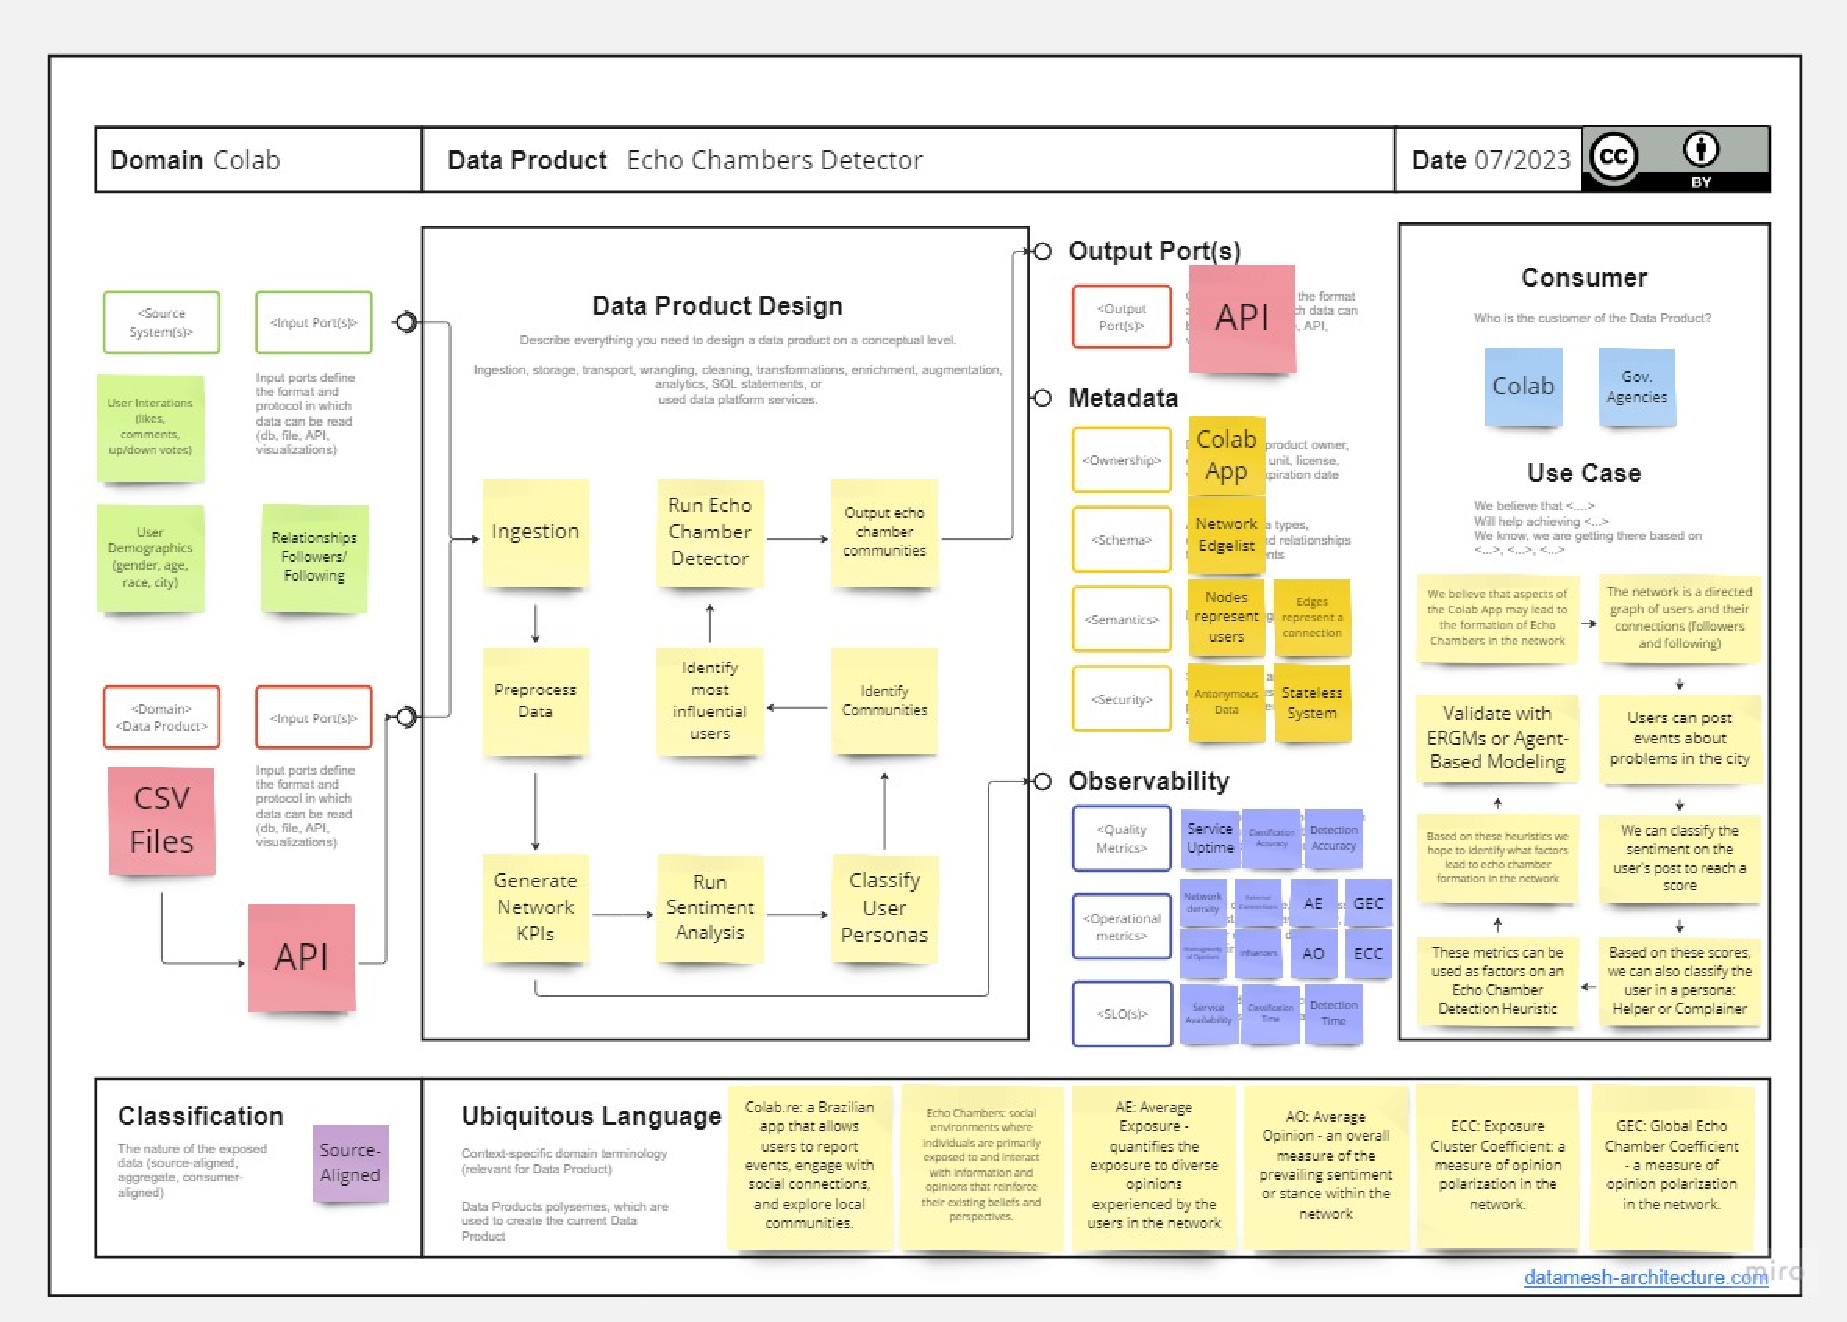
\includegraphics[scale=0.5]{tex/includes/data_canvas.pdf}
	\fautor
\end{figure}

Durante as discussões exploratórias com a equipe do Colab, elaboramos o Data Product Canvas como parte integrante da metodologia adotada para o desenvolvimento do aplicativo de detecção de câmaras de eco. O canvas proporcionou uma estrutura sólida e organizada para entendermos os requisitos do aplicativo e definirmos os diferentes elementos envolvidos em seu design e implementação.

Na seção de "Portos de Entrada", identificamos as interações dos usuários, como curtidas, comentários e votos positivos/negativos, juntamente com dados demográficos relevantes, como gênero, idade, raça e localidade. Além disso, consideramos as conexões entre usuários, representadas por seguidores e pessoas seguidas. Esses portos de entrada são fundamentais para a coleta dos dados necessários para análise e detecção de câmaras de eco na rede.

O design do produto de dados foi delineado em várias etapas, desde a ingestão dos dados até a geração de KPIs da rede, execução da análise de sentimentos, classificação das personas dos usuários, identificação de comunidades, detecção de usuários influentes, até a execução do detector de câmaras de eco e a saída das comunidades identificadas. Essa abordagem sequencial e bem definida permitirá uma análise abrangente e sistemática das câmaras de eco presentes na rede, fornecendo insights valiosos sobre sua formação e dinâmica.

Ao considerar os "Portos de Saída", optamos por utilizar uma API para disponibilizar as comunidades de câmaras de eco detectadas pelo aplicativo. Essa escolha nos permite fornecer acesso eficiente e acessível aos resultados obtidos, tanto para o próprio Colab App quanto para agências governamentais interessadas em entender e abordar a formação de câmaras de eco na rede.

A seção de "Metadados" do nosso canvas é particularmente relevante, pois aborda aspectos essenciais para a compreensão e governança adequada dos dados. Nesse contexto, especificamos que o aplicativo pertence ao Colab App e adotamos um esquema de dados baseado em uma lista de arestas da rede. A semântica do produto de dados é definida pelas entidades que representam os usuários e pelas conexões que representam as relações entre eles. Além disso, consideramos a segurança dos dados, garantindo que todas as informações coletadas sejam anônimas e que o sistema seja stateless.

A observabilidade é um aspecto crítico para garantir a qualidade e o desempenho do aplicativo. Nesse sentido, definimos métricas relevantes, como tempo de atividade do serviço, precisão da detecção, precisão da classificação, densidade da rede, conexões externas, homogeneidade de opiniões, influenciadores, opinião média, exposição média, coeficiente de agrupamento de exposição e coeficiente de câmaras de eco global. Essas métricas nos permitirão monitorar e avaliar o desempenho do aplicativo, bem como a eficácia da detecção de câmaras de eco na rede.

No contexto dos consumidores, identificamos o Colab App e agências governamentais como as partes interessadas em utilizar as comunidades de câmaras de eco detectadas. Esses consumidores poderão aproveitar os insights fornecidos pelo aplicativo para entender a formação das câmaras de eco e desenvolver estratégias eficazes para mitigar seus efeitos negativos.

Considerando o caso de uso do aplicativo, ressaltamos a crença de que certos aspectos do Colab App podem levar à formação de câmaras de eco na rede. Nesse contexto, o aplicativo foi projetado para permitir que os usuários postem eventos relacionados a problemas em suas cidades. Além disso, a análise de sentimentos é aplicada a essas postagens, fornecendo uma pontuação que permite classificar os usuários em personas. Essas métricas são fatores essenciais na heurística de detecção de câmaras de eco, que busca identificar quais fatores contribuem para a formação dessas câmaras. Por fim, planejamos validar nossos resultados utilizando modelos ERGMs (Exponential Random Graph Models) ou modelos baseados em agentes para confirmar a robustez das detecções feitas pelo aplicativo.

O uso do Data Product Canvas revelou-se essencial para estabelecer uma abordagem estruturada e colaborativa no desenvolvimento do aplicativo de detecção de câmaras de eco. Através desse framework, foi possível uma clara definição dos requisitos, elementos de design e aspectos operacionais do aplicativo, guiando todo o processo de desenvolvimento de forma sistemática.

Ao adotar o Data Product Canvas, buscamos não somente construir um aplicativo funcional, mas também obter uma compreensão aprofundada das dinâmicas de formação e impacto das câmaras de eco na rede do Colab App. Com uma definição clara dos portos de entrada, como as interações dos usuários e seus dados demográficos, e a utilização de técnicas de análise de sentimentos e classificação de personas, esperamos gerar insights valiosos para a mitigação dos efeitos negativos dessas câmaras.

Essa abordagem orientada pelo Data Product Canvas permite uma visão holística do aplicativo, contemplando desde a ingestão e pré-processamento dos dados até a identificação e classificação das comunidades de câmaras de eco. Com a identificação dos portos de saída, como uma API para disponibilizar as comunidades detectadas, buscamos assegurar a acessibilidade dos resultados tanto para os usuários do Colab App quanto para as agências governamentais interessadas.

Portanto, a aplicação do Data Product Canvas no desenvolvimento do aplicativo de detecção de câmaras de eco fortaleceu a estrutura do projeto, promovendo um processo colaborativo e possibilitando uma compreensão aprofundada das dinâmicas sociais envolvidas. Essa abordagem estruturada e integrada nos permite vislumbrar uma contribuição significativa para a identificação e mitigação das câmaras de eco no contexto do Colab App, fornecendo uma base sólida para a promoção de uma troca de informações mais diversificada e inclusiva na rede.

\section{Considerações Éticas e limitações}
Ao conduzir esta pesquisa, dedicamos especial atenção às considerações éticas e às questões de privacidade dos usuários. Todas as diretrizes éticas foram rigorosamente seguidas, e medidas foram adotadas para garantir a confidencialidade e o anonimato dos dados utilizados. Respeitamos a privacidade dos usuários do aplicativo Colab, tratando todas as informações de maneira sensível e em conformidade com as regulamentações e políticas de proteção de dados.

Obtivemos todas as autorizações necessárias para acessar e utilizar os dados relacionados aos usuários do aplicativo Colab, garantindo a legalidade e a conformidade com as diretrizes estabelecidas. Além disso, asseguramos que todas as informações sensíveis fossem tratadas com responsabilidade, adotando medidas de segurança adequadas para evitar qualquer divulgação não autorizada.

É importante ressaltar que todos os procedimentos adotados nesta pesquisa estão em conformidade com as diretrizes éticas estabelecidas pelo Comitê de Ética em Pesquisa de nossa instituição. O projeto foi submetido a uma análise minuciosa, considerando todos os aspectos éticos relacionados à coleta, análise e divulgação dos dados. A integridade e a validade dos resultados foram salvaguardadas por meio da adesão rigorosa às normas e regulamentos éticos.

Quanto às limitações do estudo, é válido destacar a natureza predominantemente quantitativa da pesquisa. Embora tenhamos empregado técnicas de análise de redes, algoritmos de agrupamento e detecção de comunidades, bem como a utilização de modelos epidemiológicos digitais, reconhecemos que uma abordagem exclusivamente quantitativa pode limitar a compreensão completa do fenômeno em estudo.

Para complementar a análise objetiva das interações dos usuários e a disseminação de informações nas câmaras de eco, é importante considerar abordagens qualitativas. Entrevistas e análise de conteúdo podem fornecer insights valiosos sobre as percepções, atitudes e motivações dos usuários envolvidos nas câmaras de eco. A combinação dessas abordagens quantitativas e qualitativas permitiria uma compreensão mais abrangente e rica do fenômeno.

É fundamental reconhecer e abordar as limitações inerentes a qualquer pesquisa, garantindo que os resultados sejam interpretados com cautela e considerando possíveis viéses ou lacunas no estudo. Ao fazê-lo, podemos avançar no conhecimento sobre as câmaras de eco no contexto do Colab App, contribuindo para uma compreensão mais completa desse fenômeno complexo e fornecendo subsídios para ações mitigadoras efetivas.

\section{Disponibilidade do Código-Fonte}
O código-fonte desenvolvido neste projeto está disponível em um repositório público no GitHub. Ele contém as implementações dos algoritmos de construção da rede social, algoritmos de agrupamento, modelos de epidemiologia digital e o desenvolvimento do painel em tempo real. O repositório pode ser acessado no seguinte endereço:\url{https://github.com/guinetik/colab-network-ec}.

\chapter{Uma Visão Geral do Colab}
\label{chapter:04_colab}
A participação cidadã e a colaboração por meio de empresas de tecnologia especializadas em negócios de governança pública, conhecidas como Gov-Techs,  têm se tornado cada vez mais relevantes na sociedade contemporânea. Com os avanços tecnológicos e a disseminação das redes sociais, surgiram novas formas de engajamento e interação entre cidadãos e governos. Nesse contexto, o aplicativo Colab se destaca como uma plataforma inovadora que combina elementos de redes sociais com a participação cidadã em questões relacionadas à gestão pública.

Neste capítulo, abordaremos o Colab a partir de uma perspectiva que envolve as redes sociais, e-Gov (governo eletrônico) e Gov-Techs, bem como a vigilância participativa. Analisaremos suas funcionalidades, impactos sociais, desafios e limitações, explorando o papel desempenhado pelo Colab nesse contexto dinâmico de engajamento cidadão e colaboração com as instâncias governamentais.

\section*{História e Desenvolvimento}
O Colab foi lançado em 2013 como uma iniciativa pioneira no campo da participação cidadã digital. A plataforma foi desenvolvida pelos sócios Paulo Pandolfi e Gustavo Maia, que, inspirados por suas experiências em marketing político, perceberam a necessidade de uma ferramenta que permitisse uma maior interação entre cidadãos e governos \cite{2023_Colab_PAGE}.

O objetivo do Colab é permitir que os usuários compartilhem ideias, façam sugestões, denunciem problemas e participem ativamente na construção de políticas públicas. Funcionando como uma rede social, os cidadãos podem postar fotos de problemas da cidade e solicitar uma solução. As prefeituras, por sua vez, acessam essas reclamações e têm uma solução de tecnologia em nuvem para dar andamento às solicitações \cite{2023_Colab_PAGE}.

Desde o seu lançamento, o Colab tem conquistado espaço em diversas cidades, tornando-se uma ferramenta de referência no campo da democracia digital. A plataforma foi eleita “o melhor app urbano do mundo” pela NewCities Foundation e hoje conta com 200 mil cadastros e contratos com diversas cidades, incluindo Recife, Ipojuca, Niterói, Mesquita, Maceió, Aracaju, Cruz Alta, Santo André e Juiz de Fora \cite{2023_Colab_PAGE}.

Além disso, desde 2016, o Colab também oferece uma ferramenta para que as prefeituras abram consultas sobre questões da cidade, auxiliando na tomada de decisões e na coleta de dados. Essa ferramenta tem vários formatos e gera muitos dados que ajudam a fazer uma gestão melhor com a participação do cidadão \cite{2023_Colab_PAGE}.

A história do Colab é marcada por desafios e inovações. Quando foi lançado, o aplicativo não tinha nenhuma prefeitura cadastrada. As necessidades dos cidadãos eram coletadas pela empresa e enviadas para a administração pública pelos canais de atendimento tradicionais, como site e email. No entanto, mesmo sem prefeituras cadastradas, o sistema foi reconhecido internacionalmente pela NewCities Foundation como "o melhor app urbano do mundo" \cite{2023_Colab_PAGE}.

A primeira prefeitura a adotar oficialmente o Colab foi Curitiba, seguida por outras 50 no mesmo ano. Esse crescimento rápido trouxe desafios, pois a empresa precisava atender melhor e evoluir, mas ainda não tinha receita. No entanto, um contrato com a organização social Comunitas, no começo de 2015, para atender as cidades de Santos e Campinas, em São Paulo, e Pelotas, no Rio Grande do Sul, injetou dinheiro na empresa e deu ânimo aos empreendedores \cite{2023_Colab_PAGE}.

Desde a sua fundação, o Colab tem buscado desenvolver soluções tecnológicas que possam contribuir para a construção de uma gestão pública mais eficiente, transparente e participativa. Atualmente, a plataforma está presente em mais de 130 cidades, em 2 países, e conta com cerca de 900 mil usuários cadastrados \cite{2023_Colab_PAGE}.

Hoje, a plataforma tem 200 mil cadastros e contratos com diversas cidades, incluindo Recife, Ipojuca, Niterói, Mesquita, Maceió, Aracaju, Cruz Alta, Santo André e Juiz de Fora. O valor dos contratos varia de 38 mil a 500 mil reais por ano, calculado com base na população da cidade e na quantidade de módulos contratados.

\section*{Funcionalidades}

\begin{figure}[!htb]
	\caption{Tela inicial do app Colab}
	\label{fig:colab_app}
	\centering
	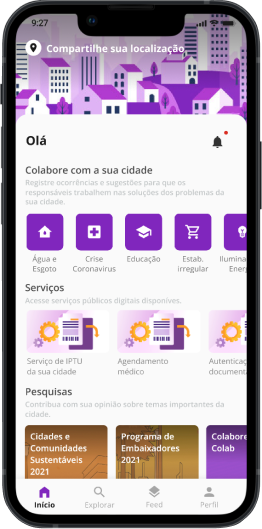
\includegraphics[scale=0.5]{colab_app.png}
\end{figure}

O Colab é uma plataforma digital que promove a vigilância participativa, a democracia digital e o governo eletrônico (e-Gov) por meio de uma série de funcionalidades interativas. A plataforma se destaca por permitir que os cidadãos desempenhem um papel ativo na gestão pública, contribuindo com ideias, sugestões e denúncias, e participando de consultas públicas.

A funcionalidade de publicação de ideias e sugestões permite que os usuários compartilhem suas ideias sobre questões de interesse público, abrangendo uma variedade de temas, desde melhorias na infraestrutura urbana até propostas de políticas sociais. Essa funcionalidade promove a democracia digital, permitindo que os cidadãos participem ativamente na formulação de políticas públicas.

A funcionalidade de denúncia de problemas permite que os usuários denunciem problemas como buracos nas vias, iluminação pública deficiente, entre outros. Essas denúncias são georreferenciadas, facilitando a identificação e resolução dos problemas pelas autoridades competentes. Isso contribui para a vigilância participativa, pois permite que os cidadãos monitorem a qualidade dos serviços públicos e infraestruturas em suas comunidades.

O Colab também possui uma forte componente social. Os usuários podem seguir outros usuários, serem seguidos, curtir e comentar as publicações. Isso promove a formação de uma rede social dentro do Colab, ampliando as possibilidades de engajamento e diálogo entre os participantes.

Os usuários também podem acompanhar o andamento das demandas e propostas que foram apresentadas. Isso permite que eles estejam cientes das ações tomadas pelo governo em resposta às suas contribuições, promovendo a transparência e a responsabilidade no governo eletrônico.

Além disso, o Colab introduziu recentemente novas funcionalidades, como micro consultas, reportar comentários e priorização de comentários. As micro consultas permitem que os usuários respondam perguntas rápidas do tipo sim/não diretamente na notificação push, trazendo mais dinamismo e velocidade para a gestão do relacionamento entre o cidadão e a cidade. A funcionalidade de reportar comentários permite que os usuários do Colab reportem comentários uns dos outros, mantendo a qualidade e a relevância das discussões na plataforma. A priorização de comentários, também conhecida como up/down vote, permite que os usuários indiquem o quão relevante um comentário é por meio de votos, destacando as contribuições mais valiosas.

A funcionalidade de consultas públicas é uma parte essencial do Colab, permitindo que os governos interajam diretamente com os cidadãos e obtenham feedback sobre várias questões. As consultas podem ser personalizadas para se adaptarem à realidade de cada território, e os gestores públicos podem criar seus próprios processos. Além disso, é possível configurar as consultas para permitir respostas anônimas. Essa funcionalidade promove a democracia digital e o governo eletrônico, permitindo que os cidadãos participem diretamente na tomada de decisões do governo.

A gamificação é um aspecto central do Colab, usada para aumentar o engajamento dos cidadãos e incentivá-los a participar ativamente na melhoria de suas cidades. A gamificação envolve o uso de elementos de design de jogos em contextos não-jogáveis para motivar a participação, envolvimento e lealdade.

No Colab, a gamificação é implementada através da "Jornada do Cidadão", uma trilha com desafios que orientam o cidadão sobre como ele pode colaborar e participar mais para tornar sua cidade melhor. Ao completar esses desafios, os cidadãos recebem recompensas e conquistas, que podem ser compartilhadas com outros usuários. Isso não apenas incentiva a participação contínua, mas também ajuda a disseminar uma cultura de participação dentro da cidade.

A gamificação no Colab não se limita apenas a incentivar a participação dos cidadãos. Ela também pode ser usada para conscientizar sobre determinadas causas ou estimular a participação em eventos. Por exemplo, se um hemocentro da cidade precisa de mais doações de sangue, a gestão pública pode criar um desafio no Colab para incentivar os cidadãos a doar sangue. Ao fazer isso, os cidadãos podem ganhar conquistas como "doador" ou "zelador do patrimônio público", reforçando a importância de suas contribuições para a cidade.

Em resumo, o Colab é uma plataforma que combina elementos de vigilância participativa, democracia digital e governo eletrônico para promover a participação cidadã na gestão pública. Através de suas diversas funcionalidades, o Colab busca fortalecer a participação cidadã, criar um ambiente propício para o diálogo entre cidadãos e governos, e promover a transparência e a responsabilidade no governo.

\section*{Gov Techs}
As gov techs são empresas que fornecem soluções tecnológicas para o setor público. Elas desempenham um papel crucial na modernização dos serviços governamentais, melhorando a eficiência, a transparência e a participação cidadã. Os serviços prestados ao governo por empresas de gov tech podem variar amplamente, dependendo das necessidades específicas do governo. Alguns exemplos incluem:

\begin{itemize}
	\item Digitalização de processos burocráticos: Isso pode incluir a criação de sistemas de gerenciamento de documentos, plataformas de pagamento online e sistemas de agendamento de compromissos.
	\item Plataformas de participação cidadã: Estas são plataformas que permitem aos cidadãos participar diretamente na tomada de decisões do governo. Isso pode incluir a votação em questões políticas, a apresentação de propostas de políticas e a participação em discussões públicas.
	\item Soluções de análise de dados: As empresas de gov-tech podem fornecer soluções que ajudam o governo a coletar, analisar e interpretar grandes quantidades de dados. Isso pode ajudar o governo a tomar decisões mais informadas e eficazes.
\end{itemize}

O Colab é um exemplo de uma solução de gov tech que se destaca na indústria pelo seu aspecto social. Como uma plataforma de participação cidadã, o Colab permite que os cidadãos se envolvam diretamente na tomada de decisões do governo, promovendo a transparência e a responsabilidade. Isso representa uma mudança significativa na forma como o governo interage com os cidadãos, permitindo uma maior inclusão e participação na tomada de decisões.

No entanto, a adoção de soluções de gov tech como o Colab não está isenta de desafios. De acordo com um estudo de \citeonline{2021_Liang}, fatores como a competência do provedor, a prontidão organizacional, a pressão externa e a confiança na tecnologia desempenham um papel significativo na adoção de tecnologias de nuvem móvel no governo. Esses fatores podem ser igualmente aplicáveis ao Colab e outras soluções de gov tech, e precisam ser considerados cuidadosamente ao implementar essas tecnologias.

Além disso, a tecnologia blockchain está emergindo como uma nova ferramenta potencial para o setor público. \citeonline{2021_Diakiv} identifica dez direções potenciais para o uso de tecnologias blockchain no setor público, incluindo autenticação, rastreabilidade e singularidade. Embora o Colab não utilize a tecnologia blockchain, a crescente importância dessa tecnologia no setor público sugere que pode ser uma área para futura exploração ou integração.

Finalmente, a ética na tecnologia é uma consideração importante na adoção de soluções de gov tech. \citeonline{2022_Grellette} sugere a realização de auditorias de confiança como uma maneira de melhorar a prática da ética na tecnologia. Isso poderia ser relevante para o Colab e outras soluções de gov tech, à medida que buscam ganhar e manter a confiança do público.

\section*{Interfaces para problemas urbanos}
Devido a adoção em massa de aplicativos e a alta disponibilidade da internet, softwares sociais e de vigilância participativa tem se tornado interfaces para problemas urbanos. Essas interfaces têm desempenhado um papel crucial na resolução de questões relacionadas às cidades. Vários estudos de caso têm evidenciado a eficácia dessa ferramenta em abordar desafios urbanos e promover a participação cidadã.

\citeonline{2021_Barros} avaliaram o Colab juntamente com outras duas iniciativas de democracia digital, Mudamos e Panela de Pressão. A avaliação considerou diferentes aspectos, como recursos tecnológicos, modos de participação online, atores envolvidos, objetivos políticos das iniciativas e captação de recursos. Os resultados destacaram a importância da estrutura organizacional na compreensão do desenvolvimento bem-sucedido de iniciativas de democracia digital.

\citeonline{2015_Silva} analisaram o Colab como uma ferramenta de colaboração e mobilidade urbana. Esse estudo ressaltou a relevância do Colab como uma plataforma que permite aos cidadãos participarem ativamente da melhoria de suas cidades, fornecendo um canal direto de feedback às autoridades municipais sobre problemas urbanos.

O estudo de \citeonline{2018_CARVALHO_DISSERTATION} explora o uso do aplicativo móvel Colab.re para promover a participação social na gestão da cidade de Paragominas, no estado do Pará, Brasil. Apesar de Paragominas ser uma cidade relativamente isolada, o estudo demonstrou que a implementação do Colab.re resultou em um canal eficaz de comunicação entre a prefeitura e os cidadãos, alcançando o maior percentual de usuários do aplicativo em todo o estado do Pará. As conclusões de Carvalho indicam que a Computação Urbana e o uso de dispositivos móveis podem fortalecer as relações entre os usuários e ajudar a entender melhor como os problemas pontuais afetam a cidade como um todo. O estudo destaca o potencial da Computação Urbana e de aplicativos móveis para melhorar a gestão das cidades, promovendo a participação social e melhorando a comunicação entre os cidadãos e as autoridades municipais, mesmo em áreas isoladas como Paragominas.

Esses estudos de caso fornecem evidências concretas de como o Colab tem sido uma interface valiosa na resolução de problemas urbanos. Sua capacidade de promover a participação cidadã, coletar feedback dos cidadãos e melhorar a prestação de serviços públicos o torna uma ferramenta relevante para impulsionar mudanças positivas nas cidades. Através do Colab e de outras interfaces similares, é possível fortalecer a colaboração entre os cidadãos, autoridades municipais e outros atores envolvidos na busca por soluções inovadoras e sustentáveis para os desafios urbanos.

\section*{Engajamento Cidadão e Plataformas Digitais na Era da COVID-19}
A pandemia de COVID-19 apresentou desafios sem precedentes para a participação cidadã e o engajamento social. Em resposta a esses desafios, plataformas digitais emergiram como ferramentas vitais para facilitar a participação cidadã na gestão pública, mesmo em meio ao distanciamento social.

\subsection*{Vigilância Participativa}
A vigilância participativa é uma abordagem inovadora que envolve o engajamento ativo da comunidade no processo de coleta, monitoramento e compartilhamento de informações relevantes para identificar e responder a problemas sociais, ambientais e de saúde. 

\begin{citacao}
	"uma forma de inteligência coletiva em que as pessoas se reúnem para monitorar, analisar e agir coletivamente em relação a um problema ou questão compartilhada" \cite[p. 1]{2011_Bryer}.
\end{citacao}

Com os avanços tecnológicos e a disseminação de dispositivos móveis e plataformas digitais, a aplicação de aplicativos móveis para a vigilância participativa tem ganhado destaque. Nesta seção, exploramos o conceito de vigilância participativa, apresentando sua definição e abordando sua relevância no contexto atual.

A vigilância participativa tem sido reconhecida como uma abordagem promissora para a coleta de informações em tempo real, permitindo que a comunidade desempenhe um papel ativo na detecção e monitoramento de problemas sociais, ambientais e de saúde. Tradicionalmente, a vigilância tem sido realizada por meio de sistemas centralizados e conduzida por especialistas em saúde ou autoridades governamentais. No entanto, com a proliferação de dispositivos móveis, o acesso à internet e o surgimento de plataformas colaborativas, os aplicativos móveis têm sido adotados como ferramentas eficazes para engajar os cidadãos na vigilância participativa.

O conceito de vigilância participativa foi formalmente reconhecido pelas Regulamentações Sanitárias Internacionais (RSIs) revisadas em 2005, as quais ampliaram o escopo da vigilância além dos mecanismos tradicionais. Esse reconhecimento proporcionou uma oportunidade para a integração de canais não oficiais e melhorias tecnológicas para agilizar a detecção, o monitoramento e a resposta a problemas de saúde. A vigilância participativa utiliza métodos de crowdsourcing para coletar informações da sociedade e devolver o conhecimento coletivo de volta à comunidade.\cite[1]{2017_Smolinski}

Um estudo de caso relevante que exemplifica a aplicação da vigilância participativa é a iniciativa "Saúde na Copa" durante a Copa do Mundo FIFA de 2014, realizada no Brasil. O projeto utilizou um aplicativo de vigilância participativa chamado Healthy Cup, permitindo que usuários de todo o mundo relatassem suas condições de saúde em tempo real. Ao focar em três síndromes específicas e seis doenças relevantes para aglomerações de pessoas, o aplicativo facilitou a detecção precoce de surtos de doenças agudas ao identificar agregados de sintomas indicativos de doenças infecciosas \cite{2017_LealNeto}.

Além da saúde, a vigilância participativa também tem sido aplicada em outras áreas, proporcionando benefícios semelhantes e promovendo a participação ativa da comunidade. Essa abordagem colaborativa tem se mostrado útil na vigilância de diversos aspectos do ambiente e da sociedade, permitindo que os cidadãos desempenhem um papel ativo na coleta e compartilhamento de informações relevantes.

Um exemplo notável é o uso da vigilância participativa na monitorização da qualidade do ar por meio do aplicativo AirVisual. Com a contribuição dos usuários, juntamente com dados oficiais de estações de monitoramento, é possível mapear e identificar áreas com problemas de poluição atmosférica. Os cidadãos podem relatar os níveis de poluição do ar em suas áreas, fornecendo informações valiosas para a vigilância participativa desse aspecto crucial do ambiente. Essa abordagem empodera os indivíduos a agirem como agentes ativos na identificação de áreas com poluição do ar significativa, contribuindo para a tomada de decisões informadas e para a melhoria da qualidade do ar nas comunidades.

\begin{figure}[!htb]
    \caption{Aplicativo NoiseTube exibindo o nível de ruído em uma localidade}
    \label{fig:app_noisetube}
    \centering
    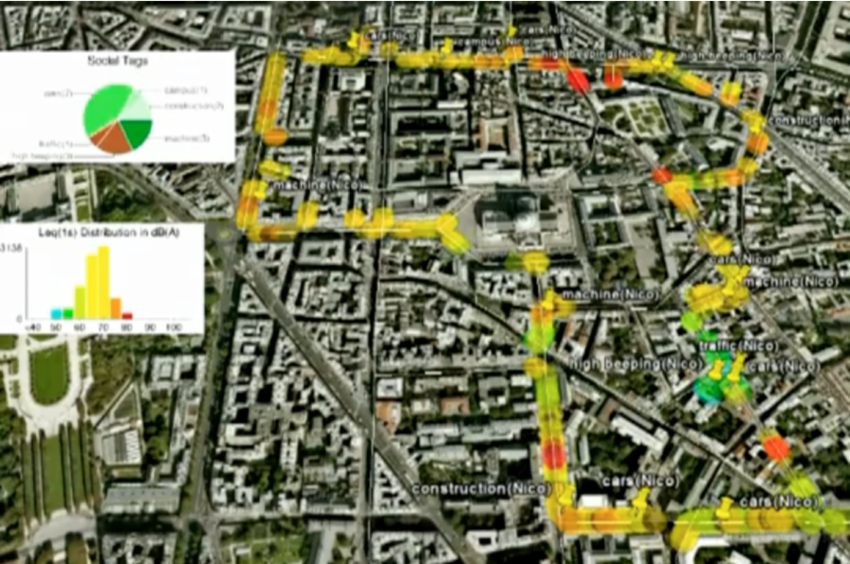
\includegraphics[scale=0.8]{app_noisetube.png}
    \fdireta{2010_Arnand}
\end{figure}

Outra área em que a vigilância participativa tem desempenhado um papel importante é a monitorização do ruído ambiental. O aplicativo NoiseTube permite que os usuários realizem medições de ruído e compartilhem esses dados, criando um mapa colaborativo do ruído em diferentes localidades. Essa vigilância participativa do ruído ambiental permite a identificação de áreas com altos níveis de ruído, auxiliando na tomada de medidas para mitigar os efeitos adversos na saúde e no bem-estar da comunidade. Ao participar ativamente da vigilância do ruído, os cidadãos contribuem para a criação de ambientes mais saudáveis e para a implementação de políticas públicas adequadas \cite{2010_Arnand}.

Esses exemplos ilustram como a vigilância participativa pode ser aplicada em diferentes áreas, além da saúde. Ao envolver os cidadãos na coleta e compartilhamento de informações relevantes, a vigilância participativa se torna uma ferramenta poderosa para a identificação e resposta a problemas ambientais e sociais. Essa abordagem colaborativa, combinada com o uso de tecnologias móveis e plataformas digitais, fortalece a relação entre a comunidade e as autoridades responsáveis, promovendo uma governança mais inclusiva e eficaz.

\subsection*{Iniciativa Brasil Sem Corona}

A Iniciativa Brasil Sem Corona, uma colaboração entre o Colab e a startup Epitrack, exemplifica o uso eficaz da tecnologia para facilitar a participação cidadã durante uma crise de saúde pública. Através desta iniciativa, os dados sobre a pandemia de COVID-19 foram coletados diretamente dos cidadãos, que relataram seus sintomas e receberam informações sobre como se proteger do vírus. Esses dados foram então utilizados para gerar mapas de calor que auxiliaram as autoridades de saúde a identificar e responder a surtos de COVID-19.

Na cidade de Caruaru/PE, a iniciativa teve resultados significativos. O projeto contou com 861 usuários ativos, apresentando uma média de 1,2 relatórios por usuário por semana. A plataforma Brasil Sem Corona começou em 20 de março e, desde então, tem sido oficialmente utilizada pela autoridade de saúde de Caruaru para melhorar a qualidade das informações do sistema de vigilância tradicional. Em relação aos casos de síndrome respiratória do sistema de vigilância tradicional, 1.588 indivíduos foram positivos para este resultado clínico. A análise de varredura espacial detectou 18 aglomerados e 6 deles apresentaram significância estatística (valor p < 0,1). Os aglomerados 3 e 4 apresentaram uma área de sobreposição que foi escolhida pela autoridade local para implantar a sorologia de Covid-19, onde 50 indivíduos foram testados. Desses, 32\% (n=16) apresentaram resultados reagentes para anticorpos relacionados à Covid-19 \cite[1]{2020_LealNeto}. Essa pesquisa demonstra como a vigilância participativa pode ser uma ferramenta eficaz para melhorar a qualidade das informações do sistema de vigilância tradicional, permitindo uma detecção precoce de surtos de COVID-19 e uma resposta mais eficaz, principalmente quando aliado a uma aplicação de alta disponibilidade e adoção pela população.

\section{Reflexões sobre o Colab}

As soluções de empresas Gov Tech têm emergido como catalisadores poderosos na transformação das relações entre cidadãos e órgãos governamentais. Estas plataformas, como o Colab, não apenas facilitam a comunicação, mas também redefinem a dinâmica da participação cidadã, tornando-a mais direta, transparente e, sobretudo, democrática. No entanto, a mesma interconexão que possibilita essa participação ampliada também pode criar ambientes isolados, as chamadas câmaras de eco, onde os usuários são frequentemente expostos apenas a opiniões que reforçam suas crenças preexistentes.

O Colab, ao promover a participação ativa e informada dos cidadãos, tem o potencial de contrabalançar os efeitos negativos das câmaras de eco. Ao incentivar o diálogo aberto e a colaboração entre cidadãos de diferentes backgrounds e perspectivas, a plataforma pode ajudar a criar uma sociedade mais informada e resiliente. Através da análise dos perfis dos usuários e das postagens, foi possível identificar tendências, prioridades e problemas recorrentes, fornecendo subsídios importantes para a formulação de políticas públicas mais eficazes e direcionadas.

A diversidade de gênero e a representatividade na participação cívica são fundamentais para garantir uma governança inclusiva e representativa. A combinação de abordagens digitais e tradicionais pode gerar resultados mais abrangentes e inclusivos, evitando a exclusão digital e garantindo a participação de todos os segmentos da sociedade.

No entanto, é fundamental que as plataformas sejam projetadas levando em consideração a usabilidade, a acessibilidade e a segurança dos dados dos usuários. Políticas claras de privacidade e proteção de dados devem ser implementadas, garantindo a confidencialidade das informações compartilhadas e a confiança dos usuários na plataforma.

Em um mundo cada vez mais digital, onde as câmaras de eco podem distorcer a percepção da realidade e influenciar decisões, plataformas como o Colab surgem como ferramentas essenciais para garantir que a voz do cidadão seja ouvida, respeitada e incorporada nas políticas públicas. Ao explorar o potencial das plataformas de engajamento cívico, os governos podem fortalecer a democracia, criar comunidades mais participativas e resilientes e, sobretudo, garantir que as decisões tomadas reflitam verdadeiramente as necessidades e desejos da população.

\section{Fonte de Dados}
Nesta pesquisa, utilizamos como fonte de dados o conjunto de informações coletadas e disponibilizadas pela equipe de R\&D do Colab. Esses dados consistem em listas de arestas, que representam as conexões entre os usuários,suas interações como likes e comentários, e suas postagens realizadas entre os anos de 2016 e 2022. Limitamos alguns aspectos da pesquisa às cidades de Caruaru, Rio de Janeiro, Recife, Niterói, Mesquita e Santo André, a fim de obter uma amostra representativa dessas regiões.

A coleta dos dados foi possível através de parcerias estabelecidas com a equipe do Colab, que nos concedeu acesso ao conjunto de informações. Esses dados são de grande relevância para o desenvolvimento da pesquisa, pois nos permitem examinar as interações sociais e os padrões de engajamento dos usuários dentro da plataforma.

\subsection*{Modelo de dados}
\label{sec:modelo_de_dados}

Os dados dos foram disponibilizados em formato CSV, contendo informações sobre os usuários e os eventos reportados. A seguir, é apresentado um resumo mo modelo de dados utilizados:

\begin{itemize}
	\item User (\autoref{tab:user_model}): Dados dos usuários
	\item Connection (\autoref{tab:connections_model}): Conexão entre os usuários, com lista de seguidores/seguindo.
	\item Events (\autoref{tab:event_model}): Eventos reportados pelos usuários.
	\item Likes (\autoref{tab:interactions_model}): Apoios/curtidas na rede social.
	\item Comments (\autoref{tab:interactions_model}): Comentários em publicações de outros usuários.
	\item UpDown Vote (\autoref{tab:updown_model}): Endosso ou rejeição a comentários de outros usuários.
\end{itemize}

\begin{table}[ht]
	\centering
	\caption{Tabela Users: Representa os usuários do app}
	\label{tab:user_model}
	\begin{tabularx}{\textwidth}{|l|X|}
		\hline
		\textbf{Campo}     & \textbf{Descrição}                              \\
		\hline
		colab\_user\_id    & Identificador único do usuário no app Colab 	 \\
		gender             & Gênero do usuário                               \\
		race               & Raça do usuário                               	 \\
		education          & Escolaridade do usuário                         \\
		birth\_date        & Data de nascimento do usuário                   \\
		city\_id           & Identificador único da cidade do usuário        \\
		city\_name         & Nome da cidade do usuário                       \\
		state\_id          & Identificador único do estado do usuário        \\
		state\_name        & Nome do estado do usuário                       \\
		created\_at        & Data de criação do registro do usuário          \\
		last\_sign\_in\_at & Data da última vez que o usuário fez login      \\
		device             & Dispositivo utilizado pelo usuário              \\
		\hline
	\end{tabularx}
\end{table}

\begin{table}[ht]
	\centering
	\caption{Tabela Connetion: Representa a conexão entre os usuários}
	\label{tab:connections_model}
	\begin{tabularx}{\textwidth}{|l|X|}
		\hline
		\textbf{Campo}    & \textbf{Descrição}                                   \\
		\hline
		source         	  & Identificador único do evento                        \\
		target            & Identificador único do usuário relacionado ao evento \\
		created\_at       & Data de criação, representando um follow             \\
		deleted\_at       & Data de deleção, representando um unfollow			 \\
		\hline
	\end{tabularx}
\end{table}

\begin{table}[ht]
	\centering
	\caption{Tabela Events: Representa os eventos reportados pelos usuários}
	\label{tab:event_model}
	\begin{tabularx}{\textwidth}{|l|X|}
		\hline
		\textbf{Campo}    & \textbf{Descrição}                                   \\
		\hline
		event\_id         & Identificador único do evento                        \\
		user\_id          & Identificador único do usuário relacionado ao evento \\
		description       & Descrição do evento                                  \\
		status            & Status do evento                                     \\
		created\_at       & Data de criação do evento                            \\
		event\_type\_id   & Identificador único do tipo de evento                \\
		event\_type\_name & Nome do tipo de evento                               \\
		\hline
	\end{tabularx}
\end{table}

\begin{table}[ht]
	\centering
	\caption{Tabela Interactions: Representa as interações entre os usuários}
	\label{tab:interactions_model}
	\begin{tabularx}{\textwidth}{|l|X|}
		\hline
		\textbf{Campo}    & \textbf{Descrição}                                   		 		\\
		\hline
		user\_from        & O colab\_user\_id do usuário criador da curtida/apoio          		\\
		user\_to          & O colab\_user\_id do usuário recebidor da curtida/apoio  		 	\\
		created\_at       & Data de criação da interação        				 				\\
		\hline
	\end{tabularx}
\end{table}

\begin{table}[ht]
	\centering
	\caption{Tabela Up-Down Vote: Representa os endossos e rejeições de comentários}
	\label{tab:updown_model}
	\begin{tabularx}{\textwidth}{|l|X|}
		\hline
		\textbf{Campo}    & \textbf{Descrição}                                   		 		\\
		\hline
		user\_from        & O colab\_user\_id do usuário criador da curtida/apoio          		\\
		user\_to          & O colab\_user\_id do usuário recebidor da curtida/apoio  		 	\\
		rating            & Representa se o endosso foi Positivo/Up (1) ou Negativo/Down (0)  	\\
		created\_at       & Data de criação da interação           				 				\\
		\hline
	\end{tabularx}
\end{table}

A partir desses dados, criamos uma representação abrangente do ambiente social e das interações dos usuários dentro do aplicativo Colab. Utilizando o conjunto de informações coletadas, realizamos uma análise exploratória para compreender os padrões e comportamentos dos usuários. Apresentamos uma análise exploratória desses dados no \autoref{chapter:04_colab}.

\section{Análise exploratória dos dados}
\label{sec:colab_data_analysis}

Com base nos dados disponibilizados pelo Colab para esse estudo, analisamos um total de 328.876 eventos criados entre 04/01/2013 e 05/12/2022.

\subsection*{Distribuição demográfica}

O quadro \autoref{quadro:usersbygender} apresenta a distribuição demográfica dos usuários por gênero. A maioria dos usuários se declararam do gênero másculino.

\begin{quadro}[htb]
	\caption{Usuários por gênero}
	\label{quadro:usersbygender}
	\centering
	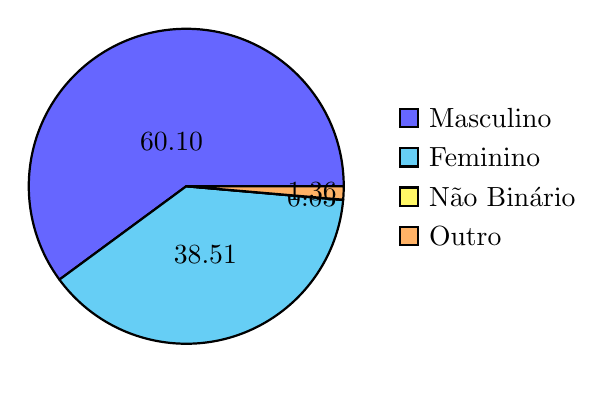
\begin{tikzpicture}
		\pie[
			sum=auto,
			text=legend,
			radius=2
		]{
			60.10/Masculino,
			38.51/Feminino,
			0.03/Não Binário,
			1.36/Outro/Desconhecido
		}
	\end{tikzpicture}
	\begin{tabular}{|l|r|}
		\hline
		\textbf{Gênero} & \textbf{Quantidade} \\
		\hline
		Masculino       & 30494               \\
		Feminino        & 19555               \\
		Não Binário     & 16                  \\
		Desconhecido    & 335                 \\
		Outro           & 274                 \\
		Não Informado   & 92                  \\
		\hline
	\end{tabular}
\end{quadro}

\subsection*{Tipos de Eventos}

\begin{table}[h]
	\centering
	\caption{Tipos de eventos com mais ocorrências}
	\label{tab:tiposevento}
	\begin{tabularx}{\textwidth}{|X|l|l|}
		\hline
		\textbf{Tipo de Evento}                  & \textbf{Total de Ocorrências} \\
		\hline
		Entulho na calçada/via pública           & 61.785                        \\
		Buraco nas vias                          & 41.200                        \\
		Lâmpada apagada à noite                  & 32.907                        \\
		Ponto de infração de trânsito recorrente & 15.873                        \\
		Calçada irregular                        & 14.837                        \\
		Mato alto                                & 13.459                        \\
		Poda de árvore                           & 12.810                        \\
		Descarte irregular de lixo               & 12.685                        \\
		Bueiro entupido                          & 8.825                         \\
		Vazamento de água                        & 7.433                         \\
		Bueiro sem tampa                         & 5.844                         \\
		Ocupação irregular de área pública       & 5.714                         \\
		Fiação irregular                         & 5.643                         \\
		Veículo abandonado                       & 5.335                         \\
		Equipamento público danificado           & 4.694                         \\
		Esgoto a céu aberto                      & 4.656                         \\
		Retirada de árvore                       & 4.437                         \\
		Ponto recorrente de poluição sonora      & 4.189                         \\
		Bloqueio na via                          & 4.066                         \\
		Iluminação pública irregular             & 3.702                         \\
		\hline
	\end{tabularx}
\end{table}

A tabela \autoref{tab:tiposevento} apresenta os 20 tipos de evento mais reportados pelos usuários. A análise dos dados fornecidos pelos usuários do Colab proporcionou insights valiosos sobre as preocupações e demandas da comunidade. Os eventos mais frequentemente relatados estão intrinsecamente ligados a problemas e irregularidades na infraestrutura urbana, como entulho na calçada/via pública, buraco nas vias, lâmpada apagada à noite, ponto de infração de trânsito recorrente e calçada irregular. Essas ocorrências destacam a importância de investimentos contínuos na manutenção e melhoria da infraestrutura da cidade. Além disso, questões ambientais emergem como uma área de preocupação significativa, com denúncias frequentes de descarte irregular de lixo, desmatamento ilegal, esgoto a céu aberto e mato alto. Essas postagens indicam uma conscientização dos usuários em relação à preservação ambiental e ressaltam a necessidade de ações efetivas para aprimorar a gestão dos recursos naturais. O transporte público também é alvo de atenção, com reclamações recorrentes sobre problemas em ônibus, atrasos e superlotação. Esses aspectos exigem uma análise aprofundada das questões relacionadas à mobilidade urbana e podem impulsionar esforços para melhorar a qualidade e eficiência do transporte coletivo. Eventos relacionados à segurança e vigilância, como pontos de exploração sexual de menores e maus-tratos a animais, refletem a preocupação dos usuários com a proteção e bem-estar da comunidade. A ocorrência de eventos envolvendo estabelecimentos comerciais, como falta de alvará e condições sanitárias irregulares, destaca a importância de ações rigorosas de fiscalização e de garantir a conformidade legal por parte dos estabelecimentos. Esses insights fornecem uma visão abrangente das preocupações dos usuários do Colab e podem orientar as prefeituras da cidade na implementação de políticas públicas que visem atender às demandas da comunidade e aprimorar a qualidade de vida em geral.

Os usuários estão engajados e ativos na identificação e denúncia de problemas na infraestrutura urbana, meio ambiente, transporte público e questões sociais. Isso indica uma participação cidadã ativa e um desejo de melhorar as condições de suas comunidades. Os clientes podem aproveitar essas informações para acompanhar as preocupações e demandas da comunidade, tomar medidas corretivas mais efetivas e aprimorar a qualidade dos serviços e infraestrutura oferecidos.

Os dados fornecem uma visão clara das principais questões enfrentadas pela comunidade, permitindo que as prefeituras priorizem recursos e esforços em áreas críticas, como manutenção da infraestrutura, gestão ambiental, transporte público e segurança. As prefeituras podem usar esses insights para desenvolver políticas públicas mais eficazes, implementar medidas preventivas e corretivas, bem como estabelecer canais de comunicação e interação mais robustos com os cidadãos, fortalecendo a confiança e a participação da comunidade nas decisões governamentais.

\subsection*{Frequência de postagens e engajamento}
\label{sec:engajamento}

\begin{quadro}[htb]
	\caption{Histograma demonstrando a distribuição de novos eventos por ano}
	\label{quadro:colab_events_overtime}
	\centering
	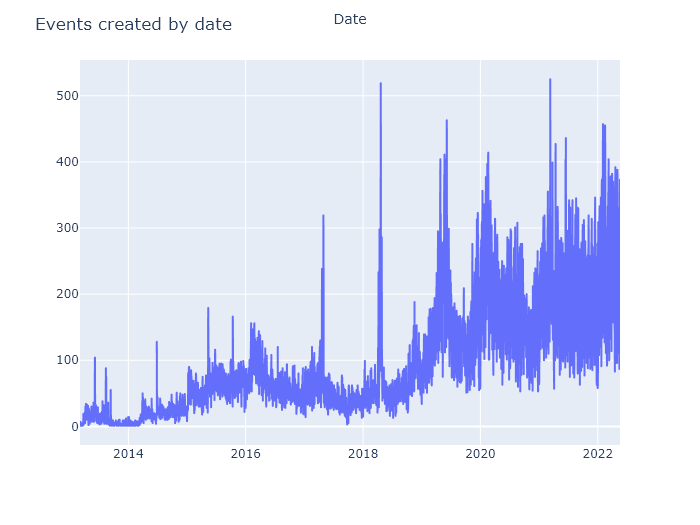
\includegraphics[scale=0.4]{colab_events_overtime.png}
\end{quadro}

O \autoref{quadro:colab_events_overtime} demonstra a criação de eventos ao longo dos anos. Na imagem pode-se identificar dois picos de mais de 500 postagens por mês: Abril de 2018 e Março de 2022. Além desses picos, é possível observar uma tendência geral de crescimento no número de postagens ao longo dos anos, com algumas flutuações. Por exemplo, em 2017, o número médio de postagens por mês foi de 231, enquanto em 2022, esse número aumentou para uma média de 389 postagens por mês. Isso sugere um aumento no engajamento dos usuários com o aplicativo Colab ao longo do tempo.

Também é interessante notar que o número de postagens tende a aumentar no início do ano, com picos observados em março de cada ano. Isso pode ser devido a fatores sazonais, como o aumento das chuvas no início do ano, que podem levar a mais problemas de infraestrutura urbana sendo relatados.

Em uma análise comparativa dos quatro tipos de interação analisados, observa-se que alguns estão em ascensão, enquanto outros apresentam diminuição na participação. Com o decorrer dos meses, há um aumento no número de curtidas e comentários. Existe uma forte correlação positiva entre a quantidade dessas interações e o tempo decorrido (0,80 para comentários e 0,62 para curtidas). No entanto, o mesmo não ocorre com as conexões e os votos positivos ou negativos nos comentários, que demonstram uma tendência de diminuição no uso. Seria interessante aprofundar a investigação para compreender o motivo dessa queda, especialmente nas conexões, a partir de julho de 2020.

\subsection*{Conexões}

Analisando-se as principais informações sobre a conectividade entre os usuários, isto é, o vínculo entre seguidores e as pessoas que os usuários estão seguindo, tem-se um total de 416.115 ligações. Dentre essas, 402.221 estão ativas e não foram desfeitas (deixar de seguir). As conexões ativas envolvem 112.699 usuários distintos, resultando em uma média de 4,2 conexões e uma mediana de 1 conexão por pessoa. Quanto ao número de seguidores, há variações entre 0 e 854, enquanto o número de pessoas seguidas pelos usuários varia entre 0 e 9.340.

\begin{figure}[!htb]
	\caption{Distribuição das conexões entre os usuários}
	\label{fig:colab_users_by_connection}
	\centering
	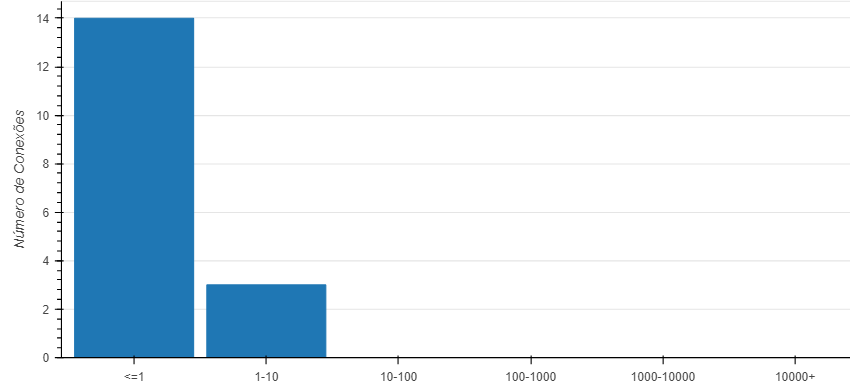
\includegraphics[scale=0.5]{images/colab_users_by_connection.png}
\end{figure}

Percebe-se que cerca de 83\% dos usuários possuem até 10 conexões, considerando-se a soma de seguidores e pessoas seguidas. Esse valor pode parecer baixo em comparação com outras redes sociais mais populares. No entanto, é importante ressaltar que cada plataforma possui suas particularidades e caberia aprofundar, em estudos futuros, a principal motivação dos usuários para estabelecerem conexões entre si. É possível que muitos usuários busquem se conectar com pessoas conhecidas em seu cotidiano, mas também pode haver usuários que possuam maior influência devido ao seu perfil de uso do aplicativo, por exemplo. Para compreender se há variações nos perfis de conexões em cada cidade, foram destacadas as informações de Mesquita, Niterói e Santo André.

De maneira geral, Niterói e Santo André apresentam comportamentos semelhantes, com melhor distribuição dos usuários nas faixas de 2-10 e 10-1000 conexões. Nessa última faixa, Niterói possui o maior percentual, com 14\%. Por outro lado, em Mesquita, prevalece a faixa de 1 conexão por usuário (53\%), o que pode indicar uma rede menos integrada (pelo menos em relação às conexões).

\begin{figure}[!htb]
	\caption{Distribuição das conexões entre os usuários de Mesquita, Niterói e Santo André}
	\label{fig:colab_users_by_connections_on_cities}
	\centering
	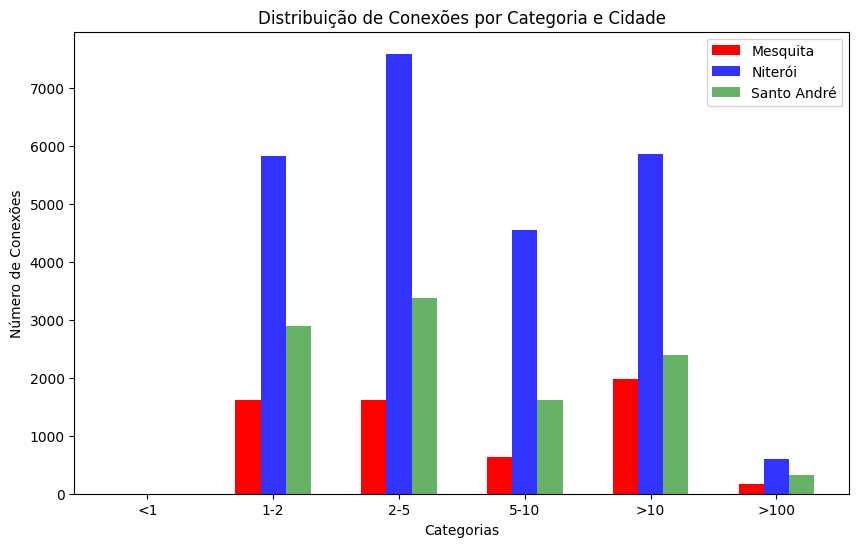
\includegraphics[scale=0.5]{images/colab_users_by_connections_on_cities.png}
\end{figure}

\subsection*{Apoios}

As curtidas no Colab são divididas em três grandes grupos: curtidas em publicações, comuniques ou propostas (que não existem mais). A plataforma conta com aproximadamente 1,5 milhão de curtidas, realizadas por um total de 100.265 usuários. Verifica-se que a maior parte das curtidas ocorre em publicações relacionadas à zeladoria, as quais representam o maior volume de atividades no feed. Em resumo, a média de curtidas por usuário é de 14, com uma mediana de 2 curtidas. Ao aprofundar a análise para o nível individual dos usuários, é possível constatar diferentes perfis, que variam de 1 até 51.966 curtidas. Apesar de alguns usuários apresentarem um comportamento discrepante, 85\% dos cidadãos realizaram até 10 curtidas. Ao analisar a participação nas três cidades selecionadas - Mesquita, Niterói e Santo André, não foram encontradas diferenças relevantes no percentual de curtidas.

\begin{figure}[!htb]
	\caption{Distribuição de curtidas ao longo dos anos}
	\label{fig:colab_likes_overtime}
	\centering
	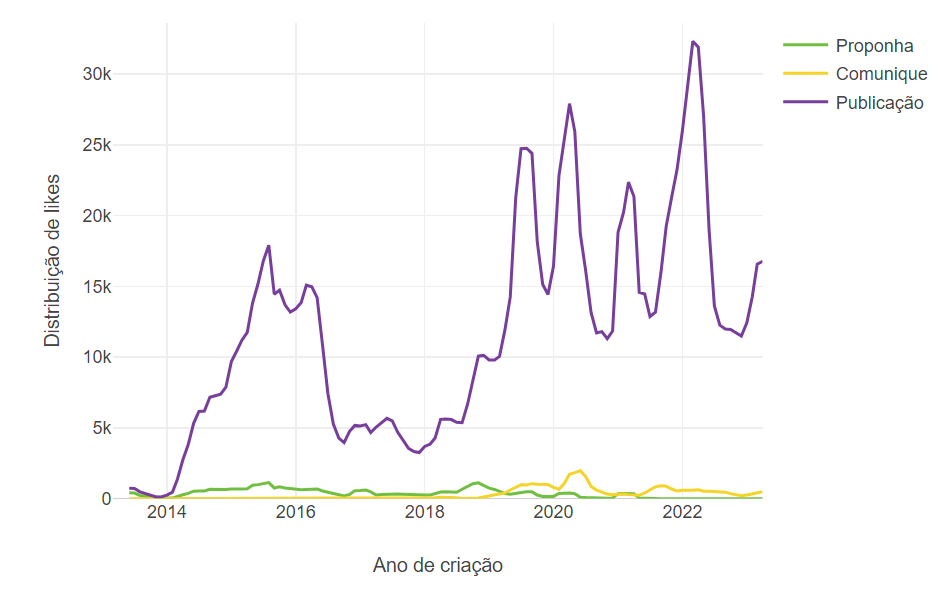
\includegraphics[scale=0.5]{images/colab_likes_overtime.png}
\end{figure}

\subsection*{Usuários com mais curtidas}

Ao analisar os usuários com maior número de curtidas, foram destacados os 1.000 usuários que mais curtiram. A faixa etária desses usuários varia entre 13 e 83 anos, com representantes de 62 cidades distintas. As cidades com maior número de representantes são Niterói, Teresina e Juiz de Fora. De maneira geral, predominam pessoas do gênero masculino (71\%), brancos (25\%), com ensino superior completo (35\%) e uma mediana de idade de 44 anos.

\subsection*{Comentários}

Ao analisar os comentários feitos pelos cidadãos, constatou-se a presença de 364.078 comentários até o momento, realizados por 60.452 usuários distintos. Dessa forma, obtemos uma média de 6 comentários por usuário e uma mediana de 2 comentários. O maior número de comentários realizados por um único usuário é de 13.875.Assim como nas conexões e curtidas, a grande maioria dos usuários concentra-se na realização de até 10 comentários.

\begin{figure}[!htb]
	\caption{Distribuição de comentários por idade}
	\label{fig:colab_comments_by_age}
	\centering
	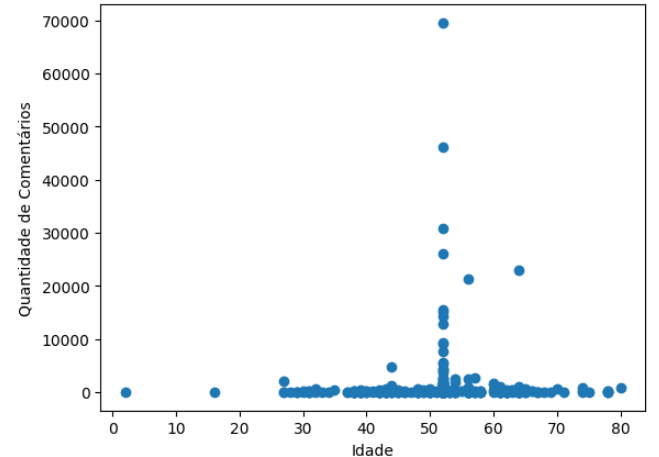
\includegraphics[scale=0.8]{images/colab_comments_by_age.png}
\end{figure}

Ao isolar as três cidades utilizadas como amostra nesse projeto, podem ser observados comportamentos distintos em cada uma. Nesse caso, Mesquita e Santo André apresentam comportamentos bastante semelhantes, com maior concentração dos usuários na faixa de 1-10 comentários. As três cidades possuem proporções similares nas faixas acima de 10 comentários.

\subsection*{Usuários com mais comentários}

Ao analisar os usuários com maior número de comentários, foram destacados os 1.000 usuários que mais comentam. A faixa etária desses usuários varia entre 16 e 84 anos, com representantes de 51 cidades distintas. As cidades com maior número de representantes são Niterói, Juiz de Fora e Santo André. De maneira geral, há predominância de homens (74\%), brancos (27\%), com ensino superior completo e uma mediana de idade de 45 anos.

\begin{figure}[!htb]
	\caption{Distribuição de Usuários por Quantidade de Comentários (por Cidade)}
	\label{fig:colab_comments_by_city}
	\centering
	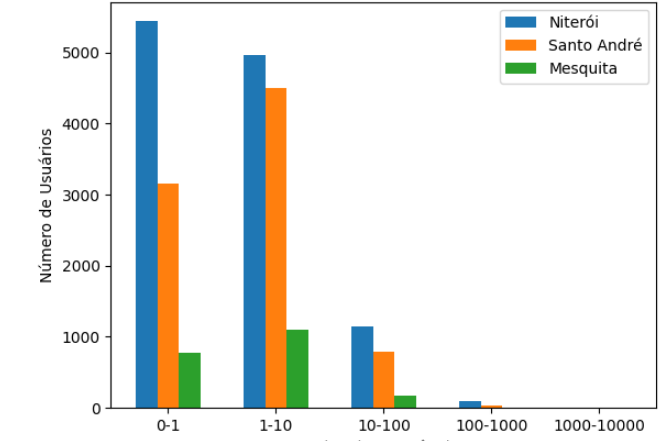
\includegraphics[scale=0.8]{images/colab_comments_by_city.png}
\end{figure}

\subsection*{Niterói, Mesquita e Santo André}

Para realizar análises mais aprofundadas, tanto de correlações quanto de análises de rede, foram selecionados os dados das três cidades com maior número de interações no Colab: Niterói, Santo André e Mesquita.

\subsection*{Correlação}

Com o objetivo de traçar um perfil dos usuários mais ativos na plataforma, buscou-se identificar alguma correlação entre a quantidade de atividades realizadas pelos cidadãos e suas principais características cadastrais (quando disponíveis). 

\begin{figure}[!htb]
	\caption{Matriz de Correlação}
	\label{fig:colab_correlation_matrix}
	\centering
	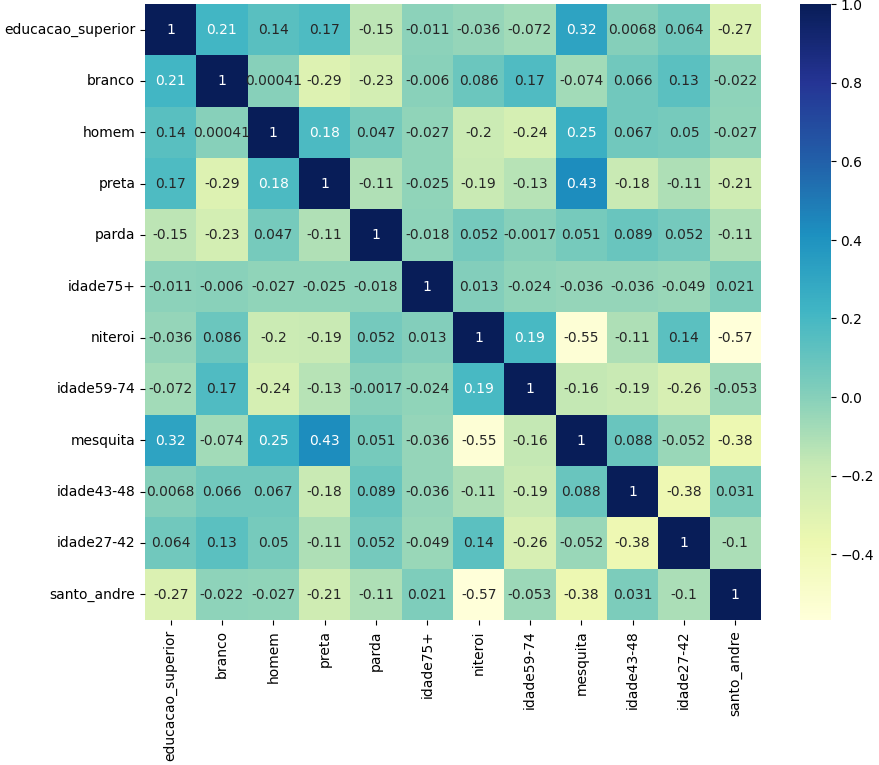
\includegraphics[scale=0.6]{images/colab_correlation_matrix.png}
\end{figure}

Para viabilizar a análise, algumas características foram transformadas em formato booleano (TRUE/FALSE). As características utilizadas foram:

\begin{itemize}
	\item Cidade do usuário, com destaque para Mesquita, Niterói e Santo André.
	\item Escolaridade, sendo considerado o nível "Superior +" que engloba ensino superior completo, mestrado e doutorado.
	\item Idade, com um recorte entre 10 e 90 anos e divisão em 5 faixas de tamanho igual: 10-26; 27-42; 43-58; 59-74; 75-90.
	\item Tipos de interações considerados para análise: comentários em publicações, curtidas em publicações, seguidores/seguindo e endosso ou rejeição de comentários .
	\item Cor/raça, incluindo as categorias branca, preta e parda.
	\item Gênero, considerando apenas homens.
	\item Número de interações acima da mediana do total de interações de cada usuário.
\end{itemize}

Com os dados disponíveis, não foi possível identificar características dos cidadãos que determinassem seu perfil de comportamento na plataforma. Portanto, não foram encontradas correlações relevantes para análise.

\begin{figure}[!htb]
	\caption{Matriz de Correlação}
	\label{fig:colab_correlation_bingo}
	\centering
	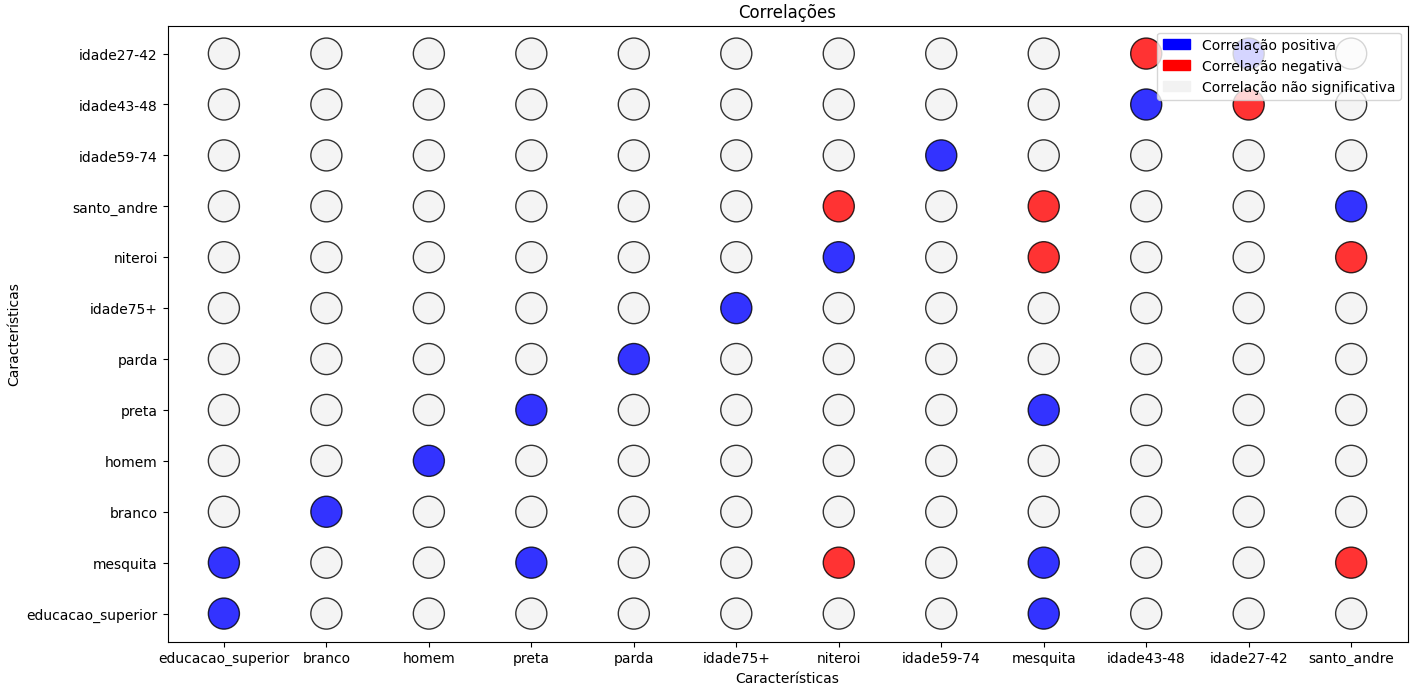
\includegraphics[scale=0.4]{images/colab_correlation_bingo.png}
\end{figure}

\subsection*{Regressão logística}

A fim de identificar características dos usuários que influenciam seu comportamento na plataforma, foi realizada uma regressão logística com base nas mesmas informações.

\begin{figure}[!htb]
	\caption{Regressão Logística}
	\label{fig:regression_chart}
	\centering
	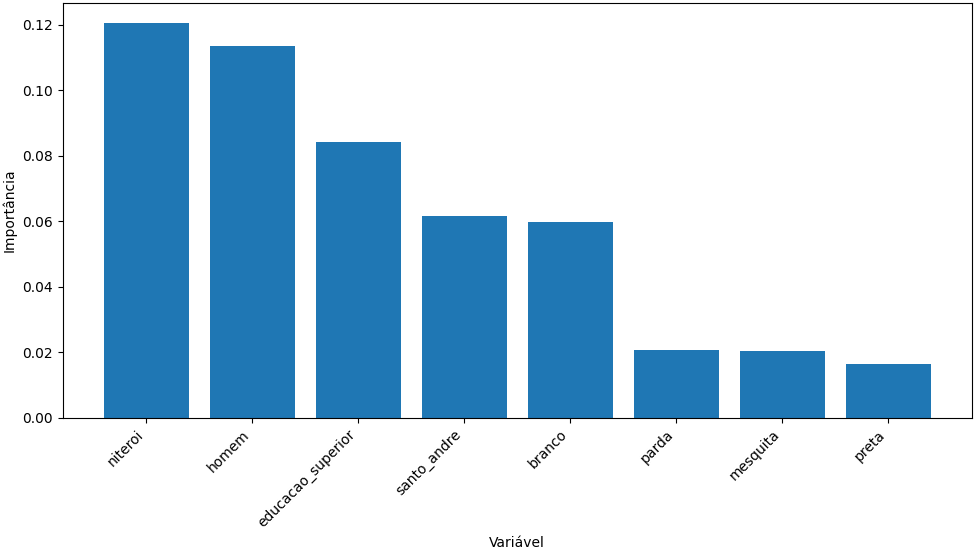
\includegraphics[scale=0.6]{images/regression_chart.png}
\end{figure}

A variável preditora utilizada foi o recorte no número de interações dos usuários: para aqueles que realizaram mais de 3 interações, ou seja, acima da mediana, foi atribuído o valor TRUE; para aqueles com interação menor que a mediana, FALSE.

A regressão logística apresentou uma AUC (área sob a curva ROC) baixa, indicando baixa precisão na previsibilidade das variáveis. No entanto, as variáveis preditoras mais relevantes foram:

\begin{itemize}
	\item Cidade de Niterói.
	\item Cor branca.
	\item Escolaridade compreendida entre ensino superior completo, mestrado e doutorado.
	\item Cor parda.
	\item Gênero masculino.
\end{itemize}

\begin{figure}[!htb]
	\caption{Regressão Logística - Curva ROC}
	\label{fig:regression_roc}
	\centering
	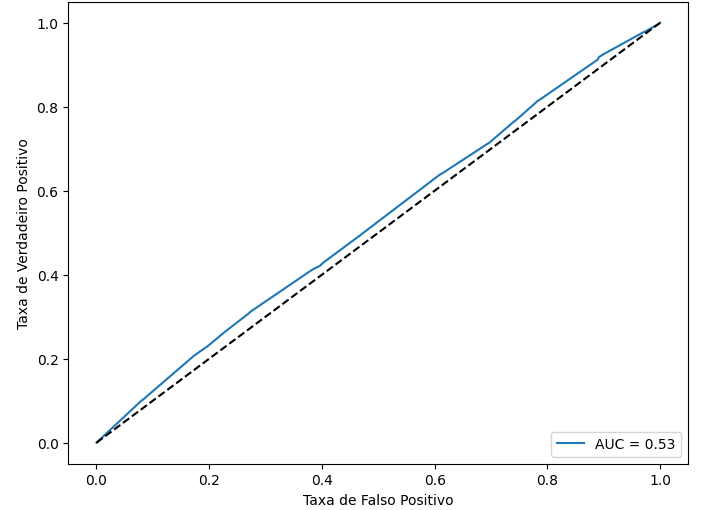
\includegraphics[scale=0.8]{images/regression_roc.png}
\end{figure}

\chapter{Fundamentação teórica}
\label{chapter:05_networkanalysis}
Neste capítulo, apresentamos os fundamentos da Análise de Redes Sociais. A análise de redes sociais (ARS) é uma abordagem que tem suas raízes na Sociometria e na Teoria dos Grafos, que são de viés matemático, para analisar relações sociais \cite{2015_Recuero_BOOK}. A ideia central é que os indivíduos, ou atores sociais, estão inseridos em estruturas complexas de relações com outros atores, e essas estruturas têm um papel fundamental no comportamento e na visão de mundo desses indivíduos.

\section{Teoria dos Grafos}
A Teoria dos Grafos é um framework matemático que estuda as relações entre objetos e as conexões entre eles. As origens desta teoria estão no trabalho de Euler e na solução que ele propôs para o enigma das Pontes de Königsberg. A história relata que a cidade de Königsberg seria atravessada por sete pontes e que popularmente havia um desafio de desenhar um caminho por ela onde cada uma das pontes seria atravessada uma única vez. Euler teria demonstrado que tal desafio era impossível de ser resolvido utilizando um grafo, dando assim origem à teoria.

Em \citeonline{2017_Recuero}, a autora discute a importância da ARS e da Teoria dos Grafos para a compreensão das redes sociais online. Ela explica que a ARS permite a análise sistemática de grupos sociais a partir de sua estrutura, através de medidas específicas. A autora também destaca que a análise de redes sociais nasce de um ramo interdisciplinar de pesquisa, cujas bases podem ser encontradas nas mais variadas ciências, principalmente no início do século XX, particularmente, a partir da década de 1930.

Um conceito fundamental na Teoria dos Grafos é o de um "grafo", que é uma estrutura composta por "vértices" (ou "nós") e "arestas" que conectam esses vértices. Formalmente, um grafo $G$ é definido como um par ordenado $G := (V, E)$ compreendendo um conjunto $V$ de vértices ou nós juntamente com um conjunto $E$ de arestas ou arcos, que são pares de vértices \cite{1976_Bondy_BOOK}.

Os grafos podem ser categorizados como direcionados ou não direcionados. Em um grafo direcionado, as arestas têm uma direção associada, indicando uma relação unidirecional. Em contraste, em um grafo não direcionado, as arestas não têm direção, sugerindo uma relação bidirecional \cite{2000_West_BOOK}. Em termos de redes sociais, um exemplo de grafo direcionado seria o Twitter (onde um usuário pode seguir outro sem ser seguido de volta), enquanto um exemplo de grafo não direcionado seria o Facebook (onde a amizade é sempre mútua).

\begin{figure}
	\centering
	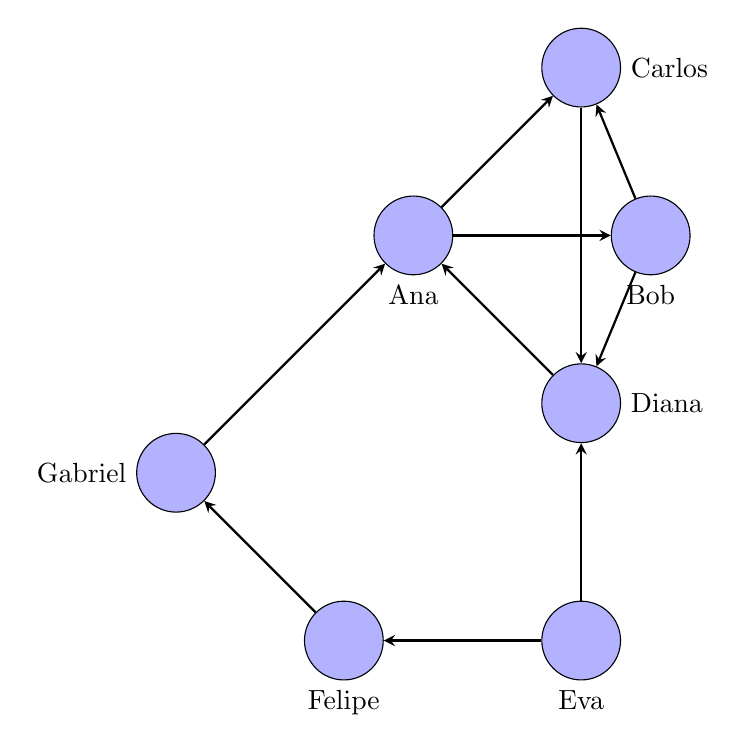
\begin{tikzpicture}[node distance=2cm]

		% Estilos para os nós e arestas
		\tikzstyle{user} = [circle, draw=black, fill=blue!30, minimum size=1cm, inner sep=0pt]
		\tikzstyle{follow} = [thick,->,>=stealth]

		% Usuários
		\node (A) [user, label=below:Ana] {};
		\node (B) [user, right=of A, label=below:Bob] {};
		\node (C) [user, above right=of A, label=right:Carlos] {};
		\node (D) [user, below right=of A, label=right:Diana] {};
		\node (E) [user, below=of D, label=below:Eva] {};
		\node (F) [user, left=of E, label=below:Felipe] {};
		\node (G) [user, above left=of F, label=left:Gabriel] {};

		% Relações de "seguir"
		\draw[follow] (A) -- (B);
		\draw[follow] (B) -- (C);
		\draw[follow] (C) -- (D);
		\draw[follow] (D) -- (A);
		\draw[follow] (A) -- (C);
		\draw[follow] (B) -- (D);
		\draw[follow] (E) -- (D);
		\draw[follow] (E) -- (F);
		\draw[follow] (F) -- (G);
		\draw[follow] (G) -- (A);

	\end{tikzpicture}
	\caption{Ilustração de uma rede social com usuários seguindo uns aos outros. O subgrafo formado por Ana, Bob, Carlos e Diana representa um clique, pois todos estão conectados entre si. O caminho de Eva para Ana passa por Diana e Gabriel.}
\end{figure}

Outro conceito importante é o "grau" de um vértice, que é o número de arestas conectadas a ele. Em um grafo direcionado, distinguimos entre o "grau de entrada" (o número de arestas que entram no vértice) e o "grau de saída" (o número de arestas que saem do vértice). O grau de um vértice pode ser usado para medir sua importância ou influência dentro da rede \cite{2010_Newman_BOOK}.

Um "caminho" em um grafo é uma sequência de vértices na qual cada vértice é conectado ao próximo por uma aresta. O "comprimento" de um caminho é o número de arestas que ele contém. Este conceito é crucial para entender como a informação ou influência pode se propagar através da rede \cite{2010_Easley_BOOK}.

A "conectividade" de um grafo é uma medida de quão integrada ou unida é a rede. Um grafo é dito "conectado" se houver um caminho entre cada par de vértices \cite{2000_West_BOOK}.

Um "subgrafo" é um grafo formado a partir de um conjunto de vértices e arestas de um grafo maior. Os subgrafos podem ser usados para estudar partes específicas de uma rede \cite{2000_West_BOOK}.

Recuero também enfatiza a diferença entre redes sociais e sites de rede social. Enquanto uma rede social está relacionada à percepção de um grupo social determinado pela sua estrutura (a “rede”), que é geralmente oculta, pois só está manifesta nas interações, as ferramentas sociais na internet são capazes de publicizar e influenciar essas estruturas sociais. Assim, o Facebook, por si só, não apresenta redes sociais. É o modo de apropriação que as pessoas fazem dele que é capaz de desvelar redes que existem ou que estão baseadas em estruturas sociais construídas por essas pessoas.

Portanto, a Teoria dos Grafos e a Análise de Redes Sociais são ferramentas essenciais para a compreensão das complexas redes de interações sociais que se formam tanto no mundo offline quanto online. Elas permitem uma visão mais profunda e sistemática das relações sociais, contribuindo para uma melhor compreensão dos fenômenos sociais.

\subsection*{Grafos Sociais}

Um dos primeiros desenvolvimentos na análise de redes foi o trabalho do sociólogo Georg Simmel no início do século XX. Simmel aplicou os princípios da teoria dos grafos às relações sociais, argumentando que as estruturas sociais surgem a partir dos padrões de interação entre os indivíduos \cite[]{2021_Hollstein}. Desde então, a análise de redes tem sido aplicada em uma ampla gama de campos, incluindo ciência da computação, física, biologia e ciências sociais, entre outros.

Simmel foi pioneiro em determinar a interação social como o bloco de construção básico da sociologia, indo além de seus contemporâneos, como Spencer. Ele argumentou que para entender o comportamento social, devemos estudar os padrões de interação, oferecendo insights penetrantes sobre a dinâmica das relações sociais. Embora Simmel nunca tenha usado o termo "rede social", muitos analistas de rede o consideram um precursor importante da abordagem de rede social.

Além disso, a análise de redes tem sido usada para entender a estrutura e a dinâmica de "redes escuras", como redes de criminosos ou terroristas. A análise de redes também tem sido aplicada para entender a estrutura e a dinâmica das organizações e como a estrutura da rede pode afetar a eficácia e a eficiência organizacional.

No entanto, apesar do rápido crescimento da análise de redes nas últimas duas décadas, as críticas à abordagem também aumentaram. Alguns críticos argumentam que a análise de redes pode ser excessivamente determinística, ignorando a agência individual e a complexidade das relações sociais \cite{1991_Scott}. Além disso, a análise de redes pode ser desafiadora devido à dificuldade de coletar dados completos e precisos sobre redes sociais.

A análise de redes sociais tem sido criticada por sua falta de consideração pelos aspectos qualitativos das redes sociais e por sua tendência a simplificar as complexidades das interações sociais \cite{2013_Gruzd}. Além disso, a análise de redes sociais é frequentemente criticada por sua falta de consideração pelos aspectos contextuais das redes sociais e por sua ênfase excessiva em padrões estruturais.

Essas críticas destacam a necessidade de abordagens mais holísticas e integradas para a análise de redes sociais, que levem em consideração tanto os aspectos quantitativos quanto qualitativos das redes sociais, bem como os contextos sociais e culturais em que essas redes estão inseridas.

A Teoria dos Grafos, nascida do problema das Pontes de Königsberg e formalizada por Euler, estabeleceu as bases para entendermos as complexas interconexões que permeiam não apenas estruturas físicas, mas também relações sociais. À medida que a sociedade evoluiu, as redes de interação humana se expandiram do tangível para o virtual, com as redes sociais online se tornando um novo território para aplicação desses princípios matemáticos.

O salto das pontes de Königsberg para os padrões de conexão no Twitter e Facebook não é apenas uma questão de escopo, mas também de complexidade. As redes sociais digitais de hoje permitem interações que Euler jamais poderia ter imaginado, mas a essência de sua abordagem permanece relevante. Assim como ele usou vértices e arestas para resolver o problema das pontes, hoje usamos esses mesmos elementos para mapear e entender a dinâmica das redes sociais.

Neste novo contexto, as interações entre usuários, as relações de seguimento e amizade, e até mesmo os padrões de compartilhamento de conteúdo podem ser modelados como grafos. As arestas representam as várias formas de interação — curtidas, comentários, retweets — e os vértices são os usuários, cada um com sua rede de conexões. Esta modelagem permite uma análise sofisticada do comportamento online, revelando desde estruturas de comunidade até a disseminação de informação e influência.

O estudo de grafos em redes sociais online transcende a análise de padrões de conexão. Abre-se a possibilidade de entender como as informações fluem, como as opiniões se formam e se polarizam, e como as comunidades online se organizam e interagem entre si. Portanto, ao aplicar a Teoria dos Grafos ao Colab, esta pesquisa busca desvendar não apenas a estrutura da rede, mas também o pulsar da participação cívica dentro dela, aplicando antigos conceitos matemáticos para resolver questões modernas de engajamento social e governança digital.

Para entender como essa disciplina pode ser aplicada ao Colab, é preciso primeiro entender o que é uma rede social online e como ela pode ser representada como um grafo. Em seguida, é preciso conhecer as principais métricas de análise de redes sociais e como elas podem ser usadas para entender o comportamento dos usuários. Por fim, é preciso entender como essas métricas podem ser aplicadas ao Colab para entender a dinâmica da participação cívica na plataforma. A seguir apresentamos algumas métricas derivativas importantes que podem ser calculadas a partir de uma lista de nós e arestas.

\subsection*{Modularidade}

\begin{figure}
	\centering
	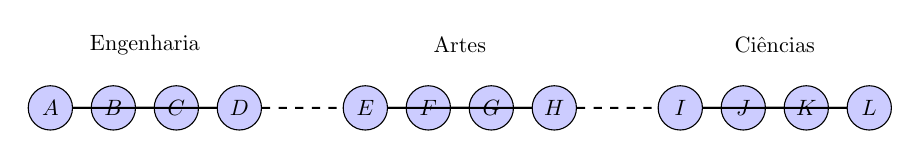
\begin{tikzpicture}[scale=0.8, every node/.style={scale=0.8}]
		% Styles
		\tikzstyle{vertex}=[circle,draw=black,fill=blue!20,minimum size=20pt,inner sep=0pt]
		\tikzstyle{edge}=[draw,thick,-]

		% Nodes for Engenharia
		\foreach \name/\x in {A/1,B/2,C/3,D/4}
		\node[vertex] (\name) at (\x,4) {$\name$};

		% Nodes for Artes
		\foreach \name/\x in {E/6,F/7,G/8,H/9}
		\node[vertex] (\name) at (\x,4) {$\name$};

		% Nodes for Ciências
		\foreach \name/\x in {I/11,J/12,K/13,L/14}
		\node[vertex] (\name) at (\x,4) {$\name$};

		% Connect nodes in Engenharia
		\foreach \source/\dest in {A/B, B/C, C/D, D/A, A/C, B/D}
		\path[edge] (\source) -- (\dest);

		% Connect nodes in Artes
		\foreach \source/\dest in {E/F, F/G, G/H, H/E, E/G, F/H}
		\path[edge] (\source) -- (\dest);

		% Connect nodes in Ciências
		\foreach \source/\dest in {I/J, J/K, K/L, L/I, I/K, J/L}
		\path[edge] (\source) -- (\dest);

		% Connect nodes between departments
		\path[edge, dashed] (D) -- (E);
		\path[edge, dashed] (H) -- (I);

		% Labels
		\node[align=center] at (2.5,5) {Engenharia};
		\node[align=center] at (7.5,5) {Artes};
		\node[align=center] at (12.5,5) {Ciências};
	\end{tikzpicture}
	\caption{Ilustração da modularidade em uma rede de estudantes de diferentes departamentos. Os nós representam estudantes, as arestas sólidas representam interações dentro dos departamentos e as arestas tracejadas representam interações entre departamentos.}
\end{figure}

A modularidade é uma métrica que quantifica a estrutura de comunidades em redes. Introduzida por \cite{2004_Newman}, a modularidade mede a diferença entre a fração de arestas que caem dentro de comunidades e a fração esperada se as arestas fossem distribuídas ao acaso, mantendo a distribuição de grau dos nós. Valores de modularidade próximos a 0 indicam que a divisão da rede em comunidades não é melhor do que uma atribuição aleatória, enquanto valores próximos a 1 indicam uma divisão forte em comunidades. Em termos práticos, uma rede com alta modularidade tem mais conexões dentro de suas comunidades e menos conexões entre comunidades diferentes do que seria esperado por acaso.

Para ilustrar, imagine uma rede social de estudantes de uma universidade, onde os estudantes pertencem a diferentes departamentos, como Engenharia, Artes e Ciências. Se os estudantes de Engenharia tendem a interagir mais frequentemente entre si, e o mesmo acontece com os estudantes de Artes e Ciências, então essa rede teria uma alta modularidade. Isso porque há uma densidade maior de conexões dentro de cada departamento (comunidade) do que entre departamentos diferentes. Em contraste, se os estudantes interagissem aleatoriamente, independentemente de seus departamentos, a modularidade seria próxima de 0, indicando uma ausência de estrutura comunitária clara.

\subsection*{Centralidade e Comunidades}

Um método comum usado na análise de redes é a análise de centralidade, que mede a importância dos nós na rede com base em sua posição e conexões dentro da rede \cite[]{1978_Freeman}. Medidas de centralidade podem ajudar a identificar atores-chave na rede, ou nós que desempenham papéis importantes como porteiros, conectores ou intermediários entre diferentes partes da rede.

Outro método importante na análise de redes é a detecção de comunidades, que identifica grupos de nós que estão mais densamente conectados entre si do que com o restante da rede \cite[]{2004_Newman}. A detecção de comunidades pode ajudar a identificar grupos de indivíduos com atributos ou comportamentos semelhantes, ou grupos que são mais suscetíveis à propagação de informações ou influências.

\subsection*{Algoritmo de Louvain}

A partir dos conceitos de centralidade, comunidade e modularidade, é possivel criar heurísticas mais especializadas para interpretar os grafos das redes, por exemplo, o algoritmo de Louvain é uma metodologia heurística para detecção de comunidades em grandes redes. Desenvolvido por \citeonline{2008_Blondel}, o algoritmo tem como principal objetivo identificar grupos de nós em redes que estão mais densamente conectados entre si do que com o restante da rede. A ideia central é maximizar a modularidade da forma mais eficiente possível.

O algoritmo opera em duas fases que são repetidas iterativamente. Na primeira fase, cada nó é atribuído à sua própria comunidade. Em seguida, para cada nó, o algoritmo avalia a ganho de modularidade ao mudar a comunidade desse nó para a comunidade de seus vizinhos. Se um aumento na modularidade é observado, o nó é colocado na comunidade que proporciona esse aumento. Este processo é repetido para todos os nós até que nenhum aumento na modularidade possa ser alcançado. Na segunda fase, as comunidades encontradas na primeira fase são agregadas para formar uma nova rede de comunidades, onde os nós da nova rede representam as comunidades e os links representam as conexões entre comunidades da rede original. Estas duas fases são repetidas até que a modularidade se estabilize.

No contexto de estudos sobre câmaras de eco, o algoritmo de Louvain é particularmente relevante. Câmaras de eco são, por definição, grupos de indivíduos que compartilham e reforçam opiniões semelhantes, minimizando a exposição a opiniões divergentes. A capacidade do algoritmo de Louvain de identificar comunidades densamente conectadas em redes torna-o uma ferramenta valiosa para detectar esses grupos. Ao identificar comunidades que interagem predominantemente entre si, os pesquisadores podem isolar e estudar essas câmaras de eco, compreendendo melhor sua formação, evolução e impacto na disseminação de informações.

\section{Aplicações da Análise de Redes}

A análise de redes tem sido aplicada em uma ampla gama de campos, além das redes sociais, com aplicações que vão desde redes de transporte até a neurociência. Nesta seção, vamos destacar algumas contribuições notáveis.

No campo do transporte, a análise de redes tem sido usada para estudar o fluxo de tráfego nas estradas e identificar áreas de gargalo que podem ser melhoradas para aumentar a eficiência do tráfego \cite[]{2012_Levinson}. Por exemplo, \citeonline{2010_Bierlaire} aplicaram a análise de redes para otimizar o sistema de transporte público, reduzindo o tempo de viagem e melhorando a eficiência do serviço. No campo acadêmico, a análise de redes tem sido aplicada para estudar as redes de coautoria na publicação acadêmica. \citeonline{2001_Newman} utilizou a análise de redes para estudar os padrões de colaboração entre autores e a emergência de comunidades de pesquisa. No campo organizacional, a análise de redes tem sido usada para compreender a estrutura de padrões de comunicação formais e informais em organizações. \citeonline{2004_Cross_BOOK} utilizaram a análise de redes para entender como os indivíduos influenciam os processos de tomada de decisão e a emergência de estruturas de poder dentro das organizações. Na biologia, a análise de redes tem sido usada para estudar redes de interação de proteínas, redes regulatórias de genes e redes metabólicas \citeonline{2004_Barabasi} utilizaram a análise de redes para entender como as proteínas interagem entre si em uma célula, fornecendo insights sobre como as doenças afetam essas interações.
\begin{figure}[!htb]
	\caption{Imagem ilustrativa de uma rede de interação de proteínas}
	\label{fig:network_proteins}
	\centering
	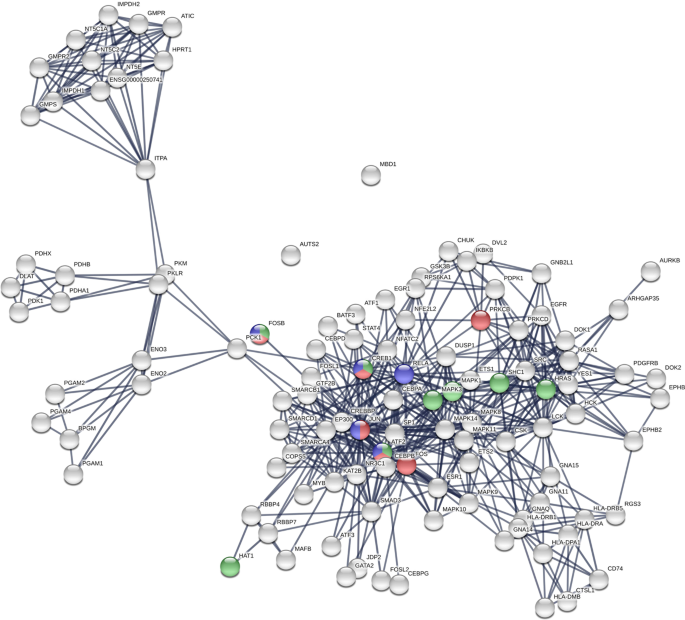
\includegraphics[scale=0.5]{network_proteins.png}
	\fdireta{2004_Barabasi}
\end{figure}
A análise de redes também tem sido usada em neurociência para estudar redes cerebrais. Por exemplo, pesquisadores têm utilizado a análise de redes para entender como diferentes regiões do cérebro interagem entre si, o que pode ajudar a entender doenças como a esquizofrenia e o Alzheimer \cite[]{2009_Bullmore}.
\begin{figure}[!htb]
	\caption{Imagem ilustrativa de uma rede de interação de proteínas}
	\label{fig:network_brain}
	\centering
	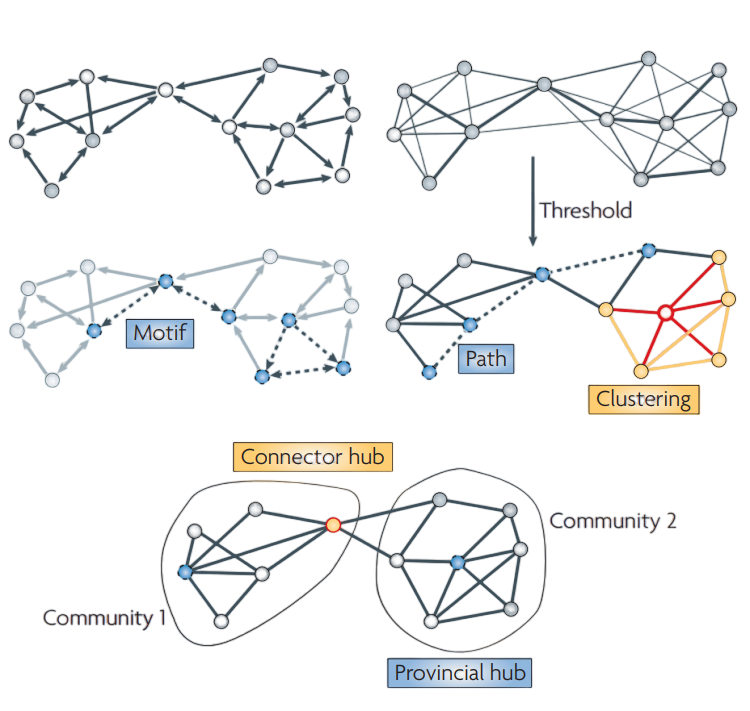
\includegraphics[scale=0.25]{network_brain.png}
	\fdireta{2009_Bullmore}
\end{figure}

\subsection*{Análise de Redes Sociais Online}

Outra importante aplicação da análise de redes está no estudo de comunidades online e mídias sociais. O crescimento exponencial de plataformas online e redes sociais tem fornecido aos pesquisadores vastas quantidades de dados para analisar a dinâmica dessas comunidades. Por exemplo, um estudo de utilizou a análise de redes para investigar a estrutura e dinâmica das comunidades de discussão online no Reddit. O estudo constatou que as comunidades exibiam uma estrutura hierárquica com subcomunidades distintas que se formavam em torno de tópicos específicos. Outro estudo de \citeonline{2011_Quercia_IP} utilizou a análise de redes para estudar a influência de relacionamentos sociais na propagação de informações no Twitter. O estudo constatou que a estrutura da rede social influenciava a propagação de informações, sendo que clusters densamente conectados tinham maior probabilidade de promover a difusão de informações do que clusters esparsamente conectados.

Esse tópico buscou demonstrar como a análise de redes é uma ferramenta poderosa para analisar sistemas complexos e compreender as relações entre seus componentes. Ela tem suas origens na teoria dos grafos e se desenvolveu em um campo multidisciplinar com aplicações em várias áreas, como redes sociais, comunidades online, epidemiologia, ecologia e transporte. A aplicação da análise de redes em redes sociais tem levado a insights importantes sobre a estrutura e dinâmica dessas redes e tem ajudado os pesquisadores a compreender os mecanismos de influência social e a propagação de informações. O uso da análise de redes em outros campos também tem levado a descobertas importantes e tem o potencial de aprimorar nossa compreensão dos sistemas que moldam nosso mundo.

\subsection*{Análise de Redes Sociais no Brasil}

A Análise de Redes Sociais (ARS) emergiu como uma ferramenta poderosa e cada vez mais popular para analisar a estrutura e a dinâmica das redes sociais. Utilizada para estudar uma variedade de fenômenos, como comportamento organizacional, redes políticas, crime e inovação, a ARS tem demonstrado ser uma metodologia extremamente versátil. No Brasil, a relevância da ARS é evidenciada em múltiplos contextos e áreas de estudo, incluindo o planejamento urbano, a avaliação de políticas públicas, a compreensão das dinâmicas de migração e a análise de preconceitos e divisões sociais nas redes sociais.

Um dos aspectos que torna a ARS especialmente relevante no Brasil é o alto uso de redes sociais pela população. O Brasil é um dos países com maior número de usuários de redes sociais no mundo, criando um vasto campo de dados que pode ser analisado através da ARS. Além disso, a diversidade cultural e regional do Brasil, com suas muitas diferenças locais, proporciona um cenário complexo que a ARS pode ajudar a decifrar. Ao identificar padrões de interação e circulação de informações nas redes sociais, a ARS pode revelar como essas diferenças regionais e culturais se manifestam online.

Além disso, o Brasil enfrenta uma série de questões sociais complexas e uma alta polarização política, aspectos que são frequentemente expressos e amplificados nas redes sociais. A ARS pode ser uma ferramenta valiosa para entender a formação e a dinâmica dessas polarizações, assim como para estudar a formação de grupos de opinião e a disseminação de informações (ou desinformação). Por último, eventos de grande escala, como a Copa do Mundo, as Olimpíadas ou as eleições presidenciais, geram uma enorme quantidade de atividade nas redes sociais, proporcionando oportunidades únicas para a aplicação da ARS.

Diante deste cenário, este capítulo apresenta um resumo breve da de algumas contribuições relevantes que utilizam a ARS no Brasil, começando com uma revisão de suas principais contribuições teóricas e metodológicas. Em seguida, ele discute os desafios atuais e futuros na aplicação desta abordagem no contexto brasileiro, com o objetivo de explorar como a ARS pode continuar a fornecer insights valiosos em meio à constante evolução das redes sociais.

Do ponto de vista teórico, a Análise de Redes Sociais (ARS) tem sido fundamental para entender como as redes sociais influenciam a formação de opiniões, a disseminação de informações e a mobilização social. Um exemplo relevante é o estudo de \citeonline{2021_Recuero}, que investigaram a polarização em torno do uso da cloroquina para tratar a COVID-19 no Brasil, analisando dados do Twitter. O estudo mostrou como a ARS pode ser aplicada para identificar câmaras de eco e a formação de bolhas de filtro, onde usuários com diferentes posições políticas e ideológicas têm acesso a fontes de informação divergentes. A análise revelou que a narrativa sobre a cloroquina foi capturada pela disputa política, com diferentes grupos compartilhando e reforçando suas crenças por meio das redes sociais. O trabalho de Recuero também informa a metodologia de \citeonline{2021_Kalinke} que explora a topologia da rede entre usuários do Twitter apoiadores e críticos ao governo de Jair Bolsonaro em relaçao as 100 mil mortes por COVID-19. O estudo utilizou métricas de centralidade para identificar clusters de usuários que não interagem entre membros fora das suas bolhas, o que contribui com um discurso reverberado por câmaras de eco.

Além disso, a ARS tem sido usada para investigar como as redes sociais podem facilitar a disseminação de informações falsas ou enganosas, o que tem implicações significativas para a democracia e a saúde pública. Um estudo interessante foi conduzido por \citeonline{2020_Lima}, que analisaram a circulação de informações sobre a COVID-19 no Twitter. Eles utilizaram a ARS para identificar padrões de compartilhamento de conteúdo e relacionamentos entre usuários. O estudo revelou que a desinformação estava fortemente associada ao consumo de veículos hiperpartidários e ao conteúdo de mídia social, enquanto a informação factual estava mais associada a veículos jornalísticos e institucionais. Isso demonstra como a ARS pode contribuir para a compreensão dos mecanismos de propagação da desinformação nas redes sociais e auxiliar na identificação de estratégias para mitigar esse problema.

Outro estudo relevante é o de \citeonline{2015_Coelho}, que analisou a rede de interações no Twitter durante o \#ProtestodosPintas em Natal (RN). O estudo encontrou que os significados construídos nas redes sociais sobre o protesto foram em grande parte negativos, com a rede sendo articulada em torno de 2 perfis. Este estudo demonstra como a ARS pode ser usada para analisar a opinião pública e a formação de consenso (ou dissensão) em torno de eventos específicos.

Esses exemplos ilustram como a ARS tem contribuído para avanços teóricos e metodológicos na compreensão das redes sociais no contexto brasileiro. As aplicações da ARS mencionadas nos estudos citados fornecem insights valiosos sobre a formação de opiniões, a disseminação de informações, a polarização política e a estrutura das redes sociais em diferentes contextos. Ao utilizar técnicas da ARS e analisar os dados específicos desses estudos, os pesquisadores foram capazes de desvendar padrões, identificar comunidades e compreender as interações sociais e políticas nas redes sociais.

Finalmente, a diversidade cultural e regional do Brasil apresenta um desafio adicional. Como mencionado anteriormente, o Brasil é um país de grande diversidade, com muitas diferenças locais. Isso significa que a análise de redes sociais no Brasil deve levar em consideração essa diversidade, adaptando-se às especificidades de diferentes contextos regionais e culturais.

Com base nos dados extremamente localizados do Colab, nos quais os usuários interagem e criam eventos relacionados a problemas específicos em suas cidades, como buracos nas vias, calçadas irregulares, descarte irregular de lixo, vazamentos de água e iluminação pública, é possível obter insights valiosos tanto no âmbito social quanto político.

Em termos sociais, a análise das interações e dos padrões de engajamento dos usuários pode revelar informações sobre a coesão social e a formação de grupos de interesse em nível local. Por exemplo, ao examinar as postagens sobre problemas específicos, como buracos nas vias, é possível identificar redes de interação entre os usuários que compartilham preocupações semelhantes. Essas redes podem revelar comunidades de interesse e fornecer insights sobre a participação cívica local e a busca de soluções colaborativas para questões cotidianas.

Do ponto de vista político, a análise das interações políticas no Colab pode fornecer informações sobre a polarização e a formação de grupos de opinião em nível local. Por exemplo, ao examinar as postagens relacionadas a políticas públicas, é possível identificar padrões de interação entre usuários com diferentes posições políticas. Esses padrões podem ajudar a compreender a dinâmica da polarização política em nível local e como isso influencia a deliberação pública e a tomada de decisões políticas.

A análise dos dados do Colab sob uma perspectiva da ARS permite adquirir insights valiosos em diversos aspectos sociais e políticos, desde a coesão social em nível local até a dinâmica da polarização política. Ao estabelecer essas conexões, é possível obter uma compreensão mais abrangente e contextualizada das redes sociais e de como elas impactam a vida cotidiana e a tomada de decisões nas comunidades.

\section{Compreendendo Câmaras de Eco e suas implicações}
\label{05_echochambers}
As mídias sociais revolucionaram a forma como as pessoas se comunicam e interagem umas com as outras. No entanto, o lado negativo dessa revolução é a crescente polarização e isolamento das pessoas em câmaras de eco. Uma câmara de eco pode ser definida como um sistema fechado em que as pessoas interagem apenas com aquelas que compartilham das mesmas crenças, valores e ideologias, enquanto ignoram ou suprimem ativamente pontos de vista opostos \cite[]{2015_Bakshy}. O termo "câmara de eco" tem origem no conceito de uma câmara de reverberação sonora, onde as ondas sonoras são refletidas entre as paredes, amplificando e distorcendo o som original.

Câmaras de eco podem ter sérias implicações para a sociedade, pois limitam a exposição a perspectivas diversas, levando ao reforço de crenças existentes e à exclusão de pontos de vista alternativos \cite[]{2001_Sunstein_BOOK}. Isso pode contribuir para a criação de uma divisão ideológica, que pode prejudicar o diálogo construtivo e o compromisso, resultando em uma sociedade polarizada e fragmentada. Além disso, câmaras de eco podem levar à disseminação de desinformação, propaganda e notícias falsas, uma vez que os indivíduos dentro desses sistemas fechados têm menos probabilidade de verificar a veracidade das informações que corroboram suas crenças existentes \cite[]{2016_Vicario}.

Compreender os mecanismos por trás da formação e manutenção das câmaras de eco é crucial para lidar com as consequências negativas associadas a esses fenômenos. A formação de câmaras de eco pode ser atribuída a diversos fatores, incluindo os algoritmos utilizados pelas plataformas de mídias sociais, os vieses cognitivos dos indivíduos e a influência de líderes de opinião \cite[]{2016_Flaxman}.

Em termos de fatores algorítmicos, as plataformas de mídias sociais utilizam algoritmos personalizados que visam fornecer aos usuários conteúdo alinhado com seus interesses, crenças e preferências. Isso significa que os indivíduos têm maior probabilidade de serem expostos a conteúdos que reforçam suas crenças e valores existentes, levando à formação de câmaras de eco \cite[]{2015_Bakshy}.

Vieses cognitivos, como viés de confirmação e exposição seletiva, também podem contribuir para a formação de câmaras de eco, pois os indivíduos tendem a buscar informações que confirmam suas crenças pré-existentes, enquanto ignoram ou rejeitam informações que as desafiam \cite[]{2006_Taber}. Além disso, líderes de opinião ou indivíduos com alta influência social podem desempenhar um papel na formação e manutenção das câmaras de eco, pois podem moldar as crenças e atitudes de seus seguidores \cite[]{2015_Bakshy}.

Câmaras de eco são um fenômeno preocupante nas mídias sociais, pois podem levar à polarização e fragmentação da sociedade, além da disseminação de desinformação e propaganda. Compreender os mecanismos por trás da formação e manutenção das câmaras de eco é crucial para mitigar suas consequências negativas.

\section{Modelagem Baseada em Agentes}
A Modelagem Baseada em Agentes (MBA) é uma abordagem de modelagem computacional que permite simular e analisar sistemas complexos através da interação de agentes autônomos. Essa abordagem tem sido aplicada em diversos campos, como ciências sociais, economia, ecologia e engenharia, devido à sua capacidade de capturar comportamentos emergentes e padrões coletivos resultantes das interações entre os agentes.

No contexto específico das simulações de câmaras de eco, a MBA oferece uma poderosa ferramenta para investigar e compreender a dinâmica desses sistemas. As câmaras de eco são ambientes onde grupos de indivíduos compartilham e são expostos principalmente a informações e opiniões que confirmam suas crenças existentes, resultando em polarização e reforço de pontos de vista extremos. Utilizando a MBA, é possível modelar os usuários como agentes autônomos, considerando suas opiniões individuais, influências externas e interações em uma rede social.

Ao simular a interação e a propagação de informações entre os agentes, é possível estudar como as câmaras de eco se formam e evoluem, analisando os fatores que contribuem para a polarização e a formação de bolhas de informação. A MBA permite investigar diferentes estratégias de atualização de opinião dos agentes, a influência dos vizinhos na rede social e outros fatores que afetam a dinâmica das câmaras de eco. Além disso, é possível utilizar medidas e métricas para avaliar o impacto das câmaras de eco, como a diversidade de opiniões, a polarização e a exposição a diferentes perspectivas.

Portanto, a Modelagem Baseada em Agentes é uma valiosa ferramenta para compreender e analisar as dinâmicas das câmaras de eco. Ao simular a interação dos agentes em um ambiente controlado, é possível obter insights sobre os processos subjacentes e os efeitos resultantes das câmaras de eco. Essa abordagem permite explorar estratégias de mitigação e intervenção para promover a diversidade de opiniões e evitar o reforço de extremos, contribuindo para uma sociedade mais plural e informada.

Exploramos a metodologia proposta por Atiqi, focando na simulação da dinâmica de opiniões em uma rede social. O modelo de simulação é baseado em agentes, onde cada agente representa um usuário na rede social. Cada usuário possui uma opinião e uma exposição, que são atualizadas com base nas notícias que encontram e nas opiniões de seus vizinhos na rede.

A opinião de um usuário é um valor entre -1 e 1, representando o sentimento do usuário em relação a um determinado tópico. A exposição de um usuário é uma medida da diversidade de sentimentos das notícias que encontraram. Ela aumenta sempre que um usuário encontra uma notícia cujo sentimento é diferente de sua opinião atual.

O modelo de simulação utiliza diferentes estratégias para atualizar as opiniões dos usuários. A estratégia básica atualiza a opinião de um usuário com base no sentimento de uma notícia, se a diferença entre a opinião do usuário e o sentimento da notícia estiver abaixo de um determinado limite. Estratégias mais complexas também levam em consideração as opiniões dos vizinhos do usuário na rede. Por exemplo, a estratégia de Influência do Vizinho atualiza a opinião de um usuário em direção à opinião média de seus vizinhos se suas opiniões tiverem o mesmo sinal. A estratégia de Influência do Vizinho Ponderada faz o mesmo, mas pondera as opiniões dos vizinhos pela centralidade do eigenvector na rede.

Estratégia \texttt{NeighborInfluenceOpinionUpdateStrategy}:
\begin{equation*}
	O_i = O_i + \alpha \times (M_i - O_i)
\end{equation*}

em que:

\begin{itemize}
	\item $O_i$ representa a opinião do usuário $i$;
	\item $M_i$ representa a média das opiniões dos vizinhos do usuário $i$;
	\item $\alpha$ é o fator de influência que determina o quanto a opinião dos vizinhos influencia a opinião do usuário.
\end{itemize}

Estratégia \texttt{WeightedNeighborInfluenceOpinionUpdateStrategy}:
\begin{equation*}
	O_i = O_i + \alpha \times (M_{\text{ponderada}_i} - O_i)
\end{equation*}

em que:

\begin{itemize}
	\item $O_i$ representa a opinião do usuário $i$;
	\item $M_{\text{ponderada}_i}$ representa a média ponderada das opiniões dos vizinhos do usuário $i$;
	\item $\alpha$ é o fator de influência que determina o quanto a opinião ponderada dos vizinhos influencia a opinião do usuário.
\end{itemize}

A simulação produz várias métricas que podem ser usadas para analisar a dinâmica da rede:

\begin{itemize}
	\item Coeficiente Global de Câmaras de Eco (GEC): uma medida que quantifica a polarização de opiniões na rede. O GEC é calculado somando o produto das opiniões dos pares de usuários conectados por uma aresta na rede. Um valor positivo indica uma tendência de polarização, onde usuários com opiniões semelhantes estão mais propensos a se conectar entre si, enquanto um valor negativo indica uma tendência de diversidade de opiniões.
	\item Coeficiente de Câmaras de Eco de Exposição (ECC): uma medida que avalia a polarização de opiniões com base na diversidade de exposição a diferentes perspectivas. O ECC é calculado para cada usuário, considerando as opiniões dos seus vizinhos na rede. Um valor alto de ECC indica que um usuário está principalmente exposto a opiniões semelhantes à sua, refletindo a existência de câmaras de eco.
	\item Opinião Média: uma medida que representa a opinião média dos usuários na rede. É calculada como a média das opiniões individuais de todos os usuários. A opinião média fornece uma visão geral do sentimento coletivo em relação a um determinado tópico na rede.
	\item Exposição Média: uma medida que representa a exposição média dos usuários a diferentes perspectivas na rede. É calculada como a média das exposições individuais de todos os usuários. A exposição média reflete a diversidade de informações a que os usuários estão expostos e pode indicar o grau de pluralismo de opiniões na rede.
\end{itemize}

Considerando as heurísticas propostas em um contexto de simulação e as condições únicas dos dados do Colab, representando tanto uma topologia de grafo de rede social quanto o conteúdo produzido por usuários dessa rede, metodologia de Atiqi fornece um framework poderoso para simular e analisar a dinâmica de opiniões no Colab. O modelo baseado em agentes permite uma representação detalhada dos usuários e suas interações, enquanto as diversas métricas e visualizações proporcionam insights sobre a dinâmica da rede. No entanto, interpretar esses resultados de maneira significativa muitas vezes requer compará-los a outros resultados, seja de outras simulações ou de dados do mundo real. Nossa intenção é adaptar a metodologia de Atiqi para o caso de uso do Colab, substituindo as notícias por eventos reportados pelos usuários e as opiniões por sentimentos expressos nos comentários/postagens. Dessa forma, poderemos simular a dinâmica de opiniões e a formação de câmaras de eco no contexto do aplicativo Colab. Exploramos essas dinâmicas no \autoref{chapter:08_echochamberdetection}.

\section{Conclusões}
Neste capítulo de Fundamentação Teórica, exploramos conceitos e teorias essenciais que fornecem uma base sólida para a compreensão das dinâmicas das câmaras de eco em redes sociais, com foco na aplicação desses conceitos ao contexto do aplicativo Colab. Começamos introduzindo a teoria dos grafos e sua relevância na representação de redes sociais, destacando a importância da detecção de comunidades e da modularidade para identificar estruturas significativas dentro dessas redes. Em seguida, discutimos o algoritmo Louvain, uma técnica eficaz para a detecção de comunidades em redes complexas, que desempenhará um papel fundamental em nossas análises.

Em seguida, investigamos as aplicações da análise de redes sociais em diversos campos, reconhecendo a importância dessa abordagem na compreensão das dinâmicas das redes e na identificação de padrões emergentes. Exploramos as câmaras de eco e suas implicações nas mídias sociais, destacando como esses fenômenos podem levar à polarização e à disseminação de desinformação.

Examinamos as implicações negativas das câmaras de eco, incluindo a dificuldade de diálogo construtivo, a disseminação de desinformação e a fragmentação da sociedade. Investigamos os mecanismos por trás da formação das câmaras de eco, que envolvem algoritmos de personalização de conteúdo, vieses cognitivos e influência de líderes de opinião.

Destacamos a importância de compreender esses mecanismos para mitigar os efeitos negativos das câmaras de eco, especialmente no contexto do aplicativo Colab. Analisamos estudos relevantes que examinaram câmaras de eco em diferentes contextos, incluindo política climática e debates sobre vacinação.

Finalmente, introduzimos a Modelagem Baseada em Agentes (MBA) como uma ferramenta poderosa para simular a dinâmica das câmaras de eco. A MBA permite a criação de simulações que representam a interação de agentes autônomos, que são os usuários de redes sociais. Exploramos um modelo de simulação baseado em MBA que pode ser adaptado ao contexto do Colab, permitindo-nos investigar como as câmaras de eco podem se formar e evoluir dentro da plataforma.

No próximo capítulo, daremos um passo adiante na nossa jornada de compreensão das câmaras de eco no aplicativo Colab. Usando a poderosa ferramenta Gephi, realizaremos uma análise exploratória da rede do Colab. Iremos visualizar e examinar a estrutura da rede, identificar comunidades e padrões de interação, e começar a descobrir insights sobre como as câmaras de eco podem estar se formando na plataforma. Esta análise nos proporcionará uma base sólida para investigações mais aprofundadas e a formulação de estratégias para lidar com os desafios das câmaras de eco no Colab.

\chapter{Análise exploratória da Rede do Colab}
\label{chapter:06_exploratory}
Neste capítulo, apresentamos a criação de um grafo da rede social do Colab com base na fonte de dados disponibilizada pela empresa. O conjunto de dados consiste em uma lista de arestas, onde os nós representam os usuários e as arestas representam as conexões ou seguidores desses usuários. Utilizamos diversas técnicas de análise de redes, incluindo o agrupamento de Louvain, o agrupamento espectral e a centralidade de Eigenvector.

O agrupamento de Louvain é um algoritmo de detecção de comunidades que busca otimizar a modularidade, uma medida da densidade de conexões dentro das comunidades em comparação com as conexões entre as comunidades. Já o agrupamento espectral é uma técnica que utiliza os Eigenvectors do grafo para particionar os nós em comunidades. Além disso, exploramos a centralidade de Eigenvector para identificar os nós centrais na rede, ou seja, aqueles com maior influência ou importância. Essa medida utiliza os Eigenvectors para determinar a importância de um nó com base em sua conexão com outros nós na rede. Dessa forma, por meio dessas técnicas de análise de redes, buscamos compreender a estrutura e os padrões presentes na rede social do Colab.

Este estudo baseia-se em pesquisas anteriores que utilizaram a análise de redes para estudar redes sociais, como o Twitter e o Facebook, a fim de obter insights sobre a estrutura dessas comunidades. Por exemplo, \citeonline{2006_Newman} utilizaram o agrupamento espectral para identificar comunidades em uma rede de blogs políticos e mostraram que essas comunidades eram altamente polarizadas.

\subsection*{Pré-processamento do conjunto de dados Colab}
\label{sec:preprocessing}

Antes de carregar os dados em scripts e aplicações, realizamos algum pré-processamento nos arquivos CSV brutos usando a biblioteca Pandas do Python. O CSV original era uma lista de arestas em que a coluna "source" representava um usuário e a coluna "target" representava uma conexão com outro usuário. O arquivo CSV também tinha colunas para registrar quando essas relações foram criadas, atualizadas e excluídas, o que pode ser usado para adicionar dinâmica temporal à visualização. No entanto, os carimbos de data e hora originais estavam no formato brasileiro e precisaram ser convertidos para o formato ISO 8601, que é o padrão em SNA.

Outra etapa foi separar a tabela de arestas dos dados dos nós, dedicando um arquivo para as relações dos usuários expressas por meio das colunas "source" e "target", e outro arquivo para os dados dos nós dos usuários. Esses arquivos são edges.csv e nodes.csv, respectivamente. Neste momento, o arquivo de nós contém apenas dados temporais, mas mais adiante no experimento, pretendemos incorporar também dados de localização, por isso decidimos dividir os arquivos. Isso também é considerado um padrão mais consistente para carregar uma lista de arestas no em modelos baseados em grafos, conforme demonstrado por \citeonline{2016_Golbeck_PAGE}.

Também removemos nós duplicados. No contexto dos dados brutos, a coluna 'deleted\_at' representa quando um usuário foi deixado de seguir por outro usuário. Essa métrica nos fornece uma visão mais ampla do modelo de comunidade, mas, por simplicidade, optamos por removê-la deste primeiro experimento no Gephi. Retomaremos o estudo sobre a ação de deixar de seguir usuários posteriormente.

Para aproveitar o poder computacional, usamos o Google Colaboratory para realizar o pré-processamento dos dados. O script abaixo adapta as colunas de carimbos de data e hora e remove as linhas duplicadas.

\section{Construção de grafo da Rede Social}
A análise das interações dos usuários dentro do aplicativo Colab requer a criação de um grafo de rede social, a fim de representar visualmente as conexões entre os usuários e suas respectivas postagens. Dado que o banco de dados original do Colab é um banco de dados relacional, foi necessário realizar a transformação dos dados em uma estrutura de grafo.

A transformação dos dados de lista de arestas em uma estrutura de grafo permitiu uma representação mais adequada das relações e interações entre os usuários. Essa transformação envolveu a representação de cada usuário como um nó no grafo e a mapeamento das conexões entre os usuários como arestas.

Essa abordagem apresenta algumas vantagens importantes em relação à análise de redes sociais. Ao utilizar um formato de dados em grafo, foi possível visualizar e analisar a estrutura da rede de forma mais intuitiva, identificando grupos de usuários e suas interações com maior clareza. Além disso, a representação em grafo facilita a aplicação de algoritmos de análise de redes, como algoritmos de agrupamento e detecção de comunidades, que podem revelar informações relevantes sobre a estrutura da rede e a formação de câmaras de eco.

Essa estrutura de dados é obtida inicialmente no formato CSV, importada para o Gephi e eventualmente foi criado uma base de dados utilizando o Neo4j. Embora o Neo4j seja um exemplo de sistema de gerenciamento de banco de dados de grafos, é importante destacar que a transformação dos dados de um banco de dados relacional em um formato de grafo não está necessariamente vinculada a um sistema de gerenciamento de banco de dados específico. Existem várias ferramentas e bibliotecas disponíveis, como o NetworkX, que permitem a transformação de dados relacionais em estruturas de grafos para análise.

Portanto, ao realizar a transformação dos dados de um banco de dados relacional em uma estrutura de grafo, foi possível obter uma representação mais adequada das interações dos usuários no aplicativo Colab, permitindo uma análise mais detalhada e precisa da rede social. Essa abordagem oferece vantagens significativas na compreensão dos padrões de engajamento dos usuários e na identificação de câmaras de eco.

\subsection*{Introdução ao Gephi}

A análise exploratória de redes sociais (ESNA) é um passo fundamental para compreender as estruturas complexas e dinâmicas das redes sociais. Este trabalho é fundamentado na teoria dos grafos e os benefícios que essa abstração pode trazer para análise de redes sociais. Essa fundamentação é detalhada no \autoref{chapter:05_networkanalysis}. O primeiro passo na ESNA é visualizar os dados da rede, e o Gephi é uma das ferramentas mais populares e poderosas usadas nessa etapa. O Gephi é um software de análise e visualização de redes de código aberto que permite aos pesquisadores criar e manipular grafos, executar vários algoritmos de análise de rede e gerar representações visuais das estruturas de rede. O Gephi tem sido amplamente utilizado na análise de redes sociais (SNA) para analisar a estrutura e dinâmica dos relacionamentos sociais.

O Gephi possui muitos dos modelos e algoritmos mais comuns de SNA, como centralidade de grau, centralidade de intermediação e coeficiente de agrupamento. Essas medidas permitem que os pesquisadores examinem a importância de nós ou atores individuais dentro de uma rede, bem como a estrutura geral da rede. O software também inclui uma variedade de algoritmos de layout que permitem aos pesquisadores visualizar as estruturas de rede de diferentes maneiras, como o layout ForceAtlas2, que simula forças físicas entre os nós para criar uma representação visual clara da rede. O Gephi também pode ser usado para analisar a dinâmica temporal das redes sociais. Outra característica útil do Gephi é sua capacidade de lidar com conjuntos de dados grandes e complexos. O Gephi pode lidar com redes com milhões de nós e arestas, tornando-se uma ferramenta valiosa para analisar redes sociais em larga escala. Particularmente para este estudo, uma área em que o Gephi tem sido útil é na detecção de câmaras de eco em redes sociais. Por exemplo, em um estudo de \citeonline{2021_Conover}, o Gephi foi usado para analisar as conversas no Twitter em torno das eleições legislativas dos Estados Unidos em 2010, revelando a existência de comunidades ideologicamente segregadas.

Para detectar câmaras de eco usando o Gephi, os pesquisadores primeiro precisam coletar dados sobre a rede social de interesse. Isso pode ser feito usando uma variedade de métodos, como web scraping, chamadas de API ou pesquisas. Uma vez que os dados são coletados, eles podem ser importados para o Gephi e visualizados usando as ferramentas de visualização de rede do software. Pesquisadores podem então usar vários algoritmos de SNA para identificar os nós mais centrais dentro da rede, bem como as diferentes comunidades ou subgrupos dentro da rede. No caso dessa pesquisa, utilizamos os dados da \autoref{tab:connections_model}.

\begin{figure}[!htb]
	\caption{Importando dados no Gephi}
	\label{fig:gephi_edge_import}
	\centering
	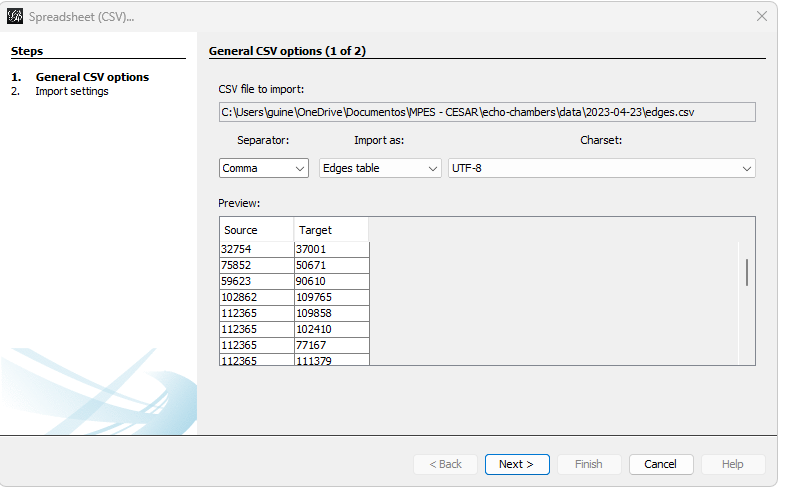
\includegraphics[scale=0.6]{images/gephi-edge-import.png}
\end{figure}

\subsection*{Carregando o conjunto de dados Colab no Gephi}
Após baixar o arquivo pré-processado descrito em \autoref{sec:preprocessing}, criamos um novo Workspace no Gephi e carregamos os arquivos de dados separadamente, começando pelo edges.csv. O arquivo nodes.csv é então carregado e o Gephi detecta automaticamente os carimbos de data e hora. Após importar ambos os arquivos, a tabela de dados do Gephi exibe os nós, as arestas e os carimbos de data e hora. A importação detectou 33818 nós e 66875 arestas. No entanto, devido ao alto número de conexões, a visualização do gráfico do Gephi exibe apenas um quadrado preto. Para corrigir isso e obter informações iniciais do conjunto de dados, precisamos escolher um Layout apropriado usando a guia de layout do Gephi.

\begin{figure}[!htb]
	\caption{Modelo de dados carregado no Gephi}
	\label{fig:gephi_data_table}
	\centering
	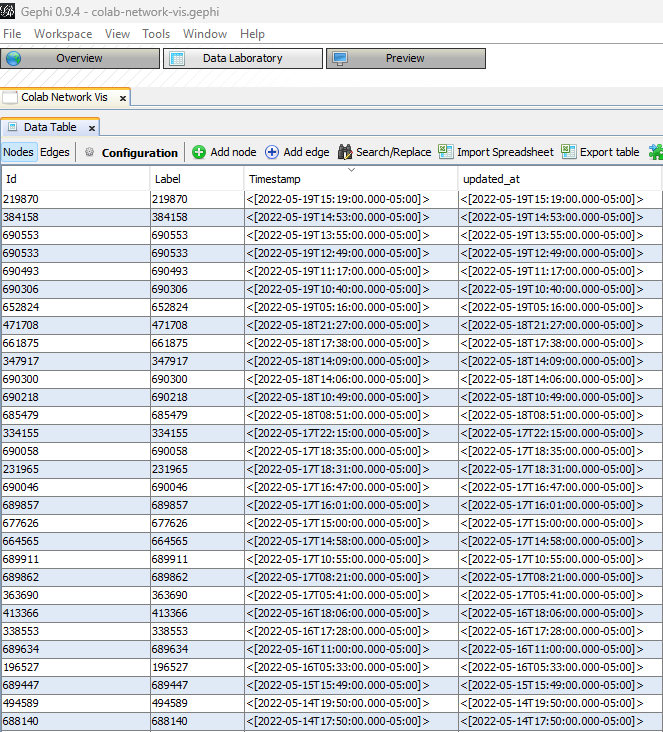
\includegraphics[scale=0.8]{images/gephi-data-table.png}
\end{figure}

\subsection*{Compreendendo os Layouts do Gephi}

Os layouts são um aspecto essencial da funcionalidade do Gephi, pois eles fornecem uma representação gráfica da estrutura da rede. O Gephi oferece vários presets de layout para gerar visualizações dos dados da rede em diversas formas. Cada preset utiliza um conjunto único de algoritmos para posicionar os nós e arestas da rede de maneira visualmente atraente. Nesta seção, examinaremos alguns dos layouts mais comuns do Gephi, seus casos de uso e sugeriremos o melhor layout para uma rede com tantas conexões.

Um dos layouts mais utilizados no Gephi é o layout Force Atlas. O layout Force Atlas é um layout baseado em forças que simula a física de um sistema massa-mola para organizar os nós da rede. Esse layout é particularmente útil para visualizar redes sociais, pois pode destacar aglomerados e comunidades de nós. O layout Force Atlas é especialmente adequado para redes de tamanho pequeno a médio, pois pode se tornar computacionalmente caro para redes maiores.

O layout Fruchterman-Reingold é outro layout popular no Gephi. Também é um layout baseado em forças que equilibra as forças de atração e repulsão entre os nós. Esse layout é particularmente útil para visualizar redes de tamanho pequeno a médio e pode ser usado para destacar aglomerados e comunidades de nós.

O layout Yifan Hu é um algoritmo baseado em forças desenvolvido por Yifan Hu em 2005. O algoritmo utiliza uma abordagem multinível para otimizar o layout dos nós em uma rede, minimizando uma função de energia que equilibra as forças de repulsão e atração entre os nós. Em cada nível, o algoritmo constrói uma representação mais grosseira da rede e a utiliza para guiar o layout da rede em níveis mais finos. Essa abordagem permite que o algoritmo lide com redes grandes e complexas, reduzindo a complexidade computacional do processo de layout. O layout Yifan Hu foi integrado em várias ferramentas de visualização de redes, incluindo o Gephi, como uma opção de layout padrão. A eficácia do layout foi demonstrada em diversos estudos, incluindo um estudo realizado por Lin (2019), que utilizaram o layout para visualizar a rede de coautoria de uma disciplina científica. Os resultados mostraram que o layout Yifan Hu foi capaz de visualizar efetivamente a estrutura da comunidade e destacar autores e publicações importantes dentro da rede.

Para uma rede com 66875 arestas, optamos por usar o layout Yifan Hu devido à sua capacidade de lidar com redes de grande escala, tornando-o adequado para o tamanho da rede fornecido. Além disso, o layout Yifan Hu é baseado em forças e pode otimizar o layout dos nós para fornecer uma representação visualmente agradável da rede. Posteriormente no experimento, pretendemos utilizar outros modelos de layout para obter diferentes insights do modelo de dados.

\subsection*{Visualizações do Gephi da Rede Colab}

O layout Yifan Hu foi aplicado ao conjunto de dados do Colab, resultando nesta imagem que apresenta dois clusters bem populados, uma quantidade considerável de nós de usuário e um grande número de nós isolados.

\begin{figure}[!hbtp]
	\caption{Rede do Colab renderizada com Layout Yifan Hu}
	\label{fig:colab_yifan_hu_first_set}
	\centering
	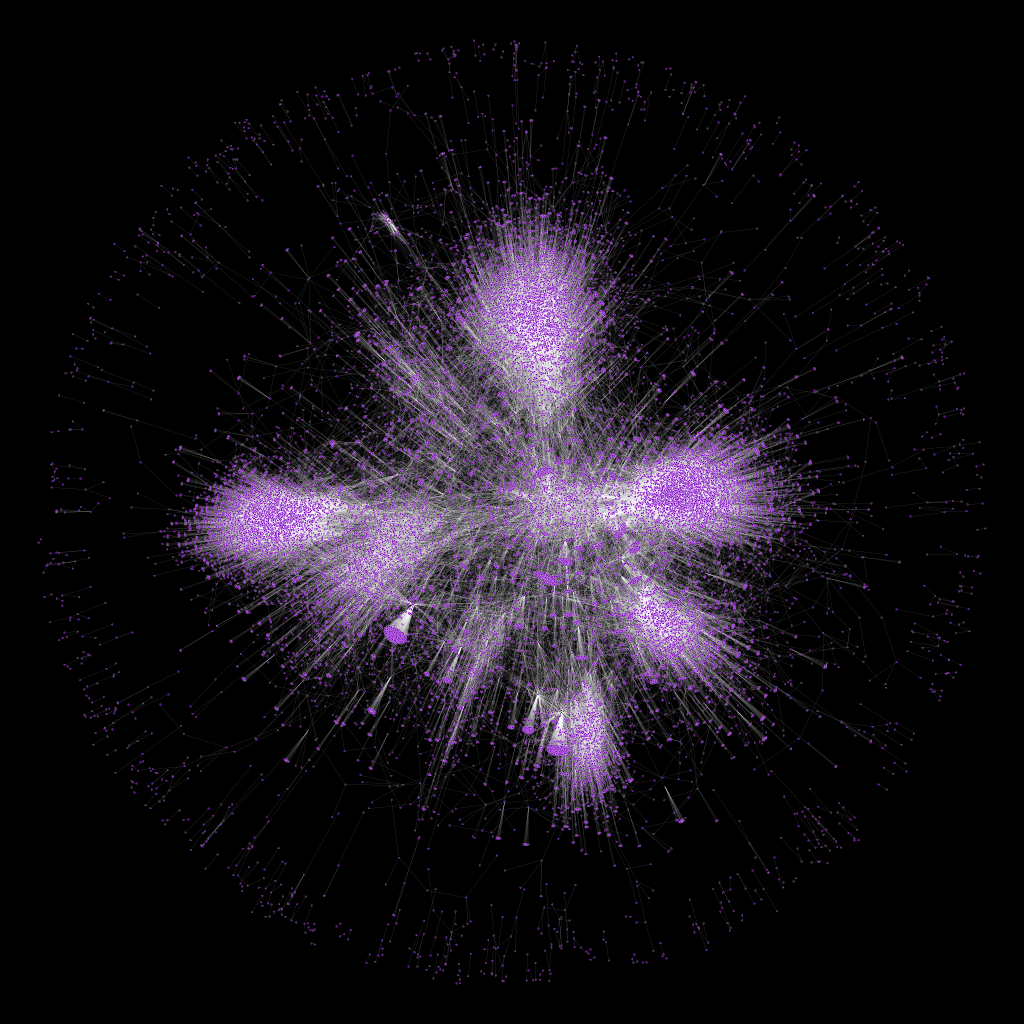
\includegraphics[scale=0.2]{images/colab-yifan-hu-first-set.png}
\end{figure}

O Yifan Hu nos proporciona um bom ponto de partida e algumas ideias iniciais. No entanto, para obter mais informações sobre o conjunto de dados, precisamos executar algumas estatísticas no Gephi e atualizar a aparência da visualização com os resultados das estatísticas. Vamos começar introduzindo as várias estatísticas do Gephi e avaliar como nossa análise de câmara de eco pode se beneficiar melhor de cada uma delas.

\subsection*{Explorando a Estrutura da Rede com as Estatísticas do Gephi}

\begin{figure}[!htb]
	\caption{Rede do Colab renderizada com Layout Yifan Hu e aparência dos nós enfatizando Centralidade.}
	\label{fig:colab_apperance_centrality}
	\centering
	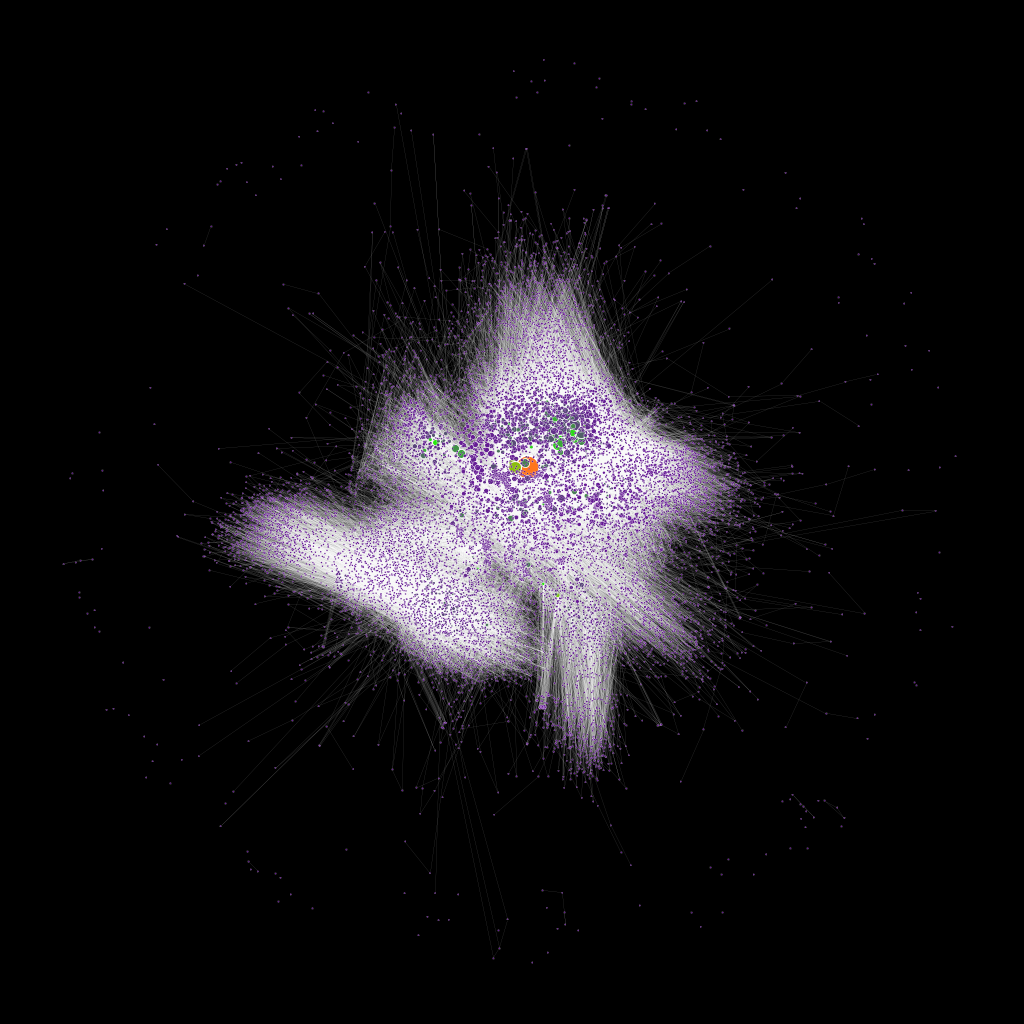
\includegraphics[scale=0.1]{images/colab-apperance-centrality.png}
	\fautor
\end{figure}

O Gephi oferece uma variedade de estatísticas que podem ajudar os pesquisadores a analisar e visualizar a estrutura das redes. Algumas das estatísticas mais comumente usadas na análise de redes sociais incluem grau, centralidade de intermediação (betweenness centrality) e coeficiente de agrupamento (clustering coefficient). O grau mede o número de conexões que um nó possui, enquanto a centralidade de intermediação identifica nós que desempenham um papel importante como pontes entre diferentes partes da rede. O coeficiente de agrupamento mede o grau em que os nós tendem a se agrupar em grupos.

Ao trabalhar com uma rede grande como o conjunto de dados do Colab, as estatísticas do Gephi podem ser particularmente úteis para obter insights sobre a estrutura subjacente da rede. Por exemplo, o grau pode ajudar a identificar nós com um grande número de conexões, enquanto a centralidade de intermediação pode destacar nós que são especialmente importantes para manter a conectividade geral da rede. O coeficiente de agrupamento pode ajudar a identificar grupos de nós que tendem a se agrupar, fornecendo informações sobre potenciais câmaras de eco ou outros padrões de agrupamento dentro da rede.

Algumas das estatísticas do Gephi mais úteis a serem consideradas incluem modularidade, detecção de comunidades e centralidade do Eigenvector. A modularidade mede o grau em que os nós dentro da rede se agrupam em grupos coesos, enquanto algoritmos de detecção de comunidades podem ajudar a identificar esses grupos com base em padrões de conectividade. A centralidade do Eigenvector, por outro lado, mede o grau em que um nó está conectado a outros nós altamente conectados dentro da rede.

Em nossa análise exploratória do conjunto de dados do Colab, começamos calculando o Diâmetro da Rede. A estatística de Diâmetro da Rede do Gephi mede a distância geodésica mais longa entre quaisquer dois nós na rede. Essa estatística é uma medida importante da conectividade da rede, pois reflete o grau em que os nós estão conectados entre si. Um diâmetro de rede baixo indica que os nós na rede estão intimamente conectados, enquanto um diâmetro de rede alto indica que os nós estão mais distantes uns dos outros. Essa estatística pode ser usada para identificar nós que são especialmente importantes para manter a conectividade da rede, bem como para detectar áreas da rede que podem estar mal conectadas.

A análise levou aproximadamente 10 minutos para ser concluída, o Diâmetro da Rede de 24 pode significar que a distância máxima entre quaisquer dois nós na rede é 24, indicando que a rede é relativamente compacta e bem conectada levando em conta o número total de nós. O Comprimento médio do caminho de 5.6 indica que, em média, são necessários pouco mais de cinco passos e meio para ir de um nó a outro na rede. Isso sugere que a rede possui caminhos relativamente curtos entre os nós, facilitando o fluxo de informações e influência pela rede. No geral, esses resultados sugerem que a rede está bem conectada, com um alto grau de interconectividade entre os nós.

Os resultados do Diâmetro da Rede e do comprimento médio do caminho sozinhos não são suficientes para determinar se a rede possui câmaras de eco. O diâmetro da rede e o comprimento médio do caminho fornecem informações sobre a estrutura geral da rede e como a informação pode se espalhar por ela. No entanto, para identificar câmaras de eco, precisamos examinar o coeficiente de agrupamento, a modularidade ou outras estatísticas de detecção de comunidades. Câmaras de eco geralmente têm níveis altos de agrupamento e uma pontuação baixa de modularidade, indicando grupos coesos que estão mais conectados entre si do que com o restante da rede. Ainda assim, podemos usar as configurações de aparência do Gephi para obter alguns insights adicionais. Depois de executar o algoritmo de diâmetro da rede, podemos usar suas métricas resultantes para alterar a aparência da nossa visualização da rede.

Especificamente, os nós foram coloridos de acordo com sua classificação de Centralidade de Proximidade (Closeness Centrality) e dimensionados de acordo com sua classificação de Centralidade de Intermediação (Betweenness Centrality). Essa abordagem permitiu uma representação clara dos nós que possuem alta centralidade em termos de sua importância na rede. Os nós com alta Centralidade de Proximidade foram coloridos em tons mais escuros de roxo, enquanto os nós com alta Centralidade de Intermediação foram dimensionados em tamanho maior. Essa combinação de atributos dos nós destacou efetivamente os nós mais importantes em termos de sua conectividade e posição na rede. Isso pode ajudar a identificar nós que são mais centrais para a rede, pois serão coloridos em tons mais escuros. Além disso, pode ajudar a identificar nós que estão mais isolados do restante da rede, pois serão coloridos em tons de laranja.

\subsection*{Otimizando visualizações com Filtragem no Gephi}

Em ambas as imagens, é perceptível uma prevalência de nós isolados. Após uma análise mais aprofundada, descobrimos que a maioria dos nós isolados são de fato de usuários sem seguidores no arquivo de conexões. Alguns deles são de usuários que seguiram outro usuário em algum momento, mas deixaram de seguir dentro do período em que o conjunto de dados foi capturado. Para mitigar a quantidade de nós isolados, utilizamos a filtragem do Gephi, pois ela pode ser aplicada apenas na visualização, preservando o conjunto de dados. A filtragem é uma etapa essencial na análise de redes, pois permite que os pesquisadores foquem em aspectos específicos da rede e removam informações irrelevantes ou ruidosas. No contexto da detecção de câmaras de eco, a filtragem é especialmente crucial, pois ajuda a identificar comunidades relevantes e reduz o impacto de nós isolados que podem não ser representativos da estrutura geral da rede. A filtragem é uma etapa crucial na análise de redes e tem sido amplamente estudada na literatura.
\citeonline{2016_Fortunato} destacaram a importância da filtragem na detecção de comunidades, pois ela pode impactar significativamente a qualidade e a precisão dos resultados. Da mesma forma, \citeonline{2010_Newman_BOOK} discutiu os desafios de lidar com dados ruidosos na análise de redes e sugeriu várias técnicas de filtragem para melhorar a qualidade da análise. Em particular, a filtragem com base no grau tem sido amplamente utilizada na análise de redes, pois permite que os pesquisadores foquem nos nós e comunidades mais importantes da rede \cite[]{2002_Borgatti}.

Para filtrar nós irrelevantes ou isolados, aplicamos várias etapas de filtragem no laboratório de dados do Gephi. Começamos removendo laços e arestas múltiplas, que podem criar informações redundantes e complicar a análise. Em seguida, removemos nós com baixo grau, ou seja, aqueles que possuíam poucas conexões com outros nós na rede. Optamos por usar um filtro de Grau a partir de 4 para destacar apenas comunidades compostas por pelo menos 4 usuários. Essa etapa nos permitiu focar em comunidades que tinham mais probabilidade de serem significativas em termos de fluxo de informações e interações de usuários. Também removemos nós que não estavam conectados a nenhum outro nó na rede.

\section{Topologia da Rede Colab}
Após aplicar as configurações de aparência, os agrupamentos de usuários se tornam mais visíveis, assim como a centralidade de alguns usuários-chave. No entanto, ainda existem outras estatísticas que podemos executar no Gephi para obter uma visão mais abrangente. A tabela abaixo apresenta um resumo de todas as métricas obtidas a partir das Estatísticas do Gephi:

\begin{table}[h]
	\centering
	\caption{Resumo das Estatísticas do Gephi}
	\label{tab:colab_gephi_statistics}
	\begin{tabular}{|l|l|l|}
		\hline
		\textbf{Relatório Gephi}    & \textbf{Chave}               & \textbf{Valor}     \\
		\hline
		Topologia                   & Nós                          & 33818              \\
		Topologia                   & Arestas                      & 66875              \\
		Diâmetro da Rede            & Comprimento Médio do Caminho & 5.623615966246081  \\
		Modularidade                & Modularidade                 & 0.683              \\
		Modularidade                & Número de Comunidades        & 352                \\
		Centralidade de Eigenvector & Mudança da Soma              & 0.3087450789952254 \\
		Centralidade de Eigenvector & Número de Iterações          & 100                \\
		Coeficiente de Agrupamento  & Média                        & 0.171              \\
		Componentes Conectados      & Fracamente Conectados        & 329                \\
		Componentes Conectados      & Fortemente Conectados        & 28119              \\
		PageRank                    & Epsilon                      & 0.001              \\
		PageRank                    & Probabilidade                & 0.85               \\
		Inferência Estatística      & Comprimento da Descrição     & 1184001.357        \\
		Inferência Estatística      & Número de Comunidades        & 1367               \\
		\hline
	\end{tabular}
\end{table}

Os resultados das estatísticas do Gephi executadas no conjunto de dados do Colab fornecem informações sobre a estrutura da rede e as potenciais câmaras de eco. O diâmetro da rede de 24 e o comprimento médio do caminho de 5,62 indicam que a rede é relativamente pequena e fortemente conectada. Isso sugere que as informações podem se espalhar rapidamente pela rede e que pode haver um alto grau de homofilia entre os nós, o que pode contribuir para a formação de câmaras de eco \cite[]{2012_Kadushin_BOOK}.

O valor de modularidade de 0,683 e o número de comunidades de 352 sugerem que a rede possui um grau relativamente alto de estrutura de comunidades, com muitos grupos distintos de nós que estão mais densamente conectados entre si do que a nós fora de sua comunidade. Isso é consistente com a ideia de câmaras de eco, já que grupos mais densamente conectados e insulares podem ser mais propensos a desenvolver e reforçar crenças e valores compartilhados \cite[]{2016_Vicario}.

Os valores de centralidade de eigenvector, com mudança total de 0,31 e número de iterações de 100, sugerem que existem alguns nós altamente influentes na rede que têm um impacto desproporcional na propagação de informações. Isso está de acordo com a ideia de "líderes de opinião" ou "influenciadores" em redes sociais
\cite[]{1955_Katz_BOOK}. Esses nós podem desempenhar um papel fundamental na formação e no reforço de câmaras de eco, já que suas crenças e valores podem ter mais probabilidade de se espalhar pela rede.

O coeficiente de clusterização médio de 0,171 sugere que existe um grau moderado de agrupamento na rede, ou seja, os nós tendem a se conectar a outros nós que já estão conectados a eles. Isso pode contribuir para a formação de câmaras de eco, já que nós que compartilham crenças ou valores têm mais probabilidade de se agrupar juntos \cite[]{1998_Watts}.

Os valores de componentes conectados, com 329 fracamente conectados e 28.119 fortemente conectados, sugerem que a rede possui um grande número de componentes fortemente conectados, ou seja, existem muitos grupos de nós que estão completamente ou quase completamente conectados entre si, mas não a outros nós na rede. Isso está de acordo com a ideia de câmaras de eco, já que grupos mais fortemente conectados e insulares podem ser mais propensos a desenvolver crenças e valores compartilhados \cite[]{2016_Vicario}.

Os valores de PageRank, com epsilon de 0,001 e probabilidade de 0,85, sugerem que existem alguns nós altamente influentes na rede que têm um impacto significativo na propagação de informações. Isso está em consonância com os resultados da centralidade de eigenvector e sugere que esses nós podem desempenhar um papel fundamental na formação e no reforço de câmaras de eco.

Os valores de inferência estatística, com comprimento da descrição de 1.184.001,36 e número de comunidades de 1.367, sugerem que existem muitas comunidades distintas na rede com diferentes padrões de conexões e interações. Isso está de acordo com as estratégias de fornecimento de conteúdo do aplicativo, pois essas comunidades podem ser locais por natureza. Além disso, é consistente com os resultados de modularidade e sugere que pode haver múltiplas câmaras de eco dentro da rede com diferentes crenças e valores, embora não possamos afirmar isso com certeza sem levar em conta o aspecto de localização.

No geral, as estatísticas do Gephi fornecem evidências de que a rede possui um alto grau de estrutura de comunidades, agrupamento e nós influentes, o que pode contribuir para a formação e o reforço de câmaras de eco. No entanto, mais pesquisas são necessárias para confirmar se as câmaras de eco estão presentes na rede e como estão estruturadas.

\subsection{Centralizade de Rede}

\begin{figure}[!hbtp]
	\caption{Rede do Colab renderizada com Layout OpenOrd}
	\label{fig:colab_openord}
	\centering
	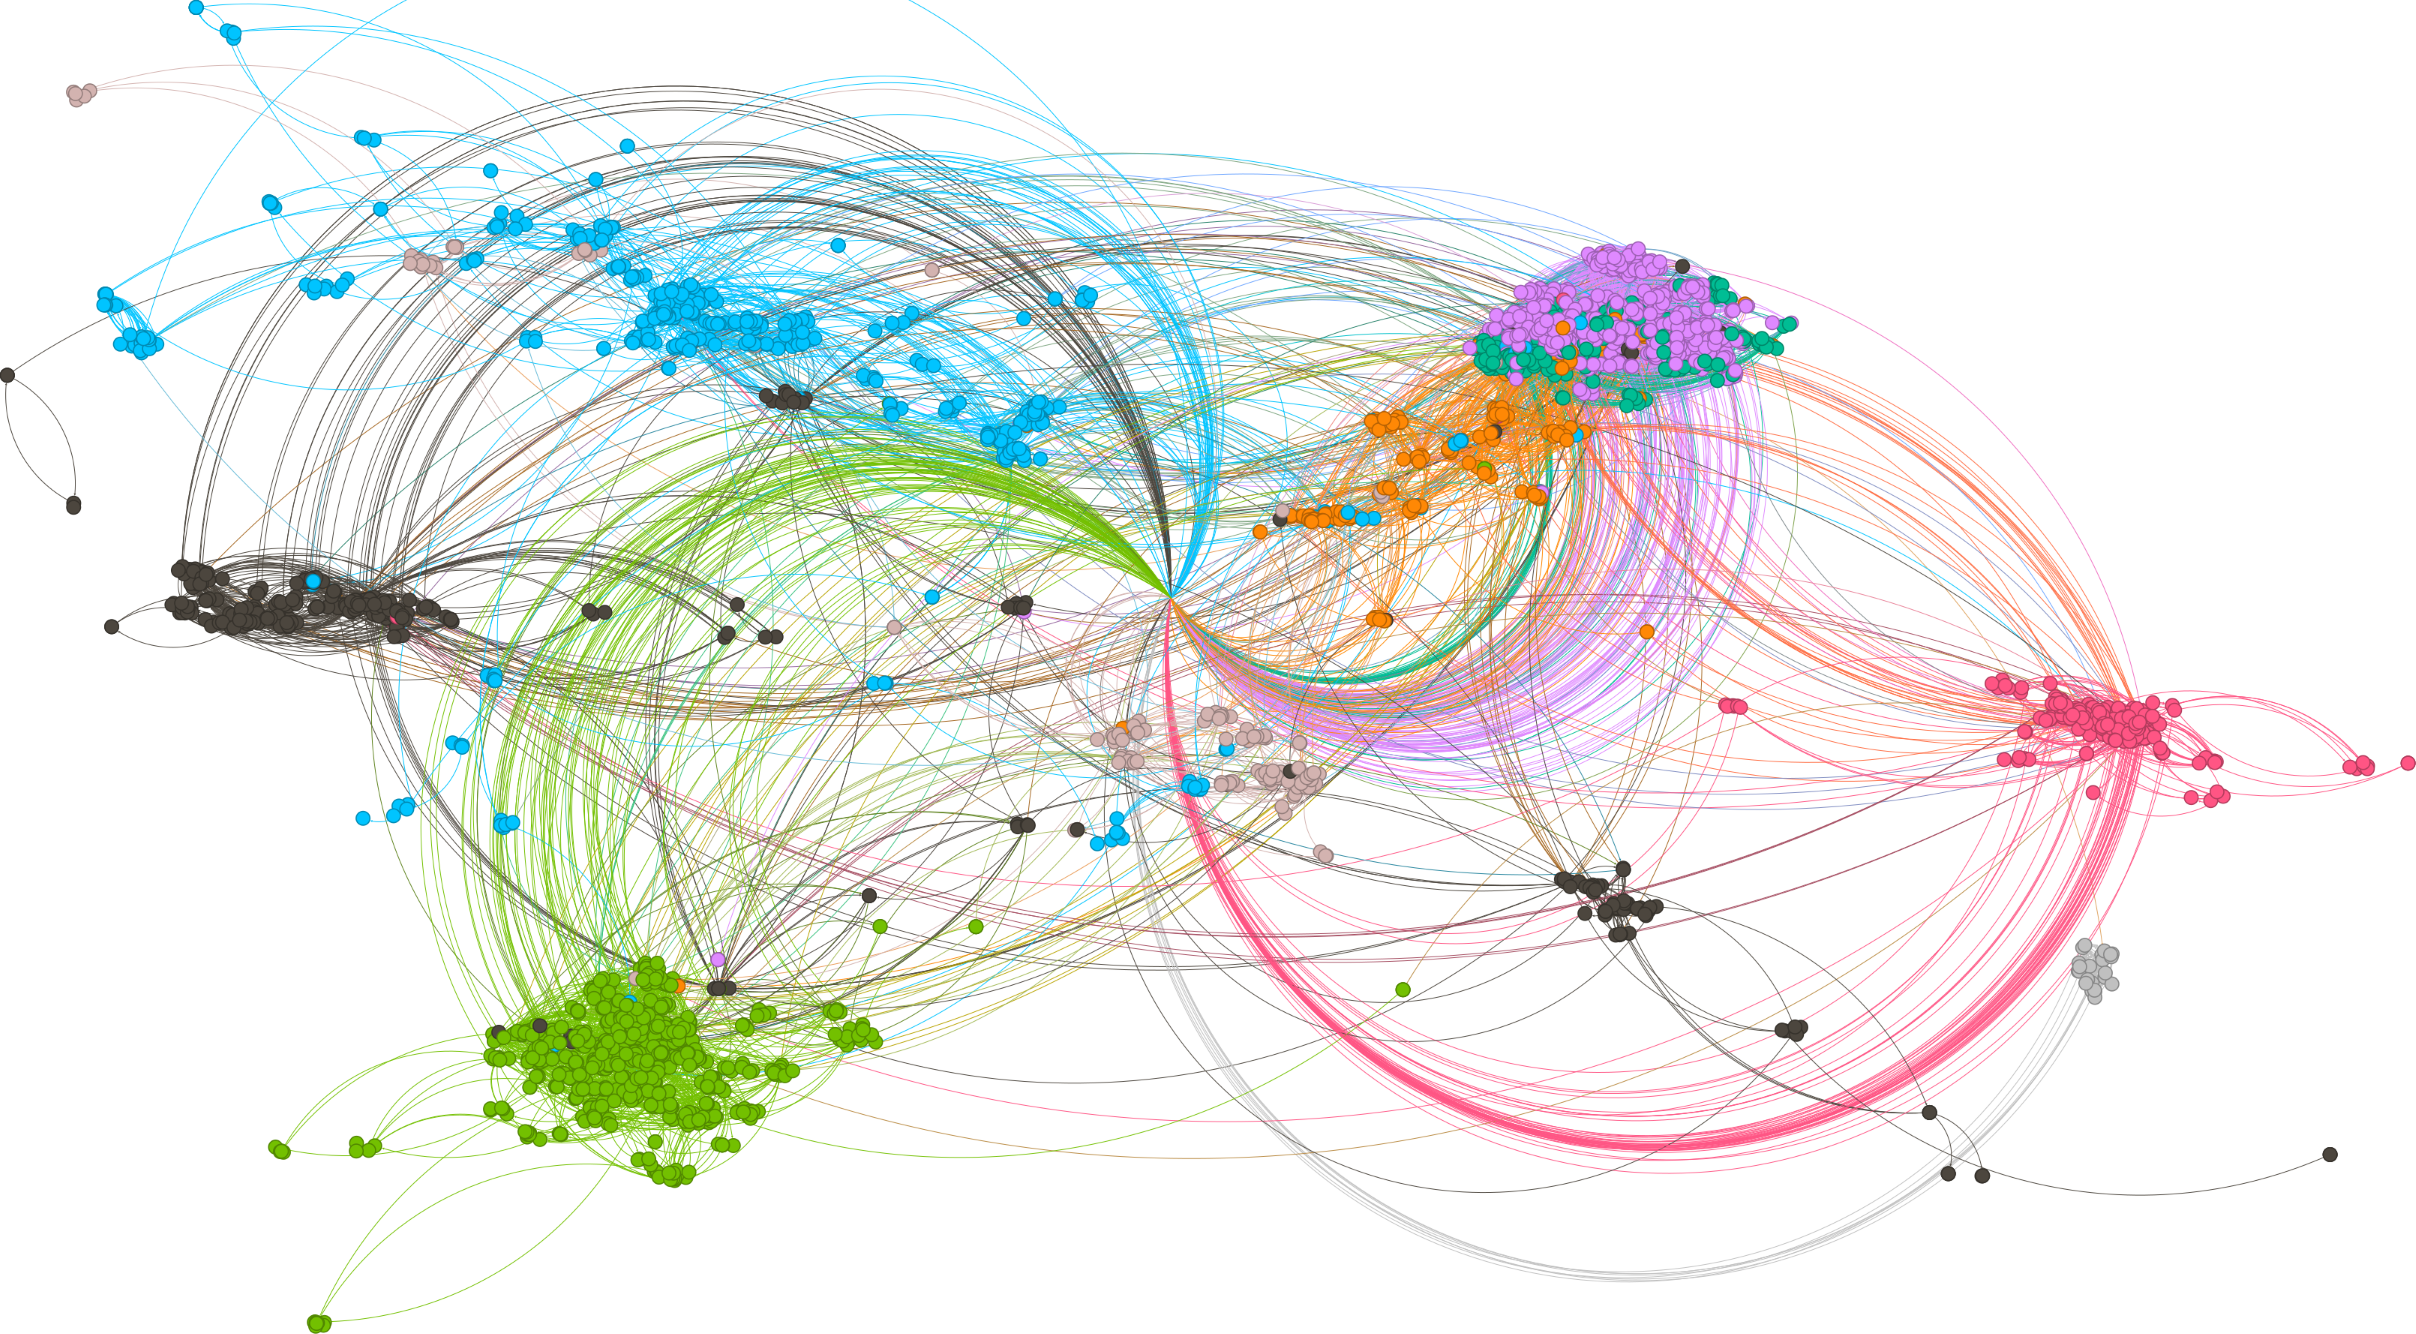
\includegraphics[scale=0.20]{images/colab-openord.png}
	\fautor
\end{figure}

Outra opção para visualizar centralidade é usar o algoritmo OpenOrd, um algoritmo de layout baseado em forças que é frequentemente usado em visualização e análise de redes. Uma das vantagens do algoritmo OpenOrd é sua capacidade de visualizar efetivamente a centralidade de intermediação em redes grandes e complexas. A centralidade de intermediação é uma medida da importância de um nó em uma rede, com base em sua capacidade de atuar como uma "ponte" ou "hub" entre diferentes partes da rede. Ao visualizar a centralidade de intermediação com o algoritmo OpenOrd, podemos identificar nós que desempenham um papel crucial na conexão de diferentes comunidades ou grupos dentro de uma rede.

Por exemplo, em um estudo sobre a comunicação no Twitter durante uma crise política, o algoritmo OpenOrd foi usado para visualizar a centralidade de intermediação de diferentes usuários do Twitter. Os resultados revelaram vários usuários com alta centralidade de intermediação, sugerindo que esses usuários desempenharam um papel fundamental na conexão de diferentes grupos de usuários do Twitter e na disseminação de informações durante a crise \cite[text]{2011_Poblete_IP}.

\begin{figure}[!hbtp]
	\caption{Rede do Colab destacando centralidade}
	\label{fig:colab_centrality}
	\centering
	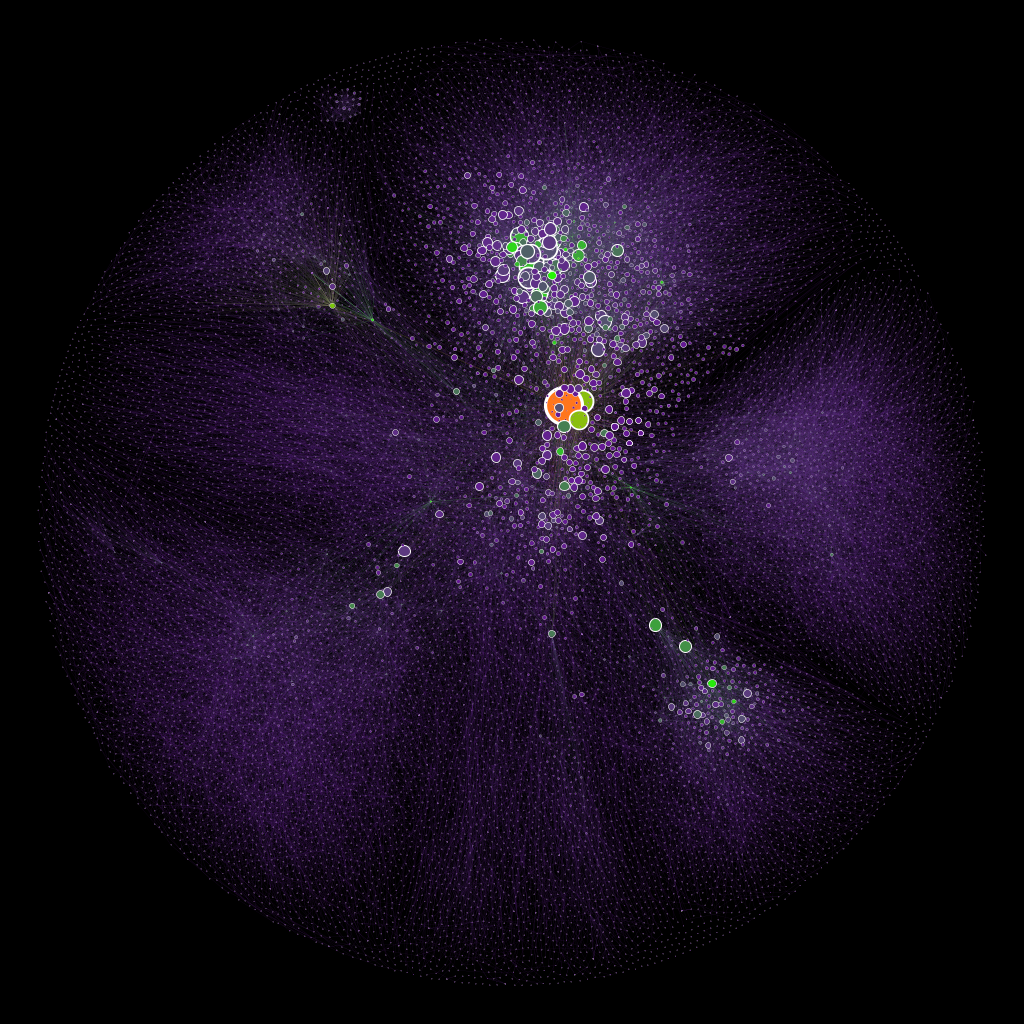
\includegraphics[scale=0.15]{images/colab-centrality.png}
	\fautor
\end{figure}

A visualização da rede Colab usando o algoritmo OpenOrd mostra uma clara distinção entre os nós com base em suas medidas de centralidade. Os nós maiores com maior centralidade de Eigenvector são mais influentes na rede e podem ter um impacto maior no fluxo de informações. O nó laranja, com a maior pontuação de centralidade de Eigenvector de 1.0, se destaca como o nó mais influente. No entanto, é interessante observar que esse nó tem uma pontuação de centralidade de intermediação relativamente baixa de 0.014, indicando que ele pode não servir necessariamente como um conector crítico entre diferentes partes da rede. Por outro lado, o nó verde no topo possui a segunda maior pontuação de centralidade de Eigenvector de 0.599 e pode atuar como um conector mais importante, com uma pontuação de centralidade de intermediação mais alta. No geral, os resultados sugerem que a rede é dominada por alguns nós altamente conectados, que podem ter um impacto significativo na estrutura e função geral da rede.

A centralidade desses usuários traz à tona o uso de cliques no contexto da Análise de Redes Sociais. Cliques podem ser um fator importante na identificação de câmaras de eco em redes. Um clique é um grupo de nós que estão todos conectados entre si, formando um subgrafo completo. Ao identificar cliques em uma rede, podemos começar a entender a estrutura da câmara de eco e como ela está conectada à rede mais ampla.

Para visualizar cliques no Gephi, uma abordagem é usar a estatística interna "Coeficiente de Agrupamento" para identificar nós que pertencem a aglomerados altamente conectados, que podem representar cliques. Após calcular o coeficiente de agrupamento para cada nó, é possível filtrar a rede para mostrar apenas nós com um coeficiente alto, como aqueles acima de um determinado limite. Em seguida, ajustando o tamanho e a cor dos nós na guia Aparência para refletir o número de conexões ou alguma outra métrica de interesse, os cliques podem ser visualizados como aglomerados densamente conectados de nós de cores e tamanhos semelhantes. Além disso, o uso dos algoritmos de agrupamento incorporados do Gephi, como o método Louvain ou otimização de modularidade, também pode ajudar a identificar e visualizar cliques em uma rede.

\begin{figure}[!hbtp]
	\centering
	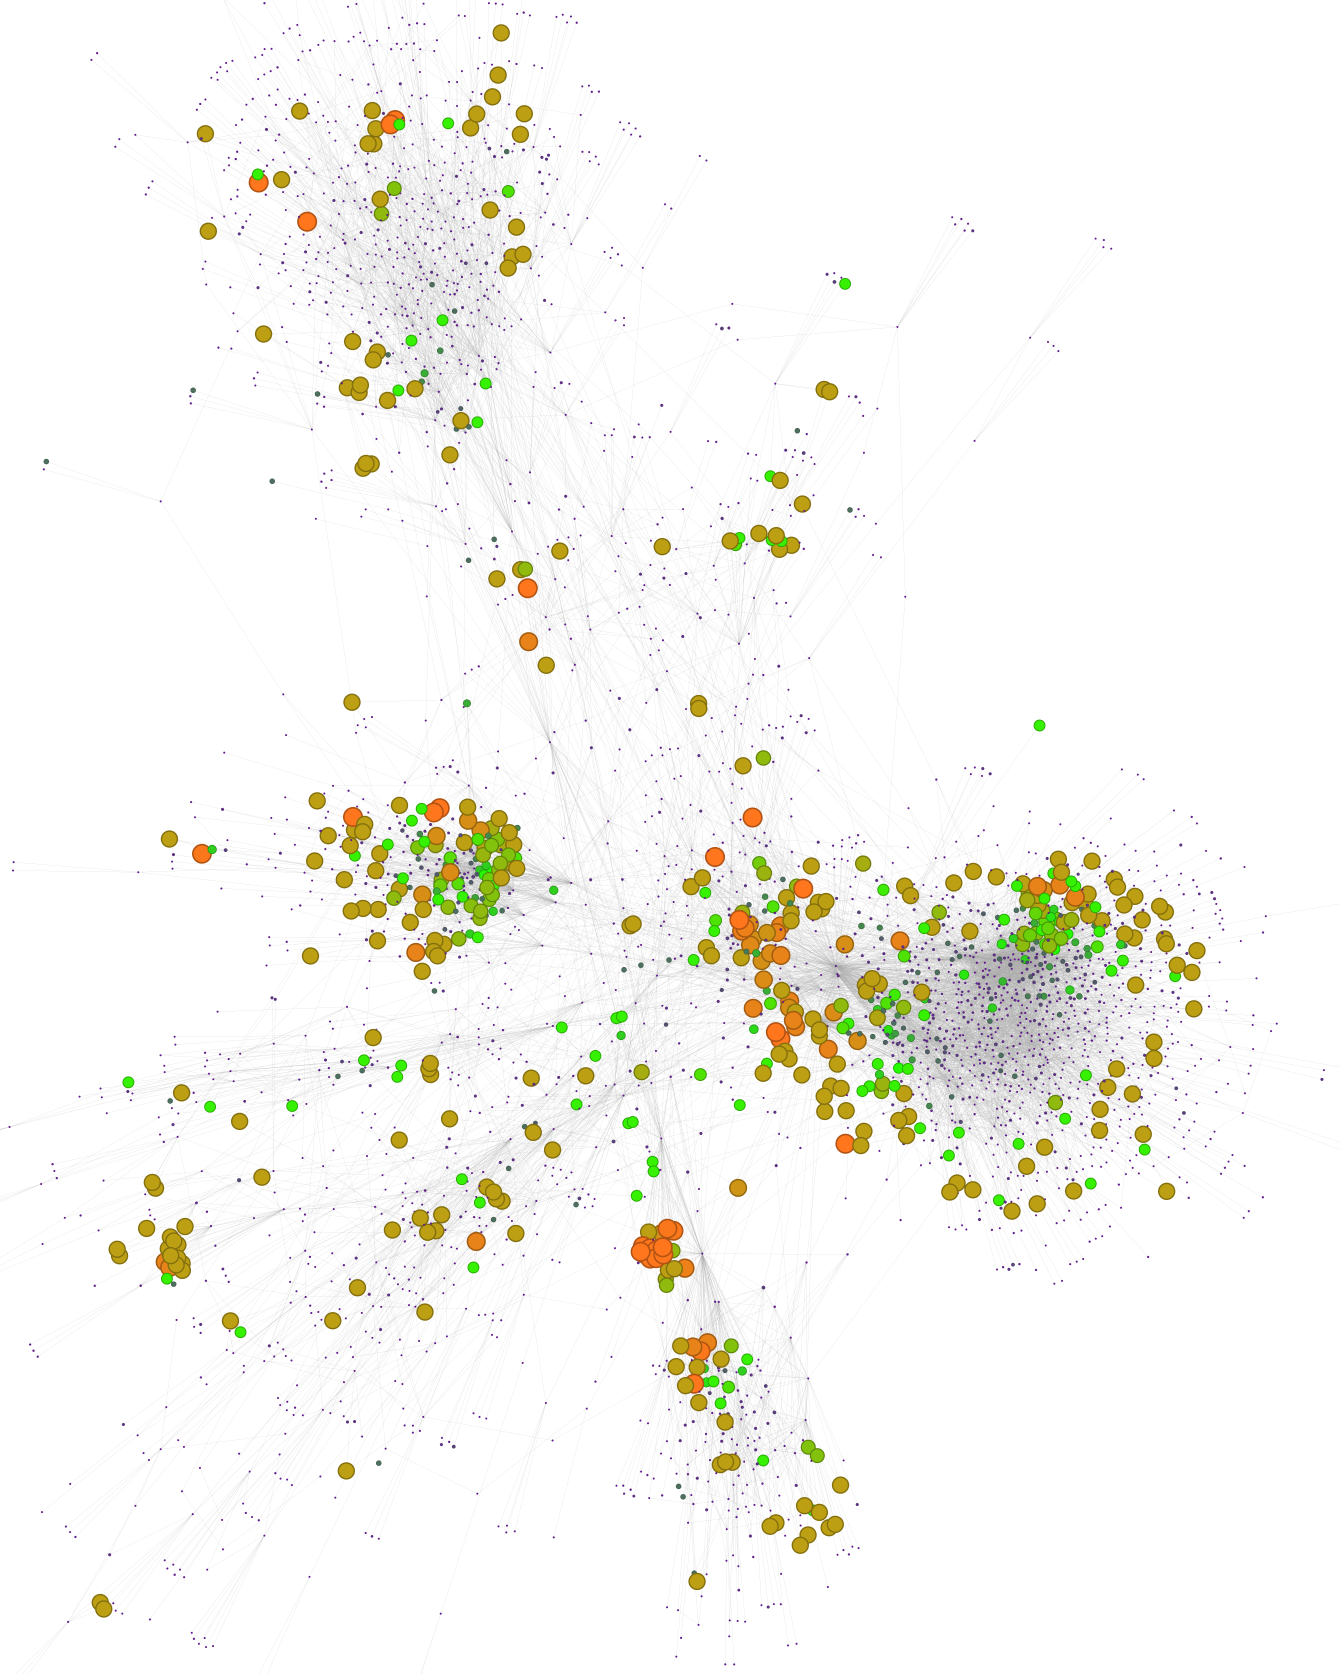
\includegraphics[scale=0.45]{images/colab-cliques.png}
	\caption{Visualização dos cliques identificados na rede. Nós que fazem parte de cliques são destacados em laranja, indicando subcomunidades altamente interconectadas. Nós verdes fazem parte de subcomunidades menores que orbitam os cliques. Nós roxos não fazem parte de nenhum clique.}
	\label{fig:gephi_cliques}
	\fautor
\end{figure}

Os cliques, sendo subgrafos completos, representam grupos de nós que estão altamente conectados entre si. Essa coesividade pode indicar subcomunidades fortemente interconectadas ou grupos de indivíduos com interações muito frequentes. A identificação desses cliques pode fornecer insights valiosos sobre a estrutura e dinâmica da rede, especialmente em contextos onde a formação de subgrupos coesos é de interesse, como em redes sociais ou colaborativas.

No entanto, apenas os cliques podem não ser suficientes para identificar câmaras de eco, pois podem estar em jogo outros fatores, como homofilia ou viés de confirmação. Portanto, é importante usar múltiplas abordagens e métricas, como detecção de comunidades e análise de conteúdo, para obter uma compreensão mais abrangente das câmaras de eco na rede.

Enquanto os cliques nos oferecem uma visão sobre subgrupos coesos dentro da rede, é essencial também considerar a influência individual de cada nó para compreender a dinâmica da rede como um todo. Nesse contexto, a centralidade de eigenvector emerge como uma métrica valiosa. Proposta por \citeonline{1972_Bonacich}, essa métrica não se limita a contar as conexões diretas de um nó, mas pondera essas conexões com base na influência dos nós a que estão conectadas. Assim, um nó conectado a outros nós influentes terá uma pontuação de centralidade de eigenvector mais alta. Esta métrica é particularmente útil para identificar atores-chave em redes sociais, pois destaca aqueles que, mesmo que não estejam diretamente conectados a muitos outros, estão estrategicamente posicionados na rede. Em nossa análise, a centralidade de eigenvector nos ajudará a identificar os usuários mais influentes no Colab, complementando nossa compreensão obtida através da identificação de cliques.

\begin{figure}[!hbtp]
	\caption{Visualização destacando os usuários mais influentes na rede}
	\label{fig:colab_users_graph}
	\centering
	\includegraphics[scale=0.28]{images/colab-users-graph.png}
	\fautor
\end{figure}

Na Figura \ref{fig:colab_users_graph}, a estatística de modularidade do Gephi foi empregada para discernir e colorir distintas comunidades na rede do Colab. Ao analisar a distribuição das comunidades, observa-se que as dez primeiras comunidades representam uma proporção significativa da rede, indicando que uma parte considerável dos nós está concentrada nessas comunidades principais.

A centralidade de eigenvector revela insights interessantes sobre a influência dos nós dentro dessas comunidades. Uma proporção notável de nós tem uma pontuação de eigenvector de 0,0, sugerindo que muitos usuários, embora pertencentes a comunidades, podem não ter uma influência direta significativa. No entanto, a presença de nós com pontuações de centralidade de eigenvector consideravelmente altas, até mesmo superiores a 1, destaca a existência de usuários-chave que atuam como hubs centrais em suas respectivas comunidades.

Estes hubs, com alta centralidade de eigenvector, desempenham um papel crucial na disseminação de informações e na formação de opiniões dentro de suas comunidades. Em algumas comunidades, observa-se mais de um hub, indicando uma estrutura de rede mais complexa com múltiplos canais de influência. Esta configuração sugere que, enquanto algumas comunidades podem ter um único ponto focal dominante, outras podem ter uma distribuição de influência mais equilibrada entre vários membros-chave.

A análise reforça a ideia de homofilia, onde usuários com opiniões ou características semelhantes tendem a se agrupar. A interação entre a estrutura das comunidades e a distribuição da centralidade de eigenvector sugere uma rede onde determinados usuários desempenham papéis cruciais, não apenas em termos de número de conexões, mas também em termos de influência qualitativa dentro de suas comunidades.

\subsection{Comunidades}

Visualizar um conjunto de dados do Gephi focando nas comunidades pode ser altamente benéfico para explorar a estrutura de redes complexas, como redes sociais, e identificar potenciais câmaras de eco. Ao identificar comunidades ou grupos dentro de uma rede, podemos obter insights sobre o comportamento de subgrupos dentro da rede maior e como eles podem interagir entre si. Uma abordagem popular para detectar comunidades em redes é o algoritmo de detecção de comunidades baseado em modularidade desenvolvido por \citeonline{2008_Blondel}. Esse algoritmo particiona os nós em comunidades, maximizando uma função de qualidade conhecida como modularidade, que mede a densidade de conexões dentro de uma comunidade em comparação com as conexões entre comunidades. Este método é frequentemente referido como o algoritmo "Louvain" em homenagem a instituição dos pesquisadores.

\subsection{Visualizando Comunidades no Gephi}

Ao configurar a aparência da visualização do Gephi, focamos em destacar as comunidades por meio de codificação de cores e tamanho. Especificamente, usamos a estatística de Modularidade para atribuir uma cor única a cada comunidade, facilitando a distinção visual entre diferentes subgrupos na rede. Além disso, aumentamos o tamanho dos nós dentro de cada comunidade para destacar sua importância dentro do subgrupo. Essas indicações visuais podem ajudar a identificar rapidamente potenciais câmaras de eco dentro da rede.

\begin{figure}[!hbtp]
	\caption{Rede do Colab destacando comunidades}
	\label{fig:colab_communities}
	\centering
	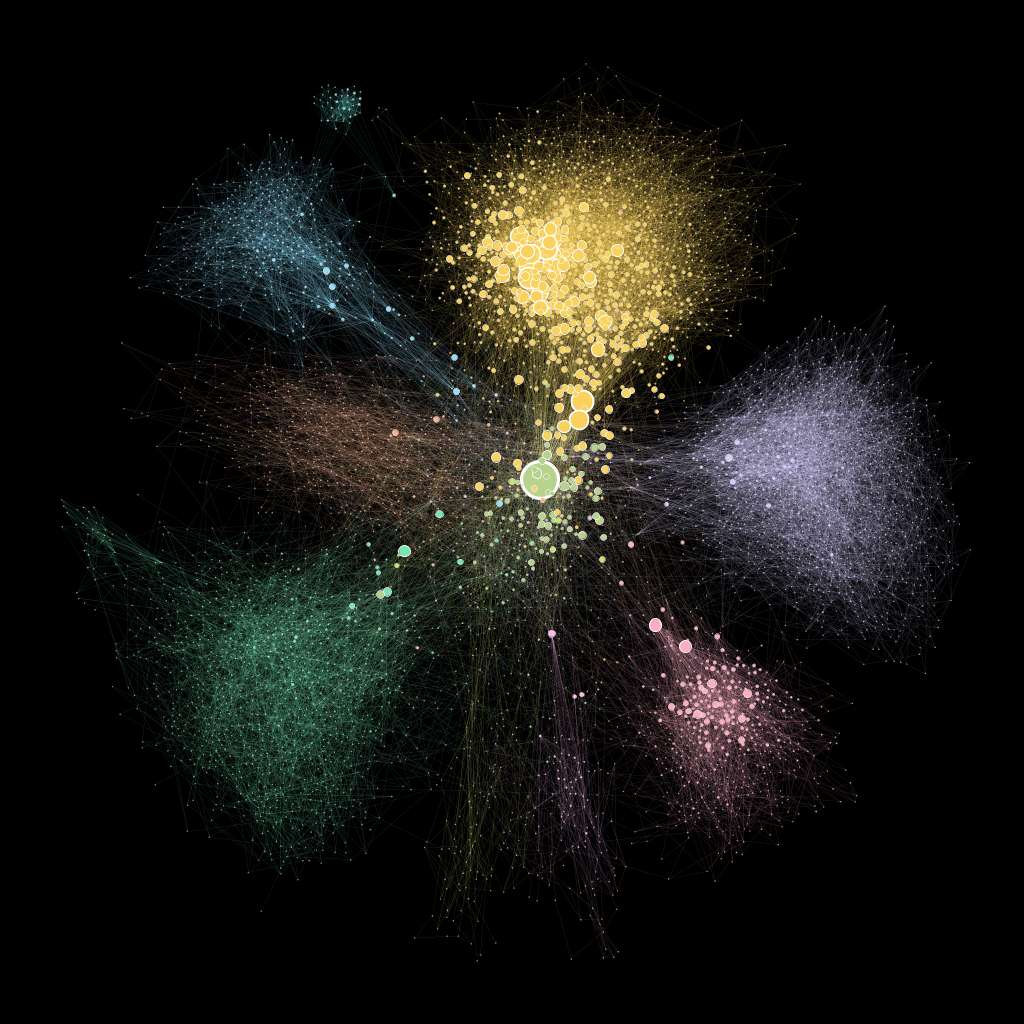
\includegraphics[scale=0.25]{images/colab-communities.png}
	\fautor
\end{figure}

Pesquisas mostram que visualizar comunidades dentro de uma rede pode ajudar a identificar câmaras de eco. Por exemplo, um estudo realizado por \citeonline{2018_Fortunato_IP} demonstrou que visualizar comunidades dentro de uma rede pode ajudar a detectar câmaras de eco e entender sua estrutura. Em nosso estudo, aplicamos abordagens semelhantes para detectar comunidades e visualizar nossa rede, o que nos permitiu identificar potenciais câmaras de eco e analisar ainda mais sua influência na disseminação de informações. O trabalho de \cite{2014_Colleoni} também 

Em resumo, visualizar um conjunto de dados do Gephi focando em comunidades pode fornecer insights valiosos sobre a estrutura de redes complexas e auxiliar na detecção de potenciais câmaras de eco. Ao usar codificação de cores e tamanho para destacar comunidades, podemos identificar rapidamente subgrupos dentro da rede e compreender melhor como eles interagem entre si. Essa abordagem é apoiada pelo trabalho de \citeonline{2010_Fortunato} e pode ser usada para obter insights sobre o comportamento de redes sociais e possíveis fontes de polarização.

\begin{figure}[!hbtp]
	\caption{Distribuição geográfica das comunidades da rede do Colab sobreposto ao mapa do Brasil}
	\label{fig:colab_geoclusters}
	\centering
	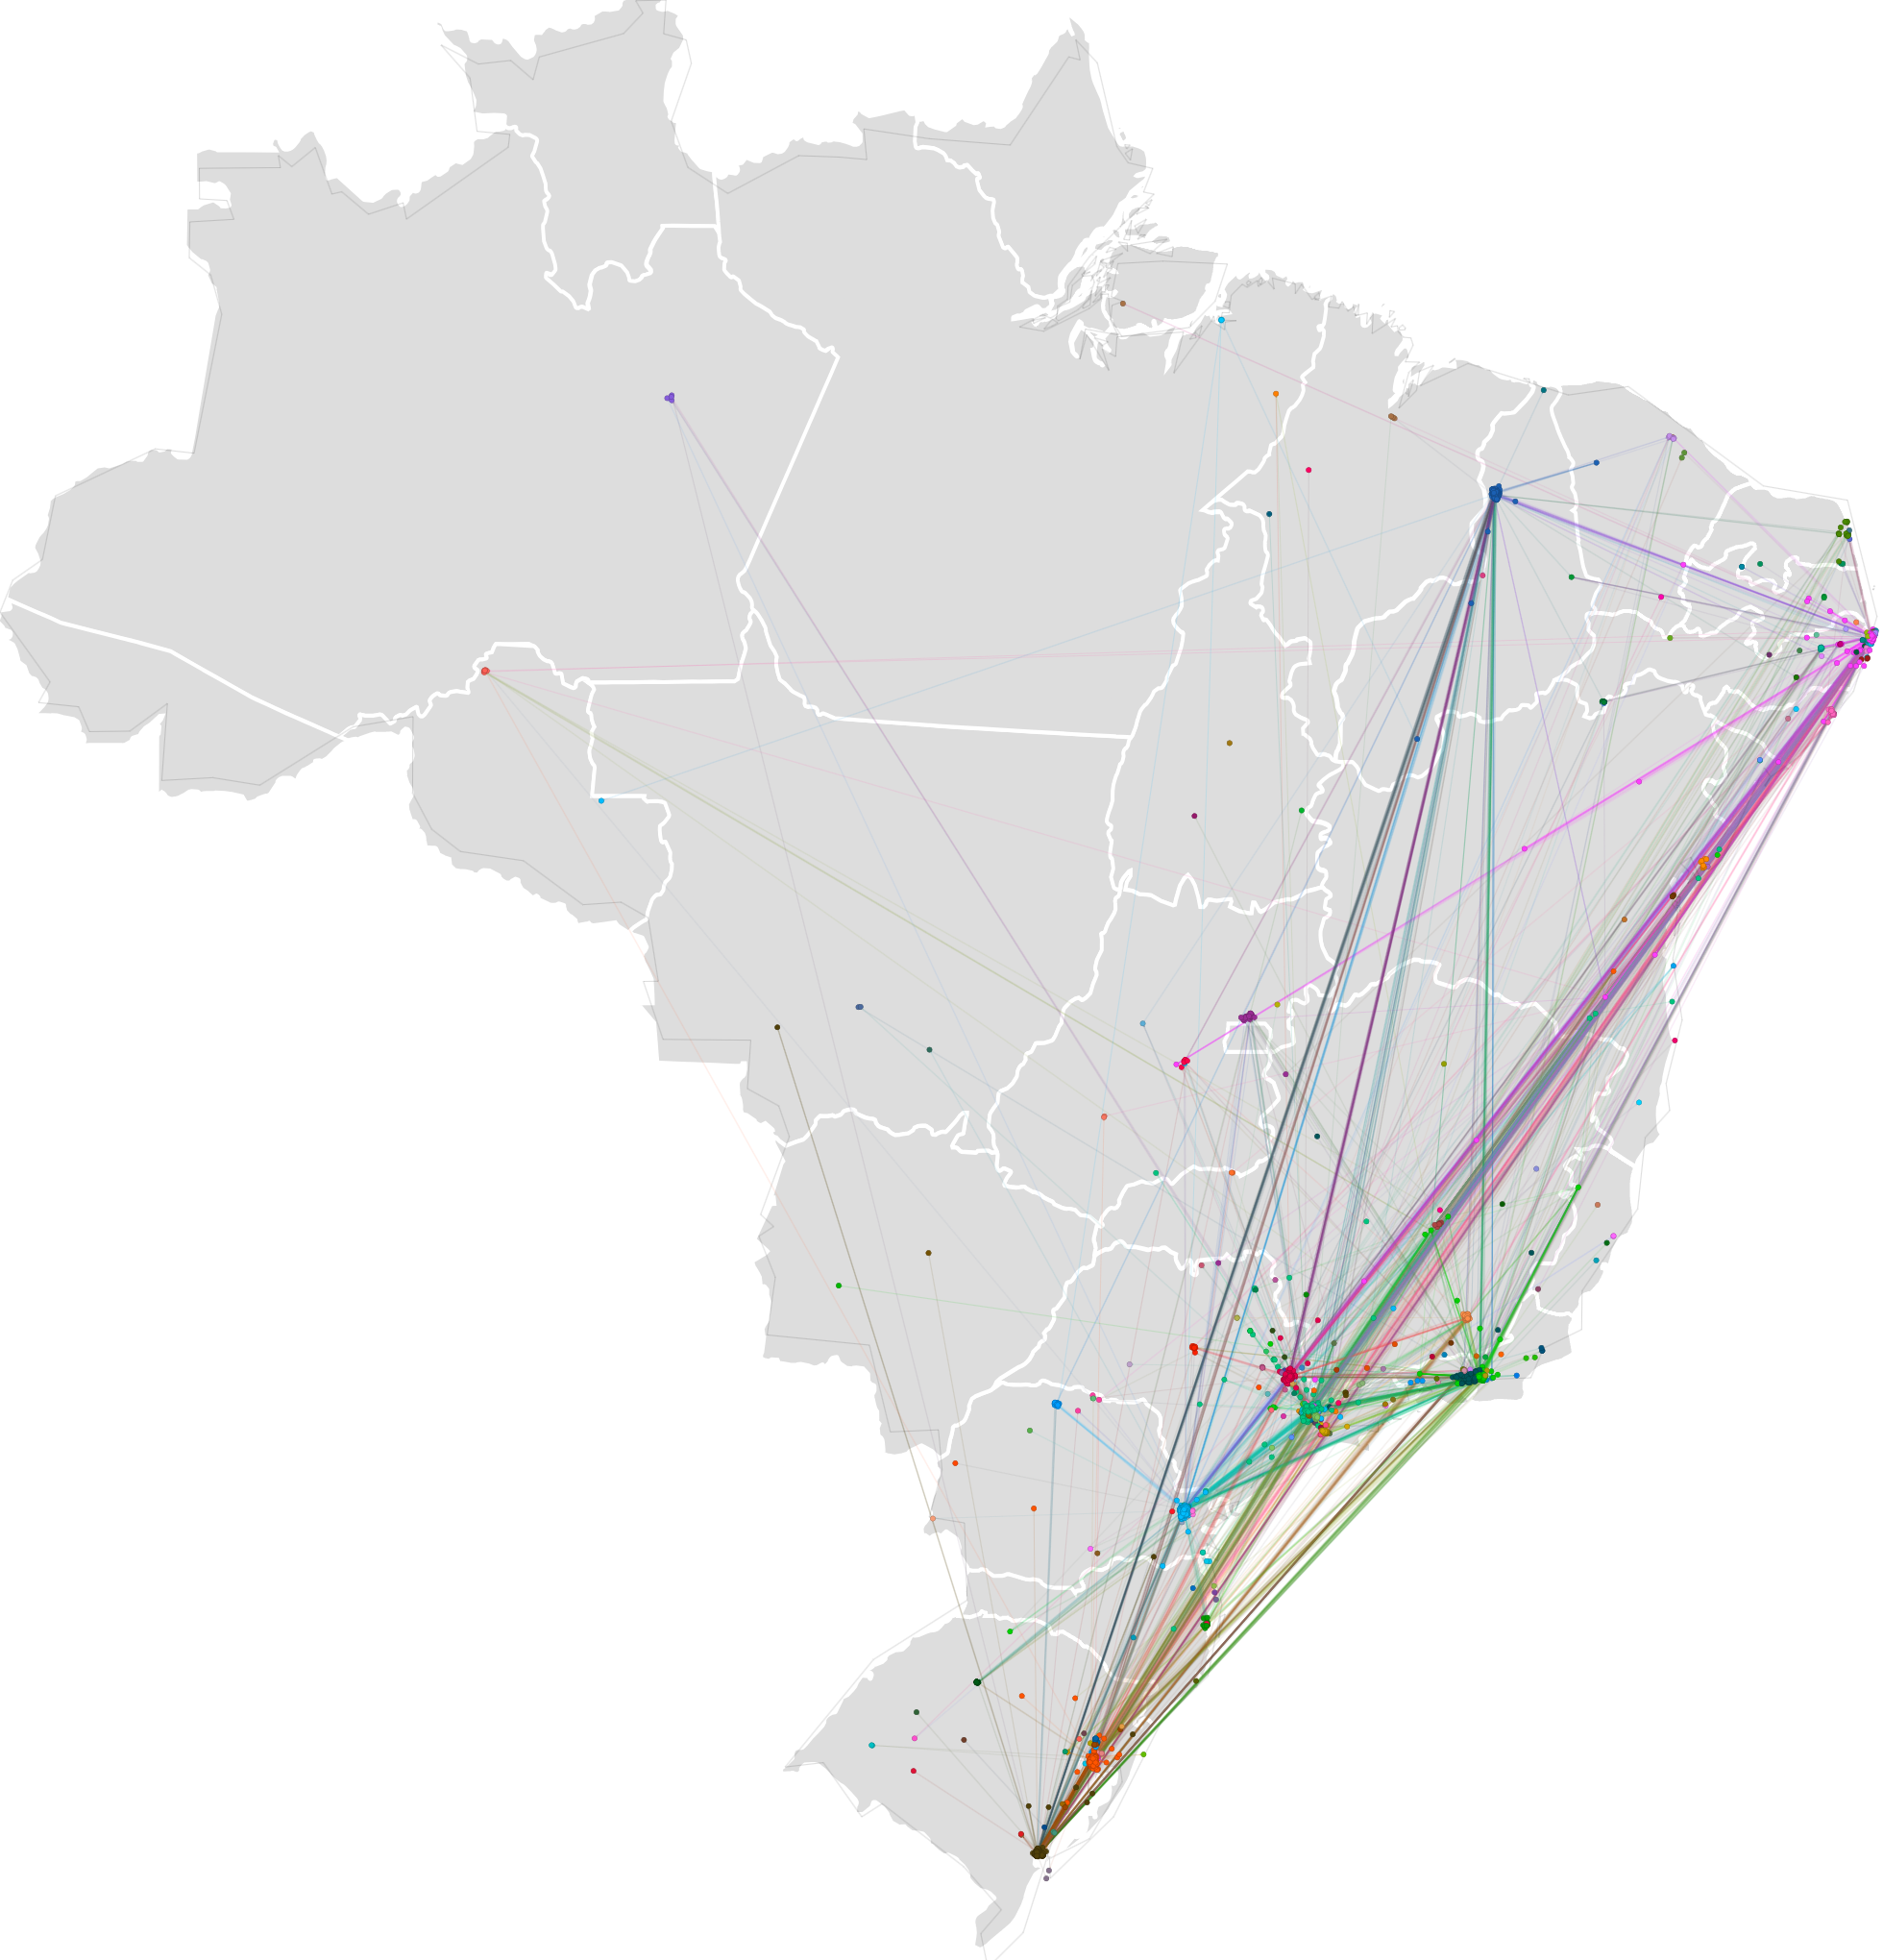
\includegraphics[scale=0.2]{images/colab-geocluster.png}
	\fautor
\end{figure}

A Figura \ref{fig:colab_geoclusters} apresenta a rede do Colab sobreposta a um mapa do Brasil, utilizando o GeoLayout do Gephi. Cada nó é colorido de acordo com o agrupamento de Louvain, e é notável que nós geograficamente próximos tendem a pertencer ao mesmo cluster. Isso sugere uma forte relação entre proximidade geográfica e formação de comunidades, reforçando o conceito de homofilia. Esta visualização também destaca as principais concentrações urbanas, permitindo uma análise mais aprofundada das dinâmicas sociais e potenciais câmaras de eco em diferentes regiões do país.

Ao nos aprofundarmos na análise da rede Colab, decidimos focar em um subset específico: os usuários das cidades de Mesquita, Niterói e Santo André. Esta granularização permite uma análise mais detalhada e contextualizada, levando em consideração as particularidades e dinâmicas sociais de cada cidade. Ao limitar nossa análise a essas cidades, podemos identificar padrões de conexão e interação que podem ser distintos em comparação com a rede geral. Esta abordagem focada aumenta a precisão na identificação de câmaras de eco, pois permite observar nuances e tendências que podem ser diluídas em uma análise de toda a rede. Além disso, ao entender as dinâmicas de câmaras de eco em níveis locais, podemos obter insights sobre como informações, crenças e valores são compartilhados e reforçados dentro de comunidades específicas, fornecendo uma base sólida para intervenções e estratégias direcionadas.

\section{Niterói, Santo André e Mesquita}

Prosseguindo com nossa investigação, decidimos concentrar nossos esforços nas cidades que apresentaram maior volume de interações no Colab. Assim, Niterói, Santo André e Mesquita emergem como os principais focos de nossa análise subsequente. Esta escolha não é aleatória, mas sim baseada na relevância e densidade de atividades nestas localidades. Ao nos concentrarmos nestas cidades, buscamos entender de forma mais precisa as dinâmicas e particularidades das interações e, consequentemente, das potenciais câmaras de eco que se formam nestes contextos específicos.

\begin{figure}[!htb]
	\caption{Rede do Colab destacando as cidades de Niterói, Santo André e Mesquita}
	\label{fig:colab_graph_3_cidades}
	\centering
	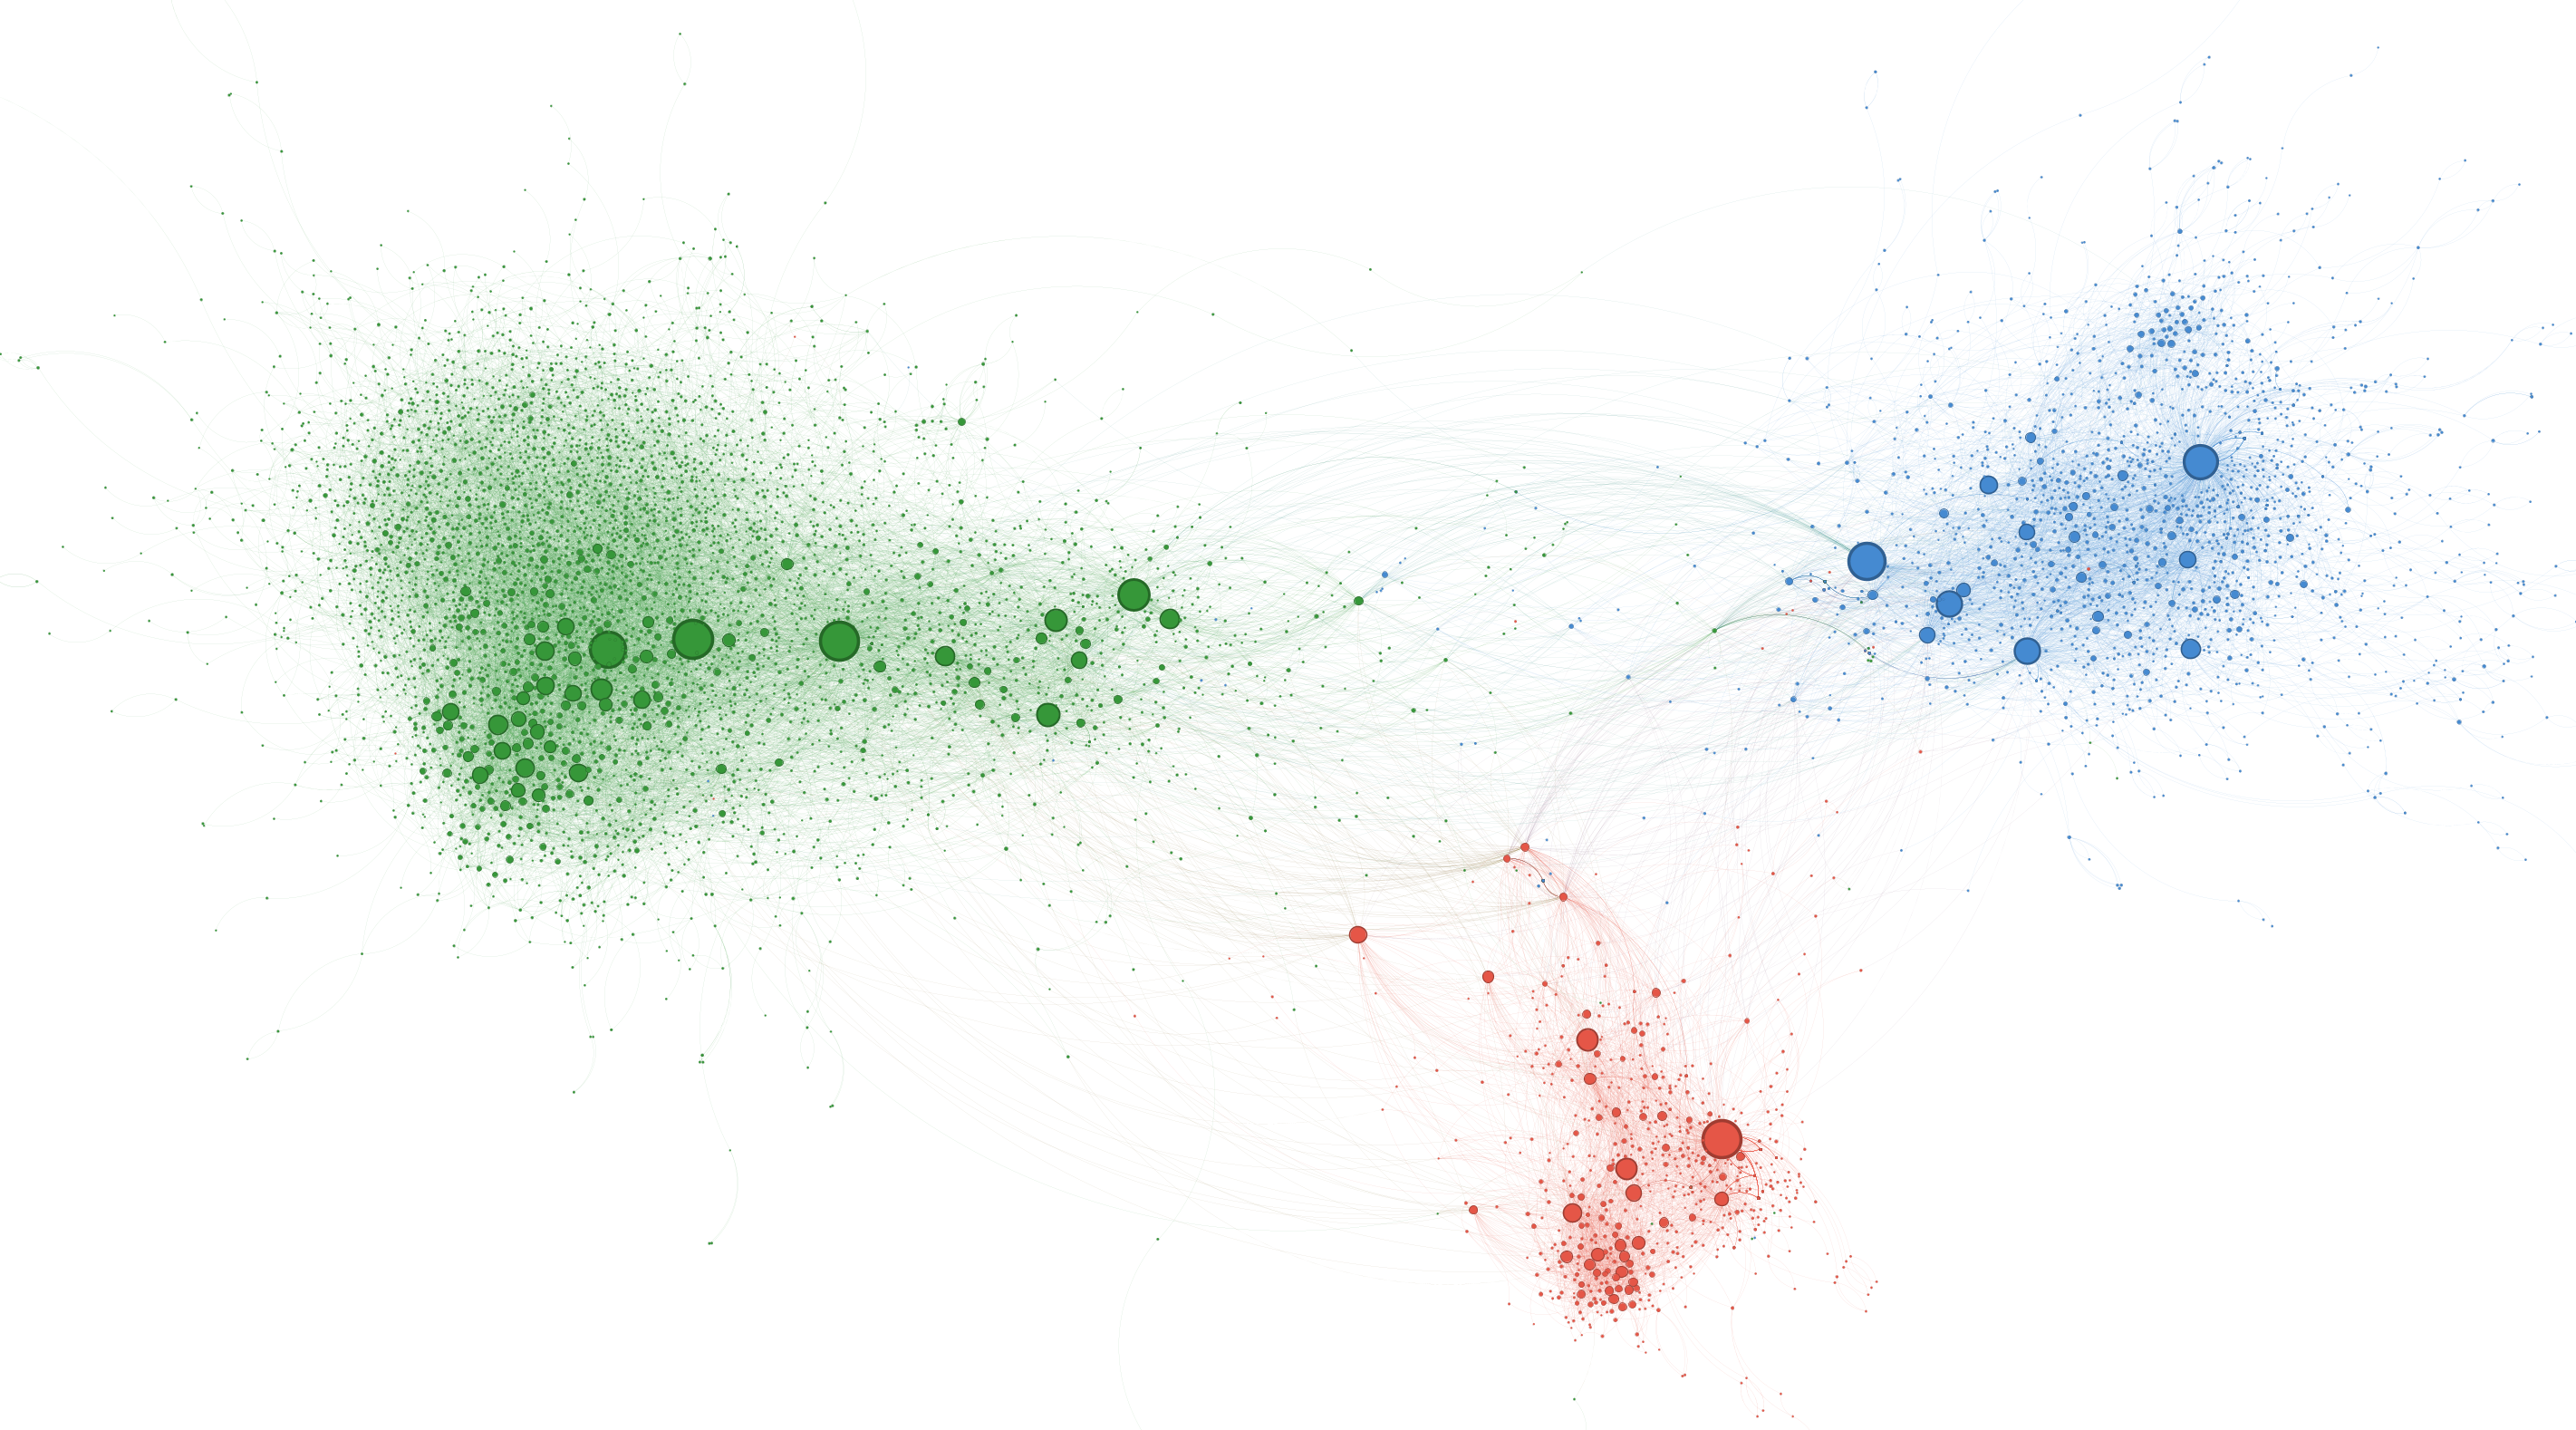
\includegraphics[scale=0.20]{images/colab_graph_3_cidades.png}
	\fautor
\end{figure}

Para iniciar, efetuamos uma filtragem dos dados, restringindo a análise aos usuários destas três cidades, resultando em uma rede composta por 6963 nós e 25785 arestas, uma redução significativa em comparação com os números iniciais de 33818 nós e 66875 arestas da rede original. Este processo de granulação permite uma análise mais focada e detalhada, facilitando a identificação de padrões e tendências específicas destas localidades.

Posteriormente, aplicamos um filtro adicional para considerar apenas os usuários com um grau de entrada maior que dois, visando eliminar nós isolados e focar em usuários com um mínimo de engajamento na rede. Além disso, focamos nossa análise no "Giant Component", que é a maior componente conectada da rede, onde existe um caminho entre cada par de nós. Este componente é crucial para entender a estrutura principal da rede, pois engloba a maior parte das interações significativas.

A coloração dos nós foi estabelecida de acordo com a cidade de origem dos usuários, adotando azul para Mesquita, rosa para Niterói e verde para Santo André, criando uma visualização que destaca a proveniência geográfica dos usuários. Adicionalmente, o tamanho dos nós foi ajustado com base no grau de entrada, representando a quantidade de seguidores, uma estratégia que realça os usuários mais influentes na rede.

Ao aplicar os layouts Force Atlas 2 e Yifan Hu, observamos uma separação natural da rede em três macro comunidades ou hubs, cada uma correlacionada a uma cidade específica. Este fenômeno evidencia um alto grau de homofilia pela localização, indicando que usuários tendem a interagir mais frequentemente com outros usuários da mesma cidade, um padrão que é corroborado em ambas as visualizações de layout, reforçando a validade desta observação.

\begin{figure}[!htb]
	\caption{Plot da rede utilizando o layout Yifan Hu.}
	\label{fig:colab_graph_3_cidades_yifan }
	\centering
	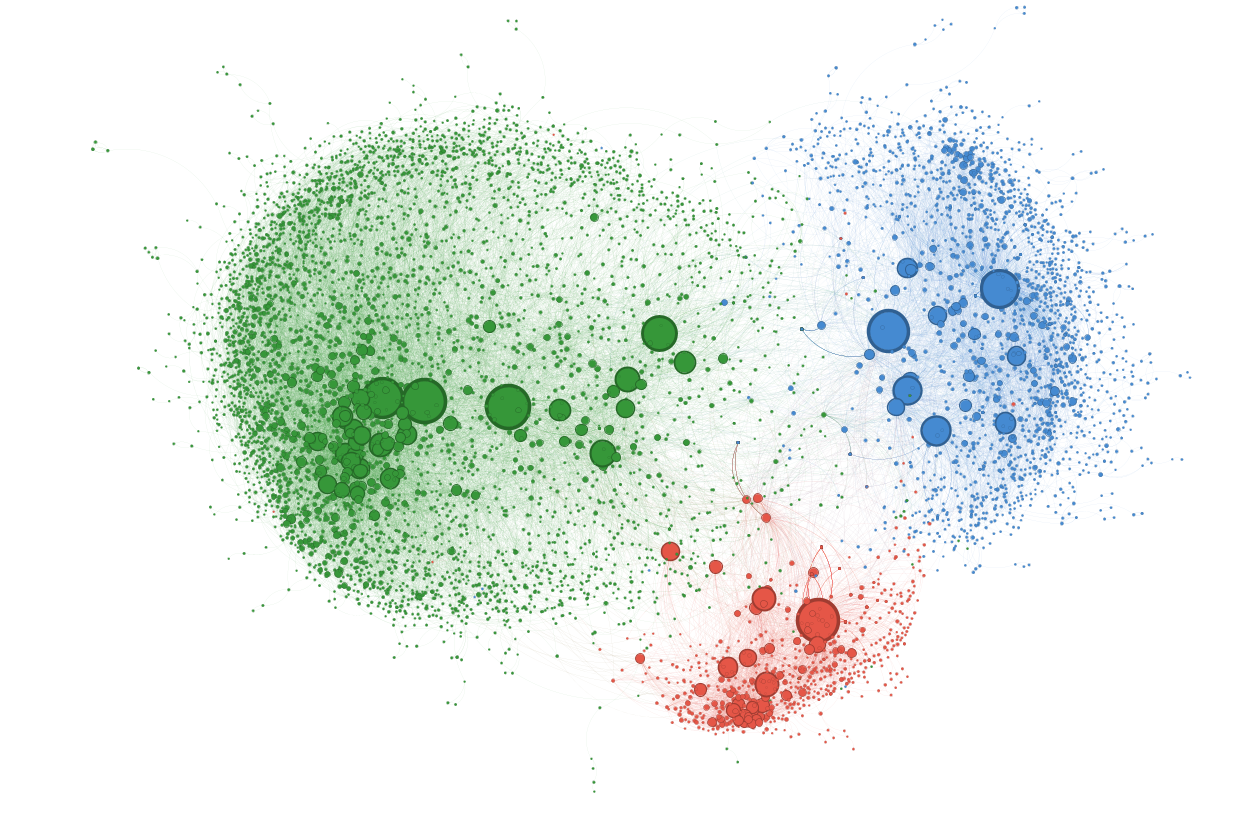
\includegraphics[scale=0.45]{images/colab_graph_3_cidades_yifan.png}
	\fautor
\end{figure}

Ao analisar as estatísticas da rede das três cidades, encontramos um grau médio de 3.703, indicando que, em média, cada usuário está conectado a aproximadamente 3-4 outros usuários. O diâmetro da rede, que é a maior distância entre dois nós, é 17, enquanto o comprimento médio do caminho é 5.318, sugerindo que, em média, são necessários pouco mais de cinco passos para conectar quaisquer dois usuários na rede. Este valor é uma indicação da eficiência da rede na disseminação de informações, onde valores menores indicam uma rede mais conectada e eficiente na transmissão de informações \cite{2010_Newman_BOOK}.

A modularidade encontrada foi de 0.519, um valor que indica uma estrutura de comunidade moderada, com uma presença significativa de grupos de usuários que estão mais densamente conectados entre si do que com o resto da rede. Este valor, juntamente com a presença de três hubs principais correlacionados com as cidades, sugere a existência de câmaras de eco geograficamente definidas, onde os usuários estão mais propensos a interagir e compartilhar informações com outros usuários de sua própria cidade, potencialmente levando a uma polarização e homogeneização de informações e perspectivas dentro dessas comunidades \cite{2010_Fortunato}.

A inferência estatística apresentou um valor de 193900.35, um indicador que, embora seja mais desafiador interpretar isoladamente, sugere uma complexidade considerável na estrutura da rede, com uma grande quantidade de comunidades distintas e padrões de conexão. Este valor, juntamente com o número significativo de componentes conectados (69 fracamente e 3927 fortemente), indica uma rede com uma estrutura complexa e multifacetada, com muitos subgrupos e comunidades interconectadas.

A centralidade de eigenvector, com uma mudança somatória de 0.015, aponta para a presença de nós influentes que desempenham um papel significativo na estrutura da rede. Estes nós, que são centrais em termos de eigenvector, podem atuar como "líderes de opinião" ou influenciadores dentro de suas respectivas comunidades, desempenhando um papel crucial na disseminação de informações e na formação de opiniões \cite{1987_Bonacich}.

Em conclusão, a análise da rede das três cidades revela uma estrutura complexa e interconectada, com padrões claros de homofilia geográfica e a presença de comunidades densamente conectadas. A combinação de visualizações de layout, métricas de rede e análises estatísticas fornece insights valiosos sobre a natureza das interações entre os usuários e as potenciais câmaras de eco que se formam dentro desta rede.

Na sequência de nossa análise, realizamos uma filtragem meticulosa dos dados no Gephi para refinar nossa visualização e focar nas interações mais significativas. Esta etapa é crucial para eliminar ruídos e destacar as estruturas subjacentes que são mais informativas. Após a filtragem, aplicamos uma coloração baseada na 'Modularidade de Classe', uma métrica que quantifica a densidade de ligações dentro das comunidades em comparação com as ligações entre comunidades. Valores altos de modularidade indicam uma divisão clara da rede em comunidades. O algoritmo de detecção de comunidades do Gephi é baseado no trabalho de \citeonline{2008_Blondel}.

\begin{table}[h]
	\centering
	\begin{tabular}{lccc}
		\hline
		\textbf{Métrica}      & \textbf{Mesquita} & \textbf{Niterói} & \textbf{Santo André} \\
		\hline
		Nodes                 & 718               & 4272             & 1973                 \\
		Edges                 & 3208              & 15751            & 6101                 \\
		Average Degree        & 4.468             & 3.687            & 3.092                \\
		Diameter              & 8                 & 16               & 13                   \\
		Average Path length   & 3.142             & 4.977            & 4.088                \\
		Modularity            & 0.310             & 0.438            & 0.411                \\
		Number of Communities & 32                & 75               & 87                   \\
		\hline
	\end{tabular}
	\caption{Estatísticas das redes das cidades de Mesquita, Niterói e Santo André.}
\end{table}

Em nossa análise de rede, priorizamos as três cidades com maior volume de interações no Colab: Niterói, Santo André e Mesquita. Avaliando a mediana dos atributos de cada cidade, Mesquita se destaca em termos de centralidade de grau e de eigenvector.

No contexto das três cidades analisadas, a métrica de modularidade revela informações cruciais sobre a estrutura da rede. Por exemplo, uma modularidade elevada sugere que a rede tem uma estrutura comunitária bem definida, o que pode ser indicativo de câmaras de eco. A detecção de comunidades e a análise da modularidade, portanto, fornecem uma lente através da qual podemos observar a formação de câmaras de eco. Em Mesquita, Niterói e Santo André, as métricas de modularidade indicam a presença de comunidades distintas. Estas comunidades, quando analisadas em detalhe, podem revelar padrões de interação que são característicos de câmaras de eco. Por exemplo, se uma comunidade particular é dominada por um único tópico de discussão ou por uma perspectiva única, isso pode ser um sinal de uma câmara de eco em ação.

Estas técnicas nos permitiram visualizar claramente as diferentes comunidades dentro de cada cidade, destacando a estrutura interna e as possíveis câmaras de eco. Em vez do algoritmo 'Force Atlas 2', optamos pelo algoritmo de layout 'Fruchterman-Reingold'. Este método, frequentemente descrito como "baseado em forças", simula uma situação em que os nós se repulsam mutuamente, como partículas carregadas negativamente, enquanto as arestas que os conectam atuam como molas, buscando manter os nós a uma distância desejada. O algoritmo move os nós de acordo com essas forças até que um equilíbrio seja alcançado, proporcionando uma representação visual clara e intuitiva das comunidades e suas inter-relações.

\begin{figure}[h]
    \centering
    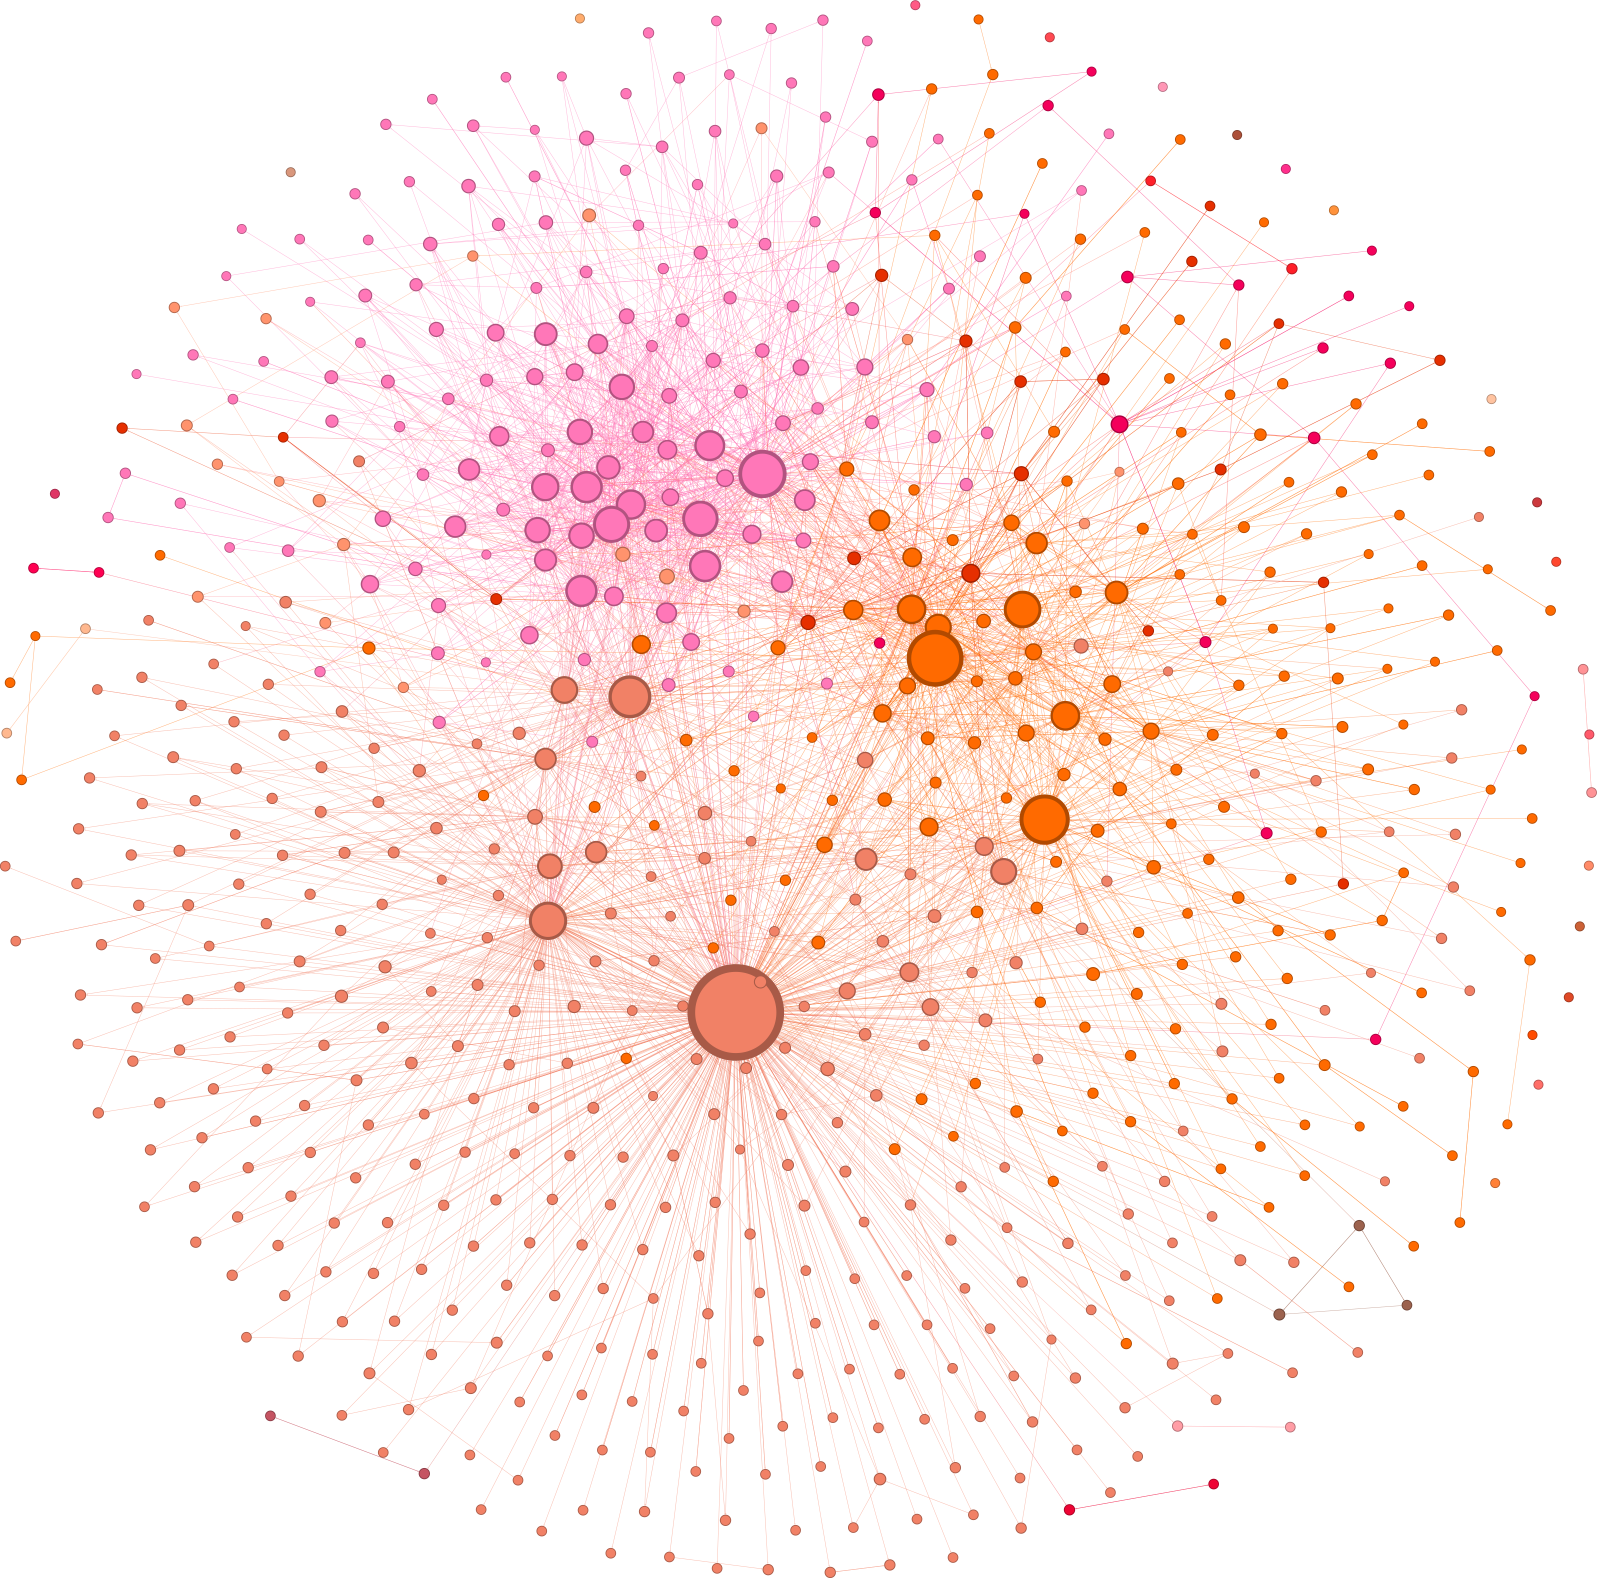
\includegraphics[width=0.8\textwidth]{images/graph-mesquita.png}
    \caption{Visualização da rede da cidade de Mesquita. O layout foi gerado usando o algoritmo Fruchterman-Reingold e o agrupamento foi realizado com o método de Louvain.}
    \label{fig:mesquita-graph}
	\fautor
\end{figure}

Na cidade de Mesquita, a rede é composta por 718 nós e 3208 arestas, com um grau médio de 4.468. O diâmetro da rede é de 8, indicando que o caminho mais longo entre dois nós é de 8 arestas. A métrica de 'Modularidade' é de 0.310, sugerindo uma presença moderada de comunidades dentro da rede. A detecção de comunidades revelou 32 comunidades, enquanto a inferência estatística sugere a existência de 75 comunidades. Esta discrepância pode ser devido a diferentes métodos de detecção de comunidades ou a presença de subcomunidades dentro das principais comunidades identificadas. A presença de 21 componentes fracamente conectados e 315 componentes fortemente conectados indica que, embora existam muitos grupos isolados, a maioria dos nós está fortemente interconectada.

\begin{figure}[h]
    \centering
    \includegraphics[width=0.8\textwidth]{images/graph-niteroi.png}
    \caption{Visualização da rede da cidade de Niterói. O layout foi gerado usando o algoritmo Fruchterman-Reingold e o agrupamento foi realizado com o método de Louvain.}
    \label{fig:niteroi-graph}
	\fautor
\end{figure}

Em Niterói, a rede é significativamente maior, com 4272 nós e 15751 arestas. O grau médio é de 3.687, e o diâmetro da rede é de 16. A 'Modularidade' é de 0.438, indicando uma presença mais forte de comunidades em comparação com Mesquita. Foram identificadas 75 comunidades, e a inferência estatística sugere a presença de 316 comunidades. O coeficiente de agrupamento médio é de 0.086, o que sugere que os nós tendem a criar triângulos ou tríades. Esta métrica é importante porque indica a tendência dos nós de formar grupos fechados, o que pode ser um indicativo da formação de câmaras de eco.

\begin{figure}[h]
    \centering
    \includegraphics[width=0.8\textwidth]{images/graph-santo-andre.png}
    \caption{Visualização da rede da cidade de Santo André. O layout foi gerado usando o algoritmo Fruchterman-Reingold e o agrupamento foi realizado com o método de Louvain.}
    \label{fig:santo-andre-graph}
	\fautor
\end{figure}

Santo André apresenta uma rede com 1973 nós e 6101 arestas. O grau médio é de 3.092, e o diâmetro da rede é de 13. A 'Modularidade' é de 0.411, sugerindo uma presença forte de comunidades. Foram identificadas 87 comunidades, enquanto a inferência estatística sugere a existência de 164 comunidades. O coeficiente de agrupamento médio é de 0.220, o que é significativamente maior do que em Niterói, indicando uma maior tendência dos nós em Santo André de formar grupos fechados.

A detecção de comunidades é uma área de pesquisa em rápido crescimento, com aplicações em várias disciplinas, desde a biologia até as ciências sociais. Segundo \citeonline{2010_Fortunato}, a capacidade de identificar comunidades em redes complexas permite uma melhor compreensão da estrutura e função dessas redes. Em relação às câmaras de eco online, \citeonline{2016_Vicario} destacam que as redes sociais online podem amplificar a polarização e a segregação, levando à formação de câmaras de eco onde os usuários são expostos principalmente a informações que reforçam suas crenças preexistentes.

A presença de comunidades densamente conectadas e a formação de câmaras de eco são fenômenos inter-relacionados. As comunidades tendem a formar-se em torno de interesses ou opiniões comuns, e dentro dessas comunidades, os membros são mais propensos a interagir com informações que confirmam suas crenças, levando à formação de câmaras de eco. Este fenômeno é exacerbado pelas plataformas de mídia social que utilizam algoritmos de recomendação para mostrar aos usuários conteúdo que é provável que eles achem interessante ou concordem, reforçando ainda mais as câmaras de eco.

Ao examinar a estrutura da rede em Mesquita, observamos um padrão distintivo: um usuário em particular emerge como uma figura central, atuando como um hub com múltiplas conexões irradiando a partir dele. Em contraste, Santo André exibe uma configuração mais fragmentada, caracterizada por diversos núcleos descentralizados. Niterói, contudo, diverge desses padrões, manifestando uma rede compacta e coesa, onde as conexões são densamente entrelaçadas.

Ao mergulhar nas métricas da rede, notamos que Mesquita ostenta uma predominância de usuários cujo eigenvector é marginalmente elevado. Em contrapartida, tanto Santo André quanto Niterói apresentam uma distribuição onde a maioria dos usuários tem um eigenvector aproximando-se de zero.

Em uma perspectiva sobre a demografia dos usuários, correlacionando-os com o valor do eigenvector percebe-se que em Niterói, uma demografia mais jovem é evidente, uma característica que não é tão proeminente em Mesquita ou Santo André. Em uma observação mais ampla, os usuários que detêm uma centralidade elevada tendem a ter idades entre 31 e 64 anos.

Explorando ainda mais a arquitetura das redes, nos deparamos com o conceito de excentricidade. Esta métrica delineia a distância máxima entre um nó específico e todos os demais na rede. Em termos mais coloquiais, a excentricidade de um nó representa a distância mais longa, contada pelo número de arestas, que se deve percorrer para alcançar esse nó a partir de qualquer outro ponto da rede.

A investigação da rede social Colab desvelou nuances sobre a dinâmica e o perfil dos usuários. Uma constatação notável é que a vasta maioria dos usuários mantém até 10 conexões, tendo registrado até 10 comentários e 10 curtidas.

Ao focar nos usuários mais proeminentes, identificamos uma demografia que oscila entre 37 e 52 anos. Globalmente, a plataforma é dominada por indivíduos do sexo masculino, de etnia branca e com formação acadêmica avançada.

Ao segmentar os usuários em cinco clusters através do K-means, percebemos que Mesquita e Santo André exibem padrões distributivos análogos, enquanto Niterói se distingue com um cluster particularmente proeminente. Notavelmente, o cluster composto por indivíduos de maior influência permeia as três cidades, com uma representatividade mais acentuada em Mesquita.

Em um esforço para mapear a distribuição geográfica dos clusters, não identificamos aglomerações em áreas específicas das cidades.

Ao focar exclusivamente nas conexões entre usuários, geramos visualizações das redes. Em Mesquita, uma concentração de usuários em torno de um indivíduo é patente, com o restante da rede apresentando-se mais disperso. Em Santo André, a rede é pontuada por diversos núcleos menores. Em Niterói, a representação gráfica revela uma rede intrincada e coesa.

Concluindo, nossa incursão na análise da rede social do Colab nos brindou com insights profundos sobre as interações dos usuários, a dinâmica da plataforma e os perfis dos usuários mais influentes. Estes achados iniciais sobre a rede Colab são cruciais para orientar aprimoramentos na plataforma, potencializar a interação entre os usuários, conceber estratégias de comunicação mais eficazes e prover informações valiosas aos stakeholders.

À luz da metodologia de \citeonline{2023_Atiqi_BOOK}, a topologia das redes das 3 cidades, sugere a presença de subgrupos ou comunidades que podem funcionar como câmaras de eco. Estas são áreas da rede onde os membros estão fortemente alinhados em suas opiniões ou informações compartilhadas. A presença de múltiplos componentes fortemente conectados em cada cidade indica que, enquanto há muita interconexão, também existem bolsões isolados de opinião. Estes bolsões podem ser áreas onde as opiniões são reforçadas sem exposição a perspectivas divergentes, um indicativo clássico de câmaras de eco. A modelagem baseada em agentes, como proposto por Atiqi, pode ajudar a entender melhor como as informações se propagam nessas redes e como as câmaras de eco se formam e persistem.

Em conclusão, a análise das redes das três cidades revela padrões distintos de interconexão e formação de comunidades. A presença de comunidades densamente conectadas sugere a possibilidade de câmaras de eco, onde os membros são expostos a um conjunto limitado de informações que reforçam suas crenças preexistentes. Esta análise destaca a importância de compreender a estrutura e dinâmica das redes sociais para abordar os desafios associados à polarização e segregação online.

\subsection*{Limitações do algoritmo de Louvain}
\label{sec:limitacoes_louvain}

É importante destacar que o algoritmo de Louvain foi originalmente desenvolvido para redes não direcionadas. No entanto, muitas redes reais, incluindo a rede que estamos analisando neste estudo, são direcionadas. Neste contexto, uma questão pertinente surge: como o Gephi, que utiliza o algoritmo de Louvain, lida com redes direcionadas?

Ao analisar o código fonte \cite{2011_McSweeney} e os relatórios gerados pelo Gephi, observa-se que a ferramenta parece converter redes direcionadas em não direcionadas para a aplicação do algoritmo de Louvain. Essa abordagem, embora permita a utilização de uma metodologia consolidada de detecção de comunidades, pode não capturar completamente a estrutura e as nuances de uma rede direcionada. Por exemplo, relações de autoridade, hierarquia ou influência, que são intrínsecas a redes direcionadas, podem ser perdidas durante essa conversão.

Além da metodologia de Louvain tradicionalmente aplicada a redes não direcionadas, é essencial considerar a dinâmica e a estrutura modular em múltiplas escalas em redes. \citeonline{2008_Lambiotte} destaca que muitas redes são inerentemente modulares, o que significa que elas consistem em módulos ou comunidades. A estabilidade, definida pelas propriedades estatísticas de um caminhante aleatório movendo-se no gráfico, é usada como uma medida para determinar a qualidade de uma partição. Uma observação crítica é que a estabilidade da partição de um gráfico muda com o tempo, permitindo uma compreensão em várias escalas das comunidades em redes. No entanto, uma consideração crucial é que a modularidade e a estabilidade são fundamentalmente diferentes no caso de redes direcionadas. Isso sugere que, ao aplicar métodos como o de Louvain a redes direcionadas, como as encontradas em muitos contextos de mídia social, é vital considerar essas diferenças e as implicações metodológicas resultantes.

\subsection*{Alternativas em detecção de comunidades}

Ao abordar redes direcionadas, é crucial considerar a direcionalidade das arestas. Como discutido por \citeonline{2013_Malliaros}, ignorar essa direcionalidade pode levar à perda de semântica subjacente. Em muitos casos, essa simplificação não seria satisfatória, especialmente em redes onde a direcionalidade tem um significado significativo. Além disso, a presença de arestas direcionadas implica a possibilidade de tipos mais sofisticados de clusters que representam padrões de movimento ou circulação de fluxo entre os nós. Portanto, ao aplicar métodos como o Louvain em redes direcionadas, é essencial adaptar e considerar essas nuances para garantir que as comunidades detectadas sejam verdadeiramente representativas da estrutura da rede.

Uma alternativa ao cálculo de modularidade padrão do Gephi é o algoritmo de Girvan-Newman, proposto por \cite{2002_Girvan}. Este algoritmo é baseado na ideia de que uma aresta entre duas comunidades tem, provavelmente, menos ligações do que uma aresta dentro de uma comunidade. Assim, ao remover iterativamente as arestas com a maior centralidade de intermediação (ou "betweenness"), as comunidades emergem naturalmente como componentes desconexos. O algoritmo é particularmente eficaz em redes com estrutura hierárquica de comunidades e tem sido amplamente utilizado em diversos campos de pesquisa.

Através de um plugin para o Gephi, é possivel aplicar o algoritmo de Girvan-Newman à rede de Mesquita, por exemplo, encontramos um total de 67 comunidades, com uma modularidade máxima de 0.3027. Em contraste, o cálculo de modularidade padrão do Gephi identificou 26 comunidades com uma modularidade de 0.431. A diferença na quantidade de comunidades e nos valores de modularidade sugere que os dois métodos têm diferentes sensibilidades à estrutura da rede. No contexto da nossa pesquisa sobre câmaras de eco, a escolha do método pode depender do foco da análise. Se estivermos interessados em identificar um maior número de comunidades potencialmente menores e mais coesas, o algoritmo de Girvan-Newman pode ser mais apropriado. No entanto, se buscarmos uma visão mais macroscópica das principais comunidades na rede, a abordagem de modularidade padrão do Gephi pode ser preferível. Ambos os métodos oferecem insights valiosos, e a escolha pode ser guiada pelo objetivo específico da análise e pela natureza da rede em estudo.

O algoritmo Leiden, uma extensão avançada do método de Louvain, é uma abordagem contemporânea para detecção de comunidades em redes \cite{2018_Traag}. Desenvolvido para superar certas limitações do Louvain, o Leiden opera através de um processo iterativo de particionamento local, refinamento e agregação, garantindo uma partição de alta qualidade ao otimizar a modularidade da rede. Em nossa análise para a cidade de Mesquita, utilizando o algoritmo Leiden com a função de qualidade baseada em modularidade e uma resolução de 1.0 ao longo de 100 iterações, obtivemos uma modularidade de 0.4441 e identificamos 30 comunidades distintas. Em comparação com os resultados anteriores, o Leiden apresentou uma modularidade ligeiramente superior ao método padrão do Gephi (0.431) e identificou um número de comunidades que se situa entre o método padrão do Gephi (26 comunidades) e o Girvan-Newman (67 comunidades). Essa variação nos resultados destaca a sensibilidade dos diferentes algoritmos à estrutura da rede e reforça a importância de considerar múltiplas abordagens ao analisar comunidades em redes complexas.

No entanto, a pesquisa está avançando para superar essa limitação. O estudo de \citeonline{2015_Dugue} introduz uma extensão do método de Louvain para redes direcionadas, preservando a direcionalidade das conexões na análise de comunidades. Essa abordagem, denominada DirectedLouvain, maximiza uma função objetivo de modularidade direcionada, permitindo a detecção de comunidades em redes com links direcionados. A implementação dessa metodologia pode oferecer insights mais profundos sobre a estrutura da rede, mantendo a riqueza de informações contida nas direções dos links. Assim, para estudos futuros, seria interessante explorar a aplicação do DirectedLouvain para uma análise mais refinada das câmaras de eco, levando em consideração a direcionalidade das conexões na rede.

\section{Abordagem programática}

\begin{figure}[h]
    \centering
    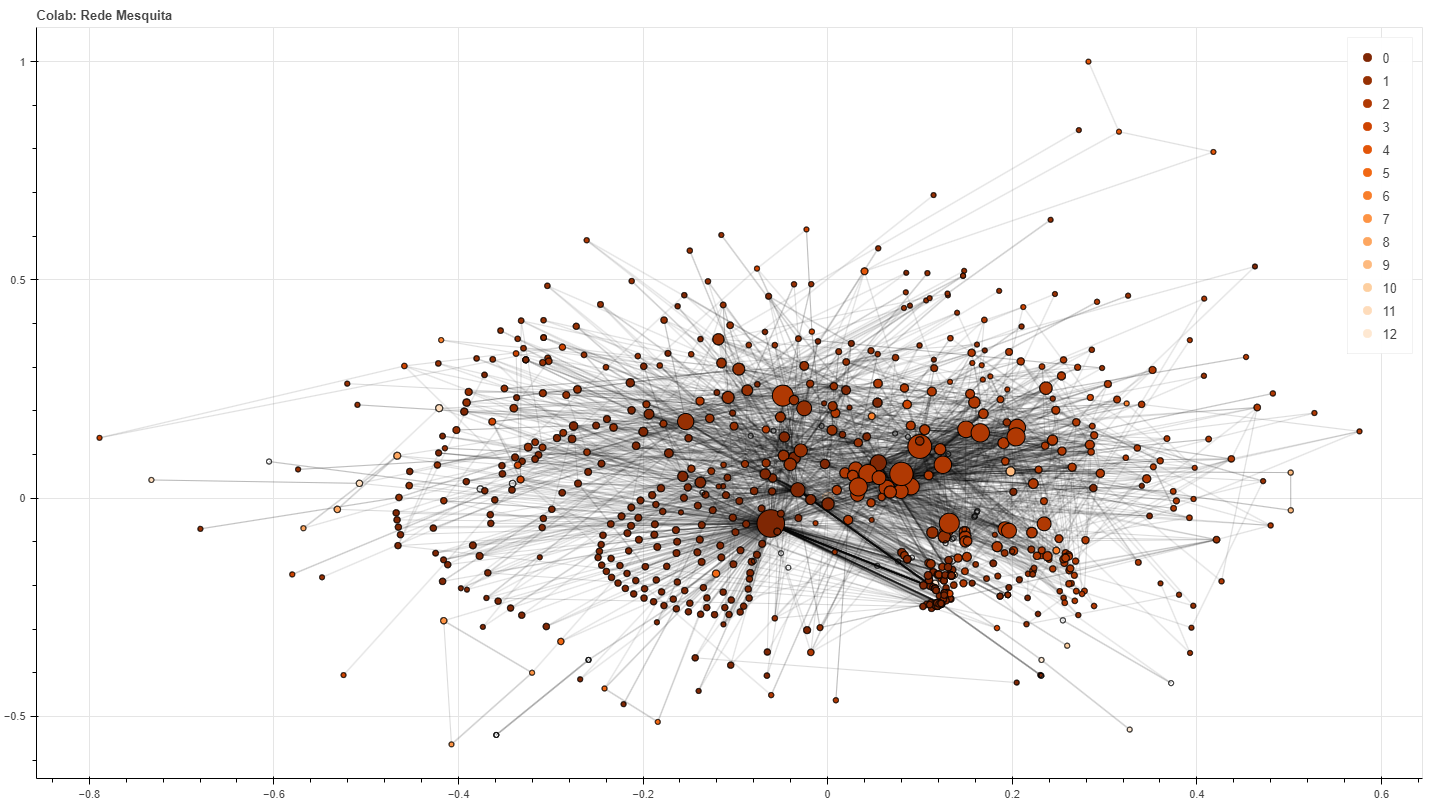
\includegraphics[scale=0.30]{images/bokeh_plot.png}
    \caption{Visualização interativa da rede Colab na cidade de Mesquita utilizando a biblioteca Bokeh. Layout aplicado: Kamada-Kawai.}
    \label{fig:bokeh_plot}
	\fautor
\end{figure}

Durante nossa análise exploratória da rede social do Colab, inicialmente optamos por utilizar a ferramenta Gephi para visualização e análise dos dados. Utilizando o Gephi, conseguimos identificar algumas características interessantes da rede, como agrupamentos e centralidades. No entanto, conforme a complexidade da rede aumentava, percebemos que o processo de análise manual no Gephi se tornava mais desafiador e demorado. Além disso, a reprodução dos passos de análise no Gephi era difícil de compartilhar e replicar. Por fim, como discutido acima, as heurísticas de modularidade do Gephi não são adequadas para redes direcionadas, o que não é neccessariamente um problema em uma análise a nível exploratório, mas que pode ser relevante ao se tratar de heurísticas para detecção de câmaras de eco baseado em comunidades de um grafo.

Para superar essas limitações, decidimos incorporar uma abordagem baseada em código em nossa análise. Isso nos permitiu automatizar várias etapas do processo de análise, proporcionando uma maior flexibilidade e eficiência. Em particular, desenvolvemos uma classe chamada NetworkPlotter em Python, que nos permitiu realizar análises mais avançadas e explorar diferentes métricas de SNA.

A abordagem baseada em código nos trouxe diversos benefícios em relação ao uso do Gephi. Em primeiro lugar, a automação das etapas de análise nos permitiu trabalhar com redes maiores e mais complexas, que seriam impraticáveis de analisar manualmente no Gephi. Além disso, a flexibilidade do código nos permitiu ajustar e personalizar as análises de acordo com nossas necessidades específicas. Também pudemos criar visualizações interativas dos resultados, permitindo uma exploração mais profunda da rede.

A classe NetworkPlotter foi essencial nesse processo. Ela encapsula a lógica para a visualização e análise de redes complexas, utilizando bibliotecas como NetworkX e Bokeh. A classe nos permite calcular métricas de grau e centralidade, normalizar tamanhos de nós e criar visualizações interativas do grafo. Essa abordagem orientada a código nos forneceu uma ferramenta poderosa e reutilizável para análise de redes sociais, facilitando a exploração e compreensão da estrutura e dinâmica da rede do Colab.

Iniciando com a métrica de grau, é utilizado o método \texttt{nx.degree()} para calcular o grau de cada nó, representando o número de conexões de entrada ou saída do mesmo. Essa métrica permite identificar nós importantes dentro da rede, uma vez que nós com um alto grau estão mais conectados a outros nós e podem desempenhar papéis de influência significativos.

Além disso, o código emprega o algoritmo \texttt{nx.eigenvector\_centrality\_numpy()} para calcular a centralidade de cada nó. A centralidade de um nó mede sua importância relativa com base em sua posição e conexões no grafo. Nesse caso, o algoritmo de centralidade de eigenvector é utilizado para considerar tanto as conexões diretas de um nó quanto a importância dos nós vizinhos. Dessa forma, a centralidade pode ser interpretada como um indicador de influência ou prestígio dentro da rede.

Uma etapa adicional do código é a normalização do tamanho dos nós, realizada por meio da função \texttt{normalize()}. Essa normalização tem como objetivo ajustar visualmente os tamanhos dos nós com base em limites desejados e atuais, visando uma representação adequada no gráfico de rede. Essa técnica permite destacar visualmente os nós mais importantes com base em suas métricas de grau e centralidade, facilitando a análise e interpretação dos resultados.

\begin{figure}[h]
    \centering
    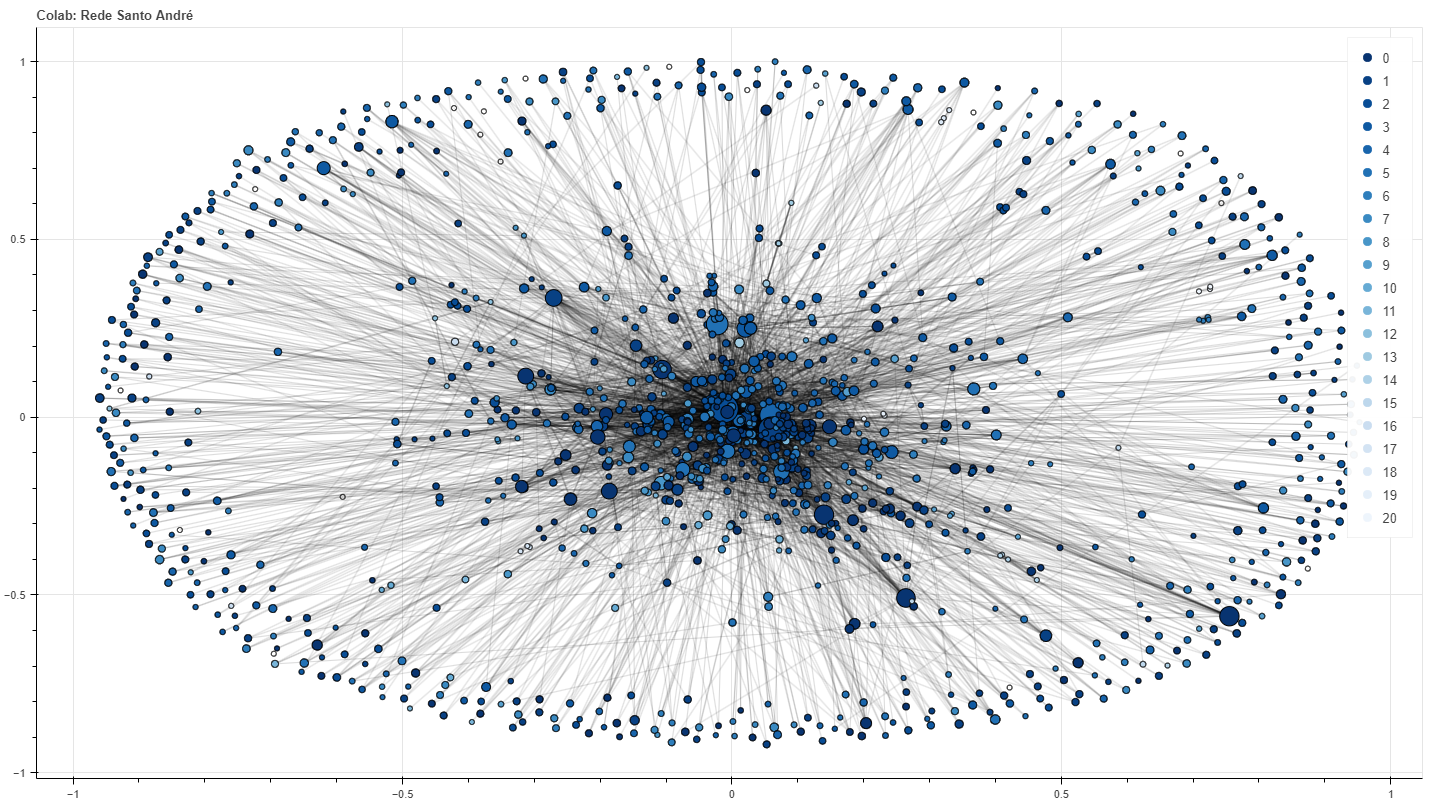
\includegraphics[scale=0.3]{images/bokeh_plot_santo_andre.png}
    \caption{Visualização interativa da rede Colab na cidade de Santo André com o layout spring, o padrão da biblioteca NetworkX.}
    \label{fig:bokeh_plot_santo_andre}
	\fautor
\end{figure}

Como ja discutido em \autoref{sec:limitacoes_louvain}, a detecção de comunidades em grafos direcionados é uma questão delicada que exige alguns benchmarks. Ao explorar diferentes métodos de detecção de comunidades, observamos variações significativas nos resultados, refletindo as diferentes abordagens e heurísticas que cada algoritmo utiliza. A abordagem de Louvain, por exemplo, identificou 116 comunidades na rede da cidade de Mesquita, com a maior comunidade composta por 118 nós e a menor por apenas um nó. A média de tamanho da comunidade foi de aproximadamente 6,19 nós, e o score de modularidade foi de 0,3574.

Por outro lado, o algoritmo de modularidade gananciosa \cite{2004_Clauset} identificou 40 comunidades, com a maior comunidade contendo 333 nós e a menor apenas um nó. A média de tamanho da comunidade foi significativamente maior, com cerca de 17,95 nós por comunidade, e um score de modularidade de 0,4297. No entanto, é importante observar que comunidades com apenas um ou dois nós podem não ser representativas ou significativas em muitos contextos de análise de redes sociais. Portanto, como etapa de pré-processamento, optamos por considerar apenas as comunidades que continham no mínimo 3 usuários. Esse critério visa garantir que as comunidades identificadas sejam robustas e tenham relevância prática, evitando a inclusão de pequenos agrupamentos que podem surgir devido a ruídos ou conexões esporádicas na rede. Ao aplicar esse filtro, o número total de comunidades e a distribuição de seus tamanhos podem variar, mas a análise resultante tende a ser mais focada em agrupamentos significativos e bem definidos na rede.

Comparando com os resultados obtidos no Gephi, que identificou 25 comunidades e obteve um score de modularidade de 0,426, podemos inferir algumas observações. Primeiramente, o algoritmo de Louvain tende a identificar um maior número de comunidades menores, enquanto o algoritmo de modularidade gananciosa identifica menos comunidades, mas de tamanho maior. O Gephi, com sua abordagem padrão, situa-se entre esses dois extremos em termos de número de comunidades e score de modularidade.

\begin{figure}[h]
    \centering
    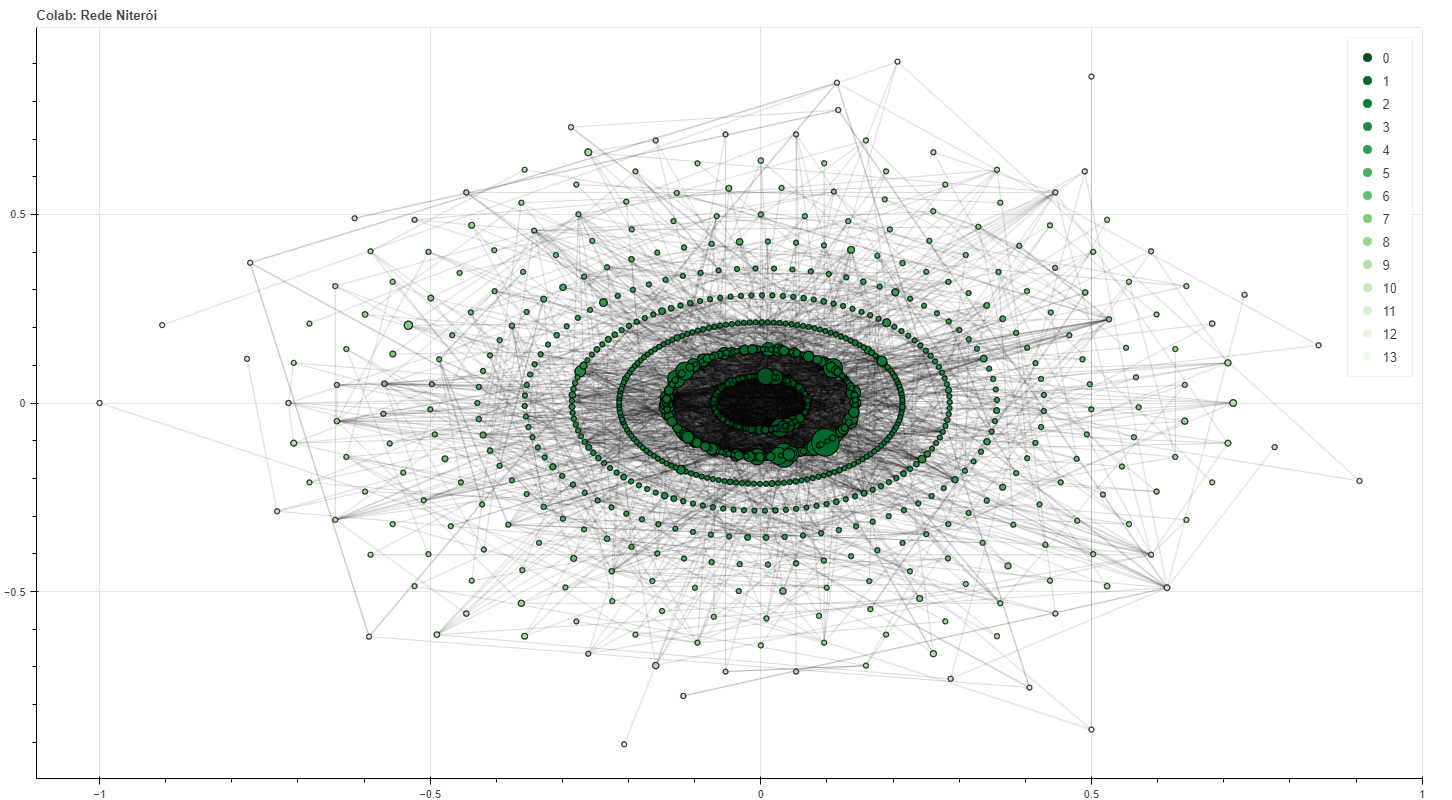
\includegraphics[scale=0.3]{images/bokeh_plot_niteroi.png}
    \caption{Visualização interativa da rede Colab na cidade de Niterói com o layout shell, exibindo as comunidades como órbitas.}
    \label{fig:bokeh_plot_niteroi}
	\fautor
\end{figure}

No contexto da nossa pesquisa sobre câmaras de eco, a escolha do algoritmo de detecção de comunidades pode influenciar significativamente nossas conclusões. Comunidades menores, como as identificadas pelo algoritmo de Louvain, podem indicar grupos mais coesos e isolados, que são características típicas de câmaras de eco. Por outro lado, comunidades maiores, como as identificadas pelo algoritmo de modularidade gananciosa, podem representar grupos mais diversificados e interconectados.

A classe \texttt{NetworkPlotter} em nossa abordagem programática é agnóstica quanto ao método de detecção de comunidades, permitindo flexibilidade na escolha do algoritmo. Isso é crucial para uma análise robusta, pois nos permite comparar e contrastar resultados de diferentes algoritmos e escolher aquele que melhor se adapta ao nosso contexto e objetivos de pesquisa.

A disposição espacial dos nós em uma visualização de rede, conhecida como layout, é crucial para a interpretação intuitiva da estrutura da rede. Diferentes estratégias de layout podem revelar diferentes aspectos da rede, desde agrupamentos locais até a estrutura global. A classe \texttt{NetworkPlotter} suporta diferentes layouts através do design pattern \textit{strategy}. O layout Kamada-Kawai, que optamos por utilizar, é uma técnica baseada em um modelo de molas. Neste modelo, os nós são tratados como partículas carregadas que se repelem mutuamente, enquanto as arestas são tratadas como molas que tentam manter os nós a uma distância desejada um do outro. O objetivo é encontrar uma disposição que minimize a energia do sistema, resultando em uma representação visual equilibrada da rede. Esta abordagem foi introduzida por \citeonline{1989_Kamada}. A escolha deste layout para nossa visualização foi motivada por sua capacidade de produzir representações claras e bem distribuídas de redes complexas, facilitando a identificação de agrupamentos e relações entre os nós.

Para facilitar a visualização e exploração da rede, o código utiliza a biblioteca Bokeh para criar um gráfico interativo. O gráfico resultante exibe os nós e suas conexões, com tamanhos e cores que refletem as métricas de interesse. Além disso, a inclusão das comunidades do grafo proporciona uma análise mais aprofundada da estrutura e organização da rede, permitindo a identificação de agrupamentos ou módulos.

Em resumo, o código implementa uma abordagem de ARS com ênfase na análise de grafos, métricas de grau e centralidade, normalização de tamanho de nós e visualização interativa. Essa combinação de técnicas e algoritmos fornece uma plataforma flexível para explorar redes sociais complexas, identificar nós de destaque e compreender a estrutura e dinâmica da rede em estudo.

Apesar das visualizações bidimensionais serem amplamente utilizadas e oferecerem insights valiosos sobre a estrutura da rede, elas têm suas limitações, especialmente quando se trata de redes de grande escala e densamente conectadas. Nestes casos, uma representação bidimensional pode não ser suficiente para capturar e representar adequadamente todas as nuances e complexidades da rede. É aqui que a visualização em três dimensões (3D) entra em cena, abrindo um novo horizonte de possibilidades para a análise e interpretação de estruturas complexas. A capacidade de explorar uma rede em 3D oferece uma perspectiva mais rica, permitindo aos pesquisadores observar agrupamentos, hierarquias e outras características estruturais de maneira mais intuitiva. Neste contexto, a biblioteca Plotly emerge como uma ferramenta poderosa, proporcionando visualizações interativas em 3D que são tanto esteticamente agradáveis quanto informativas.

O NetworkX oferece suporte nativo para layouts em 3D através da opção \texttt{dim}. Ao definir \texttt{dim=3}, os algoritmos de layout, como o Kamada-Kawai, podem ser adaptados para produzir coordenadas tridimensionais para os nós da rede. Esta flexibilidade é crucial para a transição de visualizações bidimensionais para tridimensionais.

A visualização em 3D oferece vários benefícios. Primeiramente, ela permite uma melhor distinção entre agrupamentos de nós, especialmente em redes densas. Além disso, a terceira dimensão pode ser usada para representar uma métrica adicional, como o tempo ou outro atributo nodal, proporcionando uma camada extra de informação. A classe \texttt{NetworkPlotter3D}, que desenvolvemos, aproveita essas vantagens, permitindo visualizações tridimensionais ricas e interativas de redes complexas.

\begin{figure}[h]
\centering
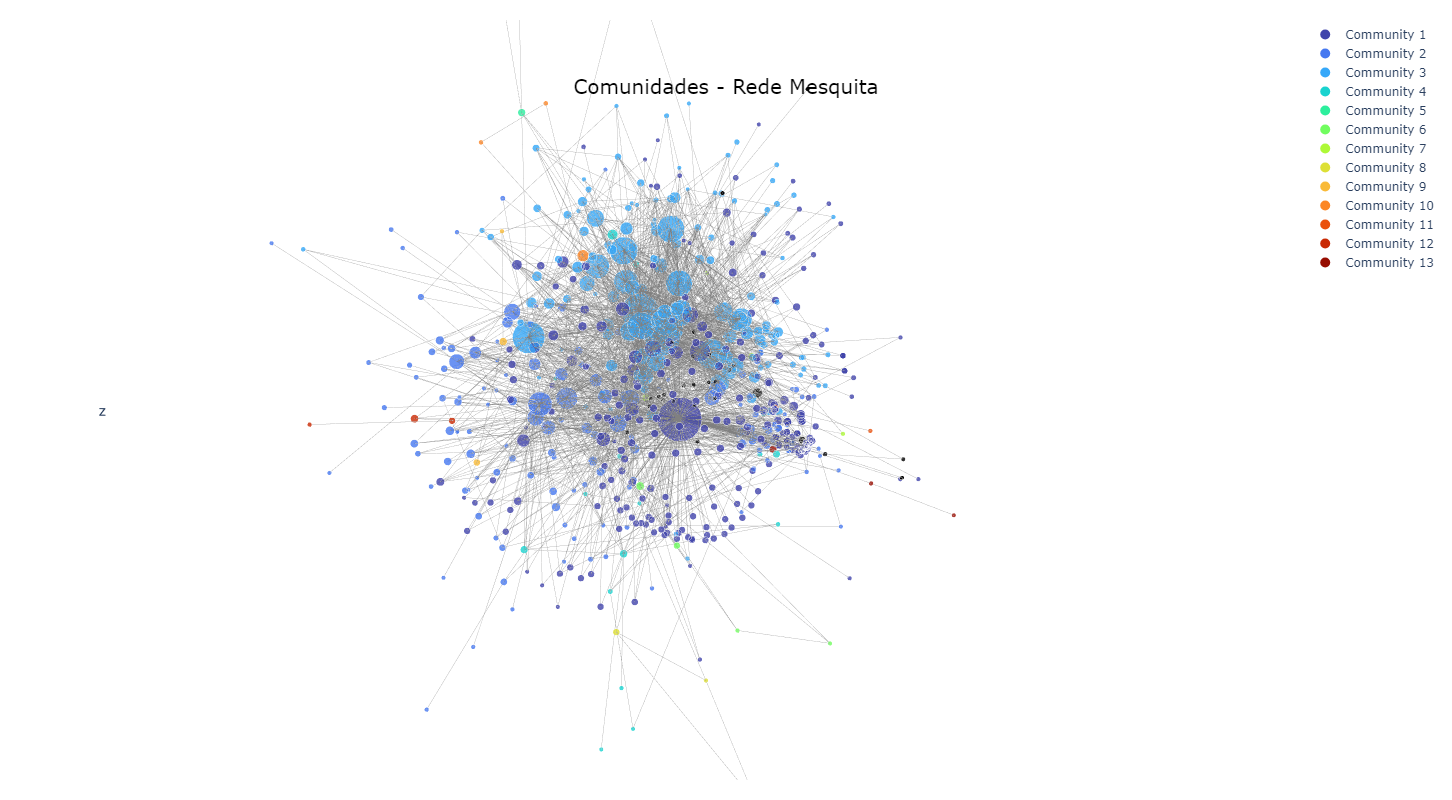
\includegraphics[scale=0.3]{images/3d_plot_example.png}
\caption{Exemplo de visualização da rede em 3D utilizando a classe \texttt{NetworkPlotter3D}. A densidade da rede pode causar o fenomeno de hairball, dificultando a interpretação.}
\label{fig:3d_plot_example}
\fautor
\end{figure}

Ao trabalhar com redes de grande escala, um obstáculo recorrente é o fenômeno denominado "hairball" (bola de pelo) \cite{2016_Tang}. Esse fenômeno manifesta-se quando a densidade de nós e arestas é tão elevada que a visualização resulta em uma aglomeração confusa, comprometendo a clareza e a interpretação. Embora o layout Kamada-Kawai apresente diversas qualidades, ele pode intensificar esse desafio em redes extensas. Isso acontece porque esse layout visa reduzir os comprimentos das arestas, o que pode ocasionar uma sobreposição indesejada de nós e arestas.

Para abordar esse desafio, introduzimos uma função de layout personalizada. Esta função utiliza heurísticas específicas para posicionar os nós de maneira que os membros da mesma comunidade sejam agrupados mais próximos, com base na influência (eigencentrality) de cada nó dentro de sua comunidade. Ao fazer isso, conseguimos uma separação clara entre diferentes comunidades, tornando-as mais notáveis e reduzindo o efeito "hairball". Esta abordagem personalizada destaca a importância de adaptar as técnicas de visualização às características específicas da rede em estudo, garantindo representações claras e informativas.

\begin{figure}[h]
	\centering
	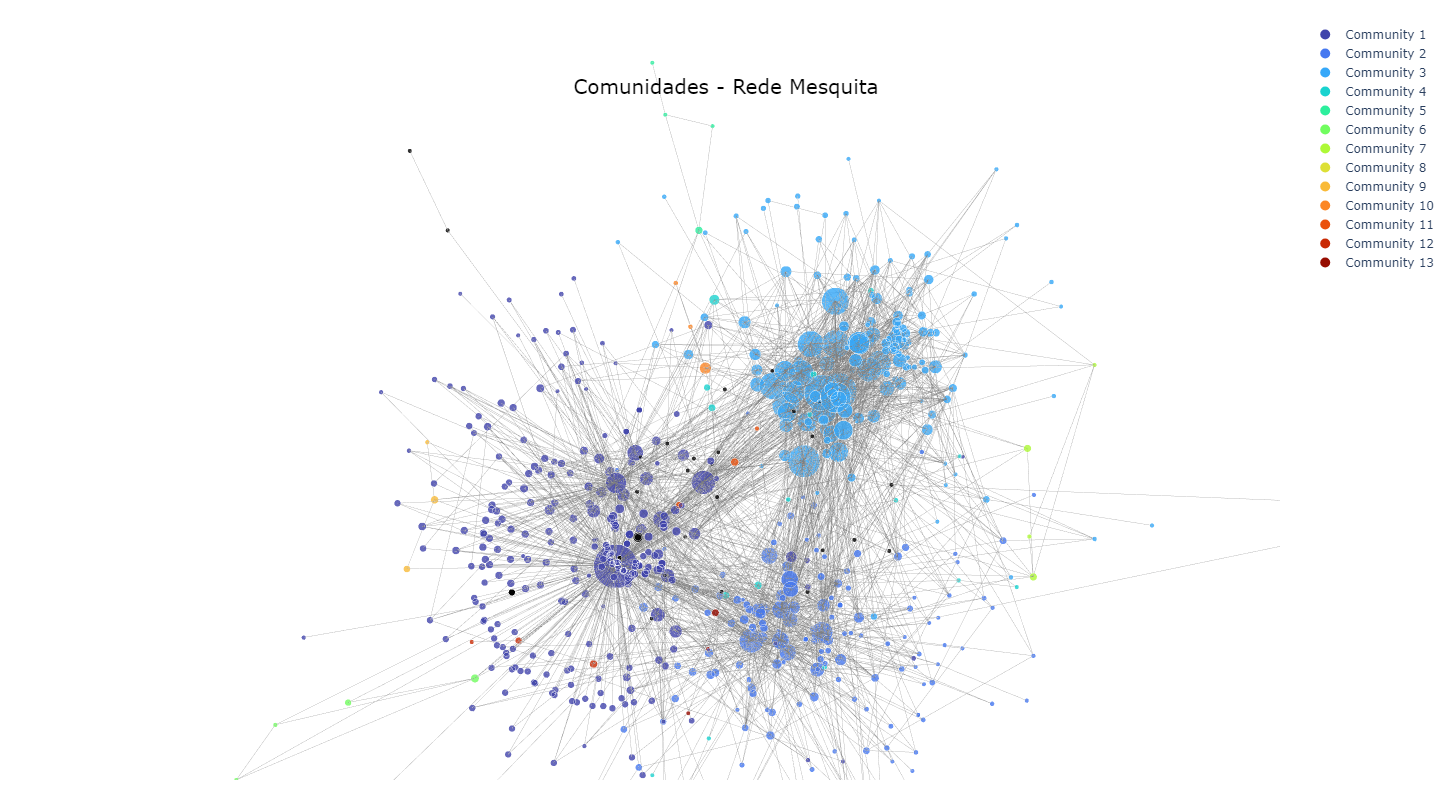
\includegraphics[scale=0.3]{images/3d_plot_hairball_buster.png}
	\caption{Exemplo de visualização da rede em 3D utilizando técnicas de layout personalizadas para reduzir o fenômeno de hairball.}
	\label{fig:3d_plot_hairball_buster}
	\fautor
\end{figure}

\section{Resultados e Discussão}

A análise exploratória de redes é uma ferramenta poderosa que nos permite desvendar as complexidades das interações sociais e compreender as dinâmicas subjacentes. Ao explorar a rede do Colab, descobrimos padrões de conexão, centralidade e comunidades que nos forneceram insights valiosos sobre o comportamento dos usuários. Esta abordagem não apenas nos permitiu visualizar a estrutura da rede, mas também identificar os usuários mais influentes e as comunidades mais ativas. Perecebe-se que o valor agregado é uma compreensão mais profunda das interações dos usuários, permitindo-nos tomar decisões informadas sobre os padrões da rede e heurísticas para detecção de câmaras de eco.

A teoria dos grafos foi nossa bússola nessa jornada exploratória. Ela forneceu o vocabulário e as técnicas necessárias e nos guiou através dos meandros da rede, ajudando-nos a identificar os caminhos mais influentes e a entender as implicações das diferentes métricas de centralidade. Através desta teoria, fomos capazes de quantificar a importância relativa dos nós e entender a estrutura global da rede. Também foi notável durante a pesquisa sobre as aplicações da teoria em análise de redes sociais, a tendência de granularizar grandes populações em subgrupos menores, permitindo uma análise mais detalhada e a identificação de padrões de interação mais sutis, tendo na rede completa uma baseline para comparação.

Nesse sentido, a topologia da rede do Colab é uma tapeçaria rica e diversificada de conexões e nós. A tabela de topologia nos oferece uma visão panorâmica da rede, permitindo-nos identificar características-chave, como a densidade da rede, o grau médio e a distribuição do grau. Estas métricas nos dão uma visão clara de como os usuários interagem e se conectam uns com os outros.

Durante nossa análise uma das primeiras observações que chamou atenção foi um alto número de cliques, que são agrupamentos de usuários altamente interconectados, indicando áreas de interação intensa e, possivelmente, a formação de comunidades centradas em tópicos específicos. Este fenômeno, característico de redes sociais dinâmicas, sugere a existência de subgrupos altamente engajados na plataforma. Paralelamente, ao avaliar as tendências de interação ao longo do tempo, conforme explorado em \autoref{sec:engajamento}, notamos um aumento nas curtidas e comentários, enquanto as conexões e avaliações de comentários apresentam uma tendência decrescente. Este padrão pode indicar uma evolução na forma como os usuários interagem, talvez focando mais em discussões em grupo do que em estabelecer novas conexões. Na teoria dos grafos, isso pode ser interpretado como uma evolução na estrutura da rede, onde os nós tendem a formar agrupamentos mais densos, potencialmente facilitando a formação de câmaras de eco. Esta observação nos sugere que, enquanto a plataforma está fomentando discussões engajadas, pode ser benéfico implementar estratégias para encorajar a formação de novas conexões, evitando assim a estagnação da rede e promovendo uma diversidade de interações. A análise de tais padrões complexos e dinâmicos é vital para entender a saúde e o crescimento sustentável da rede social, e abre avenidas para a exploração de estratégias de engajamento mais nuanceadas e eficazes.

Seguindo a estratégia de granularidade, o próximo passo foi separar a rede em comunidades, utilizamos algoritmos de detecção de comunidades, como o algoritmo de Louvain. Esses algoritmos nos permitiram identificar subgrupos dentro da rede que compartilham interesses ou características comuns, proporcionando uma visão mais granular da rede. Ao analisarmos as métricas resultantes desse processo, uma série de insights significativos emergem, contribuindo para nossa compreensão das dinâmicas das comunidades avaliadas.

Em primeiro lugar, a métrica de modularidade revelou um valor de 0.520, indicando que a divisão da rede em comunidades pelo algoritmo de Louvain é altamente significativa. Isso sugere que a estrutura da rede possui subgrupos bem definidos, onde os nós internos compartilham conexões mais densas do que com nós externos às suas respectivas comunidades. Esse nível de modularidade é fundamental para a identificação das câmaras de eco, uma vez que tais grupos tendem a ser caracterizados por uma alta coesão interna.

A distribuição dos nós por classes de modularidade é igualmente esclarecedora. Com 28\% dos nós pertencentes à Classe 1 e aproximadamente 17\% à Classe 2, percebemos que algumas comunidades são mais numerosas do que outras. Isso sugere que existem comunidades dominantes, que podem ter um papel relevante na amplificação de determinadas vozes ou crenças. Por outro lado, a presença de várias classes com menos de 1\% dos nós aponta para a existência de comunidades menores e mais especializadas, que podem desempenhar papéis igualmente importantes na disseminação de informações.

Outro insight notável provém da análise da centralidade dos usuários. Observamos que 21.04\% dos usuários têm um grau de entrada (in-degree) de 1, o que pode indicar uma forte presença de usuários periféricos na rede. Esses usuários com baixa centralidade podem ser elementos cruciais na disseminação de informações em câmaras de eco, uma vez que podem atuar como pontes entre comunidades ou grupos de interesse. Portanto, a análise de centralidade nos permite identificar não apenas os atores centrais, mas também aqueles que desempenham papéis de ligação essenciais. Com relação à centralidade de eigenvector, outra métrica crucial em nossa análise, observamos uma diversidade de valores que indicam diferentes níveis de influência dos nós na rede. Cerca de 10.23\% dos nós apresentam uma centralidade de eigenvector de 0.0, o que sugere que eles podem ter uma influência significativa na rede. Esses nós podem atuar como pontos de referência para a disseminação de informações, contribuindo para a formação de câmaras de eco. Além disso, os valores variados de centralidade de eigenvector, refletem a complexidade das interações na rede. A identificação desses nós com diferentes níveis de centralidade é fundamental para entender como a informação flui e como as câmaras de eco podem se formar e evoluir em diferentes partes da rede. Essa análise de centralidade de eigenvector complementa nossa compreensão das dinâmicas da rede, fornecendo informações adicionais sobre os atores-chave que desempenham papéis significativos na formação das câmaras de eco.

\begin{figure}[h]
    \centering
    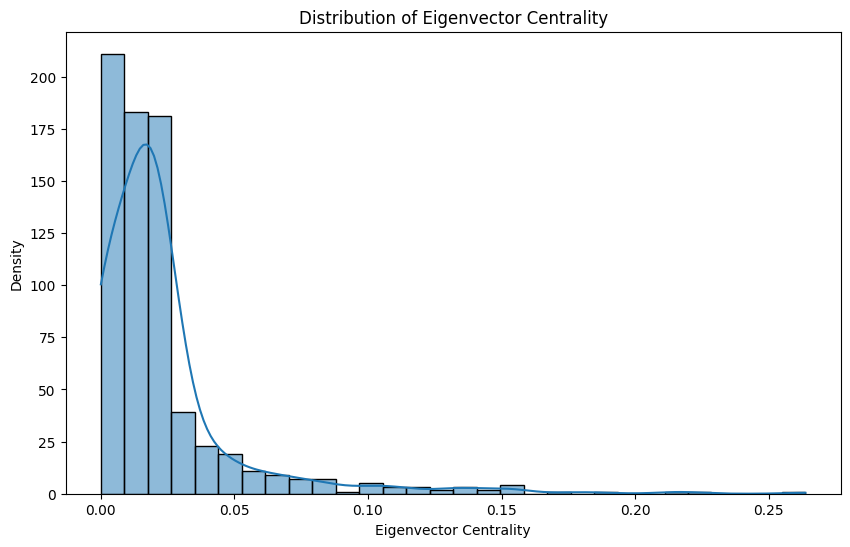
\includegraphics[scale=0.6]{images/eigencentrality.png}
    \caption{Distribuição da centralidade de eigenvector dos nós da rede.}
    \label{fig:eigencentrality}
	\fautor
\end{figure}

Analisando a demografia dos usuários, identificamos uma distribuição de gênero que favorece ligeiramente o sexo masculino, com 58.41\%, em comparação com 40.64\% de mulheres. Isso pode ter implicações na formação de câmaras de eco, uma vez que a composição demográfica influencia a dinâmica da comunicação e das crenças. Além disso, a predominância de usuários com formação de superior (54.3\%) sugere que essa rede pode estar focada em debates acadêmicos ou tópicos de maior complexidade. Essa informação é vital para entender o contexto das câmaras de eco, pois a educação desempenha um papel significativo na formação de opiniões e crenças.

A análise de idade revela uma distribuição diversificada, com nenhum grupo etário representando uma proporção dominante. Isso sugere que a rede é composta por indivíduos de diferentes faixas etárias, o que pode contribuir para a diversidade de opiniões e perspectivas. Essa heterogeneidade demográfica é relevante para a detecção de câmaras de eco, uma vez que grupos de diferentes idades podem ter abordagens distintas em relação a determinados tópicos.

A análise da excentricidade (eccentricity) da rede oferece informações sobre como os nós estão distribuídos em termos de sua distância em relação aos outros nós. Notamos que a maioria dos nós (38.25\%) possui uma excentricidade de 0, indicando que eles estão no centro da rede e, portanto, podem desempenhar papéis centrais na disseminação de informações. Por outro lado, 19.33\% dos nós têm uma excentricidade de 10, o que pode indicar a presença de nós periféricos que estão mais distantes dos demais. Essa análise da excentricidade nos permite identificar como a informação pode fluir na rede, destacando tanto os atores centrais quanto os periféricos que podem influenciar a formação de câmaras de eco.

Em resumo, a análise quantitativa dos dados resultantes da detecção de comunidades por meio do algoritmo de Louvain oferece insights cruciais para nossa compreensão das dinâmicas das câmaras de eco e das comunidades avaliadas. A modularidade da rede, a distribuição demográfica dos usuários, a centralidade dos atores e a análise de excentricidade são aspectos essenciais que nos permitem identificar padrões de interação e influência. Essas descobertas são fundamentais para entender como as câmaras de eco podem se formar e operar dentro desta rede, bem como para desenvolver estratégias eficazes de intervenção e mitigação quando necessário.

Ao focar nas três cidades com mais interações - Niterói, Santo André e Mesquita - pudemos obter uma visão mais detalhada das dinâmicas locais. Esta abordagem nos permitiu comparar e contrastar as redes destas cidades e entender as nuances regionais. A comparação da topologia das redes destas três cidades é fascinante. Mesquita, por exemplo, tem um usuário central com muitas conexões, enquanto Santo André tem vários núcleos descentralizados. Niterói, por sua vez, tem uma rede densa e integrada, indicando uma comunidade altamente interconectada. As comunidades em cada uma destas cidades também são distintas. Em Mesquita e Santo André, vemos distribuições semelhantes de comunidades, enquanto Niterói tem um cluster específico que se destaca. Estas diferenças refletem as características únicas e os padrões de interação de cada cidade.

Com as comunidades já classificadas, abre-se uma porta para a exploração mais profunda da detecção de câmaras de eco. Essas comunidades representam agrupamentos naturais de usuários em uma rede social, definidos por uma maior densidade de conexões entre seus membros. No entanto, é crucial reconhecer que nem todas as comunidades são câmaras de eco. A distinção entre esses dois conceitos é essencial para a pesquisa em questão, pois visa estabelecer critérios claros e heurísticas para a identificação precisa das câmaras de eco dentro das comunidades.

A metodologia proposta por \citeonline{2023_Atiqi_BOOK}, juntamente com a modelagem baseada em agentes, surge como uma abordagem promissora nesse contexto. Ao considerar cada usuário como um agente e simular suas interações dentro das comunidades previamente identificadas, é possível explorar como as opiniões são moldadas, reforçadas ou até mesmo silenciadas dentro desses grupos. A modelagem baseada em agentes permite analisar dinamicamente como os comportamentos individuais se traduzem em padrões coletivos de comportamento e opinião, tornando-se uma ferramenta valiosa para identificar grupos que compartilham opiniões semelhantes.

No entanto, este processo apresenta desafios significativos. Primeiramente, é preciso diferenciar comunidades normais de câmaras de eco. A simples existência de uma comunidade coesa não implica necessariamente a presença de uma câmara de eco. Portanto, a definição de critérios claros para distinguir entre esses dois conceitos é uma etapa crucial no desenvolvimento da pesquisa.

Além disso, a modelagem baseada em agentes é uma abordagem complexa, exigindo a definição cuidadosa de regras e parâmetros que governam as interações dos agentes. A dinâmica temporal das redes sociais também precisa ser considerada, uma vez que as opiniões podem evoluir ao longo do tempo, o que requer uma modelagem dinâmica.

A detecção eficaz de câmaras de eco após a identificação de comunidades requer uma análise profunda do conteúdo compartilhado e das interações entre os usuários. A análise de conteúdo pode revelar padrões de homogeneidade nas opiniões e na disseminação de informações. No \autoref{chapter:07_sentiment} abordamos a análise e a classificação do conteúdo dos usuários. Essas métricas serão usadas como insumos para as heuristicas desenvolvidas a partir da simulação de interações entre agentes, com o intuito de destacar como as opiniões podem se polarizar ou se fortalecer dentro das comunidades.

Em última análise, a combinação do técnicas eficazes de detecção de comunidades com a modelagem baseada em agentes oferece uma abordagem promissora para a identificação e compreensão das câmaras de eco em redes sociais. No entanto, é fundamental abordar os desafios mencionados e estabelecer heurísticas confiáveis para diferenciar eficazmente as câmaras de eco das comunidades tradicionais, contribuindo assim para uma compreensão mais profunda da dinâmica das redes sociais contemporâneas.

Além dos insights mencionados, é importante destacar a diversidade da rede Colab. A plataforma é um reflexo da sociedade, com usuários de diferentes idades, gêneros, etnias e níveis de educação. No entanto, observamos uma predominância de usuários masculinos, brancos e com ensino superior completo. Esta observação nos leva a refletir sobre a inclusão e representatividade na plataforma.

Olhando para o futuro, produzimos grafos no Gephi que podem ser exportados para CSV e utilizados em algoritmos em Python. Estes artefatos complementam nossa abordagem programática, permitindo-nos combinar análise visual com análise computacional.

Em conclusão, a análise da rede social do Colab nos proporcionou uma compreensão profunda das interações e dinâmicas dos usuários. Estes insights são cruciais para informar decisões estratégicas, melhorar a plataforma e promover uma comunicação mais eficaz com os cidadãos. Além disso, a metodologia desenvolvida pode ser aplicada a outras redes sociais, permitindo uma compreensão mais profunda das dinâmicas das redes sociais contemporâneas.

\chapter{Análise de sentimento das postagens do Colab}
\label{chapter:07_sentiment}
A análise de sentimento é uma técnica de processamento de linguagem natural que envolve a identificação e extração de informações subjetivas a partir de dados textuais. Esse processo pode ser usado para identificar a polaridade, ou tom emocional, de um determinado texto, o que pode ser útil em várias aplicações, como pesquisa de mercado e análise de mídias sociais \cite{2008_Pang}. Pesquisas anteriores demonstraram a utilidade da análise de sentimento em diversos domínios, incluindo política, negócios e saúde \cite{2016_Chen_IP}.

Técnicas de aprendizado de máquina podem ser usadas para automatizar o processo de análise de sentimento. Essas técnicas envolvem o treinamento de um modelo de aprendizado de máquina em um conjunto de dados rotulados, onde os rótulos indicam a polaridade dos dados textuais. Uma vez treinado, o modelo pode ser usado para prever a polaridade de novos dados textuais que não foram vistos anteriormente. Algoritmos de aprendizado de máquina comumente usados para análise de sentimento incluem regressão logística, máquinas de vetor de suporte e redes neurais \cite{2013_Haddi}.

Neste capítulo, abordamos a análise de sentimento como uma ferramenta poderosa no contexto do processamento de linguagem natural, focando especialmente nas postagens do Colab. Exploramos como técnicas de aprendizado de máquina, particularmente com o uso do Natural Language Toolkit (NLTK), podem ser empregadas para automatizar e aprimorar a análise de sentimentos. Além disso, discutimos a relevância de identificar diferentes "personas" de usuários, como os \textit{helpers} e \textit{complainers}, e como essa distinção pode influenciar a dinâmica e a polarização dentro de uma plataforma de mídia social. Finalmente, abordamos a relação entre análise de sentimento, polarização e a formação de câmaras de eco, destacando a importância de entender e mitigar esses fenômenos em ambientes digitais.

\section{Processamento de linguagem natural e Análise de sentimento}

A análise de sentimento, um pilar do processamento de linguagem natural (PLN), é fundamental para decifrar o conteúdo emocional e as opiniões expressas em textos. Ao aplicar essa técnica em contextos variados, de estudos de mercado a análises de redes sociais, pesquisadores podem extrair tendências e padrões valiosos a partir de dados textuais \cite{2008_Pang, 2015_Nguyen}.

Em nosso estudo, exploramos a capacidade do Natural Language Toolkit (NLTK), uma biblioteca de PLN para Python, para conduzir uma análise de sentimento automatizada. O NLTK disponibiliza ferramentas como classificadores, léxicos e algoritmos de processamento de texto \cite{2009_Bird_BOOK}. O dicionário léxico VADER, parte do NLTK, é projetado para captar nuances em textos de mídias sociais, incluindo gírias e emojis \cite{2014_Hutto}.

Contudo, o VADER e outros recursos do NLTK têm um enfoque no inglês, o que apresenta um obstáculo quando aplicado a idiomas distintos. Diante da predominância do português em nosso conjunto de dados, recorremos ao LeIA, um léxico adaptado ao português brasileiro, para uma avaliação mais acurada dos sentimentos \cite{2018_Almeida_PAGE}. A combinação do NLTK com o LeIA permitiu uma análise mais refinada, considerando as particularidades do português no conteúdo do Colab.

O processo de análise começa com o pré-processamento dos textos, que inclui tokenização e a remoção de palavras irrelevantes. Cada token é então avaliado segundo o léxico para determinar sua polaridade e, por fim, estabelecer uma pontuação geral para o texto \cite{2013_Haddi}. O uso de técnicas avançadas de PLN, incluindo lematização e algoritmos de aprendizado de máquina como regressão logística e redes neurais, aumenta a precisão da análise \cite{2014_Kim}.

Na plataforma Colab, a análise de sentimento é empregada para identificar padrões de homofilia e polarização. Estudos têm mostrado a viabilidade dessa técnica para inferir posicionamentos políticos e emocionais dos usuários nas mídias sociais \cite{2014_Hutto}. A homofilia, que descreve a tendência de interação entre usuários com opiniões e sentimentos semelhantes, é um indicador de polarização e pode ser mensurada através da análise de sentimento. Esta análise fornece uma métrica quantitativa da polarização e dos temas que catalisam a formação de câmaras de eco.

Considerando a importância da opinião pública em diversos aspectos da sociedade, incorporamos no modelo de dados do Colab métricas de 'score' e 'persona' baseadas nos sentimentos das postagens. O 'score' reflete a valência do sentimento das postagens, enquanto a 'persona' encapsula a tendência comportamental dos usuários. Essas métricas, somadas às ferramentas de PLN adaptadas ao português, permitem uma análise de sentimento contextualizada e relevante para a plataforma \cite{2012_Souza_IP}.

\subsection*{Análise de Sentimento, Homofilia e Polarização}

A análise de sentimento nas redes sociais não apenas ilumina o humor e a opinião dos usuários, mas também serve como uma lente para examinar a homofilia e a polarização dentro dessas comunidades digitais. Homofilia, a propensão para a associação e interação com indivíduos de características similares, pode ser quantificada por meio da análise de sentimento das postagens dos usuários. Por exemplo, usuários cujas postagens e interações são predominantemente positivas tendem a formar subgrupos de homofilia positiva, enquanto aqueles com interações e postagens negativas tendem a se agrupar, potencialmente levando a um aumento da polarização.

Esta tendência é particularmente relevante na detecção de câmaras de eco, onde a homofilia pode se manifestar não apenas em opiniões compartilhadas, mas também no sentimento coletivo. Uma análise detalhada do sentimento expresso nas postagens pode revelar a inclinação emocional de um grupo e, consequentemente, medir sua polarização. Um alto grau de homofilia em sentimento, seja positivo ou negativo, pode indicar a presença de uma câmara de eco, caracterizada pela repetição e reforço de um ponto de vista homogêneo.

Além disso, a análise de sentimento oferece uma maneira de desvendar os temas subjacentes que fomentam a polarização. Ao discernir os sentimentos associados a tópicos específicos, podemos entender quais questões estão no coração das câmaras de eco e como elas influenciam a dinâmica do grupo. Tais insights são cruciais para desenhar estratégias eficazes que promovam o diálogo e a diversidade de pensamento dentro das redes sociais.

A pesquisa de \citeonline{2014_Colleoni}, por exemplo, destaca a aplicabilidade da análise de sentimento na medição da polarização política no Twitter. Evidenciou-se que os usuários são atraídos para comunidades de sentimento similar, o que pode levar à formação de câmaras de eco. A análise de sentimento emergiu, assim, como uma ferramenta estratégica para identificar influenciadores-chave da polarização, possibilitando intervir com perspectivas alternativas e fomentar um espaço mais equilibrado para o discurso público.

No Colab, a Análise de Sentimento é empregada para medir essa homofilia e avaliar a polarização das discussões. Utilizando métricas derivadas da valência dos sentimentos expressos nas postagens, é possível quantificar até que ponto grupos de usuários compartilham uma visão unilateral, potencialmente cedendo à polarização. Essas métricas são vitais para identificar os tópicos que polarizam as conversas e as 'personas' que podem estar contribuindo para esse fenômeno.

A polarização é um indicador significativo do risco de formação de câmaras de eco. Quando um grupo de usuários apresenta predominantemente sentimentos semelhantes em suas postagens, isso sugere uma maior probabilidade de que eles estejam reforçando as crenças um do outro sem a exposição a pontos de vista alternativos. A identificação desses padrões pode ser crucial para o desenvolvimento de intervenções destinadas a promover um ambiente de debate mais balanceado e menos polarizado.

No Colab, a Análise de Sentimento é empregada para medir essa homofilia e avaliar a polarização das discussões. Utilizando métricas derivadas da valência dos sentimentos expressos nas postagens, é possível quantificar até que ponto grupos de usuários compartilham uma visão unilateral, potencialmente cedendo à polarização. Essas métricas são vitais para identificar os tópicos que polarizam as conversas e as 'personas' que podem estar contribuindo para esse fenômeno.

A polarização é um indicador significativo do risco de formação de câmaras de eco. Quando um grupo de usuários apresenta predominantemente sentimentos semelhantes em suas postagens, isso sugere uma maior probabilidade de que eles estejam reforçando as crenças um do outro sem a exposição a pontos de vista alternativos. A identificação desses padrões pode ser crucial para o desenvolvimento de intervenções destinadas a promover um ambiente de debate mais balanceado e menos polarizado.

Ademais, a análise de sentimento oferece insights sobre os conteúdos específicos que estão impulsionando a polarização. Investigando as postagens e os temas mais discutidos, podemos compreender os fatores que contribuem para a manutenção das câmaras de eco. Isso não apenas esclarece a natureza da polarização na rede, mas também fornece um caminho para estratégias que possam facilitar um diálogo mais diverso e inclusivo.

Por fim, o estudo das interações no Colab, com a ajuda da análise de sentimento, destaca a importância de entender as dinâmicas de homofilia e polarização e sua influência na formação de opiniões. Ao incorporar essa compreensão em nossas métricas analíticas, podemos começar a desenhar uma estratégia mais eficaz para combater a polarização e promover um diálogo mais rico e variado, essencial para o bem-estar de qualquer comunidade online.

\section{Análise exploratória de Sentimento}

Neste capítulo, nos aprofundamos na análise de sentimentos das postagens do Colab, introduzindo a métrica de "score". Esta métrica foi desenvolvida especificamente para este estudo, com o intuito de classificar as postagens como positivas ou negativas, proporcionando uma visão mais quantitativa dos sentimentos expressos pelos usuários. Além disso, apresentamos uma análise exploratória dos dados, com o objetivo de identificar os principais tópicos discutidos no Colab e as principais palavras associadas a cada tópico. Por fim, adicionamos uma camada de análise de redes no experimento, introduzindo a assortatividade como uma métrica para medir a homofilia na rede.

Para realizar essa análise, fundamentamos nosso estudo em conceitos e técnicas de processamento de linguagem natural (PLN) e análise de sentimentwos. O PLN é uma área da inteligência artificial que visa capacitar os computadores a entender, interpretar e gerar linguagem humana de forma natural. A análise de sentimentos, por sua vez, é uma subárea do PLN que se concentra em identificar e extrair informações sobre os sentimentos e opiniões expressos em textos.

Utilizamos a linguagem de programação Python como base para a implementação do experimento. Como runtime, novamente utilizamos o Google Colab, que nos permite executar o código em nuvem, sem a necessidade de instalar bibliotecas ou configurar o ambiente de desenvolvimento. O código-fonte do experimento está disponível no GitHub\footnote{https://github.com/guinetik/colab-network-ec}.

Com a aplicação dessas técnicas e o uso da linguagem Python, pudemos extrair insights valiosos sobre os sentimentos presentes nas postagens do Colab. Essas métricas servirão como base para as análises subsequentes e contribuirão para aprimorar a compreensão do ecossistema do Colab.

\subsection{Heurísticas para classificação de postagens por score de sentimento}

No capítulo anterior, realizamos uma análise exploratória da rede, identificando comunidades de usuários e suas interações. Neste contexto, a classificação de postagens por score torna-se uma ferramenta valiosa. Esta métrica categoriza as postagens como positivas, negativas ou neutras com base em seu conteúdo textual, utilizando uma abordagem de pontuação de sentimentos. Cada postagem recebe um score de sentimento que varia de -1 (negativo) a 1 (positivo), com scores próximos a 0 indicando neutralidade. Esta abordagem quantitativa não só nos permite capturar o sentimento geral expresso nas postagens, mas também entender como esses sentimentos se propagam e interagem dentro da rede. Assim, podemos obter insights valiosos sobre a percepção dos usuários em relação a diferentes tópicos e como essa percepção influencia a estrutura e a dinâmica da rede.

Para uma análise mais aprofundada, é crucial preparar adequadamente os dados para a classificação supervisionada de sentimentos. Utilizamos técnicas avançadas de Processamento de Linguagem Natural (PLN) para analisar postagens do Colab. O objetivo é classificar as postagens de forma eficaz, com base em seu conteúdo textual. Para isso, empregamos a biblioteca Spacy para tarefas de PLN e a biblioteca NLTK para tokenização e lematização. Além disso, as bibliotecas pandas e matplotlib são utilizadas para manipulação e visualização de dados, respectivamente. Esta preparação meticulosa dos dados é fundamental para treinar um algoritmo de classificação robusto e preciso. Os próximos parágrafos exploram as heurísticas e técnicas utilizadas para esse modelo de classificação.

\begin{figure}[!htb]
	\caption{Demonstração do mapa sintático de uma frase utilizando o pacote Stanza para NLP, Deplacy para grafo de dependências e matplotlib para renderização.}
	\label{fig:lexicon_breakdown}
	\centering
	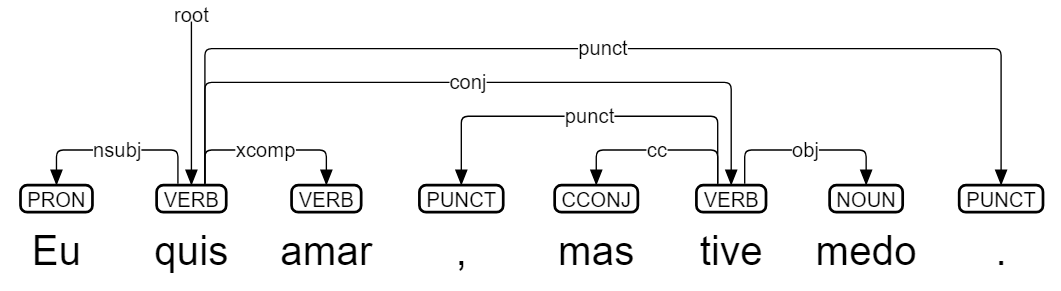
\includegraphics[scale=0.5]{images/lexicon_breakdown.png}
	\fautor
\end{figure}

A Análise de sentimentos emprega várias técnicas de \sigla{PLN}{Processamento de Linguagem Natural}, incluindo tokenização, lematização e remoção de palavras irrelevantes ou stop-words. A tokenização consiste em dividir o texto em palavras individuais ou "tokens". Já a lematização visa reduzir as palavras à sua forma base ou raiz, o que ajuda a consolidar diferentes formas da mesma palavra. Por sua vez, a remoção de palavras irrelevantes envolve a eliminação de termos comuns que geralmente não contribuem para o significado de uma frase, como "e", "o" e "em".Além dessas técnicas, a análise de sentimentos também se beneficia do uso de dicionários léxicos pré-existentes. Esses dicionários são valiosos recursos que contêm palavras associadas a valores de polaridade, indicando o sentimento geral de cada termo (positivo, negativo ou neutro).

No contexto da análise de sentimentos, existem vários dicionários léxicos relevantes disponíveis. Esse estudo comparou quatro repositórios bastante populares:

\begin{itemize}
	\item OpLexicon \cite{2011_Souza_IP}: É um dicionário léxico específico para o idioma português, com mais de 32.000 palavras, cada uma acompanhada de um valor de polaridade associado.
	\item SenticNet \cite{2016_Cambria_IP}: É dicionário léxico multilíngue que fornece valores de polaridade para palavras com base em sua semântica e psicologia.
	\item UniLex: Outro dicionário léxico multilíngue que oferece valores de polaridade para palavras com base em uma variedade de recursos linguísticos.
	\item WordNetAffectBR \cite{2008_Pasqualotti}: Esta é uma versão em português do WordNet-Affect, um dicionário léxico que atribui valores de polaridade às palavras com base em sua associação com diferentes emoções.
\end{itemize}

Ao utilizar esses dicionários léxicos, podemos comparar as palavras presentes no texto com as entradas nos dicionários para determinar a polaridade de cada uma. Isso nos possibilita obter uma compreensão mais abrangente dos sentimentos expressos no texto, contribuindo para uma análise de sentimentos mais precisa e eficaz. Esses dicionários são ferramentas valiosas no campo da análise de sentimentos, auxiliando na identificação e interpretação das emoções presentes nas palavras utilizadas. Além disso, com base nesses recursos, é possível automatizar e ampliar a análise de sentimentos em textos extensos, como avaliações de produtos, publicações em redes sociais e outros tipos de conteúdo textual.

Durante a comparação da polaridade da frase de teste com os dicionários léxicos, notou-se uma discrepância na normalização dos dicionários Unilex e WordNetAffectBR. Para este experimento, optamos por utilizar apenas o OpLexicon e o SenticNet, devido aos seus scores similares de polaridade e à presença de palavras exclusivas em cada um desses dicionários.

Além disso, realizamos um teste utilizando um \textit{subset} dos dados das postagens do Colab para adequação ao contexto. Durante esse teste, identificamos palavras relevantes que não estavam presentes nos dicionários léxicos originais. Adicionamos manualmente essas palavras ao conjunto de dicionários, atribuindo-lhes scores de -1 a 1 com base na polaridade observada nas postagens do Colab.

Em seguida, realizamos uma análise comparativa para avaliar a eficácia desses dicionários léxicos. Durante essa análise, calculamos a polaridade resultante para cada um dos dicionários, buscando identificar qual deles é mais eficaz na análise de sentimentos no contexto específico das postagens do Colab. Como resultado, obtivemos um amalgama dos dicionários OpLexicon e SenticNet, além do conjunto de palavras que foram adicionadas manualmente. Essas palavras foram normalizadas e incorporadas ao processo de análise.

O processo de análise de sentimento das postagens começa com o carregamento dos dados. Nessa análise, estamos interessados em postagens criadas por usuários das comunidades identificadas na análise do capítulo anterior, nas cidades de Niterói, Santo André e Mesquita. Em seguida, realizamos o pré-processamento do texto, que envolve a remoção de caracteres especiais, conversão para letras minúsculas, tokenização e aplicação de técnicas de stemização para reduzir as palavras às suas formas básicas \cite[]{2009_Bird_BOOK}.

Utilizamos a técnica de "bag-of-words" descrita em \citeonline{2013_Mikolov} com a biblioteca CountVectorizer para converter o texto em uma matriz numérica, onde cada coluna representa uma palavra e cada linha representa uma postagem. Com base nessa matriz, identificamos as palavras mais frequentes e as visualizamos em um gráfico de barras e na forma de uma nuvem de palavras.

\begin{figure}[!htb]
	\caption{Distribuição de palavras mais frequentes}
	\label{fig:wordcount}
	\centering
	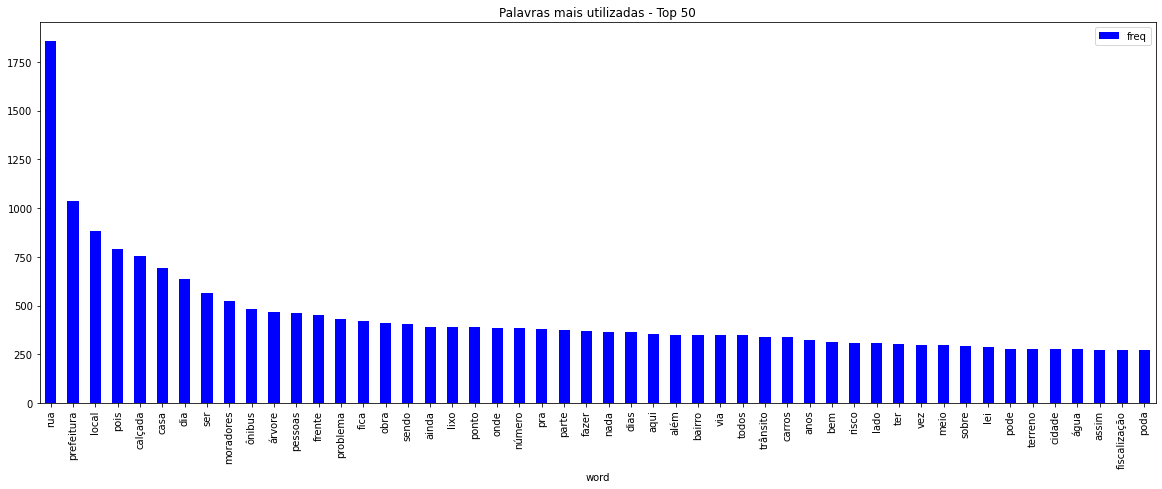
\includegraphics[scale=0.35]{images/wordcount.png}
	\fautor
\end{figure}

Realizamos uma análise exploratória dos dados para entender melhor as características das postagens. Isso incluiu a visualização da distribuição das palavras mais frequentes e a criação de nuvens de palavras para postagens positivas e negativas. Além disso, utilizamos a biblioteca Word2Vec para criar um modelo de palavras em vetores, que foi usado para visualizar as associações de palavras mais comuns.

\begin{figure}[!htb]
	\caption{Núvem de palavras mais utilizadas}
	\label{fig:wordcloud}
	\centering
	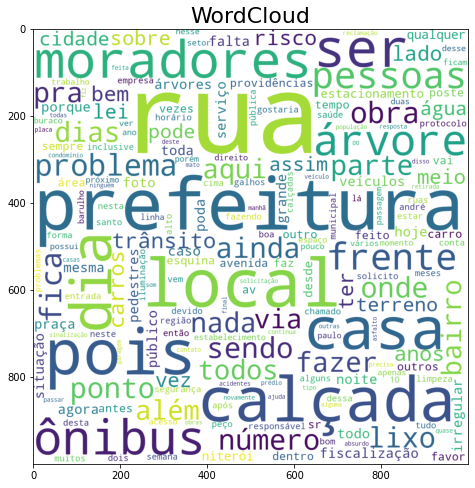
\includegraphics[scale=0.5]{images/wordcloud.png}
	\fautor
\end{figure}

\begin{figure}[htb]
	\centering
	\caption{Comparação de núvem de palavras mais usadas}\label{fig:lexicon_tagcloud}
	\begin{subfigure}[b]{0.317\textwidth}
		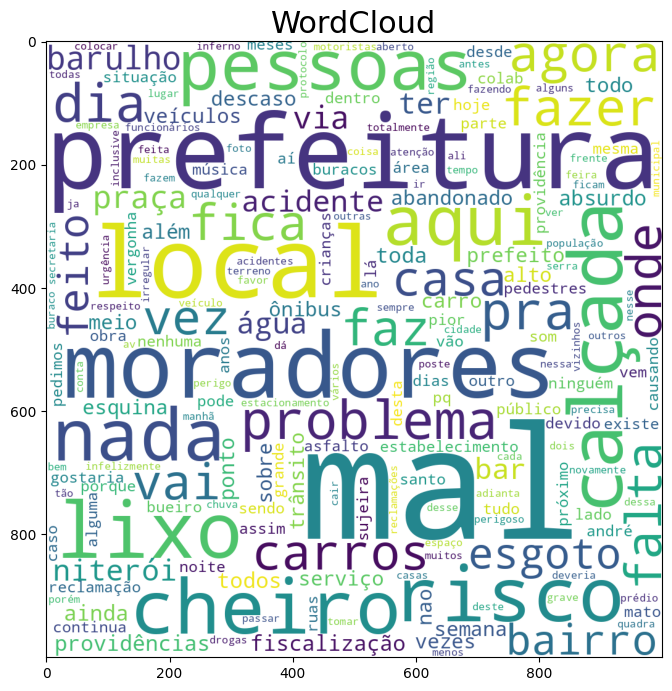
\includegraphics[width=\textwidth]{images/lexicon_worst_scores_tagcloud.png}
		\caption{Scores Negativos}
		\label{fig:tigre}
	\end{subfigure} ~ %add desired spacing between images, e. g. ~, \quad, \qquad, \hfill etc. %(or a blank line to force the subfigure onto a new line) 
	\begin{subfigure}[b]{0.317\textwidth}
		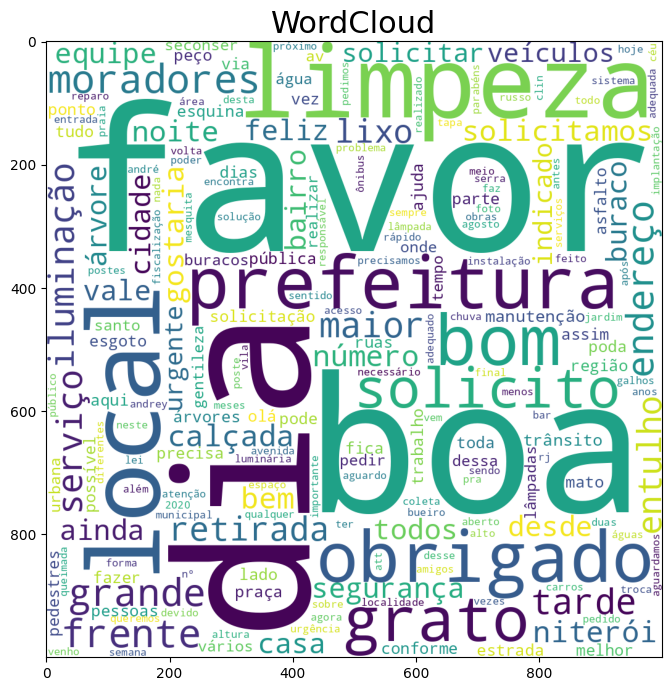
\includegraphics[width=\textwidth]{images/lexicon_best_scores_tagcloud.png}
		\caption{Scores Positivos} \label{fig:leao}
	\end{subfigure} ~ %add desired spacing between images, e. g. ~, \quad, \qquad, \hfill etc. %(or a blank line to force the subfigure onto a new line)
	\fautor
\end{figure}

Durante a análise exploratória, observamos uma tendência intrigante: muitos usuários optavam por se comunicar usando emojis. Em algumas instâncias, os emojis eram usados para complementar o texto, enquanto em outras, eles eram a principal forma de expressão. Isso levantou a questão sobre a polaridade sentimental desses emojis. Para abordar essa questão, recorremos ao dataset de sentimentos de emojis criado por \citeonline{2015_Novak}. Este conjunto de dados oferece uma classificação de sentimentos para emojis comuns, permitindo-nos incorporar essa dimensão em nossa análise.

Além dos emojis, notamos a presença de jargões específicos frequentemente usados pelos usuários do aplicativo. Estes jargões, muitas vezes, carregavam um significado ou conotação que não era imediatamente claro para quem não estava familiarizado com o contexto do aplicativo. Reconhecendo a importância desses jargões na análise de sentimentos, decidimos classificar manualmente a polaridade dos 100 jargões mais comuns encontrados no app. Isso também incluiu a identificação e classificação de nomes de partidos políticos, dada a sua relevância no discurso dos usuários.

Outro aspecto que chamou nossa atenção foi a presença de profanidades nas postagens. A linguagem ofensiva ou abusiva pode ter um impacto significativo na polaridade de uma postagem. Portanto, introduzimos uma etapa adicional em nossa análise para detectar essas profanidades. Ao identificá-las, classificamos essas palavras com uma polaridade negativa, garantindo que sua presença influenciasse adequadamente o score de sentimento da postagem em questão. Com essas etapas adicionais, buscamos uma análise de sentimentos mais robusta e contextualizada, levando em consideração as peculiaridades e nuances do discurso dos usuários no aplicativo.

Na busca por uma análise mais refinada e contextualizada dos sentimentos expressos nas postagens do Colab, decidimos incorporar uma métrica adicional ao nosso estudo: a análise de sentimentos realizada pelo pacote LeIA \cite{2018_Almeida_PAGE}. A inclusão dessa ferramenta visa aprimorar a nossa abordagem ao oferecer uma análise mais nuanceada dos sentimentos expressos nos textos, levando em consideração aspectos como a presença de emojis e a estrutura linguística das frases.

A ferramenta LeIA, desenvolvida especificamente para a língua portuguesa, apresenta uma abordagem que vai além da simples classificação de palavras individuais, oferecendo uma análise sintática e semântica mais profunda dos textos. Através da análise de sentimentos realizada pelo LeIA, obtemos uma pontuação composta (compound) que varia de -1 a +1, indicando o sentimento geral do texto, além de valores percentuais que representam a proporção de sentimentos positivos, negativos e neutros presentes no texto.

Para integrar essa métrica ao nosso estudo, adaptamos nossa função de análise de sentimentos para incluir a análise realizada pelo LeIA. Cada postagem do dataset foi analisada individualmente, gerando scores detalhados que incluem as métricas de positividade, negatividade, neutralidade e a pontuação composta. Esses scores foram então adicionados ao nosso dataset, prefixados com "leia" para indicar sua origem.

A decisão de integrar as métricas provenientes dos dicionários léxicos com as fornecidas pelo LeIA é motivada pela busca de uma análise mais holística e robusta. Enquanto nossos dicionários léxicos oferecem uma vasta base de palavras já classificadas, proporcionando uma análise ampla e generalizada, o LeIA traz uma perspectiva mais detalhada e contextual, capaz de interpretar nuances e particularidades da língua portuguesa, como a influência de emojis e a presença de negações no sentimento expresso. No entanto, é crucial reconhecer que tanto os dicionários léxicos quanto o LeIA podem introduzir seus próprios vieses na análise. Ao combinar essas métricas, aspiramos mitigar esses vieses individuais, buscando uma representação mais neutra e equilibrada dos sentimentos. A métrica composta, nesse contexto, não só permite uma categorização mais fluida dos sentimentos, evitando a rigidez das categorizações binárias, mas também proporciona uma visão mais matizada e imparcial dos dados.

Ao explorar a sinergia entre as métricas tradicionais e a análise realizada pelo LeIA, estamos em busca de respostas para uma questão central: como podemos, através da combinação de diferentes técnicas de análise de sentimentos, alcançar uma representação mais fiel e detalhada dos sentimentos expressos pelos usuários? Acreditamos que essa abordagem multidimensional pode revelar padrões e insights que seriam invisíveis através de uma única métrica. No entanto, é crucial enfatizar que a combinação de métricas apresenta desafios intrínsecos, sobretudo no que tange à calibração e à interpretação dos resultados. A integração das métricas não é uma simples concatenação de valores; ela demanda um processo meticuloso de normalização. Em nosso estudo, realizamos uma normalização dos scores para assegurar que as métricas provenientes de diferentes fontes estivessem em uma escala comum e comparável. Esse processo é fundamental para garantir que a combinação dos scores preserve a integridade e a precisão da análise, permitindo uma interpretação coesa e coerente dos sentimentos expressos nas postagens.

Para validar nossa abordagem, planejamos realizar uma série de testes e análises exploratórias, buscando entender como as métricas combinadas podem oferecer uma visão mais completa e rica dos sentimentos expressos nas postagens do Colab. Através dessa análise multidimensional, aspiramos a desvendar as complexidades do discurso dos usuários, oferecendo insights valiosos para a compreensão das dinâmicas sociais e emocionais presentes na plataforma.

Ao analisar a amostra fornecida, notamos que a combinação de métricas não apenas amplia a perspectiva sobre o sentimento, mas também ajuda a identificar nuances que poderiam ser perdidas se confiássemos em uma única métrica. Por exemplo, enquanto o score derivado dos dicionários léxicos pode capturar a polaridade geral de uma postagem, o leia\_compound do LeIA pode identificar sutilezas, como a influência de emojis ou a presença de negações, que podem alterar significativamente a interpretação do sentimento.

Além disso, observamos que a métrica composta compound\_score oferece uma visão mais equilibrada e matizada do sentimento. Em casos onde o score e o leia\_compound divergem, o compound\_score serve como uma espécie de "árbitro", proporcionando uma avaliação que leva em consideração ambas as perspectivas. Isso é particularmente útil em postagens onde o sentimento é ambíguo ou onde diferentes aspectos da postagem sugerem sentimentos contrastantes.

Outro insight interessante é a maneira como o compound\_score pode ajudar a identificar postagens que são particularmente polarizadas ou que geram sentimentos mistos. Postagens com compound\_scores próximos de zero, por exemplo, podem indicar postagens que contêm elementos tanto positivos quanto negativos, sugerindo que elas são mais complexas e merecem uma análise mais aprofundada.

Além disso, ao combinar métricas, também estamos abordando potenciais vieses inerentes a cada abordagem individual. Enquanto os dicionários léxicos podem ter suas próprias limitações e preconceitos, o LeIA, sendo uma ferramenta de aprendizado de máquina, pode ter seus próprios vieses com base nos dados com os quais foi treinado. Ao combinar essas métricas, esperamos criar uma métrica mais robusta e imparcial.

Em conclusão, ao adotar uma abordagem multidimensional para a análise de sentimentos, estamos não apenas buscando uma representação mais precisa do sentimento, mas também tentando entender as complexidades e nuances do discurso dos usuários. Esta abordagem combinada promete oferecer insights mais ricos e detalhados, permitindo uma compreensão mais profunda das emoções e opiniões expressas na plataforma Colab.

\section{Análise de sentimento nas redes de Niterói, Santo André e Mesquita}

\begin{figure}[!htb]
	\caption{Distribuição dos scores de sentimento nas postagens da rede das 3 cidades selecionadas. Cada ponto representa um usuário e a cor indica o score médio de sentimento de suas postagens (verde para positivo, vermelho para negativo e laranja para neutro)}
	\label{fig:scores_scatterplot}
	\centering
	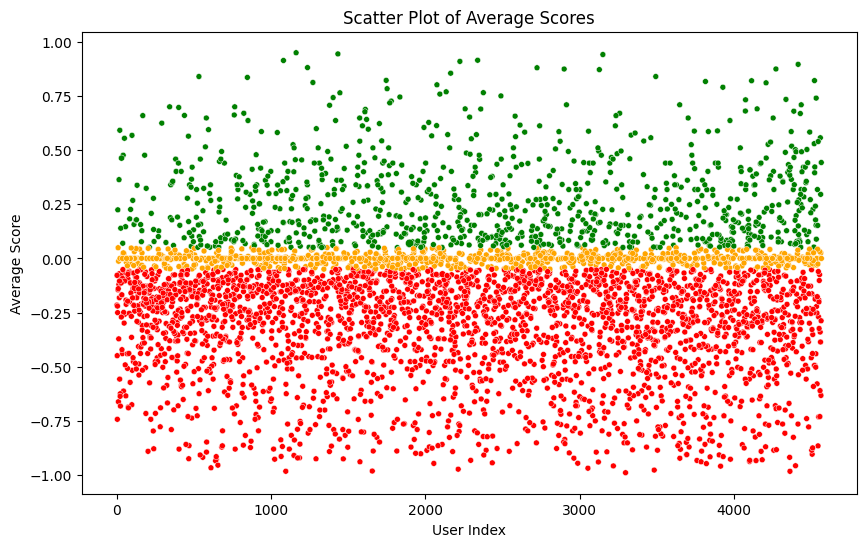
\includegraphics[scale=0.70]{images/scores_scatterplot.png}
	\fautor
\end{figure}

Após a seleção das postagens dos usuários das comunidades das cidades de Niterói, Santo André e Mesquita, conforme detalhado no capítulo anterior, foi possível identificar um total de 132.846 eventos de zeladoria criados por membros dessas comunidades. Esta vasta quantidade de dados nos ofereceu uma oportunidade única para aprofundar nossa análise de sentimentos e entender melhor as emoções e opiniões expressas pelos usuários.

Ao aplicar a análise de sentimentos nas postagens, foi essencial considerar a extensão dos textos. Uma postagem mais longa tem naturalmente mais palavras e, consequentemente, uma maior soma de polaridades. Para contornar essa característica e garantir uma análise justa, optamos por normalizar os scores com base no número de tokens ou palavras presentes na frase original. Esta abordagem permitiu que cada palavra contribuísse proporcionalmente para o score final da postagem, independentemente do seu tamanho.

Ao examinar os melhores scores, notamos algumas tendências interessantes. Primeiramente, as postagens com os scores mais elevados tendem a ter uma combinação de sentimentos neutros e positivos, conforme indicado pelas métricas do LeIA. Por exemplo, a postagem do evento 100876, originada de Niterói, apresenta uma combinação de 75,1\% de conteúdo neutro e 16,8\% de conteúdo positivo, resultando em um score composto de 0,671. Isso sugere que, mesmo quando os usuários estão apresentando informações factuais ou descritivas, há uma inclinação positiva em suas expressões.

Além disso, é notável que, mesmo com variações nos scores derivados dos dicionários léxicos, o LeIA consistentemente percebeu essas postagens como altamente positivas. Isso pode ser atribuído à capacidade do LeIA de capturar nuances e contextos específicos da língua portuguesa, como a influência de emojis e a presença de negações.

Outro ponto de destaque é a variedade de temas abordados nas postagens com os melhores scores. Enquanto algumas postagens, como a do evento 321209 de Santo André, focam em questões de zeladoria como o acúmulo de lixo, outras, como a do evento 328652, discutem colaborações entre organizações privadas e públicas. Isso reforça a ideia de que a plataforma Colab é um espaço diversificado, onde os usuários se sentem empoderados para discutir uma ampla gama de tópicos relacionados à melhoria de suas comunidades.

Em resumo, a análise dos melhores scores nos proporcionou uma visão mais clara das emoções e opiniões dos usuários nas comunidades selecionadas. Estes insights são fundamentais para entender as motivações dos usuários ao interagir na plataforma e podem ser usados para orientar futuras estratégias de engajamento e moderação.

\begin{figure}[!htb]
	\caption{Score médio de sentimento por número de usuários}
	\label{fig:average_score_by_number_of_users}
	\centering
	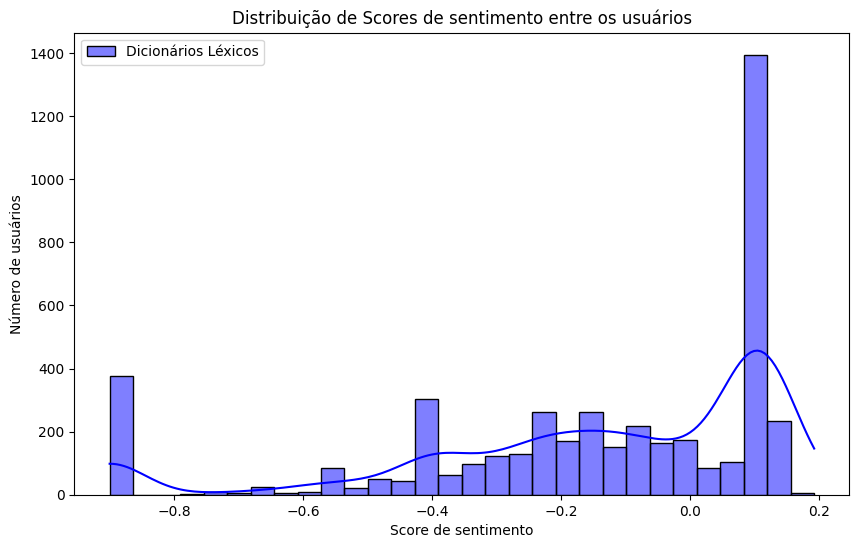
\includegraphics[scale=0.70]{images/average_score_by_number_of_users.png}
	\fautor
\end{figure}

Ao analisar os piores scores, é evidente que as postagens refletem um alto grau de insatisfação e frustração dos usuários em relação a questões específicas de zeladoria em suas comunidades. Estas postagens, oriundas das cidades de Niterói e Rio de Janeiro, destacam-se não apenas pelo conteúdo negativo, mas também pela intensidade das emoções expressas.

A postagem do evento 218258, por exemplo, menciona a repetição de reclamações feitas pelo usuário sem a devida solução, indicando um sentimento de desamparo e descontentamento com a resposta (ou falta dela) das autoridades competentes. O score derivado do dicionário léxico para esta postagem foi de -2.857, enquanto o LeIA identificou uma predominância de conteúdo neutro (73,5\%), mas com uma porcentagem significativa de conteúdo negativo (19,9\%). O score composto, que combina ambas as métricas, resultou em -0.957, refletindo a natureza altamente negativa da postagem.

Da mesma forma, a postagem do evento 156161 expressa indignação com a situação de uma rua específica, usando palavras em caixa alta para enfatizar o descontentamento. O uso de termos como "ABSURDO" e "CAOS" sugere uma forte emoção negativa. O LeIA capturou essa nuance, atribuindo um score negativo de -0.9930, enquanto o score do dicionário léxico foi de -0.167. A combinação de ambos resultou em um score composto de -0.956.

É interessante notar que, mesmo nas postagens com os piores scores, ainda há uma presença de conteúdo neutro e, em alguns casos, até mesmo positivo. Por exemplo, a postagem do evento 239454, apesar de expressar frustração com tentativas repetidas de comunicação, ainda contém uma saudação cordial ("Olá prezados"). Isso sugere que, mesmo em meio à insatisfação, os usuários ainda buscam manter um tom respeitoso e construtivo em suas comunicações.

Em resumo, as postagens com os piores scores ilustram claramente os desafios e frustrações enfrentados pelos usuários em suas comunidades. Estas postagens são valiosas, pois destacam áreas que requerem atenção imediata e melhorias por parte das autoridades locais. Além disso, a análise de sentimentos fornece uma ferramenta poderosa para identificar e compreender essas preocupações, permitindo uma resposta mais eficaz e empática por parte dos tomadores de decisão.

\begin{figure}[!htb]
	\caption{Distribuição de quantidade de postagens por score}
	\label{fig:score_distribution}
	\centering
	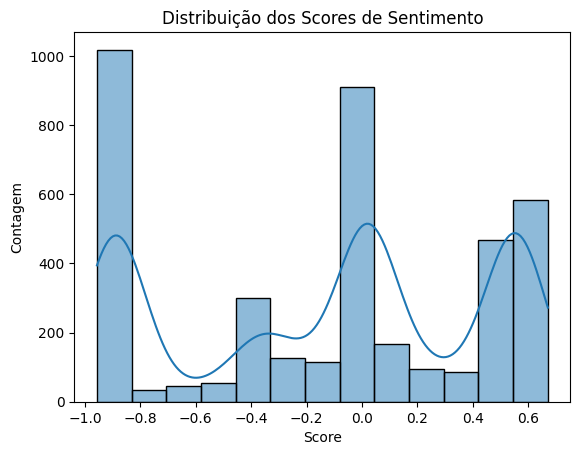
\includegraphics[scale=0.90]{images/score_distribution.png}
	\fautor
\end{figure}

Após obter o score de sentimento de cada postagem, o próximo passo foi agregar as postagens de cada usuário. Ao calcular a média ponderada do score de sentimento pelo número de postagens, conseguimos criar um score geral que reflete o sentimento médio de todas as postagens de um usuário. Esta métrica agregada nos forneceu uma visão mais clara do panorama geral dos sentimentos expressos nas redes de Niterói, Santo André e Mesquita.

\begin{figure}[htbp]
	\centering
	\begin{subfigure}{0.45\textwidth}
		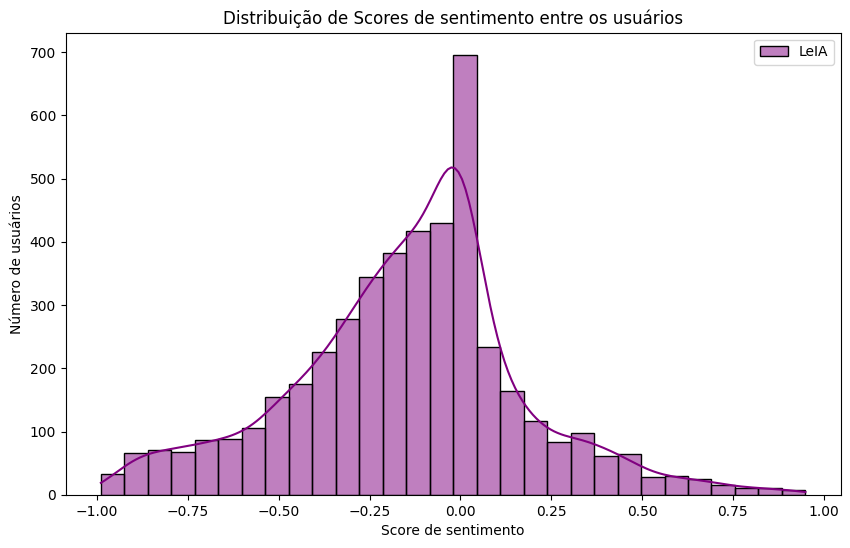
\includegraphics[width=\linewidth]{images/average_leia_by_number_of_users.png}
		\caption{Score Composto LeIA}
		\label{fig:average_leia_by_number_of_users}
	\end{subfigure}
	\hfill
	\begin{subfigure}{0.45\textwidth}
		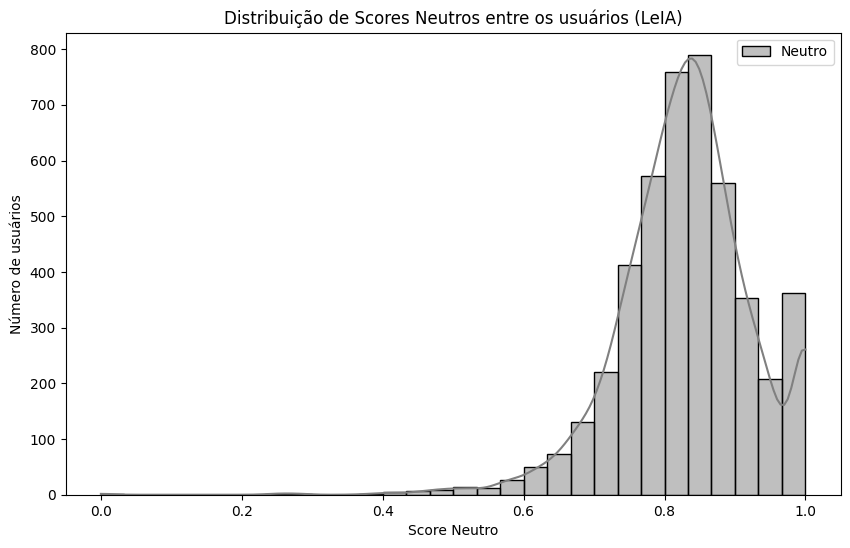
\includegraphics[width=\linewidth]{images/average_neutral_by_number_of_users.png}
		\caption{Neutros}
		\label{fig:average_neutral_by_number_of_users}
	\end{subfigure}
	\vskip\baselineskip
	\begin{subfigure}{0.45\textwidth}
		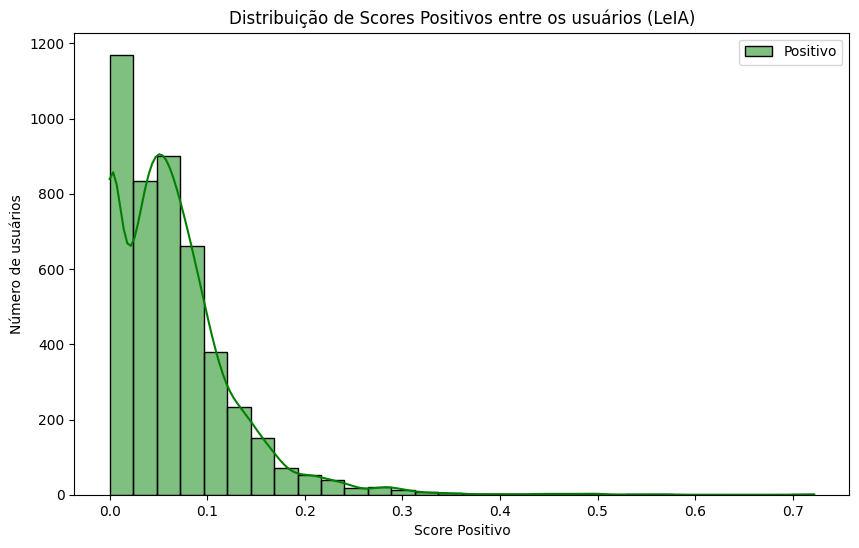
\includegraphics[width=\linewidth]{images/average_positive_by_number_of_users.png}
		\caption{Positivos}
		\label{fig:imagem3}
	\end{subfigure}
	\hfill
	\begin{subfigure}{0.45\textwidth}
		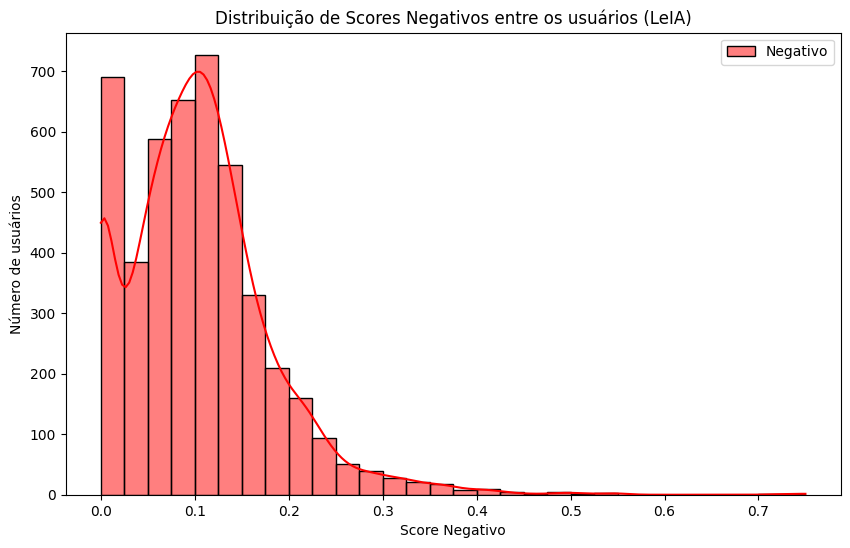
\includegraphics[width=\linewidth]{images/average_negative_by_number_of_users.png}
		\caption{Negativos}
		\label{fig:average_negative_by_number_of_users}
	\end{subfigure}
	\caption{Distribuição dos sentimentos médios em relação ao número de usuários. Os gráficos apresentam uma análise detalhada dos sentimentos, incluindo o score composto pelo LeIA, bem como as categorias neutras, positivas e negativas.}
	\label{fig:average_sentiment_by_number_of_users}
\end{figure}

Com os scores de sentimentos devidamente ajustados, partimos para uma análise mais detalhada dos dados. Uma observação inicial revelou que, ao contrário da premissa inicial de que a maioria das postagens tinha um tom negativo, a distribuição de sentimentos, quando consideramos cada postagem individualmente, mostra que 55.9\% das postagens são positivas, 24\% são negativas e 20.2\% são neutras. No entanto, quando agregamos todas as postagens de um único usuário, observamos que cerca de 67.3\% dos usuários têm postagens majoritariamente positivas, 17.7\% são majoritariamente negativas e 15\% são neutras.

Isso sugere que, embora possa haver uma percepção predominante de que os usuários expressam insatisfação ou preocupações em suas postagens, a realidade é mais matizada. A maioria dos usuários, de fato, tende a compartilhar feedbacks ou observações positivas sobre suas comunidades. Isso pode ser um reflexo de uma série de fatores: talvez os usuários estejam mais inclinados a compartilhar experiências positivas para promover a coesão comunitária, ou talvez as plataformas de mídia social, como o Colab, estejam se tornando espaços onde as pessoas desejam destacar o que está funcionando bem, em vez de apenas apontar problemas.

No entanto, os 24\% de postagens negativas não devem ser negligenciados. Mesmo que representem uma minoria em relação às postagens positivas, elas são cruciais para entender as áreas de preocupação e insatisfação dos usuários. Essas postagens podem ser extremamente valiosas para os tomadores de decisão, pois fornecem insights diretos sobre onde as intervenções podem ser mais necessárias.

As postagens neutras, que compõem 20.2\% do total, também são intrigantes. Elas podem representar uma variedade de conteúdos, desde solicitações de informação até comentários que não expressam uma opinião clara em uma direção ou outra. Essas postagens podem servir como um lembrete de que nem todo feedback pode ser facilmente categorizado como positivo ou negativo, e que a neutralidade em si pode oferecer insights sobre as áreas onde os sentimentos dos usuários são mistos ou incertos.

\begin{figure}[!htb]
	\caption{Scores de sentimento por quantidade de postagens}
	\label{fig:pie_sentiment_breakdown}
	\centering
	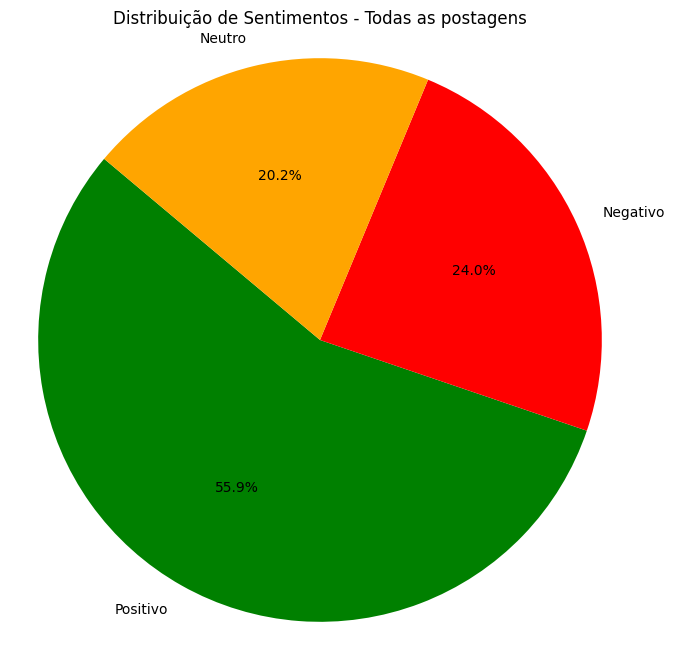
\includegraphics[scale=0.9]{images/pie_sentiment_breakdown.png}
	\fautor
\end{figure}

Ao analisar os eventos postados, observamos que "Entulho na calçada/via pública" é um dos tópicos mais frequentemente mencionados, com um total de 44.273 postagens. No entanto, é interessante notar que a maioria dessas postagens é classificada como neutra, com 35.391 postagens, seguida por 5.712 postagens positivas e 3.170 postagens negativas. Isso sugere que, embora haja uma alta incidência de relatos sobre entulho nas vias, muitos usuários não expressam uma opinião fortemente positiva ou negativa sobre o assunto.

Outro evento que se destaca é "Lâmpada apagada à noite", com um total de 8.701 postagens. Deste total, 3.212 postagens foram classificadas como neutras, 2.296 como positivas e 3.193 como negativas. Isso indica que há uma divisão nas opiniões dos usuários sobre a questão da iluminação pública à noite, com muitos reconhecendo os esforços para resolver o problema, mas também uma quantidade significativa de postagens expressando insatisfação.

Por outro lado, "Ponto de travessia irregular" teve um total de 46 postagens, das quais 31 foram classificadas como negativas, 6 como neutras e 6 como positivas. Isso sugere que há uma preocupação predominante com a segurança dos pontos de travessia, e que muitos usuários veem isso como uma área que precisa de melhorias.

Em resumo, os dados refletem as preocupações dos cidadãos em relação a diferentes aspectos da infraestrutura e serviços públicos. Enquanto alguns eventos são amplamente reportados e recebem uma mistura de feedback positivo, negativo e neutro, outros eventos, embora menos frequentemente mencionados, destacam-se por ter uma opinião predominantemente negativa ou positiva.

\begin{figure}[!htb]
	\caption{Distribuição dos 10 eventos mais comuns nas redes das 3 cidades.}
	\label{fig:pie_most_common_events}
	\centering
	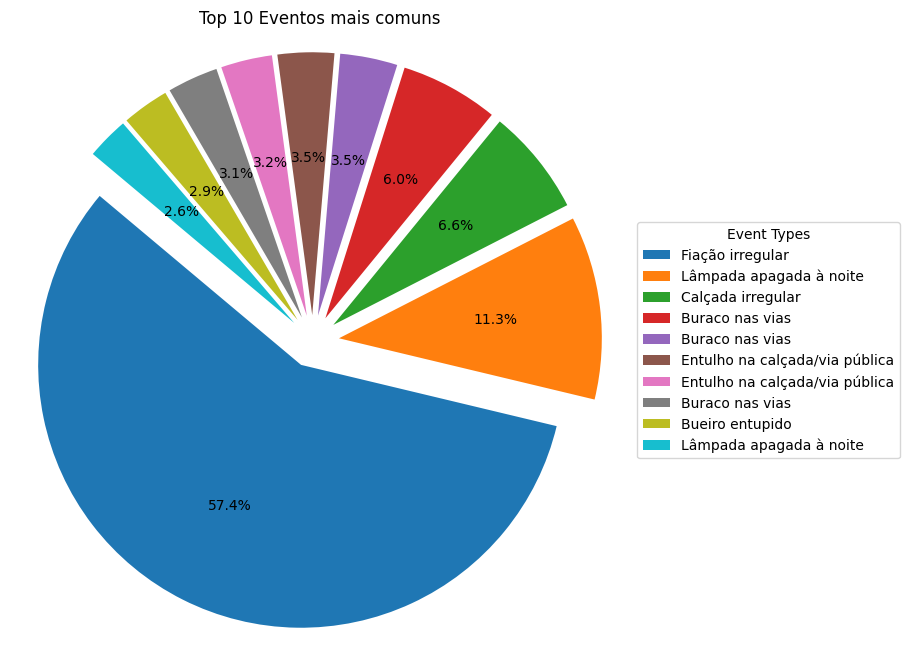
\includegraphics[scale=0.75]{images/pie_most_common_events.png}
	\fautor
\end{figure}

Ao expandir nossa análise para considerar a dimensão de gênero, observamos padrões distintos na distribuição de sentimentos entre diferentes grupos. Para as usuárias identificadas como femininas, notamos que a maioria das postagens (8.207) tem um sentimento negativo, seguido por 3.894 postagens positivas e 3.531 neutras. Isso sugere que, embora as mulheres estejam ativamente envolvidas na plataforma, elas tendem a expressar mais preocupações ou insatisfações em suas postagens do que sentimentos positivos ou neutros. Os usuários masculinos, por outro lado, apresentam um padrão diferente. Com 56.011 postagens neutras, 34.836 negativas e 22.513 positivas, vemos que a maioria das postagens masculinas é neutra. Isso pode indicar que os homens na plataforma tendem a ser mais informativos ou questionadores em suas postagens, sem expressar uma opinião clara em uma direção ou outra. Quanto aos usuários não binários, a amostra é extremamente pequena, com apenas uma postagem neutra registrada. Isso pode ser devido a uma representação limitada desse grupo na plataforma ou à relutância em se identificar devido a preocupações de privacidade. Os usuários que optaram por não informar seu gênero ou se identificaram como "outros" também têm uma presença na plataforma, embora em números menores em comparação com os gêneros masculino e feminino. Para os não informados, a distribuição é de 101 postagens negativas, 42 positivas e 37 neutras. Já para os que se identificam como "outros", temos 1.780 postagens negativas, 526 positivas e 1.356 neutras.

Essa análise por gênero destaca a importância de considerar as diversas perspectivas e experiências dos usuários ao avaliar o sentimento nas postagens. Cada grupo traz uma lente única para a plataforma, e entender essas nuances pode ajudar a criar estratégias de engajamento mais eficazes e a responder de forma mais adequada às preocupações e feedbacks dos usuários.

\begin{figure}[!htb]
	\caption{Distribuição dos scores de sentimento por gênero.}
	\label{fig:sentiment_by_gender}
	\centering
	\includegraphics[scale=0.8]{images/sentiment_by_gender.png}
	\fautor
\end{figure}

Aprofundando ainda mais nossa análise, decidimos explorar a relação entre a análise de sentimentos e a estrutura da rede social do Colab. A ideia era entender como os sentimentos expressos nas postagens poderiam influenciar ou ser influenciados pelas conexões e interações entre os usuários. Neste contexto, a análise de redes sociais, combinada com a análise de sentimentos, pode oferecer insights valiosos sobre a formação e a dinâmica de câmaras de eco dentro da plataforma.

Um conceito fundamental na análise de redes é a assortatividade, que mede a tendência de nós em uma rede se conectarem a outros nós que são semelhantes em alguma característica específica. No nosso caso, estávamos interessados em entender se usuários com sentimentos semelhantes tendem a se conectar e interagir mais entre si.

\begin{table}[h]
	\centering
	\begin{tabular}{|l|c|}
		\hline
		\textbf{Atributo} & \textbf{Valor de Assortatividade} \\
		\hline
		Tipo de Evento    & 0.015                             \\
		\hline
		Idade             & 0.015                             \\
		\hline
		Gênero            & 0.025                             \\
		\hline
		Escolaridade      & 0.01987                           \\
		\hline
		Raça              & 0.025                             \\
		\hline
		Score Lexicon     & 0.01489                           \\
		\hline
		Score Composto    & 0.01489                           \\
		\hline
		Score Positivo    & 0.01487                           \\
		\hline
		Score Negativo    & 0.01489                           \\
		\hline
		Score Neutro      & 0.01489                           \\
		\hline
		Cidade            & 0.02506                           \\
		\hline
	\end{tabular}
	\caption{Assortatividade por Atributo}
\end{table}

Para entender a influência dos sentimentos nas conexões entre os usuários, começamos por calcular a assortatividade da rede em relação a várias características, incluindo o tipo de evento, idade, gênero, educação, raça, score médio de sentimento e cidade. A assortatividade nos fornece uma métrica quantitativa que indica se a rede exibe uma tendência de homofilia, ou seja, se nós semelhantes tendem a se conectar entre si.

Os resultados foram reveladores. Os resultados foram reveladores. A assortatividade para todas as características listadas variou entre 0.01487 e 0.02506, indicando uma tendência moderada de homofilia na rede. Em outras palavras, há uma leve tendência para usuários com características semelhantes se conectarem entre si.

O atributo 'gênero' e 'raça' apresentaram valores de assortatividade de 0.025, sugerindo que os usuários tendem a se conectar mais frequentemente com outros usuários do mesmo gênero ou raça. Da mesma forma, o atributo 'cidade' também apresentou um valor semelhante de 0.02506, indicando que os usuários têm uma propensão a se conectar com outros que residem na mesma cidade. Isso era esperado, pois é natural que usuários da mesma cidade tenham mais probabilidade de se conectar e interagir entre si, dada a proximidade geográfica e os problemas comuns enfrentados.

Estes resultados têm implicações significativas para a dinâmica da rede social do Colab. A formação de câmaras de eco, especialmente em relação ao sentimento expresso nas postagens, pode influenciar a disseminação de informações, a percepção dos problemas e as soluções propostas. Por exemplo, se um grupo de usuários consistentemente posta com um sentimento negativo sobre um determinado tipo de evento, isso pode influenciar a percepção de outros usuários sobre a gravidade ou prevalência desse problema. Além disso, a presença de câmaras de eco pode ter implicações para a eficácia das intervenções ou políticas implementadas com base no feedback dos usuários. Se a plataforma estiver dominada por vozes particularmente positivas ou negativas, isso pode distorcer a percepção dos tomadores de decisão sobre as necessidades e prioridades da comunidade.

\begin{figure}[!htb]
	\caption{Assortatividade por Atributo}
	\label{fig:assortativity_by_attribute}
	\centering
	\includegraphics[scale=0.75]{images/assortativity_by_attribute.png}
	\fautor
\end{figure}

Ao analisar os dez usuários com o maior número de postagens na rede, podemos identificar padrões e características que nos ajudam a entender melhor a dinâmica da plataforma e os comportamentos dos usuários mais ativos. Estes usuários, devido à sua alta atividade, têm o potencial de influenciar significativamente a percepção e o sentimento geral da comunidade.

\begin{table}[h]
	\centering
	\caption{Detalhes dos usuários mais ativos}
	\begin{tabular}{|c|c|c|c|c|c|c|c|c|}
		\hline
		ID     & Centralidade & Seguidores & Seguindo & Eventos & Score & Gênero & Idade & Raça \\
		\hline
		318649 & 0.0585          & 24         & 5        & 12287.0   & -0.011      & M      & 38    & -    \\
		\hline
		240336 & 0.0532          & 13         & 4        & 11609.0   & 0.03        & M      & 49    & P    \\
		\hline
		425243 & 0.0422          & 15         & 15       & 5310.0    & -0.001      & M      & 48    & P    \\
		\hline
		216238 & 0.1354          & 72         & 17       & 4490.0    & -0.055      & M      & 59    & P    \\
		\hline
		186310 & 0.2552          & 133        & 406      & 4185.0    & -0.052      & M      & 52    & N    \\
		\hline
		76184  & 0.0447          & 74         & 56       & 4031.0    & -0.079      & M      & 31    & N    \\
		\hline
		43341  & 0.0261          & 64         & 24       & 3621.0    & -0.165      & M      & 40    & B    \\
		\hline
		194422 & 0.0234          & 28         & 14       & 2911.0    & -0.329      & O      & 28    & -    \\
		\hline
		253059 & 0.0624          & 26         & 6        & 1698.0    & 0.082       & M      & 48    & B    \\
		\hline
		200628 & 0.0341          & 43         & 0        & 1550.0    & -0.393      & M      & 36    & B    \\
		\hline
	\end{tabular}
\end{table}

Os dois usuários que lideram em número de postagens, com IDs 318649 e 240336, demonstram uma presença significativa na rede, com 12287 e 11609 postagens, respectivamente. No entanto, a influência na rede não se restringe apenas ao volume de postagens. A centralidade de autovetor, que indica a influência de um nó na rede, mostra que o usuário com ID 186310, apesar de estar em quinto lugar em número de postagens, é um dos mais influentes, com uma centralidade de 0.2552. Este usuário destaca-se não só pela sua influência, mas também pelo seu alto número de seguidores, 133, e pelo fato de seguir 406 outros usuários.

O sentimento geral das postagens, representado pelo score médio, varia entre os usuários. Por exemplo, enquanto o usuário com ID 253059 tem um score médio positivo de 0.082, indicando uma tendência a postagens mais positivas, o usuário com ID 194422 tem o score mais negativo de -0.329, sugerindo postagens com um tom mais crítico ou descontente.

Além disso, é interessante observar a diversidade demográfica entre os usuários mais ativos. Temos representantes de diferentes faixas etárias, desde os 28 anos do usuário com ID 194422 até os 59 anos do usuário com ID 216238. Em termos de raça, há uma variedade, com usuários identificados como brancos, negros e pardos. O gênero predominante entre os mais ativos é masculino, com uma exceção identificada como "outros".

A presença de uma ampla gama de scores de sentimento entre os usuários mais ativos é uma indicação saudável de uma comunidade vibrante e multifacetada. Em muitas plataformas online, é comum encontrar usuários que repetidamente postam conteúdo com uma única tonalidade, seja ela positiva, negativa ou neutra. No entanto, a diversidade observada aqui sugere que esses usuários estão engajados em uma variedade de tópicos e situações, refletindo uma gama mais ampla de experiências e sentimentos.

Além disso, essa variedade pode ser vista como um indicativo de autenticidade. Usuários que consistentemente postam com um único tom podem ser percebidos como tendenciosos ou até mesmo como bots. Por outro lado, aqueles cujas postagens refletem uma variedade de sentimentos são mais propensos a serem vistos como genuínos e confiáveis por outros membros da comunidade.

Isso também destaca a importância de não fazer suposições apressadas sobre os usuários com base apenas em sua atividade. Enquanto um alto volume de postagens pode sugerir um usuário muito engajado, a verdadeira natureza de seu engajamento só pode ser compreendida ao se considerar o conteúdo e o sentimento dessas postagens.

A diversidade de sentimentos também pode ser um indicativo de que a plataforma está servindo a seu propósito de fornecer um espaço para discussão e feedback. Se todos os usuários mais ativos tivessem sentimentos uniformemente positivos ou negativos, poderia ser um sinal de que a plataforma está se tornando uma câmara de eco, onde apenas certas opiniões são expressas e reforçadas.

Além disso, essa diversidade pode ser benéfica para os administradores ou moderadores da plataforma. Ao monitorar os sentimentos variados dos usuários mais ativos, eles podem obter insights valiosos sobre áreas de preocupação, bem como aspectos da plataforma ou da comunidade que estão funcionando bem. Isso pode informar decisões sobre modificações na plataforma, campanhas de engajamento ou iniciativas de moderação.

Por fim, é essencial reconhecer que, em qualquer comunidade, a diversidade de opiniões e experiências enriquece o diálogo e a troca de ideias. A presença de usuários ativos com uma variedade de sentimentos sugere uma comunidade dinâmica e engajada, onde os membros se sentem livres para expressar suas opiniões e compartilhar suas experiências, sejam elas positivas, negativas ou neutras.

\begin{figure}[!htb]
	\caption{Eigencentrality vs. Número de Posts}
	\label{fig:eigencentrality_vs_number_of_posts}
	\centering
	\includegraphics[scale=0.70]{images/eigencentrality_vs_number_of_posts.png}
	\fautor
\end{figure}

Ao longo deste experimento, exploramos a o complexo microcosmo representado pelos sentimentos e opiniões expressas pelos usuários da plataforma Colab. A análise de sentimentos, quando aplicada a plataformas de mídia social, pode revelar insights profundos sobre as percepções, preocupações e satisfações dos usuários. No caso do Colab, essa análise nos permitiu entender melhor a dinâmica da comunidade e as emoções subjacentes às postagens dos usuários.

Primeiramente, a presença de uma distribuição quase equilibrada de sentimentos positivos e negativos desafia a noção comum de que plataformas de feedback tendem a ser dominadas por críticas. Isso sugere que o Colab não é apenas um espaço para reclamações, mas também um fórum onde os usuários reconhecem e apreciam as soluções e melhorias.

A análise dos usuários mais ativos e suas postagens revelou uma diversidade saudável de sentimentos, refutando a ideia de que os usuários mais ativos são unidimensionais em suas postagens. Esta diversidade é um testemunho da autenticidade e do engajamento genuíno dos usuários com a plataforma. Além disso, destaca a importância de considerar o conteúdo e o sentimento das postagens, em vez de se basear apenas no volume de atividade.

A presença de câmaras de eco, onde usuários com sentimentos semelhantes tendem a se agrupar, é uma preocupação em muitas plataformas online. No entanto, a diversidade de sentimentos observada no Colab sugere que a plataforma tem evitado, até certo ponto, essa armadilha. Isso é crucial para garantir que a plataforma continue a ser um espaço para discussão aberta e feedback construtivo.

A análise de redes sociais combinada com a análise de sentimentos também revelou padrões interessantes de conexão e interação entre os usuários. A tendência de usuários com sentimentos semelhantes se conectarem entre si tem implicações significativas para a disseminação de informações e a formação de opiniões dentro da plataforma.

Em conclusão, a análise de sentimentos no Colab ofereceu uma janela única para o coração e a mente da comunidade. Revelou uma comunidade vibrante e engajada, onde os membros se sentem empoderados para expressar suas opiniões e compartilhar suas experiências. À medida que a plataforma continua a crescer e evoluir, será essencial continuar monitorando e compreendendo esses sentimentos para garantir que o Colab permaneça um espaço inclusivo, autêntico e valioso para todos os seus membros.

Até o momento, nossa abordagem para a análise de sentimentos nas postagens do Colab foi baseada em técnicas manuais e ferramentas como o NLTK. Embora tenhamos obtido insights valiosos e estabelecido um score para cada postagem, é evidente que essa metodologia possui limitações em termos de escalabilidade e sustentabilidade, especialmente considerando o volume crescente de dados gerados diariamente na plataforma. Para superar esses desafios e otimizar o processo de análise de sentimentos, é imperativo adotar uma abordagem mais automatizada e robusta. Neste contexto, o aprendizado de máquina emerge como uma solução promissora. Ao utilizar um subconjunto das postagens que já classificamos manualmente - um conjunto de treinamento de aproximadamente 4.000 postagens - podemos treinar um modelo de aprendizado de máquina para realizar a classificação de sentimentos de forma autônoma. Esta abordagem não apenas acelera o processo de análise, mas também garante uma maior consistência e precisão na classificação. No próximo segmento, exploraremos em detalhes a implementação e os benefícios desta metodologia baseada em aprendizado de máquina, delineando como ela pode melhorar nossa capacidade de entender e interpretar os sentimentos expressos pelos usuários do Colab.

\section{Análise de Sentimento usando Regressão Supervisionada}

Nessa seção, descrevemos a metodologia empregada para a análise de dados e a construção do modelo de aprendizado de máquina e apresentamos uma abordagem para realizar a análise de sentimento em postagens do Colab. Este modelo foi treinado usando um conjunto de dados de treinamento que consiste em postagens de usuário rotuladas como positivas ou negativas. O modelo então aprende a associar certas palavras e frases a sentimentos positivos ou negativos.

A distinção entre classificação e regressão é um pilar central no aprendizado de máquina supervisionado. A classificação é destinada à atribuição de categorias discretas a instâncias de dados, ao passo que a regressão prediz elementos contínuos, oferecendo um espectro de possibilidades (\citeonline{2017_Shen_IC}).

No domínio da análise de sentimentos, a prática convencional muitas vezes simplifica a complexidade dos sentimentos humanos a categorias binárias. Todavia, sentimentos são intrinsecamente graduais e multidimensionais. Ao adotar uma escala contínua de -1 a 1 para representar sentimentos, abraçamos a sutileza e a riqueza dessas variações.

A opção pela regressão como abordagem modelagem foi catalisada pelos insights revelados na análise exploratória de sentimentos do capítulo anterior, na qual identificamos um espectro completo de sentimentos. Preservar essa continuidade permite-nos capturar as nuances mais finas nas postagens, concedendo-nos também a flexibilidade para futuras adaptações metodológicas sem a perda de detalhes valiosos dos dados originais.

Para fortalecer nosso conjunto de dados de treinamento e expandir nossa compreensão dos sentimentos manifestados nas postagens do Colab, incluímos uma seleção aleatória de 2000 eventos adicionais. Esta estratégia promove a diversidade e representa melhor a gama de sentimentos expressos, evitando vieses que poderiam surgir da seleção de extremos. Combinando esses eventos com os dados das postagens das três cidades estudadas anteriormente, consolidamos um conjunto de treinamento robusto com 4000 instâncias.

Esperamos que o algoritmo, ao ser treinado com essa rica fonte de dados, aprenda a correlacionar padrões linguísticos com sentimentos positivos ou negativos, propiciando uma classificação automática refinada dos sentimentos nas postagens do Colab. Esta abordagem de aprendizado supervisionado utiliza os dados de treinamento como alicerces para a criação de um modelo generalista capaz de captar a gama de sentimentos expressos nas postagens.

Depois da extração de recursos e da análise exploratória, dividimos os dados em conjuntos de treino e validação, seguido pela padronização dos mesmos para assegurar uniformidade na escala (\cite{2000_Jain}). Testamos uma gama de modelos regressivos para discernir o mais apropriado para nossa aplicação:

\begin{itemize}
\item \textbf{RandomForestRegressor}: Este algoritmo constrói um ensemble de árvores de decisão e usa a média de suas previsões para gerar o resultado final. É notável pela sua robustez em lidar com grandes volumes de dados e pela habilidade em captar interações complexas entre as variáveis, minimizando o risco de overfitting \cite[5-32]{2001_Breiman}.
\item \textbf{LinearRegression}: Um dos métodos mais fundamentais e amplamente aplicados, a Regressão Linear busca estabelecer uma relação linear entre variáveis dependentes e independentes.
\item \textbf{DecisionTreeRegressor}: Este modelo segmenta o espaço de dados em subconjuntos baseados em características e utiliza a média dos valores dos subconjuntos para fazer previsões. Sua interpretabilidade é uma vantagem, embora possa sucumbir ao overfitting se não for devidamente ajustado \cite[81-106]{1986_Quinlan}.
\item \textbf{K-Nearest Neighbors (KNN)}: O KNN faz previsões com base na semelhança entre instâncias de dados, considerando os 'k' exemplos mais próximos no conjunto de treinamento para inferir resultados.
\end{itemize}

Em um campo desafiador como a análise de sentimentos, especialmente quando focado na identificação de câmaras de eco, é imperativo selecionar um modelo de aprendizado de máquina que possa capturar com precisão a gama de sentimentos nos dados. Avaliamos o desempenho dos modelos utilizando métricas como MSE, MAE e o coeficiente de determinação (R\^2), que são mais indicativas do que a acurácia para tarefas de regressão.

O Random Forest Regressor destaca-se como a opção mais promissora, exibindo um equilíbrio ideal entre acurácia e generalização. O Decision Tree Regressor, apesar de um R\^2 quase perfeito no treinamento, evidencia overfitting devido à discrepância em validação. O KNN não alcançou o desempenho esperado em comparação aos outros modelos.

Em análise de sentimentos, a precisão é um desiderato, especialmente ao explorar dinâmicas sociais em plataformas como o Colab. Iniciamos este capítulo com um experimento nas mensagens dos usuários de três cidades, utilizando uma heurística baseada em dicionários de sentimentos, polaridade de emojis e ferramentas como o LeIA. A transparência dessa metodologia inicial é uma vantagem, mas também pode introduzir vieses. O trânsito para um modelo de aprendizado de máquina, especificamente o Random Forest, tem como objetivo mitigar tais vieses e melhorar a objetividade.

A preparação e a qualidade dos dados são vitais para o sucesso do modelo de aprendizado. Ao utilizar os scores de sentimentos do experimento inicial como entradas para o modelo regressivo, estabelecemos um processo sequencial e integrado de análises. Este estudo sublinha a importância de métodos adaptáveis na análise de sentimentos, especialmente ao lidar com fenômenos sociais complexos. Com os insights adquiridos, o próximo passo é classificar os usuários em personas, utilizando o score de sentimentos, tópicos de interesse e modelos de classificação para desvelar as tendências de polarização e interação no Colab.

\begin{table}[h]
	\centering
	\begin{tabular}{|l|c|c|c|c|c|c|}
		\hline
		\textbf{Modelo} & \textbf{Training R$^2$} & \textbf{Validation R$^2$} & \textbf{MSE} & \textbf{MAE} & \textbf{RMSE} & \textbf{Tempo (s)} \\
		\hline
		Random Forest   & 0.9619                  & 0.7228                    & 0.0847       & 0.1683       & 0.2910        & 1192.96            \\
		\hline
		Decision Tree   & 0.9999                  & 0.5107                    & 0.1496       & 0.1894       & 0.3867        & 33.65              \\
		\hline
		KNN             & 0.4932                  & 0.1727                    & 0.2529       & 0.3871       & 0.5029        & 133.97             \\
		\hline
	\end{tabular}
	\caption{Desempenho dos modelos de regressão nos dados de treinamento e validação.}
	\label{tab:model_performance}
\end{table}	

A partir desses resultados, podemos concluir que o Random Forest Regressor é o modelo mais promissor entre os testados, com o melhor equilíbrio entre desempenho nos dados de treinamento e validação. O Decision Tree Regressor parece estar overfitting, dado o R\^2 quase perfeito nos dados de treinamento e o desempenho significativamente pior nos dados de validação. O KNN, por outro lado, tem um desempenho geralmente mais fraco em comparação com os outros modelos.

A análise de sentimentos, particularmente em plataformas dinâmicas como o Colab, é uma tarefa intrincada que exige uma abordagem meticulosa. No início deste capítulo, conduzimos um experimento para classificar as mensagens dos usuários de Niterói, Santo André e Mesquita. Utilizando uma heurística baseada em dicionários léxicos, polaridade de emojis e a ferramenta LeIA, atribuímos scores de sentimentos às postagens. Este processo é transparente, permitindo-nos codificar cada etapa da atribuição de scores como uma caixa branca. No entanto, essa transparência também pode introduzir viéses, sejam eles conscientes ou não.

A decisão de transformar essa abordagem inicial em um modelo de aprendizado de máquina foi motivada pela perspectiva da engenharia de software. Ao adotar a regressão supervisionada, buscamos criar um sistema mais objetivo e menos suscetível a viéses humanos. A escolha do Random Forest Regressor, que demonstrou desempenho superior, reitera a necessidade de algoritmos robustos para capturar padrões complexos nos dados. Além disso, manter os scores de sentimento em um espectro contínuo, em vez de categorias discretas, permitiu uma representação mais fiel e granular dos sentimentos.

A qualidade dos dados e sua preparação são fundamentais para o sucesso de qualquer modelo de aprendizado de máquina. Ao usar os scores de sentimentos derivados do experimento inicial como insumo para o treinamento do modelo de regressão, demonstramos a interconexão e a sequencialidade dos experimentos. Esta pesquisa destaca a importância de abordagens adaptativas em análise de sentimentos, especialmente ao abordar fenômenos sociais complexos. Com os insights obtidos através desta modelagem de sentimentos, o próximo passo é a classificação dos usuários em personas. Utilizando o score de sentimento, os tópicos mais comentados e um modelo de classificação, buscaremos entender melhor os perfis dos usuários. Esta compreensão será crucial para a subsequente análise de redes, visando a detecção de câmaras de eco e aprofundando nossa compreensão sobre as dinâmicas de interação e polarização no Colab.

\section{Análise de Sentimento e Personas: Uma Nova Perspectiva sobre as Postagens do Colab}

Nossa jornada analítica no Colab começou com uma avaliação meticulosa das interações dos usuários, empregando técnicas sofisticadas de processamento de linguagem natural e análise de redes. Este processo gerou um sistema de pontuação capaz de capturar a polaridade dos sentimentos - positivos, negativos ou neutros - em cada postagem. Esta avaliação considerou não só o léxico e emojis utilizados, mas também os jargões e nuances específicas da plataforma.

Este sistema não só desvendou a natureza das interações na plataforma, revelando tendências e sentimentos dominantes, como também permitiu, ao ser combinado com análise de redes, vislumbrar a disseminação de sentimentos através das conexões entre os usuários. Esta sinergia entre análise de sentimentos e de redes elucidou a dinâmica complexa das interações comunitárias.

Com a análise de sentimentos estabelecida, o foco ampliou-se naturalmente para a classificação de personas, com o intuito de decifrar padrões comportamentais mais abrangentes dos usuários. Esta etapa avançada da pesquisa almejou transcender a análise individual de postagens para compreender como os usuários, em suas conexões e influências mútuas, coalescem em arquétipos mais amplos - as personas.

Essas personas são construções representativas que sintetizam os traços e comportamentos de grupos de usuários. No ecossistema do Colab, identificamos principalmente duas personas: os \textit{helpers} e os \textit{complainers}. Os Helpers se caracterizam pelo engajamento colaborativo e proativo, frequentemente auxiliando e partilhando informações valiosas. Já os Complainers tendem a adotar uma postura mais crítica, expressando descontentamento e críticas frequentes.

Ambas as personas são fundamentais para a dinâmica do Colab. Os Helpers fomentam o apoio mútuo e a resolução colaborativa de problemas, enquanto os Complainers podem ser catalisadores de mudança, destacando áreas que necessitam de atenção e melhoria. Contudo, quando essas personas se polarizam, surgem riscos de formação de câmaras de eco, locais onde as opiniões se reforçam mutuamente, limitando a diversidade de perspectivas.

Através da análise de sentimentos e subsequente classificação em personas, procuramos desvendar como os usuários se distribuem na rede do Colab e os padrões emergentes. Esse entendimento é crucial para identificar a existência de "bolhas de personas" e para investigar a dinâmica que as sustenta: Será um fenômeno intrínseco ao comportamento dos usuários ou as plataformas de mídia social estão, através de viéses algorítmicos, contribuindo ativamente para essa segregação? No decorrer desta seção, abordaremos as metodologias aplicadas para discernir e classificar as personas \textit{helpers} e \textit{complainers} no Colab. Ao aprofundar-se na implementação desses arquétipos, realçaremos sua relevância para a análise de dados e para o aprimoramento estratégico da plataforma.

\subsubsection*{Helpers}

A persona \textit{helper} é caracterizada por um comportamento proativo e colaborativo em uma comunidade online. Esses indivíduos são frequentemente encontrados respondendo a perguntas, oferecendo conselhos e compartilhando informações úteis com outros membros da comunidade. Eles tendem a expressar sentimentos positivos em suas postagens e são motivados pelo desejo melhorar o coletivo e contribuir para a comunidade.

No Colab, por exemplo, muitos usuários realizam postagens frequentes reportando buracos nas vias, estruturas danificadas, alertam para situações de alagamento e deslizamento de terrenos. Muitos desses usuários adotam formatos padronizados para suas postagens, incluindo fotos, localização e descrição detalhada do problema. Além disso, eles frequentemente interagem com outros usuários, fornecendo informações adicionais ou atualizações sobre o status do problema.

Os \textit{helpers} são fundamentais para o sucesso de qualquer comunidade online, pois eles ajudam a criar um ambiente de apoio e colaboração. Eles são frequentemente vistos como líderes informais ou especialistas em suas respectivas áreas de interesse. Eles podem ser motivados por uma variedade de fatores, incluindo o desejo de compartilhar conhecimento, a satisfação de ajudar os outros, ou o reconhecimento e respeito que recebem da comunidade.

\subsubsection*{Complainers}

A persona \textit{complainer} é caracterizada por um comportamento mais crítico ou negativo em uma comunidade online. Esses indivíduos são frequentemente encontrados expressando insatisfação, fazendo reclamações ou criticando ações das agências públicas. Eles tendem a expressar sentimentos negativos em suas postagens e são motivados por uma variedade de fatores, incluindo frustração, descontentamento ou a necessidade de expressar suas opiniões. Também é importante notar que a maioria das postagens de \textit{complainers} não são necessariamente negativas, pois os usuários estão de fato reportando problemas nas cidades, mas podem ser percebidas como tal devido ao seu tom ou conteúdo. Um outro fator interessante é que muitas das postagens de \textit{complainers} são direcionadas a assuntos mais individualizados como reportes nas vicinidades de suas residências ou locais de trabalho. Notavelmente ao analisar os comentários, esses usuários tendem a comentar ativamente em postagens criadas por outros usuários, muitas vezes expressando apoio ou concordância com o autor da postagem, mas sempre destacando a ineficiência ou ineficácia dos órgãos públicos.

No Colab, muitos usuários realizam postagens se referindo a prefeitura e outros órgãos sarcasticamente, fazendo críticas e reclamações sobre a falta de manutenção de vias, atrasos em obras, entre outros. Outro ponto recorrente diz respeito a perturbação sonora e uma certa correlação com alguns preconceitos musicais. Alguns usuários com scores particularmente negativos tendem a cobrar os orgãos públicos pelos impostos pagos que são, na opinião desses usuários, mal administrados, assim como outras tarifas como de transporte público ou de energia elétrica.

Os \textit{complainers} desempenham um papel importante em qualquer comunidade online, pois eles ajudam a identificar problemas, desafios ou áreas de melhoria. Embora suas postagens possam ser percebidas como negativas, elas podem fornecer feedback valioso que pode ser usado para melhorar a comunidade. No entanto, é importante gerenciar e responder adequadamente a esses usuários para evitar a criação de um ambiente negativo ou tóxico.

\subsubsection*{O papel das personas na Comunidade do Colab}

A presença das personas \textit{helpers} e \textit{complainers} dentro do Colab é altamente relevante para o ecossistema dessa plataforma colaborativa. Ambas as personas desempenham papéis distintos e complementares que podem influenciar a experiência do usuário e fornecer insights valiosos para o aprimoramento contínuo do aplicativo. A seguir, são apresentados os argumentos que sustentam a relevância dessas personas específicas:

Os Helpers desempenham um papel fundamental no Colab, pois contribuem ativamente para a comunidade, oferecendo suporte, compartilhando conhecimento e fornecendo soluções para os desafios enfrentados pelos usuários. Eles ajudam a fomentar a colaboração e o aprendizado coletivo, tornando-se recursos valiosos para aqueles que precisam de assistência ou orientação. Sua presença cria um ambiente propício para troca de ideias, resolução de problemas e crescimento mútuo. Ao compartilhar suas habilidades e conhecimentos, os Helpers estabelecem uma cultura de generosidade e reciprocidade dentro da comunidade do Colab. Eles inspiram outros usuários a se envolverem ativamente, encorajando a participação e a colaboração entre os membros. Além disso, a presença de Helpers é essencial para garantir que novos usuários se sintam bem-vindos e apoiados, promovendo assim um ambiente inclusivo e acolhedor.

Embora os Complainers possam ser vistos como usuários críticos ou negativos, sua presença é igualmente importante para o Colab. Essas personas desempenham o papel de destacar problemas, lacunas e áreas de melhoria dentro do aplicativo. Ao expressar suas preocupações e insatisfações, eles fornecem um feedback valioso que pode impulsionar o aprimoramento contínuo da plataforma.

Os Complainers atuam como "sentinelas" da comunidade, chamando a atenção para questões que podem ter sido negligenciadas ou passado despercebidas. Suas críticas construtivas podem levar a melhorias significativas na usabilidade, funcionalidade e qualidade geral do Colab. Além disso, ao abordar e resolver essas preocupações, a equipe responsável pelo desenvolvimento do aplicativo demonstra seu compromisso com a satisfação e o engajamento dos usuários.

A interação entre as personas \textit{helpers} e \textit{complainers} no Colab é uma relação simbiótica que impulsiona o crescimento e o aprimoramento contínuo da plataforma. Os Helpers oferecem suporte, orientação e soluções, tornando o ambiente colaborativo e enriquecedor. Por outro lado, os Complainers fornecem feedback crítico e identificam áreas de melhoria, promovendo a evolução e aprimoramento do aplicativo. Essa sinergia entre essas personas complementares é essencial para criar uma comunidade vibrante, responsiva e em constante aprimoramento no Colab.

A partir de uma análise exploratória de sentimento, foram identificadas as personas \textit{helpers} e \textit{complainers} dentro do Colab. No entanto, é importante ressaltar que existem outras personas que também podem ser identificadas, como por exemplo, a persona "Explorer", que tem um perfil voltado para a exploração da cidade e reporte dos problemas identificados. Além disso, uma nova persona que poderia ser considerada é a persona "Innovator", alguém que está sempre em busca de novas soluções e ideias inovadoras para melhorar a experiência dos usuários no Colab. A escolha das duas personas mencionadas anteriormente foi baseada nossa capacidade de mensurar e classificar essas personas através da analise de sentimento de suas postagens e também em seu potencial de gerar câmaras de eco, pois representam posições mais antagônicas dentro das comunidades da rede.

Nas próximas páginas, detalharemos as técnicas e metodologias utilizadas para identificar e classificar as personas \textit{helpers} e \textit{complainers} dentro do Colab, fornecendo uma visão mais aprofundada sobre a implementação dessas personas e sua contribuição para a análise de dados e aprimoramento da plataforma.

\section{Classificação de usuário por Persona}

A construção de um modelo de classificação para análise de sentimentos em plataformas como o Colab é uma tarefa intrincada. A linguagem utilizada pelos usuários é repleta de nuances, jargões específicos, emojis e outros elementos que podem influenciar a interpretação do sentimento. Além disso, a diversidade demográfica dos usuários traz uma riqueza de perspectivas e formas de expressão. O principal desafio é desenvolver um modelo que seja sensível a essas nuances, evitando o overfitting, e que possa generalizar bem para postagens não vistas anteriormente.

Para assegurar uma representação abrangente e equitativa da comunidade do Colab, 5000 postagens foram meticulosamente selecionadas com base em critérios demográficos. Esta seleção garantiu que todas as faixas etárias, gêneros e raças estivessem representados de forma proporcional à distribuição desses grupos entre os usuários do aplicativo. Além disso, levamos em consideração o tamanho das postagens, garantindo uma mistura de postagens longas e curtas. Cada postagem foi então manualmente classificada como \textit{helper} ou \textit{complainer}, considerando-se o conteúdo, a intenção e as nuances da linguagem.

Do conjunto inicial de postagens, 4000 foram destinadas ao treinamento, mantendo um equilíbrio de 2000 postagens para cada categoria (\textit{helper} e \textit{complainer}). As 1000 postagens restantes foram reservadas como conjunto de teste. Esta separação assegura que o modelo seja treinado e avaliado em conjuntos distintos, minimizando o risco de overfitting.

\section{Treinamento do modelo de classificação de Personas}

A abordagem adotada para a análise de sentimentos e classificação de personas é orientada a objetos, o que facilita a modularização e reutilização do código. O código é estruturado em várias classes, cada uma com responsabilidades específicas. A classe SentimentClassifierModel é responsável pela carga de dados, pré-processamento, vetorização e treinamento de modelos de classificação de sentimentos. A vetorização é realizada usando o CountVectorizer, que converte o texto em uma matriz de contagens de termos/tokens. A classe também suporta vários tipos de modelos, incluindo Floresta Aleatória, Regressão Logística, Árvore de Decisão e KNN, permitindo flexibilidade na escolha do algoritmo. A classe ColabSentimentClassifier atua como uma camada de alto nível, integrando a análise de eventos do Colab com o modelo de classificação de sentimentos. Ela carrega os dados dos eventos, inicializa o modelo e atualiza os scores de sentimentos dos usuários. A classe PersonaClassifier é a peça central para a classificação de personas.

\begin{figure}
	\centering
	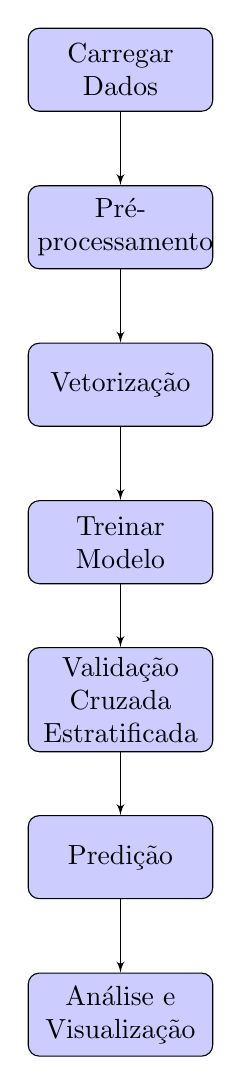
\begin{tikzpicture}[node distance=2cm, auto]
		% Estilos
		\tikzstyle{block} = [rectangle, draw, fill=blue!20, text width=6em, text centered, rounded corners, minimum height=3em]
		\tikzstyle{line} = [draw, -latex']
		% Nós
		\node [block] (init) {Carregar Dados};
		\node [block, below of=init] (preprocess) {Pré-processamento};
		\node [block, below of=preprocess] (vectorize) {Vetorização};
		\node [block, below of=vectorize] (train) {Treinar Modelo};
		\node [block, below of=train] (validate) {Validação Cruzada Estratificada};
		\node [block, below of=validate] (predict) {Predição};
		\node [block, below of=predict] (analysis) {Análise e Visualização};
		% Conexões
		\path [line] (init) -- (preprocess);
		\path [line] (preprocess) -- (vectorize);
		\path [line] (vectorize) -- (train);
		\path [line] (train) -- (validate);
		\path [line] (validate) -- (predict);
		\path [line] (predict) -- (analysis);

	\end{tikzpicture}
	\caption{Workflow de Classificação.}
\end{figure}

O código também enfatiza a importância da limpeza e pré-processamento de dados. Funções de preprocessamento são usadas para remover stopwords, realizar stemming e limpar caracteres indesejados. Esta etapa é crucial, pois a qualidade do texto de entrada pode afetar significativamente a performance do modelo. A abordagem modular e orientada a objetos adotada facilita a manutenção, extensão e compreensão do código, permitindo que pesquisadores e desenvolvedores ajustem e expandam facilmente as funcionalidades conforme necessário.

Para avaliar a robustez e a confiabilidade do modelo, foi empregada a técnica de validação cruzada estratificada, especificamente utilizando o método Stratified K-Fold com cinco divisões (folds). A estratificação, neste contexto, refere-se ao processo de dividir o conjunto de treinamento de forma que cada subconjunto (ou "fold") mantenha uma distribuição semelhante de \textit{helper} e \textit{complainer}. Esta técnica é essencial para garantir que o modelo seja avaliado de maneira justa e consistente, independentemente da divisão dos dados.

O método de avaliação do modelo realiza uma série de passos para avaliar a performance do modelo. Inicialmente, o modelo é treinado e avaliado em um conjunto de teste separado, com métricas como \textit{F1 Score}, \textit{Precision Score} e \textit{Misclassification Rate} sendo calculadas para o modelo como um todo. Posteriormente, a validação cruzada estratificada é aplicada, e o modelo é treinado e avaliado em cada fold. Métricas como Acurácia, AUC Score, Matriz de Confusão, \textit{F1 Score}, \textit{Precision Score} e \textit{Misclassification Rate} são calculadas para cada fold e, em seguida, são calculadas as médias dessas métricas para fornecer uma visão abrangente da performance do modelo. Além disso, o método também inclui a geração de curvas ROC e a classificação de posts não vistos, fornecendo insights adicionais sobre a capacidade do modelo em generalizar para dados novos. Ao final, uma heurística é aplicada para avaliar se o modelo está apresentando um bom desempenho, com considerações adicionais sobre os requisitos específicos da aplicação e o impacto prático dos erros do modelo.

Os resultados dessa validação, com acurácias consistentemente altas e outras métricas indicando bom desempenho, fornecem uma indicação da confiabilidade do modelo em fazer previsões precisas e confiáveis. Inicialmente criamos um modelo simples com um conjunto de trreinamento de 1000 postagens utilizando o classificador Random Forest. Com os testes preliminares realizados e o modelo demonstrando uma razoável capacidade de classificação, decidimos explorar e comparar diferentes algoritmos de aprendizado de máquina para avaliar seu desempenho em relação ao modelo original, baseado em Floresta Aleatória (Random Forest). Os modelos selecionados para a comparação são:

\begin{itemize}
    \item \textbf{Regressão Logística (Logistic Regression)}: Um modelo estatístico que utiliza a função logística para modelar a probabilidade de uma classe binária.
    \item \textbf{Naive Bayes Multinomial (Multinomial Naive Bayes)}: Uma extensão do algoritmo Naive Bayes que é adequada para variáveis de resposta multinomiais, comumente utilizado para classificação de texto.
    \item \textbf{XGBoost}: Um algoritmo de aprendizado de máquina baseado em árvore de decisão otimizado para desempenho e velocidade, que se destaca em competições de ciência de dados.
    \item \textbf{SVC (Support Vector Classifier)}: Um tipo de máquina de vetores de suporte que é utilizado para classificação.
    \item \textbf{KNeighborsClassifier}: Um algoritmo de aprendizado baseado em instância que classifica um objeto com base na maioria de votos de seus vizinhos mais próximos.
    \item \textbf{DecisionTreeClassifier}: Um modelo de aprendizado de máquina que utiliza uma árvore de decisão como modelo preditivo.
    \item \textbf{LightGBM}: Um framework de aumento de gradiente que utiliza algoritmos baseados em árvore, otimizado para eficiência e desempenho.
    \item \textbf{CatBoost}: Um algoritmo de aumento de gradiente categórico que é especialmente poderoso para lidar com recursos categóricos.
\end{itemize}

Cada um desses modelos possui características únicas e é aplicável a diferentes tipos de problemas, o que justifica a sua inclusão nesta comparação abrangente. Além disso, cada modelo possui um conjunto interno de parâmetros que afetam o processo de treinamento e modelagem. Conhecidos como \textit{hyperparameters}, ou hiperparâmetros, esses não são aprendidos durante o processo de treinamento, mas são definidos previamente. Eles influenciam a forma como o modelo vai aprender, podendo afetar a sua performance, a capacidade de generalização e a prevenção de overfitting ou underfitting. Os \textit{hyperparameters} podem incluir, por exemplo, a taxa de aprendizado em algoritmos de otimização, o número de árvores em uma floresta aleatória, o tipo de kernel em uma máquina de vetores de suporte (SVM), entre outros. A escolha adequada desses parâmetros é crucial, pois pode significativamente impactar a eficácia do modelo em fazer previsões precisas e confiáveis.

Para encontrar os melhores parâmetros para cada modelo, empregamos técnicas de otimização de hiperparâmetros, como Grid Search, Randomized Search e Bayesian Optimization. Essas técnicas exploram diferentes combinações de parâmetros, avaliando estatisticamente a performance do modelo para cada combinação, com o objetivo de identificar aqueles que maximizam a acurácia, ou outra métrica de interesse, do modelo. Grid Search realiza uma busca exaustiva sobre um conjunto predefinido de valores de hiperparâmetros, enquanto Randomized Search explora aleatoriamente as combinações de parâmetros, o que pode ser mais eficiente em espaços de busca grandes. Já a Bayesian Optimization constrói um modelo probabilístico da função objetivo e utiliza esse modelo para selecionar de forma inteligente os próximos candidatos a serem avaliados, buscando otimizar a função objetivo de forma mais eficiente. Ao final desse processo heurístico, obtemos um conjunto otimizado de hiperparâmetros que, quando aplicados aos modelos, buscam proporcionar uma performance superior e resultados mais confiáveis nas tarefas de classificação e previsão.

Em geral, observou-se que todos os modelos apresentaram métricas de desempenho similares, com curvas ROC comparáveis e acurácias próximas. No entanto, ao realizar uma validação empírica das postagens e comparar com a classificação esperada como \textit{helper} ou \textit{complainer}, notou-se que alguns modelos apresentavam classificações divergentes, tanto para \textit{helper} quanto para \textit{complainer}.

Diante dessa observação, optamos por realizar um teste adicional para aferir a capacidade de generalização dos modelos. Selecionamos 10 postagens fora do conjunto de dados de treinamento, sendo 5 caracterizadas como \textit{helper} e 5 como \textit{complainer}. O critério de seleção para os modelos a serem utilizados na etapa seguinte foi a capacidade de classificar corretamente todas as 10 postagens. Os modelos que atenderam a esse critério demonstraram uma maior robustez e precisão, sendo, portanto, escolhidos para as fases subsequentes de nosso estudo. Este processo de seleção empírica, embora simples, foi crucial para garantir que os modelos escolhidos não apenas apresentassem boas métricas em termos de dados de treinamento, mas também fossem capazes de generalizar bem para dados não vistos anteriormente, o que é essencial para a eficácia prática do modelo em ambientes reais.

Os modelos selecionados para comparação incluem Multinomial Naive Bayes (MULTINOMIAL\_NB), Random Forest (RANDOM\_FOREST), XGBoost (XGBOOST) e Logistic Regression (LOGISTIC\_REGRESSION). Esses modelos foram escolhidos por suas características distintas e desempenho comprovado em tarefas de classificação. A aferição da qualidade dos modelos é realizada através de uma função de avaliação, que emprega técnicas como Validação Cruzada Estratificada e análise de AUC para garantir uma avaliação robusta e confiável. Os resultados obtidos para cada modelo são apresentados abaixo:

\begin{table}[h]
\centering
\caption{Resultados da Avaliação dos Modelos}
\label{tab:model_results}
\begin{tabular}{lcc}
\hline
Modelo               & Acurácia Média & AUC Médio \\
\hline
MULTINOMIAL\_NB      & 0.8177         & 0.9790   \\
RANDOM\_FOREST       & 0.8207         & 0.9900   \\
XGBOOST              & 0.8027         & 0.9912   \\
LOGISTIC\_REGRESSION & 0.8077         & 0.9999   \\
\hline
\end{tabular}
\end{table}

Com base nos resultados obtidos, propomos a utilização de um método de ensemble, combinando os quatro modelos selecionados. Este método visa aumentar a robustez e precisão do sistema de classificação, atribuindo pesos diferenciados a cada modelo conforme seu desempenho. Nesse contexto, cada classificador tem um voto ponderado, que é calculado com base em sua acurácia e AUC. O voto ponderado é então utilizado para determinar a classificação final de cada postagem. Os pesos são calculados com base na acurácia e AUC de cada modelo, normalizando essas métricas e calculando uma média ponderada. Isso permite que modelos com melhor desempenho tenham maior influência na decisão final do ensemble. A comparação entre os modelos e a subsequente implementação do método de ensemble demonstram a eficácia desta abordagem na melhoria da precisão e robustez do sistema de classificação de personas. A flexibilidade proporcionada pela atribuição de pesos permite ajustes finos conforme necessário, garantindo que o sistema permaneça adaptável a diferentes cenários e requisitos.

\begin{figure}[htb]
	\centering
	\caption{Resultados da validação do modelo de classificação de personas.}
	\label{fig:persona_results}
	% Primeira imagem em cima
	\includegraphics[width=0.8\textwidth]{images/persona_stratified_kfold.png}
	\vspace{1cm} % Espaço vertical entre as imagens
	% Duas imagens embaixo, lado a lado
	\begin{subfigure}[b]{0.49\textwidth}
		\includegraphics[width=\textwidth]{images/persona_roc.png}
		\caption{Curva ROC}
		\label{fig:persona_roc}
	\end{subfigure}
	~ % Espaço horizontal entre as imagens
	\begin{subfigure}[b]{0.49\textwidth}
		\includegraphics[width=\textwidth]{images/persona_confusion_matrix.png}
		\caption{Matriz de Confusão}
		\label{fig:persona_confusion_matrix}
	\end{subfigure}
	\fautor
\end{figure}

O processo de construção do modelo de classificação foi meticuloso e fundamentado em práticas rigorosas. Através da seleção e classificação cuidadosa das postagens, da adoção de técnicas de validação robustas e da análise contínua da confiabilidade, estamos confiantes na capacidade do modelo de classificar postagens de maneira precisa e representativa. Este modelo, aliado à análise de redes e ao sistema de score, oferece uma visão holística e profunda das interações no Colab, abrindo caminho para futuras investigações sobre a dinâmica das comunidades online e o papel das plataformas digitais na formação de opiniões e sentimentos.

\section{Análise de Redes baseada em Persona}

A jornada até aqui foi marcada por uma série de experimentos meticulosos, todos com um objetivo comum: construir heurísticas robustas para a detecção de câmaras de eco na rede do Colab. Através da aplicação do modelo de classificação, conseguimos uma visão detalhada das personas dos usuários, revelando nuances sobre como eles interagem e se expressam na plataforma. Esta análise nos mostrou que, apesar de existirem críticos e insatisfeitos, a maioria dos usuários busca colaborar e contribuir de forma positiva.

Ao integrar essas personas na análise de redes, conseguimos ir além da simples classificação. Observamos como as personas se manifestam na estrutura da rede, como se conectam e quais posições ocupam. Esta análise nos deu insights valiosos sobre a dinâmica das interações e sobre como diferentes tipos de usuários influenciam e são influenciados dentro da rede.

No entanto, o mais importante é o que fazemos com esses insights. A detecção de câmaras de eco é mais do que um exercício acadêmico; é uma busca para entender como as opiniões são formadas e reforçadas em ambientes digitais. Ao identificar e compreender essas câmaras, temos a oportunidade de promover diálogos mais abertos e inclusivos, onde diferentes vozes são ouvidas e onde a informação circula de forma mais equilibrada. Com os resultados obtidos, estamos um passo mais perto de tornar o Colab, e outras plataformas digitais, espaços mais saudáveis e representativos para todos os seus usuários.

\section{Aplicação e resultados do Modelo de Classificação}

Após a meticulosa construção e validação do modelo de classificação, chegou o momento de aplicá-lo ao conjunto de dados real e observar sua capacidade em campo. Utilizamos a rede composta pelas três cidades com maior interação, conforme identificado no \autoref{chapter:06_exploratory}, e o dataset contendo postagens dos usuários dessas cidades relacionadas a eventos de zeladoria pública. Ao rodar o modelo em todas as postagens, cada uma recebeu um score de sentimento e uma persona atribuída. Posteriormente, para determinar a persona de cada usuário, compilamos todas as postagens classificadas desse usuário e, através de uma média, calculamos sua persona predominante. Esta abordagem nos permite não apenas entender o sentimento expresso em postagens individuais, mas também obter uma visão mais ampla do perfil comportamental dos usuários no Colab.

\begin{figure}[htb]
    \centering
    \includegraphics[width=0.7\textwidth]{images/personas_pie.png}
    \caption{Distribuição de Personas}
    \label{fig:personas_pie}
\end{figure}

\begin{figure}[htb]
    \centering
    \includegraphics[width=0.95\textwidth]{images/personas_city.png}
    \caption{Distribuição de Personas por Cidade}
    \label{fig:personas_city}
\end{figure}

A distribuição de personas revela uma predominância de usuários classificados como \textit{helper} (82.2\%) em comparação aos \textit{complainer} (17.8\%). Esta distribuição sugere que a maioria dos usuários do Colab tende a ser mais colaborativa e propositiva em suas postagens, enquanto uma minoria expressa insatisfações ou críticas. 

\begin{figure}[htb]
    \centering
    \includegraphics[width=0.7\textwidth]{images/persona_gender.png}
    \caption{Distribuição de Personas por Gênero}
    \label{fig:persona_gender}
\end{figure}

\begin{figure}[htb]
    \centering
    \includegraphics[width=0.7\textwidth]{images/persona_education.png}
    \caption{Distribuição de Personas por Escolaridade}
    \label{fig:persona_education}
\end{figure}

\begin{figure}[htb]
    \centering
    \includegraphics[width=0.7\textwidth]{images/persona_race.png}
    \caption{Distribuição de Personas por Raça}
    \label{f
	ig:persona_race}
\end{figure}

Ao analisar a distribuição por cidade, observa-se que Niterói possui a maior proporção de \textit{helpers} (1759) em comparação com \textit{complainers} (582). Em contraste, Mesquita apresenta uma proporção mais equilibrada, com 532 \textit{helpers} e 78 \textit{complainers}. Santo André, por sua vez, segue uma tendência semelhante a Niterói, com 1194 \textit{helpers} e 424 \textit{complainers}. 

O espectro de gênero mostra que ambos os gêneros, masculino e feminino, têm uma proporção maior de \textit{helpers} em relação aos \textit{complainers}. No entanto, é interessante notar que, embora haja uma representação mínima de gêneros não binários e outros, eles também seguem essa tendência. 

Quando observamos a escolaridade, os usuários com formação de bacharelado lideram tanto na categoria \textit{helper} quanto na \textit{complainer}. No entanto, é notável que, em todas as categorias de escolaridade, os \textit{helpers} superam os \textit{complainers}. Em relação à raça, a maioria dos \textit{helpers} e \textit{complainers} se identifica como brancos, seguidos por pardos. As demais categorias raciais apresentam números menores, mas ainda assim, a tendência de mais \textit{helpers} do que \textit{complainers} persiste.

\begin{figure}[h]
    \centering
    \includegraphics[width=1\textwidth]{images/personas_network.png} 
    \caption{Rede de usuários das 3 cidades com mais interações no Colab. Os usuários são agrupados de acordo com suas comunidades. Os nós são coloridos de acordo com a persona identificada: azul para helper, vermelho para complainer e laranja para não identificado.}
    \label{fig:personas_network}
\end{figure}

Após a classificação das postagens e a determinação das personas dos usuários, buscamos entender como essas personas se relacionam com a estrutura da rede de interações no Colab. A ideia é investigar se há padrões de comportamento ou tendências associadas a determinadas personas no contexto das interações na plataforma. Para isso, integramos o atributo de persona ao grafo, permitindo que cada nó (usuário) carregasse consigo sua persona predominante. Esta integração nos possibilita explorar correlações entre as métricas da rede e as personas, fornecendo insights sobre como diferentes tipos de usuários interagem e se posicionam dentro da rede.

A análise de redes revela um grafo direcionado com 6904 nós e 25785 arestas. A presença de 110 comunidades sugere uma estrutura de rede diversificada. A modulação, com uma pontuação de 0.6331, indica uma estrutura de comunidade bem definida. A assortatividade em relação à 'persona' é positiva (0.311), indicando que usuários com personas semelhantes tendem a se conectar entre si. Ao agrupar os nós da rede por 'persona', observa-se que, em média, os \textit{helpers} têm graus de entrada e saída mais altos e uma maior centralidade de eigenvector em comparação com os \textit{complainers}. Isso sugere que os \textit{helpers} podem ser mais centrais e influentes na rede do que os \textit{complainers}.

Ao combinar as métricas de análise de redes com as personas do usuário em uma matriz de correlação, percebemos que há uma relação positiva moderada entre o grau de entrada e o grau de saída. Na prática, o grau de entrada representa quantos usuários estão seguindo um determinado usuário, enquanto o grau de saída indica quantos usuários esse indivíduo está seguindo. Além disso, observa-se uma relação positiva entre o grau de entrada e a centralidade de eigenvector. A centralidade de eigenvector é uma métrica que identifica a influência de um nó na rede, considerando a qualidade das suas conexões. Ou seja, não apenas quantas conexões ele tem, mas também quão influentes são os nós com os quais ele está conectado.

Ao aprofundar a análise das métricas apresentadas, percebemos nuances distintas na distribuição e comportamento das personas nas três cidades em foco: Niterói, Santo André e Mesquita. A primeira observação notável é a variação na proporção de usuários classificados em cada cidade, sendo Mesquita e Santo André as que apresentam as maiores proporções, com aproximadamente 85\% de seus usuários classificados, enquanto Niterói possui cerca de 48\%.

\begin{figure}[h]
    \centering
    \includegraphics[width=1\textwidth]{images/network_personas_niteroi.png}
    \caption{Distribuição de personas na rede de usuários de Niterói.}
    \label{fig:network_personas_niteroi}
\end{figure}

Niterói, apesar de ter uma menor proporção de usuários classificados, mostra uma predominância significativa de \textit{helpers} sobre \textit{complainers}, uma característica compartilhada com Santo André. Mesquita, por outro lado, apresenta uma proporção ainda mais inclinada para \textit{helpers}, com 87,21\% de seus usuários classificados enquadrando-se nesta categoria. Este dado sugere que a dinâmica de interação em Mesquita pode ser mais colaborativa e positiva, o que pode influenciar a formação de comunidades e a disseminação de informações.

A análise da assortatividade em relação à 'persona' em cada cidade revela que usuários com personas semelhantes tendem a se conectar entre si, com a assortatividade variando de 0.007 em Niterói a 0.071 em Santo André. Este fenômeno pode ser um indicativo da formação de câmaras de eco, onde usuários com opiniões e comportamentos semelhantes tendem a se agrupar, reforçando suas visões e reduzindo a exposição à diversidade de pensamentos.

\begin{figure}[h]
    \centering
    \includegraphics[width=1\textwidth]{images/network_personas_sandre.png}
    \caption{Distribuição de personas na rede de usuários de Santo André.}
    \label{fig:network_personas_sandre}
\end{figure}

Ao observar as métricas de centralidade, notamos que, em média, os \textit{helpers} apresentam graus de entrada e saída mais altos e uma maior centralidade de eigenvector em comparação com os \textit{complainers} em todas as cidades. Este padrão sugere que os \textit{helpers} podem ocupar posições mais centrais e influentes na rede, atuando como hubs de informação e interação. A influência elevada dos \textit{helpers} pode ser um fator determinante na modulação do ambiente online, direcionando o tom e o conteúdo das discussões.

A modulação, medida que indica a estrutura de comunidade bem definida, varia entre as cidades, sendo mais alta na rede que engloba as três cidades e mais baixa em Mesquita. Esta variação pode ser interpretada como uma diferença na coesão das comunidades e na forma como os usuários interagem entre si. Cidades com modulação mais alta podem apresentar comunidades mais isoladas, o que pode favorecer a formação de câmaras de eco.

A matriz de correlação entre as métricas de centralidade e o valor da persona revela relações interessantes. Em todas as cidades, observa-se uma correlação positiva entre o grau de entrada e o grau de saída, bem como entre o grau de entrada e a centralidade de eigenvector. No entanto, a correlação entre o valor da persona e as métricas de centralidade é, em geral, negativa, sugerindo que os \textit{complainers} podem ter uma tendência a ser menos centrais e influentes na rede.

\begin{figure}[h]
    \centering
    \includegraphics[width=1\textwidth]{images/network_personas_mesquita.png}
    \caption{Distribuição de personas na rede de usuários de Mesquita.}
    \label{fig:network_personas_mesquita}
\end{figure}

A diversidade na estrutura de comunidades, evidenciada pelo número e tamanho das comunidades em cada cidade, sugere diferentes dinâmicas de agrupamento. Mesquita, por exemplo, apresenta o maior número de comunidades, mas com um tamanho médio menor, indicando uma possível fragmentação dos usuários em grupos menores. Esta fragmentação pode ser um terreno fértil para a formação de câmaras de eco, onde opiniões e informações são reforçadas dentro de grupos homogêneos.

Ao considerar o contexto acadêmico, é imperativo refletir sobre como essas descobertas podem contribuir para o entendimento das dinâmicas de interação online e a formação de câmaras de eco. A predominância de \textit{helpers} e sua posição central nas redes podem ser vistas como um mecanismo de resistência contra a polarização e a formação de câmaras de eco, promovendo a diversidade de opiniões e a interação construtiva.

No entanto, a presença de assortatividade positiva e a variação na estrutura de comunidades apontam para a necessidade de estratégias de intervenção e moderação para prevenir a formação de ambientes isolados e polarizados. A compreensão dessas dinâmicas é fundamental para o desenvolvimento de heurísticas e ferramentas que possam detectar e mitigar a formação de câmaras de eco, promovendo um ambiente online mais saudável e inclusivo.

Em conclusão, a análise detalhada das métricas de rede nas três cidades revela padrões e tendências que são essenciais para a compreensão das dinâmicas de interação e a identificação de câmaras de eco. A predominância e influência dos \textit{helpers}, a assortatividade positiva, a diversidade de comunidades e as correlações entre métricas de centralidade e valor de persona são elementos chave que podem guiar futuras pesquisas e intervenções na busca por um ambiente online mais equilibrado e representativo.

A jornada até aqui foi marcada por uma série de experimentos meticulosos, todos com um objetivo comum: construir heurísticas robustas para a detecção de câmaras de eco na rede do Colab. Através da aplicação do modelo de classificação, conseguimos uma visão detalhada das personas dos usuários, revelando nuances sobre como eles interagem e se expressam na plataforma. Esta análise nos mostrou que, apesar de existirem críticos e insatisfeitos, a maioria dos usuários busca colaborar e contribuir de forma positiva.

Ao integrar essas personas na análise de redes, conseguimos ir além da simples classificação. Observamos como as personas se manifestam na estrutura da rede, como se conectam e quais posições ocupam. Esta análise nos deu insights valiosos sobre a dinâmica das interações e sobre como diferentes tipos de usuários influenciam e são influenciados dentro da rede.

No entanto, o mais importante é o que fazemos com esses insights. A detecção de câmaras de eco é mais do que um exercício acadêmico; é uma busca para entender como as opiniões são formadas e reforçadas em ambientes digitais. Ao identificar e compreender essas câmaras, temos a oportunidade de promover diálogos mais abertos e inclusivos, onde diferentes vozes são ouvidas e onde a informação circula de forma mais equilibrada. Com os resultados obtidos, estamos um passo mais perto de tornar o Colab, e outras plataformas digitais, espaços mais saudáveis e representativos para todos os seus usuários.

\section{Homofilia e Câmaras de Eco}

\begin{figure}[htb]
    \centering
    \includegraphics[width=0.8\textwidth]{images/personas_violin.png}
    \caption{Distribuição de Personas por Score (Violin Plot)}
    \label{fig:personas_violin}
\end{figure}

A homofilia, termo cunhado por Lazarsfeld e Merton em 1954, refere-se à tendência de indivíduos se associarem a outros que são semelhantes a eles em termos de características, interesses e opiniões. Esse fenômeno é amplamente estudado em diversas áreas, incluindo sociologia, psicologia e ciência das redes, e tem sido observado em várias configurações sociais, desde relacionamentos pessoais até interações online em redes sociais.

A homofilia pode estar intimamente relacionada às câmaras de eco, uma vez que a tendência de buscar semelhanças pode levar à formação de grupos com visões e perspectivas convergentes. Quando os indivíduos se associam principalmente a outros que compartilham suas opiniões, informações e conteúdos que são compartilhados dentro desses grupos tendem a reforçar e amplificar essas visões específicas. Isso cria um ambiente propício para o desenvolvimento de câmaras de eco, onde a diversidade de perspectivas é limitada e as ideias divergentes são escassas. A homofilia pode contribuir para a persistência das câmaras de eco ao restringir a exposição a opiniões contrárias e limitar a troca de informações entre diferentes grupos na rede. Essa dinâmica pode resultar em polarização, falta de entendimento mútuo e até mesmo no fortalecimento de crenças extremas.

Estudos têm destacado a relação entre homofilia e câmaras de eco em diferentes contextos, como a propagação de desinformação em redes sociais ou a formação de bolhas de opinião política. A presença de homofilia nas redes sociais pode contribuir para a criação de "filtros de informação" que reforçam as visões existentes e dificultam a exposição a diferentes perspectivas, aumentando assim a probabilidade de formação de câmaras de eco.

Ao entender o conceito de homofilia e sua relação com as câmaras de eco, podemos explorar métricas e técnicas para identificar e mitigar esses fenômenos nas redes sociais. A análise de métricas de homofilia pode fornecer insights sobre a estrutura das redes sociais e ajudar a compreender como as informações são disseminadas e as opiniões são formadas dentro desses contextos específicos. Essas descobertas podem ser fundamentais para desenvolver estratégias e intervenções que promovam uma maior diversidade de perspectivas, diálogo e compreensão mútua na era digital.

As métricas de homofilia geradas a partir deste experimento podem ajudar a detectar câmaras de eco em um grafo da rede do Colab. Câmaras de eco são fenômenos sociais onde as opiniões e informações são amplificadas ou reforçadas pela comunicação e repetição dentro de um sistema fechado e podem contribuir para a polarização social. Ao identificar e entender estas câmaras de eco, podemos desenvolver estratégias para promover a diversidade de opiniões e a comunicação aberta.

\section{Classificação de personas em Modelagem Baseada em Agentes}

A Modelagem Baseada em Agentes (MBA) é uma técnica computacional que tem ganhado interesse em diversas áreas de pesquisa, devido à sua capacidade de simular a interação de agentes autônomos e observar os resultados emergentes dessas interações. A MBA é particularmente útil para estudar sistemas complexos, onde o comportamento global do sistema não pode ser facilmente deduzido a partir do comportamento individual dos agentes.

Agora, consideremos as personas \textit{helpers} e \textit{complainers}. Estas personas, embora não sejam explicitamente mencionadas por Atiqi, podem ser consideradas como agentes dentro da estrutura de MBA. Os \textit{helpers} podem ser vistos como agentes que buscam transmitir mensagens positivas e úteis, enquanto os \textit{complainers} tendem a transmitir mensagens negativas ou críticas. A interação entre essas duas personas pode levar a diferentes dinâmicas de rede e padrões de comunicação. Por exemplo, se os \textit{helpers} são mais influentes ou numerosos, eles podem criar um ambiente mais positivo e cooperativo na rede social. Por outro lado, se os \textit{complainers} são mais influentes ou numerosos, eles podem criar um ambiente mais negativo e crítico. 

Além disso, a presença de bots também pode influenciar a dinâmica entre \textit{helpers} e \textit{complainers}. Por exemplo, bots programados para agir como \textit{helpers} podem aumentar a positividade e a cooperação na rede, enquanto bots programados para agir como \textit{complainers} podem aumentar a negatividade e a crítica. Portanto, a abordagem de MBA usada por Atiqi se torna uma ferramenta útil para estudar a interação entre \textit{helpers} e \textit{complainers} em redes sociais e entender como essas interações podem influenciar a dinâmica da rede e a formação da opinião pública.

Dentro desse contexto, Atiqi introduz o conceito de "opinião média", que pode ser entendido como uma métrica que reflete a tendência geral ou o sentimento dominante em uma rede social em um determinado momento. A opinião média é calculada com base nas postagens e interações dos usuários, e pode ser influenciada tanto por \textit{helpers} quanto por \textit{complainers}, bem como por outros fatores externos, como notícias ou eventos atuais.

A ideia de calcular a opinião média é crucial para entender a dinâmica de uma rede social. Se, por exemplo, a opinião média em uma rede social é predominantemente positiva, isso pode indicar que os \textit{helpers} estão tendo um impacto maior na formação da opinião pública. Por outro lado, uma opinião média predominantemente negativa pode indicar uma influência maior dos \textit{complainers}.

No contexto da plataforma Colab, podemos adaptar essa ideia para extrair a opinião média dos usuários com base em suas postagens. Ao analisar o conteúdo, a frequência e o sentimento das postagens dos usuários, podemos calcular uma opinião média para diferentes tópicos ou áreas de interesse. Por exemplo, se muitos usuários estão postando sobre problemas de transporte público e expressando insatisfação, a opinião média sobre esse tópico seria negativa.

Para criar heurísticas que nos ajudem a extrair essa opinião média, podemos começar categorizando postagens com base em palavras-chave ou tópicos específicos. Em seguida, podemos analisar o sentimento dessas postagens usando técnicas de processamento de linguagem natural. Ao combinar essas informações com os dados de persona dos usuários, podemos obter uma visão mais completa da opinião média em diferentes tópicos.

No próximo capítulo, introduziremos o conceito de barômetro social hiperlocal. Este modelo inovador promete revolucionar a forma como interpretamos e analisamos as dinâmicas de redes sociais como o Colab. Exploraremos em detalhes como esse barômetro pode ser utilizado para calcular a opinião média dos usuários, levando em consideração tanto o sentimento expresso em suas postagens quanto as personas associadas a cada um. Além disso, discutiremos como a combinação de técnicas de processamento de linguagem natural e Modelagem Baseada em Agentes pode proporcionar insights mais profundos sobre a formação da opinião pública e a dinâmica de interação entre diferentes grupos de usuários. Através dessa abordagem, buscamos não apenas entender, mas também prever tendências e padrões de comportamento dentro da plataforma, permitindo uma resposta mais eficaz e informada a diferentes cenários e desafios.

\chapter{Barômetro Social Hiperlocal}
\label{chapter:08_hyperlocalbarometer}
No capítulo anterior, exploramos a análise de sentimento das postagens de eventos de zeladoria pública e a metodologia dos modelos de classificação baseado em aprendizagem de máquina; categorizamos os usuários em duas personas: \textit{helper} e \textit{complainers}. Personas com postagens predominantemente \textit{helper} são proativos, transmitindo mensagens construtivas e buscando colaborar para o bem-estar da comunidade incentivando uma coletividade. Em contraste, os \textit{complainers} são mais críticos, frequentemente apontando falhas e expressando insatisfações, muitas vezes motivados por questões individualistas. Além disso, capturamos o score de sentimento expresso nas postagens dos usuários em um modelo regressivo que varia de -1 para postagens com sentimento negativo e 1 para postagens com sentimento positivo. Neste capítulo, exploraremos como essas informações podem ser utilizadas para calcular a pressão social hiperlocal, com a intenção entender como as preocupações dos cidadãos se disseminam na rede e permitindo uma análise contextualizada dos discursos.

Cada postagem no Colab é mais do que uma simples expressão de sentimentos; ela está diretamente vinculada a eventos específicos de zeladoria pública, com tipos de eventos pré-definidos, que dão contexto ao conteúdo compartilhado. Estes tipos de evento de zeladoria podem variar desde preocupações com segurança, como 'Ponto de tráfico de drogas', até perturbações como 'Ponto recorrente de Poluição Sonora' ou questões ambientais como 'Poda de Árvore'. A combinação desses tipos de eventos, o score de sentimento das postagens e as personas classificadas e a localização do evento, oferece uma visão holística das interações dos cidadãos na plataforma, permitindo uma compreensão mais aprofundada das preocupações e necessidades da comunidade. Nesse sentido, podemos considerar o Colab como uma ferramenta inovadora para monitoramento e análise de sentimentos em tempo real, capturando a essência das preocupações e sentimentos dos cidadãos em reação a mudanças que ocorrem no ambiente urbano. Ao categorizar postagens por eventos específicos, a plataforma fornece insights valiosos para tomadores de decisão, pesquisadores e outros stakeholders.

Portanto, consideramos que o Colab além de ser um aplicativo móvel, uma rede social de cidadania e uma empresa de GovTech, pode ser entendido também como o que viemos a chamar de 'Barômetro Social Hiperlocal'. Este conceito sugere que a plataforma não apenas capta as opiniões e sentimentos dos cidadãos, mas o faz levando em consideração as particularidades de diferentes localidades e temáticas. Assim, cada feedback fornecido pelos usuários pode ser interpretado como uma medida da 'pressão' social de uma área ou tema específico. O termo 'barômetro social' geralmente se refere à capacidade de medir a opinião pública. No entanto, ao adicionar 'hiperlocal', estamos destacando a especificidade geográfica e temática das opiniões. O Colab exemplifica esse conceito, permitindo uma análise contextualizada dos discursos tanto em diferentes localidades quanto em variados assuntos. Autoridades, organizações e cidadãos podem se beneficiar dessa ferramenta, obtendo uma compreensão mais profunda das preocupações locais e adaptando suas ações e políticas de acordo. Aplicativos como o Colab não apenas fornecem uma plataforma para participação cidadã, mas também se estabelecem como um instrumento vital para a tomada de decisões informadas em uma sociedade cada vez mais conectada e dinâmica. Os usuários do Colab não apenas expressam seus sentimentos e opiniões sobre eventos de zeladoria pública, mas também o fazem de forma geolocalizada e categorizada por tipo de evento. Esta característica única da plataforma a diferencia de outras redes sociais, como o Twitter, onde a opinião média sobre um tópico específico pode ser mais difícil de discernir devido à falta de categorização e geolocalização.

Durante a classificação manual das postagens para análise de sentimento e personas conduzida no capítulo anterior, identificamos padrões relacionados a tipos de eventos e sentimentos dos usuários. Por exemplo, postagens relacionadas à gentrificação mostram preocupações com a valorização imobiliária. Alguns usuários tendem a criar eventos de zeladoria no Colab destacando uma preocupação com a valorização ou desvalorização dos seus imóveis. Outras postagens refletem tensões sobre a presença de pessoas em situação de rua, enquanto algumas destacam preocupações com poluição sonora ou gestão da vegetação urbana. Além disso, postagens sobre gestão de resíduos e qualidade do ar indicam uma crescente conscientização ambiental. Alguns usuários também tendem a incorporar discursos políticos ou fiscais reverberando debates sobre governança e prestação de contas que acontecem fora das redes. Essa diversidade de tópicos revela a riqueza de insights que o Colab oferece sobre a dinâmica social e as prioridades locais. Nossa análise revelou que as preocupações dos cidadãos são variadas e contextualmente dependentes. O Colab reflete e amplifica as vozes dos cidadãos em questões locais. A geolocalização das postagens é fundamental para entender as preocupações específicas de cada comunidade, reforçando o caráter único do Colab como um barômetro social hiperlocal.

A singularidade do Colab está concentrada, principalmente, na produção e consumo de conteúdo em eventos de zeladoria pública. Estas postagens, categorizadas por tipos específicos de eventos e enriquecidas com informações geolocalizadas, fotos, comentários e \textit{likes} já fornecem aos stakeholders, especialmente às agências governamentais, uma perspectiva clara das necessidades e preocupações das comunidades. No entanto, ao adicionar uma camada de análise de sentimento, essa perspectiva pode se tornar ainda mais valiosa. Por exemplo, em um cenário em que uma mudança significativa é implementada, como a troca de empresas de coleta de lixo em uma cidade. A partir da análise dos dados produzido pelas interações do Colab, os tomadores de decisão podem monitorar em tempo real se a polaridade das postagens relacionadas a coleta de lixo piorou ou melhorou após essa mudança, servindo como um indicador da eficácia da decisão, ou, pelo menos, um indicador reação dos munícipes após essa mudança.

Assim, nossa hipotese é que aplicativos como o Colab não são apenas plataformas de interação, mas também podem ser entendidos como 'Barômetros Sociais Hiperlocais'. Esta perspectiva pode refinar os dados brutos da rede em um instrumento de \textit{feedback-loop}, não apenas para a expressão cidadã, eficácia de determinadas políticas públicas de acordo com o sentimento dos usuários. Ao compreender e responder às demandas expressas no Colab, as agências governamentais têm a oportunidade de aprimorar suas ações e políticas, garantindo uma gestão mais alinhada às necessidades e sentimentos das comunidades urbanas.

Entender o Colab como um 'Barômetro Social Hiperlocal' é informada e inspirada pelo conceito de Homogeneidade de Opiniões, conforme descrito por \citeonline{2023_Atiqi_BOOK}. A ideia de medir a pressão social de determinados assuntos ou temas nas comunidades da rede surgiu a partir da busca pela quantificação da homogeneidade de opiniões dos usuários.

\begin{citacao}
	'A more general concept defines echo chamber as the lack of information diversity a person is exposed with. The opinion does not necessarily have to be agreed by the person, but the type of opinions surrounding them should be homogeneous. A non-political example as suggested by Pentland is in the case of online trading (...) The lack of opinion diversity in this case is also considered as an echo chamber'. \cite[p. 17]{2023_Atiqi_BOOK}.
\end{citacao}

A homogeneidade de opiniões, conforme definido pelo autor, é um indicador-chave de câmaras de eco. Ao analisar padrões nas postagens e nos sentimentos expressos pelos usuários, é possível discernir se uma opinião ou perspectiva está sendo predominantemente reforçada. Também é possível entender a distribuição de opiniões entre os relacionamentos dos usuários na rede, verificando se a opinião é compartilhada por um grupo de amigos ou se é amplamente aceita por toda a rede. Essas heurísticas são cruciais para identificar câmaras de eco e podem ser aplicadas para detectar e mitigar a polarização de opiniões.

Câmaras de eco têm o potencial de distorcer a percepção da realidade e intensificar a polarização de opiniões, o que pode influenciar decisões políticas e a percepção das necessidades da comunidade. O Colab, ao ser interpretado como um 'Barômetro Social Hiperlocal', oferece uma fonte de dados para uma análise profunda das opiniões dos usuários, levando em conta sentimentos e personas. Esta análise pode revelar a homogeneidade de opiniões na rede, indicando se determinadas comunidades estão operando como câmaras de eco. A partir dessa perspectiva, os stakeholders têm a oportunidade de promover diálogos mais diversificados e formular políticas públicas mais alinhadas com as demandas da população.

A perspectiva do barômetro social no Colab não apenas destaca a polaridade e o sentimento das postagens, mas também revela padrões nas interações dos usuários. Por exemplo, ao avaliar postagens sobre 'poda de árvores' em uma comunidade, é possível discernir se a maioria dos usuários são \textit{helper} ou \textit{complainers} e qual é o sentimento predominante. Além disso, ao entender como as opiniões se agrupam e se propagam, podemos identificar pontos de influência na rede, locais onde intervenções podem ser mais impactantes para dissipar câmaras de eco e promover uma diversidade de opiniões.

Baseado nesse paradigma do Colab como um barômetro social, emergem heurísticas específicas que podem ser utilizadas tanto para quantificar a pressão social em comunidades hiperlocais quanto para detectar câmaras de eco. A pressão social, por sua vez, pode oferecer insights sobre a homogeneidade de opiniões na rede. Estas heurísticas, que serão detalhadas na próxima seção, fornecem uma estrutura robusta para entender a dinâmica das opiniões e sentimentos dos usuários, oferecendo insights valiosos para a análise e intervenção em contextos urbanos.

\section{Polarização e Participação Cidadã no Ciberespaço}

A polarização, um fenômeno profundamente enraizado na psicologia social e política, encontrou um terreno fértil e amplificado na era digital. Estudos em análise de redes sociais têm destacado essa tendência. \citeonline{2020_Cossard}, por exemplo, delineia os grupos 'pro-vacina' e 'anti-vacina', enquanto \citeonline{2014_Colleoni} evidencia a divisão entre 'Democratas' e 'Republicanos' nas redes sociais. De forma intrigante, \citeonline{2018_Jasny} explora a polarização em contextos off-line, examinando o discurso de políticos sobre mudanças climáticas. Embora a pesquisa de \citeonline{2018_Jasny} não se concentre diretamente em ambientes online, suas observações sobre a polarização entre as abordagens 'Binding Commitment', que propõem medidas mais conservadoras, e o 'Clean Power Plan', que enfatiza a transição para energias limpas, ressoam com as dinâmicas observadas nas plataformas digitais.

\begin{figure}[htbp]
	\centering
	\begin{subfigure}{0.3\textwidth}
		\includegraphics[width=\linewidth]{images/echo_chamber_graph_a.jpg}
		\caption{Gráfico demonstra câmara de eco entre usuários que seguem páginas de Ciência vs. Conspiraçao no Facebook e como nichos se afunilam promovendo isolamento entre usuários.}
		\fdireta{2019_Brugnoli}
		\label{fig:echo_chamber_graph_a}
	\end{subfigure}
	\hfill
	\begin{subfigure}{0.3\textwidth}
		\includegraphics[width=\linewidth]{images/echo_chamber_graph_b.jpg}
		\caption{Gráfico demonstra a câmara de eco entre Céticos vs. Defensores da vacinação na Itália e como a polarização pode contribuir para a desinformação.}
		\fdireta{2020_Cossard}
		\label{fig:echo_chamber_graph_b}
	\end{subfigure}
	\hfill
	\begin{subfigure}{0.3\textwidth}
		\includegraphics[width=\linewidth]{images/echo_chamber_graph_c.jpg}
		\caption{Grafico demonstra câmara de eco entre organicações no debate de políticas públicas de meio ambiente e mudanças climáticas dos EUA em 2016, especificamente sobre investir ou não em um plano de energia limpa.}
		\fdireta{2018_Jasny}
		\label{fig:echo_chamber_graph_c}
	\end{subfigure}
	\caption{Gráficos de polarização em estudos de análise de câmaras de eco.}
	\label{fig:echo_chamber_graph}
\end{figure}

Essa formação de grupos ideológicos não é meramente um reflexo da natureza humana, mas é intensificada pela arquitetura e algoritmos das plataformas digitais. Na busca por otimizar a experiência do usuário, essas plataformas frequentemente reforçam crenças preexistentes, gerando 'bolhas de filtro', conforme observado por \citeonline{2016_Flaxman}. Essas bolhas, embora possam servir como escudos contra informações perturbadoras, também restringem a exposição a uma gama diversificada de perspectivas. No entanto, a era digital não se resume apenas a câmaras de eco. \citeonline{2019_Brugnoli} destaca que em ambientes online, mecanismos cognitivos, como a evitação de desafio, viés de confirmação, dissonância cognitiva e a busca por validação, são intensificados, com a validação frequentemente a um clique de distância. Essa noção, reforça papel das mídias sociais na formação e reforço dessas fenômenos no ciberespaço.

\begin{citacao}
	'Eu defino o ciberespaço como o espaço de comunicação aberto pela interconexão mundial dos computadores e das memórias dos computadores. Essa definição inclui o conjunto dos sistemas de comunicação eletrônicos (aí incluídos os conjuntos de redes hertzianas e telefônicas clássicas), na medida em que transmitem informações provenientes de fontes digitais ou destinadas à digitalização. Insisto na codificação digital, pois ela condiciona o caráter plástico, fluido, calculável com precisão e tratável em tempo real, hipertextual, interativo e, resumindo, virtual da informação que é, parece-me, a marca distintiva do ciberespaço' \cite[p. 102]{2010_Levy_BOOK}.
\end{citacao}

\citeonline{{2010_Levy_BOOK}}, por sua vez, argumenta que as dinâmicas 'entrelaçadas' do ciberespaço refletem uma confluência de atores, projetos e interpretações, muitas vezes em oposição. O autor salienta que, apesar das tendências dominantes da era digital, a manifestação dessas tendências na vida cotidiana se dá por vários aspectos. A diversidade de interesses e perspectivas é emblemática da natureza fluida do ciberespaço. Enquanto alguns enxergam o ciberespaço como um domínio de comunicação livre e comunitária, outros o veem como um mercado global expansivo. Essas visões frequentemente colidem, ilustrando a complexidade e diversidade de vozes no ciberespaço. O autor também enfatiza que a representatividade cultural no ciberespaço é proporcional ao engajamento ativo e à qualidade das contribuições de seus participantes. Embora existam obstáculos à expressão da diversidade cultural, eles são menos proeminentes no ciberespaço do que em outros meios. Isso sugere que o ciberespaço, ao conectar indivíduos de diferentes origens, amplifica a diversidade de perspectivas. Em resumo, \citeonline{{2010_Levy_BOOK}} oferece uma perspectiva equilibrada e otimista sobre polarização e diversidade no ciberespaço. Ele reconhece os desafios da coexistência de múltiplas perspectivas, mas também vê o ciberespaço como um meio de expressão da diversidade cultural e colaboração. Isso sugere que, embora a polarização seja uma realidade, o ciberespaço também oferece oportunidades para diálogo e colaboração.

No contexto das plataformas digitais, a perspectiva de Lévy sobre a cibercultura é essencial para entender a dinâmica da polarização. Enquanto plataformas como o Colab podem enfrentar desafios de 'bolhas de filtro' que limitam a diversidade de perspectivas, a natureza interconectada da cibercultura, conforme descrito por Lévy, também apresenta oportunidades. Essa interconexão pode facilitar diálogos construtivos e a negociação de diferentes pontos de vista. Portanto, ao reconhecer e valorizar essa diversidade, o Colab tem o potencial de se tornar um espaço inclusivo para o diálogo cidadão.A abordagem de Lévy sobre a cibercultura ressalta a natureza interconectada e a valorização da diversidade de perspectivas em discursos online evocam a utilização de heurísticas analíticas inovadoras que possam extrair informações estratégicas a partir dos dados de redes sociais. O Colab, além de ser um aplicativo e uma rede social de cidadania, pode ser classificado como um 'barômetro social hiperlocal'. Isso significa que, ao analisar postagens do ponto de vista de sentimentos e personas, é possível inferir a pressão social sobre determinados assuntos, relacionados a tipos específicos de eventos, de comunidades específicas em locais específicos. Assim, o 'barômetro social hiperlocal' não é uma ferramenta separada, mas sim uma caracterização do próprio Colab e de sua capacidade de mediar e refletir as nuances das opiniões e sentimentos da comunidade.

Na análise sentimento e personas das postagens do usuários do Colab, uma tendência interessante se destaca: a maioria dos usuários foi classificado como \textit{helper}, com apenas alguns nichos dominados por \textit{complainers}. Esta classificação de personas proporciona entender de forma mais matizada da comunidade, destacando áreas de colaboração positiva e pontos de tensão. O conceito de 'barômetro social hiperlocal', aliado à análise de sentimentos das postagens, adiciona uma dimensão adicional ao nosso entendimento. Ao incorporar o tipo de evento como uma variável, podemos discernir nuances na pressão social manifestada pelos usuários. Enquanto, em média, as postagens tendem a adotar um tom mais neutro, a análise focada em eventos específicos revela áreas de intensa polarização, permitindo-nos identificar e abordar tópicos de particular tensão dentro da comunidade. Com as abordagens e ferramentas certas, como aquelas inspiradas por Lévy e implementadas no Colab, há um potencial significativo para promover a participação cidadã, o engajamento e a construção de comunidades mais informadas e coesas.

\section{Dinâmicas de Pressão Social}

A análise das interações no Colab revela uma rica dinâmica de participação cidadã em eventos de zeladoria pública. Com um total de 132.858 eventos registrados, observa-se uma participação ativa de 4.569 usuários únicos, indicando uma média de aproximadamente 29 eventos por usuário. Esta média sugere um engajamento considerável dos cidadãos na plataforma, refletindo sua preocupação e envolvimento ativo em questões de zeladoria em suas comunidades.

Ao explorar a estrutura de relacionamentos entre os usuários, identificamos 25.785 conexões, ou arestas, que delineiam a rede de interações no Colab. Estas arestas representam as conexões estabelecidas entre os 6.904 nós, ou entidades, que compõem a rede. Estes nós, em sua maioria, representam os usuários e suas características demográficas e geográficas.

Em relação à distribuição geográfica, Niterói emerge como a cidade com a maior representação, contabilizando 4.246 usuários. Em seguida, temos Santo André com 1.942 usuários e Mesquita com 716. No entanto, ao analisar a distribuição de eventos por cidade, observamos uma dinâmica interessante. Mesquita, apesar de ter o menor número de usuários, lidera em termos de eventos registrados, com um total de 63.927. Niterói, com o maior número de usuários, registra 42.191 eventos, enquanto Santo André contabiliza 26.740 eventos. Esta discrepância entre o número de usuários e o número de eventos sugere variações no nível de atividade e engajamento dos usuários em diferentes cidades.

A análise dos tipos de eventos reportados nas três cidades - Mesquita, Niterói e Santo André - revela padrões distintos de preocupações e demandas dos cidadãos em cada localidade, refletindo as particularidades e desafios urbanos enfrentados por cada comunidade.

\begin{figure}[htb]
	\centering
	\includegraphics[width=0.7\textwidth]{images/pie_event_distribution.png}
	\caption{Distribuição dos tipos de evento mais comuns em Mesquita, Niterói e Santo André.}
	\label{fig:pie_event_distribution}
\end{figure}

Em Mesquita, o evento mais reportado, com uma expressiva quantidade de 45.235 registros, é 'Entulho na calçada/via pública'. Este número elevado sugere que a gestão de resíduos e a limpeza urbana são desafios significativos para a cidade. A presença massiva de entulho nas vias pode indicar problemas na coleta regular de lixo ou na conscientização da população sobre o descarte adequado. Além disso, eventos como 'Bueiro entupido' e 'Esgoto a céu aberto' também figuram no top 10. reforçando a ideia de que a infraestrutura urbana e os serviços de saneamento são áreas de preocupação para os cidadãos de Mesquita.

Por outro lado, em Niterói, a principal preocupação está relacionada à iluminação pública, com 'Lâmpada apagada à noite' liderando a lista. Este tipo de evento, além de estar relacionado à segurança pública, também pode afetar a qualidade de vida dos cidadãos, uma vez que áreas mal iluminadas podem desencorajar atividades noturnas e a circulação de pessoas. Adicionalmente, 'Buraco nas vias' e 'Fiação irregular' também são frequentemente reportados, indicando possíveis desafios na manutenção das vias públicas e na infraestrutura elétrica da cidade.

Em Santo André, 'Buraco nas vias' lidera as preocupações, seguido por eventos relacionados à gestão de resíduos e manutenção de áreas verdes, como 'Entulho na calçada/via pública' e 'Poda de árvore'. Estes dados sugerem que, embora haja preocupações com a infraestrutura viária, também existe uma demanda significativa por espaços urbanos mais verdes e bem cuidados.

\begin{figure}[htb]
	\centering
	\caption{10 Principais Tipos de Eventos mais criados por Cidade}\label{fig:city-events}
	\begin{subfigure}[b]{0.317\textwidth}
		\includegraphics[width=\textwidth]{images/pie_event_distribution_niteroi.png}
		\caption{Niterói}
		\label{fig:niteroi-pie}
		\subcaption*{Em Niterói, o alto número de relatos sobre problemas como \textit{Lâmpada apagada à noite} e \textit{Buraco nas vias} pode indicar uma preocupação com a segurança noturna e a qualidade das estradas. A alta frequência desses eventos sugere a necessidade de intervenções específicas.}
	\end{subfigure} ~
	\begin{subfigure}[b]{0.317\textwidth}
		\includegraphics[width=\textwidth]{images/pie_event_distribution_sa.png}
		\caption{Santo André}
		\label{fig:santo-andre-pie}
		\subcaption*{Santo André destaca-se pela quantidade significativa de relatos sobre \textit{Buraco nas vias} e \textit{Entulho na calçada/via pública}. Esses problemas podem impactar a mobilidade urbana e a limpeza das áreas públicas. Talvez medidas de manutenção e limpeza sejam necessárias.}
	\end{subfigure} ~
	\begin{subfigure}[b]{0.317\textwidth}
		\includegraphics[width=\textwidth]{images/pie_event_distribution_mesquita.png}
		\caption{Mesquita}
		\label{fig:mesquita-pie}
		\subcaption*{Mesquita é caracterizada por um grande número de relatos sobre \textit{Entulho na calçada/via pública}, sugerindo uma preocupação com a limpeza em espaços públicos. A alta incidência desse problema pode indicar a necessidade de iniciativas de limpeza e conscientização.}
	\end{subfigure}
\end{figure}


Estas variações nas principais preocupações reportadas em cada cidade refletem a diversidade de desafios urbanos enfrentados por diferentes comunidades. A pressão social, como medida pela frequência e tipo de eventos reportados, serve como um indicativo das áreas que requerem atenção prioritária das autoridades locais. Ao mesmo tempo, a capacidade dos cidadãos de reportar e categorizar eventos em plataformas como o Colab permite uma compreensão mais aprofundada das dinâmicas locais, oferecendo uma ferramenta valiosa para a tomada de decisões informadas.

Além disso, a análise desses eventos também pode fornecer insights sobre a eficácia das políticas públicas em vigor. Por exemplo, um aumento súbito no número de eventos relacionados a 'Buraco nas vias' após uma temporada de chuvas pode indicar a necessidade de melhorias na infraestrutura viária. Da mesma forma, um número elevado de reportagens sobre 'Entulho na calçada/via pública' pode sinalizar a necessidade de campanhas de conscientização sobre descarte adequado ou de melhorias nos serviços de coleta de resíduos.

\section{Heurísticas para cálculo da Pressão Social Hiperlocal}

Nesta seção, abordaremos as heurísticas desenvolvidas para quantificar a pressão ou polaridade dos discursos nas postagens de eventos de zeladoria pública no Colab. Estas heurísticas, originadas de uma combinação de literatura existente e insights práticos, se tornaram cruciais para entender a opinião média de um grupo de usuários sobre eventos específicos de zeladoria pública. Elas são essenciais para medir a pressão social em comunidades hiperlocais, fornecendo insights valiosos para tomadores de decisão, pesquisadores e outros stakeholders interessados em compreender as complexas dinâmicas urbanas.

A relevância dessas heurísticas reside na sua capacidade de capturar a essência das opiniões dos cidadãos em contextos urbanos específicos. Ao analisar os tipos de eventos e as dinâmicas de participação cidadã na plataforma, podemos identificar tendências, preocupações e áreas de interesse, auxiliando na tomada de decisões informadas.

O conjunto de dados utilizado para esta análise foi meticulosamente compilado. Identificamos todos os usuários que fazem parte das comunidades da rede, conforme detalhado no \autoref{chapter:06_exploratory}, das cidades de Niterói, Santo André e Mesquita na rede Colab. Posteriormente, todas as postagens disponíveis desses usuários em eventos de zeladoria pública foram analisadas. Utilizamos o modelo de classificação descrito no \autoref{chapter:07_sentiment} para prever a persona do usuário e atribuir um score de sentimento a cada postagem. Esta metodologia nos permitiu obter insights sobre o comportamento dos usuários, como a expressão de suas opiniões e sentimentos. Adicionalmente, categorizamos os tipos de eventos associados a cada postagem.

\begin{table}[htbp]
	\centering
	\caption{Modelo de Dados para Análise de Pressão Social Hiperlocal}
	\begin{tabular}{ll}
		\toprule
		\textbf{Campo}    & \textbf{Descrição}                                  \\
		\midrule
		event\_id         & Identificador único do evento                       \\
		colab\_user\_id   & Identificador único do usuário do Colab             \\
		score             & Score de sentimento atribuído à postagem do usuário \\
		persona\_value    & Persona prevista para o usuário que fez a postagem  \\
		event\_type\_id   & Identificador único do tipo de evento               \\
		event\_type\_name & Nome descritivo do tipo de evento                   \\
		\bottomrule
	\end{tabular}
	\label{tab:modelo-dados-barometro}
\end{table}

Na \autoref{tab:modelo-dados-barometro}, cada linha representa uma postagem no Colab e inclui informações como o ID do evento, o ID do usuário do Colab, a pontuação de sentimento associada à postagem, a persona atribuída ao usuário que a fez, o ID do tipo de evento e o nome do tipo de evento relacionado. Esses dados formam a base essencial para nossas análises, permitindo-nos calcular a pressão social hiperlocal e compreender as dinâmicas das preocupações urbanas nessas comunidades específicas.

Com base neste modelo de dados, iniciamos o processo de filtragem e agregação. Primeiro, focamos nos membros ativos das comunidades identificadas na análise exploratória conduzida no \autoref{chapter:06_exploratory}. Em seguida, selecionamos tipos de eventos específicos, agrupados por tema, para nossa análise. Esta seleção foi guiada pela intenção de avaliar a pressão social hiperlocal em relação a preocupações específicas de zeladoria pública. Após a filtragem, calculamos duas métricas-chave para cada tipo de evento: a pontuação média de sentimento e a persona média. A primeira reflete o sentimento médio das postagens, enquanto a segunda representa a distribuição média das personas dos usuários. Essas métricas são calculadas para cada tipo de evento, permitindo-nos comparar e analisar as diferenças entre eles.

A visualização da pressão social hiperlocal é apresentada através de um gráfico de radar, uma representação gráfica que permite analisar e comparar diversas variáveis em relação a um ponto central. O gráfico possui dois planos distintos: o plano de score e o plano de persona.

\begin{quadro}[htb]
	\centering
	\includegraphics[width=0.7\textwidth]{images/social_barometer_plot.png}
	\caption{Gráfico de Radar para Análise de Pressão Social Hiperlocal. Os segmentos representam tipos de eventos, enquanto o eixo radial exibe valores médios de scores de sentimentos (plano vermelho) e personas (plano azul) atribuídos às postagens dos usuários relacionadas a cada tipo de evento.}
	\label{fig:social_barometer_plot}
\end{quadro}

No plano de score, cada segmento do gráfico de radar representa um tipo específico de evento do Colab, onde cada evento é associado a um ângulo theta. O eixo radial, representado pelo parâmetro 'R', indica o valor médio dos scores de sentimentos atribuídos às postagens dos usuários em relação a um determinado tipo de evento. Quanto mais distante do centro estiver um segmento, maior será o valor médio do score e, consequentemente, mais positivo será o sentimento expresso pelos usuários em relação a esse evento. Por outro lado, segmentos mais próximos do centro indicam scores médios mais baixos, refletindo sentimentos mais negativos.

No plano de persona, novamente, cada segmento do gráfico representa um tipo de evento, O eixo radial 'R' neste caso indica o valor médio das personas previstas dos usuários em relação ao tipo de evento. Quanto mais próximo de 0 estiver um segmento, mais os usuários tendem a assumir uma persona de \textit{helper}, caracterizada por atitudes positivas e colaborativas em relação ao evento. À medida que o valor de 'R' se aproxima de 1, os usuários tendem a adotar uma persona de \textit{complainer}, indicando uma postura mais crítica e insatisfeita. Essa representação gráfica única proporciona uma visão abrangente e comparativa das opiniões e personas dos usuários do Colab em relação a diferentes tipos de eventos, permitindo uma análise mais profunda das dinâmicas das comunidades hiperlocais.

Após a definição do modelo de dados e a coleta das postagens no Colab, começamos a formulação das heurísticas que conduziriam à análise da pressão social hiperlocal. Esta etapa foi crucial, pois a vastidão e variedade dos dados requeriam um direcionamento para captar efetivamente as nuances das dinâmicas urbanas. O primeiro passo foi a identificação dos tópicos de interesse. Escolhemos tópicos que são comumente discutidos em comunidades urbanas e têm um impacto direto na qualidade de vida dos cidadãos. Um exemplo elucidativo dessa seleção é o tópico 'Tarifa de Transporte Público'. A escolha desse tema não se deu apenas pela sua manifesta relevância em discussões urbanas e pelo impacto direto que exerce no cotidiano financeiro e rotineiro dos cidadãos, mas também por sua ressonância histórica. Na história recente do Brasil, podemos remeter a um período de turbulência política, cujo estopim foi justamente o descontentamento popular em relação ao aumento das tarifas de transporte. Em junho de 2013, uma série de protestos, inicialmente convocados contra o aumento das passagens, ganhou magnitude e se espalhou por diversas cidades do país. Rapidamente, as manifestações incorporaram uma variedade de pautas e descontentamentos, culminando em uma das maiores mobilizações populares das últimas décadas no Brasil. Esse evento histórico ilustra a capacidade do tema 'Tarifa de Transporte Público' de catalisar discussões mais amplas e mobilizar grandes contingentes da população em torno de demandas comuns.

Para cada tópico escolhido, definimos um conjunto de palavras-chave. Estas palavras-chave são termos ou expressões frequentemente associados ao tópico em questão. No caso do tópico 'Tarifa de Transporte Público', palavras como 'lotado', 'ônibus', 'metrô', 'tarifa' e 'aumento da tarifa' foram consideradas. Essas palavras-chave funcionam como um filtro inicial, permitindo-nos identificar postagens no Colab que possam estar relacionadas ao tópico em análise. Com as palavras-chave definidas, realizamos uma busca nas postagens para identificar os tipos de eventos associados a elas. Esta busca retorna uma variedade de eventos, que podem ou não estar diretamente relacionados ao tópico de interesse.

Por exemplo, uma postagem que menciona 'passagem está cara' em um contexto de 'ônibus danificado' sugere uma intersecção do tópico de 'Tarifa de Transporte Público' com um evento relacionado. Isso indica que o usuário está manifestando sua insatisfação com o serviço, relacionando o valor pago à qualidade recebida. Para refinar ainda mais nossa análise, criamos uma lista de eventos não relevantes, que são excluídos da análise final. Esta lista foi elaborada com base em nossa compreensão do tópico e na intuição de quais eventos poderiam desviar o foco da pressão social que queríamos captar. No exemplo anterior, os eventos como 'Ponto de infração de trânsito recorrente' e 'Rampa de acessibilidade irregular ou inexistente' foram considerados na análise, pois, mesmo não sendo diretamente sobre tarifas, são eventos que afetam a experiência do usuário no transporte público.

Após a filtragem e seleção, calculamos métricas para os eventos restantes, como pontuação média de sentimento e persona média. A combinação dessas métricas, associadas aos eventos filtrados, nos fornece um panorama da pressão social em relação ao tópico analisado. Essa abordagem, que combina a seleção de tópicos, identificação por palavras-chave e filtragem de eventos, permite-nos isolar e analisar os sentimentos e opiniões dos usuários em relação a questões urbanas específicas, proporcionando insights valiosos sobre as dinâmicas das comunidades urbanas.

\section{Tópicos de Pressão Social}

O Colab é uma plataforma de participação cidadã que proporciona um espaço virtual para os cidadãos expressarem suas preocupações, compartilharem experiências e debaterem questões urbanas relevantes. Neste ambiente, emergem tópicos de pressão social que refletem as preocupações específicas dos cidadãos. A escolha desses tópicos foi baseada não apenas na sua frequência de aparição na plataforma, mas também na sua relevância para as políticas públicas urbanas e na amplitude de impacto que podem ter nas comunidades. Ao escolher esses tópicos, procuramos abordar tanto questões mais generalizadas, como saúde e segurança, quanto questões emergentes e altamente debatidas, como gentrificação e higienismo social. Esses tópicos desempenham um papel fundamental na compreensão dos desafios enfrentados nas cidades. Em uma plataforma como o Colab, as preocupações dos cidadãos podem ser expressas de maneira apaixonada e, por vezes, polarizada. Através de uma busca por palavras-chave específicas, identificamos e categorizamos diversos desses tópicos de pressão social que surgem nas discussões e associamos eventos de zeladoria pública a esses tópicos. Agora, nosso objetivo é analisar esses tópicos sob a perspectiva do Colab como um 'Barômetro Social Hiperlocal', investigando como eles impactam a dinâmica da plataforma e fornecem informações valiosas para decisores, pesquisadores e comunidades e munícipes.

\subsection{Mobilidade Urbana}

\begin{figure}[htb]
	\centering
	\includegraphics[width=0.7\textwidth]{images/colab_posts_mobility.png}
	\caption{Usuário do Colab expressando insatisfação com a qualidade da ciclofaixa em comparação com a rua de automóveis.}
	\label{fig:colab_posts_mobility}
\end{figure}

A mobilidade urbana é um tópico essencial nas cidades modernas, especialmente com o crescimento das populações urbanas e os desafios enfrentados pelos sistemas de transporte. Na plataforma colaborativa Colab, cidadãos discutem intensamente sobre este tema, refletindo a era das 'smart cities' e 'connected citizens'. As opiniões se polarizam entre preferências por transporte pessoal, transporte público, ciclovias e caminhadas. Questões ambientais, como a redução das emissões de carbono, e temas de acessibilidade e equidade também dividem opiniões, influenciando debates sobre planejamento urbano e alocação de recursos.

\begin{figure}[htb]
	\centering
	\includegraphics[width=0.7\textwidth]{images/wordcloud_mobility.png}
	\caption{Wordcloud com palavras mais frequentes em postagens sobre mobilidade urbana}
	\label{fig:wordcloud_mobility}
\end{figure}

\begin{quadro}[htb]
	\centering
	\includegraphics[width=0.7\textwidth]{images/social_barometer_mobility.png}
	\caption{Gráfico de Radar ilustrando a pressão social em relação à mobilidade urbana. O eixo radial mostra os scores de sentimentos (plano vermelho) e personas (plano azul), enquanto os segmentos descrevem diversos eventos urbanos.}
	\label{fig:social_barometer_mobility}
\end{quadro}

\begin{table}[htbp]
	\centering
	\caption{Métricas de pressão social do tópico de Mobilidade Urbana}
	\label{tab:eventos_populares_mobility}
	\begin{tabular}{|l|c|c|c|c|}
		\hline
		\textbf{Tipo de Evento}                         & \textbf{Eventos} & \textbf{Score} & \textbf{Persona} \\
		\hline
		1725:Bloqueio na via                            & 16               & -0.2272        & 0.6535           \\
		\hline
		7:Ponto de infração de trânsito recorrente      & 16               & -0.2458        & 0.6454           \\
		\hline
		3:Buraco nas vias                               & 15               & -0.2305        & 0.1872           \\
		\hline
		3938:Entulho na calçada/via pública             & 13               & -0.0303        & 0.0022           \\
		\hline
		7561:Ponto de alagamento                        & 11               & -0.1329        & 0.3171           \\
		\hline
		7558:Ocupação irregular de área pública         & 11               & -0.2296        & 0.5789           \\
		\hline
		1727:Equipamento público danificado             & 11               & -0.2151        & 0.2941           \\
		\hline
		3917:Calçada irregular                          & 10               & -0.1119        & 0.1880           \\
		\hline
		1749:Manutenção de semáforo                     & 10               & -0.1963        & 0.4333           \\
		\hline
		3335:Lâmpada apagada à noite                    & 10               & -0.1377        & 0.1576           \\
		\hline
		1675:Bueiro sem tampa                           & 9                & -0.3101        & 0.0667           \\
		\hline
		1703:Ponto de travessia irregular               & 9                & -0.1792        & 0.2000           \\
		\hline
		1704:Calçada inexistente                        & 9                & -0.1193        & 0.3103           \\
		\hline
		1741:Manutenção de ciclovia/ciclofaixa          & 9                & -0.2643        & 0.3487           \\
		\hline
		1729:Ponto de transporte clandestino            & 8                & -0.1662        & 0.9333           \\
		\hline
		1711:Ponto de ônibus danificado                 & 8                & -0.1235        & 0.5263           \\
		\hline
		1734:Retirada de árvore                         & 8                & -0.2225        & 0.0847           \\
		\hline
		7574:Poda de árvore                             & 7                & -0.0959        & 0.0632           \\
		\hline
		10889:Placa de sinalização quebrada/inexistente & 7                & -0.1963        & 0.0843           \\
		\hline
		1733:Publicidade irregular em via pública       & 7                & -0.2081        & 0.6471           \\
		\hline
	\end{tabular}
\end{table}

Na plataforma Colab, análises de sentimentos e personas revelam percepções variadas sobre diferentes aspectos da mobilidade urbana. Por exemplo, questões como 'Buracos nas vias' geram sentimentos negativos, mas com uma tendência à colaboração para solucionar o problema. Já eventos como 'Pontos de infração de trânsito recorrentes' mostram alta insatisfação. Eventos menos comentados, como 'Rampas de acessibilidade irregulares', também indicam necessidades de atenção. A combinação dos sentimentos com as personas ajuda a entender melhor as áreas que precisam de mais foco e onde os esforços podem ser direcionados para melhorar a vida urbana. Estas informações são cruciais para gestores urbanos e formuladores de políticas públicas.

\subsection{Infrações de Trânsito}

\begin{figure}[htb]
	\centering
	\includegraphics[width=0.7\textwidth]{images/colab_posts_traffic.png}
	\caption{Usuário do Colab expressando sua opinião sobre infrações de trânsito.}
	\label{fig:colab_posts_traffic}
\end{figure}

No tópico de infrações de trânsito, a análise de dados mostra um padrão complexo na percepção dos cidadãos sobre as ações das autoridades de trânsito. Há uma clara dicotomia: por um lado, muitos acham que as autoridades poderiam fazer mais para resolver as infrações; por outro, alguns veem as autoridades como excessivamente punitivas, criando uma 'indústria da multa'. Palavras-chave como 'multa', 'infração', 'detran' e 'IPVA' são frequentemente mencionadas, indicando preocupações com penalidades e questões burocráticas.

\begin{figure}[htb]
	\centering
	\includegraphics[width=0.7\textwidth]{images/wordcloud_traffic.png}
	\caption{Wordcloud com palavras mais frequentes em postagens sobre infrações de trânsito}
	\label{fig:wordcloud_traffic}
\end{figure}

Ao analisar sentimentos e perspectivas sobre infrações, nota-se uma diversidade de reações. Alguns tópicos como 'Conservação (via pública)' e 'Via de terra com desnível' recebem sentimentos positivos, sugerindo satisfação com medidas adotadas. Em contraste, questões como 'Manutenção de faixa de pedestre' e 'Ônibus/trem/metrô danificado' têm sentimentos negativos, indicando insatisfação. Além disso, problemas como 'Rampa de acessibilidade irregular' e 'Bueiro sem tampa' tendem a gerar críticas, enquanto questões como 'Retirada de árvore' e 'Conservação (via pública)' veem posturas mais colaborativas.

\begin{quadro}[htb]
	\centering
	\includegraphics[width=0.7\textwidth]{images/social_barometer_traffic.png}
	\caption{Gráfico de Radar ilustrando a pressão social em relação ao tópico de Infrações de Trânsito.}
	\label{fig:social_barometer_traffic}
\end{quadro}

\begin{table}[htbp]
	\centering
	\caption{Métricas de pressão social do tópico de Infrações de Trânsito}
	\label{tab:eventos_populares_traffic}
	\begin{tabular}{|l|c|c|c|c|}
		\hline
		\textbf{Tipo de Evento}                           & \textbf{Eventos} & \textbf{Score} & \textbf{Persona} \\
		\hline
		7:Ponto de infração de trânsito recorrente        & 4                & -0.2781        & 0.7586           \\
		\hline
		1685:Estabelecimento com acessibilidade irregular & 4                & -0.3392        & 0.7500           \\
		\hline
		3:Buraco nas vias                                 & 3                & -0.2719        & 0.7273           \\
		\hline
		3938:Entulho na calçada/via pública               & 3                & -0.0405        & 0.2903           \\
		\hline
		1725:Bloqueio na via                              & 3                & -0.2907        & 0.8125           \\
		\hline
		1727:Equipamento público danificado               & 3                & -0.1544        & 1.0000           \\
		\hline
		7590:Bueiro entupido                              & 2                & -0.0036        & 0.0000           \\
		\hline
		7574:Poda de árvore                               & 2                & -0.5093        & 0.2500           \\
		\hline
		7558:Ocupação irregular de área pública           & 2                & -0.3412        & 0.9000           \\
		\hline
		3917:Calçada irregular                            & 2                & -0.4922        & 0.8000           \\
		\hline
		3335:Lâmpada apagada à noite                      & 2                & -0.0344        & 0.0000           \\
		\hline
		1749:Manutenção de semáforo                       & 2                & -0.2593        & 1.0000           \\
		\hline
		10889:Placa de sinalização quebrada/inexistente   & 2                & -0.0677        & 0.3333           \\
		\hline
		1703:Ponto de travessia irregular                 & 2                & -0.4231        & 0.5000           \\
		\hline
		1675:Bueiro sem tampa                             & 2                & -0.1105        & 1.0000           \\
		\hline
		1711:Ponto de ônibus danificado                   & 2                & -0.2792        & 0.6000           \\
		\hline
		1735:Via de terra com desnível                    & 1                & 0.5242         & 1.0000           \\
		\hline
		10869:Ônibus/trem/metrô danificado                & 1                & -0.7298        & 1.0000           \\
		\hline
		9978:Conservação (via pública)                    & 1                & 0.4875         & 0.0000           \\
		\hline
		9973:Má conduta de motorista ou cobrador          & 1                & -0.3405        & 0.3333           \\
		\hline
	\end{tabular}
\end{table}

Esses dados mostram que as preocupações dos cidadãos com infrações de trânsito vão além das multas, abrangendo a eficiência das autoridades e a qualidade de vida urbana. O alto engajamento em tópicos como multas e zonas de infração recorrente revela um interesse significativo da comunidade nesses assuntos. A pressão social reflete uma mistura de críticas construtivas e insatisfação, destacando a diversidade de opiniões e a complexidade das dinâmicas sociais relacionadas às infrações de trânsito.

\subsection{Tarifa de Transporte Público}

\begin{figure}[htb]
	\centering
	\includegraphics[width=0.7\textwidth]{images/colab_posts_busfare.png}
	\caption{Exemplo de postagem no Colab relacionadas ao tópico de Tarifa de Transporte Público}
	\label{fig:colab_posts_busfare}
\end{figure}

No contexto da tarifa de transporte público, os dados mostram que este é um tópico de grande preocupação para os cidadãos. Palavras-chave como 'passagem', 'ônibus', 'terminal' e 'cobertura' indicam foco nas questões de custo e acessibilidade do transporte público. Muitas das postagens relacionadas a este tópico expressam insatisfação, como é evidenciado pelas menções frequentes a 'Ônibus superlotado' e 'Ônibus fora do horário/rota', com sentimentos majoritariamente negativos e uma tendência dos usuários a se expressarem como críticos (perfil de \textit{complainer}).

\begin{figure}[htb]
	\centering
	\includegraphics[width=0.6\textwidth]{images/wordcloud_busfare.png}
	\caption{Wordcloud com palavras mais frequentes em postagens sobre infrações de trânsito}
	\label{fig:wordcloud_busfare}
\end{figure}

Por outro lado, há sinais de disposição para colaborar em resolver problemas relacionados ao transporte público, especialmente em tópicos como 'Conservação (via pública)' e 'Faixa de pedestre apagada', onde os sentimentos são menos negativos e a tendência é para um perfil mais colaborativo (perfil de \textit{helper}).

\begin{quadro}[htb]
	\centering
	\includegraphics[width=0.7\textwidth]{images/social_barometer_bus_fare.png}
	\caption{Gráfico de Radar ilustrando a pressão social em relação ao tópico de Tarifa de Transporte Público}
	\label{fig:social_barometer_bus_fare}
\end{quadro}

\begin{table}[htbp]
	\centering
	\caption{Métricas de pressão social do tópico de Transporte Público}
	\label{tab:eventos_populares_busfare}
	\begin{tabular}{|l|c|c|c|c|}
		\hline
		\textbf{Tipo de Evento}                              & \textbf{Eventos} & \textbf{Score} & \textbf{Persona} \\
		\hline
		1729:Ponto de transporte clandestino                 & 7                & -0.2516        & 0.7818           \\
		\hline
		3356:Ônibus fora do horário/rota                     & 7                & -0.2312        & 0.8861           \\
		\hline
		1727:Equipamento público danificado                  & 6                & -0.1464        & 0.4737           \\
		\hline
		9973:Má conduta de motorista ou cobrador             & 6                & -0.3900        & 0.7317           \\
		\hline
		10869:Ônibus/trem/metrô danificado                   & 5                & -0.2377        & 0.3855           \\
		\hline
		7:Ponto de infração de trânsito recorrente           & 5                & -0.2622        & 0.6483           \\
		\hline
		405:Ônibus superlotado                               & 5                & -0.2701        & 1.0000           \\
		\hline
		61:Ônibus/trem/metrô superlotado                     & 5                & -0.3126        & 0.8333           \\
		\hline
		59:Estação de ônibus/trem/metrô danificada           & 4                & -0.2304        & 0.3333           \\
		\hline
		1711:Ponto de ônibus danificado                      & 4                & -0.1144        & 0.3654           \\
		\hline
		1744:Ônibus danificado                               & 4                & -0.1378        & 0.7818           \\
		\hline
		1760:Estação de ônibus danificada                    & 4                & -0.2573        & 0.6000           \\
		\hline
		1683:Estabelecimento sem alvará                      & 3                & -0.3125        & 1.0000           \\
		\hline
		10889:Placa de sinalização quebrada/inexistente      & 2                & -0.1365        & 0.1818           \\
		\hline
		1685:Estabelecimento com acessibilidade irregular    & 2                & -0.1614        & 1.0000           \\
		\hline
		1704:Calçada inexistente                             & 2                & -0.2354        & 0.4000           \\
		\hline
		1710:Ponto de assalto/roubo                          & 2                & 0.0313         & 0.4348           \\
		\hline
		17:Rampa de acessibilidade irregular ou inexistente  & 2                & -0.4443        & 0.0000           \\
		\hline
		3956:Faixa de pedestre apagada                       & 2                & -0.1145        & 0.0000           \\
		\hline
		1761:Manutenção/implantação de infraestrutura viária & 2                & -0.2283        & 0.5455           \\
		\hline
	\end{tabular}
\end{table}

A frequência do termo 'passagem' sugere uma preocupação especial com os custos do transporte, enquanto a prevalência do termo 'ônibus' em comparação com 'metrô' indica que os problemas com ônibus são mais relatados ou percebidos como mais críticos. Nos casos de eventos descritos como 'Agentes e Operadores de trânsito' ou 'Metrô/trem danificado', a postura é predominantemente crítica, com sentimentos negativos, apontando para áreas que podem necessitar de atenção imediata por parte das autoridades. Em contraste, questões como 'Manutenção de pintura da via' e 'Banco danificado' geram reações mais colaborativas, mesmo que menos frequentes, indicando que em certas situações, os cidadãos estão dispostos a oferecer feedback construtivo.

Em resumo, a discussão sobre tarifas de transporte público não se limita a ser um tópico de debate intenso; ela também abre caminho para uma colaboração significativa entre os cidadãos e as autoridades. Isso implica um potencial valioso para uma parceria construtiva na busca de melhorias no serviço de transporte público.

Para a administração das cidades, isso significa que há uma oportunidade de aproveitar esse engajamento cívico para melhorar os serviços de transporte. Os dados coletados das discussões dos cidadãos fornecem insights específicos sobre os problemas enfrentados pelos usuários do transporte público, como superlotação, inconsistências de horários e condições das infraestruturas. Ao analisar esses dados, as autoridades podem identificar as áreas mais críticas que necessitam de atenção imediata.

Por exemplo, questões frequentemente mencionadas, como a superlotação dos ônibus, podem indicar a necessidade de aumentar a frequência das viagens ou adicionar mais veículos nas rotas mais movimentadas. Da mesma forma, reclamações sobre o estado de conservação dos veículos ou infraestruturas (como terminais e estações) podem guiar os esforços de manutenção e investimento.

Utilizar esses dados também pode auxiliar no planejamento de políticas de transporte mais inclusivas e sustentáveis. Por exemplo, entender as preocupações sobre tarifas pode ajudar a modelar estruturas de preços mais equitativas e considerar alternativas como subsídios para grupos vulneráveis. Portanto, essse tópico social não é somente termômetro das percepções e experiências dos cidadãos, mas também uma bússola para direcionar políticas públicas e investimentos de maneira mais informada e responsiva às necessidades da comunidade.

\subsection{Saúde Pública}

\begin{figure}[htb]
	\centering
	\includegraphics[width=0.7\textwidth]{images/colab_posts_health.png}
	\caption{Exemplo de postagem no Colab relacionada ao tópico de Saúde Pública}
	\label{fig:colab_posts_health}
\end{figure}

A saúde pública é um tópico crucial para as comunidades, como demonstram os dados analisados. Palavras-chave como 'samu', 'ambulância', 'médico' e 'vacina' são frequentemente mencionadas, destacando a importância dos serviços de saúde. Termos como 'dengue' e 'zika' apontam para preocupações com doenças emergentes. Questões ambientais, como 'Foco de mosquito da dengue/zika' e 'Descarte irregular de lixo', também são proeminentes, indicando problemas de saúde relacionados ao meio ambiente.

\begin{figure}[htb]
	\centering
	\includegraphics[width=0.7\textwidth]{images/wordcloud_public_health.png}
	\caption{Wordcloud com palavras mais frequentes em postagens sobre Saúde Pública}
	\label{fig:wordcloud_public_health}
\end{figure}

A análise mostra sentimentos majoritariamente negativos em relação a problemas como poluição sonora e descarte irregular de lixo, embora alguns eventos, como 'Atendimento na Clínica da Família', apresentem uma perspectiva mais positiva. Este contraste reflete uma diversidade de opiniões e preocupações na comunidade.

\begin{quadro}[htb]
	\centering
	\includegraphics[width=0.7\textwidth]{images/social_barometer_public_health.png}
	\caption{Gráfico de Radar ilustrando a pressão social em relação ao tópico de Saúde Pública.}
	\label{fig:social_barometer_public_health}
\end{quadro}

\begin{table}[htbp]
	\centering
	\caption{Métricas de pressão social do tópico de Saúde Pública}
	\label{tab:eventos_populares_public_health}
	\begin{tabular}{|l|c|c|c|c|}
		\hline
		\textbf{Tipo de Evento}                               & \textbf{Eventos} & \textbf{Score} & \textbf{Persona} \\
		\hline
		1707:Foco de mosquito da dengue/zika                  & 7                & -0.1986        & 0.4800           \\
		\hline
		1694:Descarte irregular de lixo                       & 6                & -0.1959        & 0.4783           \\
		\hline
		1685:Estabelecimento com acessibilidade irregular     & 5                & -0.3009        & 0.7500           \\
		\hline
		7590:Bueiro entupido                                  & 5                & 0.0413         & 0.1333           \\
		\hline
		1681:Ponto recorrente de poluição sonora              & 4                & -0.3863        & 1.0000           \\
		\hline
		1706:Infestação animais perigosos                     & 4                & -0.3524        & 0.4667           \\
		\hline
		1742:Vazamento de esgoto                              & 4                & -0.2332        & 0.4286           \\
		\hline
		3353:Aglomeração de pessoas                           & 4                & -0.4755        & 0.8000           \\
		\hline
		1682:Estabelecimento com condição sanitária irregular & 3                & -0.2063        & 0.4444           \\
		\hline
		7561:Ponto de alagamento                              & 3                & -0.2729        & 0.2105           \\
		\hline
		1683:Estabelecimento sem alvará                       & 2                & -0.6291        & 1.0000           \\
		\hline
		7558:Ocupação irregular de área pública               & 2                & -0.1556        & 0.6667           \\
		\hline
		9980:Atendimento na Clínica da Família                & 2                & 0.4684         & 0.5000           \\
		\hline
		10901:Esgoto a céu aberto                             & 2                & -0.5841        & 0.4000           \\
		\hline
		1695:Praia suja                                       & 1                & -0.5235        & 0.0000           \\
		\hline
		1732:Área com risco de deslizamento                   & 1                & -0.4953        & 1.0000           \\
		\hline
	\end{tabular}
\end{table}

Na administração urbana, a análise da saúde publica sob uma perspectiva de pressão social pode ser fundamental para aprimorar os serviços oferecidos à população. Primeiramente, o entendimento das preocupações específicas dos cidadãos, evidenciado pela análise de dados, permite que as autoridades foquem na melhoria dos serviços mais criticados. Por exemplo, a eficiência do Serviço de Atendimento Móvel de Urgência (SAMU) e a disponibilidade de vacinas são aspectos que podem ser significativamente aprimorados com base no feedback coletado. Esse foco direcionado não apenas melhora a qualidade do atendimento em saúde, mas também aumenta a confiança da população nos serviços públicos.

Além disso, a identificação frequente de doenças endêmicas, como dengue e zika, nos dados sugere a necessidade urgente de campanhas eficazes de prevenção e controle de vetores. O planejamento dessas campanhas pode ser otimizado ao se considerar as áreas e questões mais mencionadas pelos cidadãos, garantindo uma ação direcionada e mais eficiente. A conscientização e educação da população acerca dessas doenças também se torna mais focada e impactante.

A análise detalhada dos sentimentos e personas revela as atitudes variadas dos cidadãos, fornecendo informações valiosas para moldar respostas e políticas públicas alinhadas com as expectativas da comunidade. Essa abordagem baseada em dados permite uma resposta mais sensível e adaptada às necessidades específicas da população, resultando em uma administração mais eficaz e empática.

Por fim, o engajamento cívico, incentivado através de plataformas de diálogo entre cidadãos e autoridades, fortalece a participação comunitária na saúde pública. Esta abordagem colaborativa não só contribui para a resolução de problemas, mas também promove uma maior transparência e responsabilidade nas decisões públicas. Além disso, o uso de plataformas digitais para captar a voz da população se destaca como uma ferramenta crucial, permitindo uma gestão pública mais inclusiva e alinhada às necessidades reais da comunidade. Essa interação dinâmica entre cidadãos e gestores é essencial para construir cidades mais resilientes e inclusivas, onde a saúde pública é uma prioridade compartilhada e ativamente perseguida por todos os envolvidos.

\subsection{Distanciamento Social}

\begin{figure}[htb]
	\centering
	\includegraphics[width=0.7\textwidth]{images/colab_posts_social_distancing.png}
	\caption{Exemplo de postagem no Colab denunciando aglomeração de pessoas na pandemia.}
	\label{fig:colab_posts_social_distancing}
\end{figure}

A análise dos dados coletados no Colab sobre distanciamento social durante a pandemia de COVID-19 oferece insights valiosos para a administração pública. As discussões refletem a sensibilidade das comunidades à pandemia e a importância da conscientização sobre medidas de saúde, como aglomerações e uso de máscaras. Essas informações são cruciais para a implementação de estratégias de vigilância participativa e detecção digital de doenças.

\begin{figure}[htb]
	\centering
	\includegraphics[width=0.7\textwidth]{images/wordcloud_social_distancing.png}
	\caption{Wordcloud com palavras mais frequentes em postagens sobre Distanciamento Social}
	\label{fig:wordcloud_social_distancing}
\end{figure}

A vigilância participativa, um conceito onde cidadãos contribuem ativamente para o monitoramento de questões de saúde pública, é evidenciada na maneira como os usuários do Colab relatam e reagem a situações relacionadas ao distanciamento social. A predominância de personas do tipo \textit{helper} em eventos como superlotação no transporte público mostra que os cidadãos não apenas identificam problemas, mas também estão dispostos a colaborar na busca de soluções. Este tipo de engajamento oferece às autoridades de saúde pública uma fonte valiosa de informações em tempo real, permitindo uma resposta mais rápida e eficiente a situações emergentes.

\begin{quadro}[htb]
	\centering
	\includegraphics[width=0.7\textwidth]{images/social_barometer_social_distancing.png}
	\caption{Gráfico de Radar ilustrando a pressão social em relação ao tópico de Distanciamento Social.}
	\label{fig:social_barometer_social_distancing}
\end{quadro}

Por outro lado, a forte reação negativa em eventos como superlotação de ônibus e a predominância de personas do tipo \textit{complainer} indicam uma alta pressão social e insatisfação com a gestão atual desses problemas. Este feedback direto dos cidadãos é essencial para que as autoridades compreendam as áreas críticas que necessitam de atenção imediata e ajustem suas políticas e práticas em conformidade.

Além disso, a detecção digital de doenças, que envolve a utilização de dados digitais para monitorar e identificar tendências de saúde, é reforçada pela análise desses dados. A expressão de preocupações com aglomerações e condições sanitárias irregulares em estabelecimentos fornece às autoridades um panorama das preocupações de saúde em tempo real. Isso possibilita uma abordagem proativa na gestão de saúde pública, onde medidas preventivas e campanhas de conscientização podem ser direcionadas para áreas e temas específicos identificados através da plataforma.

\begin{table}[htbp]
	\centering
	\caption{Métricas de pressão social do tópico de Distanciamento Social}
	\label{tab:eventos_populares_social_distancing}
	\begin{tabular}{|l|c|c|c|c|}
		\hline
		\textbf{Tipo de Evento}                               & \textbf{Eventos} & \textbf{Score} & \textbf{Persona} \\
		\hline
		1681:Ponto recorrente de poluição sonora              & 4                & -0.3471        & 0.9867           \\
		\hline
		1682:Estabelecimento com condição sanitária irregular & 4                & -0.5293        & 0.8889           \\
		\hline
		7558:Ocupação irregular de área pública               & 4                & -0.2589        & 0.7857           \\
		\hline
		3353:Aglomeração de pessoas                           & 4                & -0.2041        & 0.9365           \\
		\hline
		3352:Comércio aberto irregularmente                   & 4                & -0.1758        & 0.9375           \\
		\hline
		1739:Evento Irregular                                 & 4                & -0.2484        & 1.0000           \\
		\hline
		61:Ônibus/trem/metrô superlotado                      & 3                & -0.1978        & 0.8333           \\
		\hline
		1749:Manutenção de semáforo                           & 3                & 0.2840         & 1.0000           \\
		\hline
		1683:Estabelecimento sem alvará                       & 3                & -0.1364        & 0.8333           \\
		\hline
		3938:Entulho na calçada/via pública                   & 3                & -0.3678        & 0.3333           \\
		\hline
		1706:Infestação animais perigosos                     & 3                & -0.1663        & 0.5000           \\
		\hline
		1725:Bloqueio na via                                  & 3                & -0.1948        & 0.6667           \\
		\hline
		405:Ônibus superlotado                                & 3                & -0.0226        & 1.0000           \\
		\hline
		7561:Ponto de alagamento                              & 2                & -0.3893        & 1.0000           \\
		\hline
		1732:Área com risco de deslizamento                   & 2                & -0.4953        & 1.0000           \\
		\hline
		1744:Ônibus danificado                                & 1                & -0.0703        & 1.0000           \\
		\hline
		1742:Vazamento de esgoto                              & 1                & -0.4113        & 1.0000           \\
		\hline
		1727:Equipamento público danificado                   & 1                & -0.0688        & 1.0000           \\
		\hline
		1708:Ponto de tráfico de drogas                       & 1                & -0.3938        & 1.0000           \\
		\hline
		3356:Ônibus fora do horário/rota                      & 1                & -0.4558        & 1.0000           \\
		\hline
	\end{tabular}
\end{table}

Ao interpretar esses eventos sob a perspectiva de pressão social oferecemos uma nova dimensão para stakeholders, com o potencial aprimorar as estratégias de saúde pública, mas também capacitar uma resposta mais eficaz às preocupações emergentes, encorajando uma gestão colaborativa em crises de saúde. A interação ativa entre cidadãos e a análise crítica dessas informações estabelecem uma base para uma vigilância participativa eficiente e oferece oportunidades para estratégias de detecção digital de doenças. Essa abordagem não só reforça as medidas de saúde pública, mas também fortalece o bem-estar e a segurança da comunidade, demonstrando o poder da tecnologia e da participação cidadã na melhoria da saúde pública.

\subsection{Mudança Climática}

\begin{figure}[htb]
	\centering
	\includegraphics[width=0.7\textwidth]{images/colab_posts_social_clima.png}
	\caption{Exemplo de postagem no Colab denunciando os efeitos do desmatamento na mudança climática.}
	\label{fig:colab_posts_social_clima}
\end{figure}

Ao analisar os eventos do Colab, podemos filtrar por tipos de eventos e palavras-chave específicas ao tópico de mudanças climáticas, revelando como as preocupações cotidianas dos usuários em relação a problemas urbanos refletem uma consciência mais ampla sobre mudança climática. Esta abordagem permite identificar tendências e padrões específicos na percepção pública, ilustrando como as questões locais se entrelaçam com o debate global sobre o clima. Os dados refletem uma ampla variedade de reações a problemas urbanos e ambientais, desde a manutenção de espaços verdes até a gestão da infraestrutura urbana e questões de saúde pública.

\begin{figure}[htb]
	\centering
	\includegraphics[width=0.7\textwidth]{images/wordcloud_weather.png}
	\caption{Wordcloud com palavras mais frequentes em postagens sobre Mudança Climática}
	\label{fig:wordcloud_weather}
\end{figure}

O interesse significativo da comunidade em eventos proativos, como iniciativas de arborização, apesar de uma participação ativa limitada, sugere um reconhecimento geral da importância de tais ações para a sustentabilidade ambiental. Por outro lado, a forte reação negativa e a postura crítica em relação a problemas como desmatamento irregular e ocupação de áreas públicas destacam uma preocupação profunda com a perda de espaços naturais e a preservação ambiental.

\begin{quadro}[htb]
	\centering
	\includegraphics[width=0.7\textwidth]{images/social_barometer_weather.png}
	\caption{Gráfico de Radar ilustrando a pressão social em relação ao tópico de Mudança Climática.}
	\label{fig:social_barometer_weather}
\end{quadro}

A análise revela uma polarização nas atitudes em relação às mudanças climáticas. Alguns usuários criam eventos que diretamente vinculam as mudanças climáticas como a causa de problemas urbanos, enquanto outros abordam esses problemas como questões de gestão pública ou falta de ação por parte dos agentes governamentais. Essa polarização reflete as diferentes perspectivas dos usuários, onde alguns veem as mudanças climáticas como uma motivação subjacente para os problemas, enquanto outros focam nas questões de governança e gestão pública. Essa diversidade de abordagens pode ser vista como um reflexo das opiniões variadas dos usuários em relação às mudanças climáticas e à forma como elas se manifestam em suas comunidades.

\begin{table}[htbp]
	\centering
	\caption{Métricas de pressão social do tópico de Mudança Climática}
	\label{tab:eventos_populares_weather}
	\begin{tabular}{|l|c|c|c|c|}
		\hline
		\textbf{Tipo de Evento}                         & \textbf{Eventos} & \textbf{Score} & \textbf{Persona} \\
		\hline
		7574:Poda de árvore                             & 13               & -0.1698        & 0.2177           \\
		\hline
		1734:Retirada de árvore                         & 10               & -0.1851        & 0.1681           \\
		\hline
		1727:Equipamento público danificado             & 9                & -0.2080        & 0.2727           \\
		\hline
		3938:Entulho na calçada/via pública             & 8                & -0.0117        & 0.2651           \\
		\hline
		3934:Fiação irregular                           & 7                & -0.4324        & 0.2800           \\
		\hline
		1696:Mato alto                                  & 7                & -0.0151        & 0.2411           \\
		\hline
		25:Vazamento de água                            & 6                & -0.0735        & 0.3103           \\
		\hline
		7590:Bueiro entupido                            & 6                & 0.0125         & 0.3368           \\
		\hline
		3917:Calçada irregular                          & 6                & -0.1955        & 0.2292           \\
		\hline
		1701:Desmatamento irregular                     & 6                & -0.3553        & 0.8095           \\
		\hline
		1707:Foco de mosquito da dengue/zika            & 5                & -0.2218        & 0.3659           \\
		\hline
		10889:Placa de sinalização quebrada/inexistente & 5                & -0.0963        & 0.4444           \\
		\hline
		10869:Ônibus/trem/metrô danificado              & 5                & -0.1651        & 0.8000           \\
		\hline
		7561:Ponto de alagamento                        & 5                & -0.1167        & 0.4471           \\
		\hline
		7558:Ocupação irregular de área pública         & 5                & -0.3763        & 0.5714           \\
		\hline
		1732:Área com risco de deslizamento             & 5                & -0.3487        & 0.4468           \\
		\hline
		1742:Vazamento de esgoto                        & 5                & -0.2076        & 0.5556           \\
		\hline
		1706:Infestação animais perigosos               & 5                & -0.0807        & 0.3077           \\
		\hline
		11656:Plantar uma árvore / Arborização          & 5                & -0.0657        & 0.0000           \\
		\hline
		1678:Falta de água                              & 4                & -0.3369        & 0.7778           \\
		\hline
	\end{tabular}
\end{table}

Os resultados apontam para a necessidade de estratégias de comunicação e engajamento mais eficazes para abordar essa divisão. A compreensão dessas dinâmicas é crucial para os formuladores de políticas e gestores públicos, pois permite o desenvolvimento de abordagens mais inclusivas e abrangentes que considerem as diversas perspectivas e preocupações dos cidadãos. Esta análise destaca a importância de incorporar a voz da comunidade no planejamento e na implementação de políticas de mudança climática e gestão ambiental.

\subsection{Paisagismo}

\begin{figure}[htb]
	\centering
	\includegraphics[width=0.7\textwidth]{images/colab_posts_paisagismo.png}
	\caption{Exemplo de postagens no Colab sobre Paisagismo}
	\label{fig:colab_posts_paisagismo}
\end{figure}

O paisagismo e como cidades tratam tópicos como arborização e o gerenciamento de parques e praças não se trata somente de uma preocupação estética; é um elemento intrínseco à qualidade de vida nas cidades, com repercussões significativas em áreas como meio ambiente, mudanças climáticas e no bem-estar da população. A análise dos dados de pressão social hiperlocal revela uma variedade de perspectivas e preocupações dos cidadãos em relação a eventos de paisagismo em suas comunidades.

\begin{figure}[htb]
	\centering
	\includegraphics[width=0.7\textwidth]{images/wordcloud_landscape.png}
	\caption{Wordcloud com palavras mais frequentes em postagens sobre Paisagismo}
	\label{fig:wordcloud_landscape}
\end{figure}

A análise mostra que eventos como a poda de árvores e a retirada de árvores frequentemente geram um debate considerável. A persona associada a esses eventos varia, refletindo uma diversidade de opiniões. Enquanto alguns cidadãos expressam apoio às práticas de manejo da vegetação urbana, destacando a importância da segurança e estética, outros manifestam preocupações sobre o impacto na preservação das áreas verdes e sombra nas cidades. Isso demonstra a complexidade das questões relacionadas à vegetação urbana e destaca a necessidade de políticas e práticas que considerem essa diversidade de perspectivas.

\begin{quadro}[htb]
	\centering
	\includegraphics[width=0.7\textwidth]{images/social_barometer_landscape.png}
	\caption{Gráfico de Radar ilustrando a pressão social em relação ao tópico de Paisagismo}
	\label{fig:social_barometer_landscape}
\end{quadro}

\begin{table}[htbp]
	\centering
	\caption{Métricas de pressão social do tópico de Paisagismo}
	\label{tab:eventos_populares_landscape}
	\begin{tabular}{|l|c|c|c|c|}
		\hline
		\textbf{Tipo de Evento}                 & \textbf{Eventos} & \textbf{Score} & \textbf{Persona} \\
		\hline
		7574:Poda de árvore                     & 10               & -0.0504        & 0.1086           \\
		\hline
		1734:Retirada de árvore                 & 9                & -0.1876        & 0.0840           \\
		\hline
		1696:Mato alto                          & 7                & 0.0825         & 0.1143           \\
		\hline
		7590:Bueiro entupido                    & 6                & 0.0411         & 0.0000           \\
		\hline
		1701:Desmatamento irregular             & 6                & -0.3021        & 0.9000           \\
		\hline
		1727:Equipamento público danificado     & 6                & -0.2540        & 0.0625           \\
		\hline
		11656:Plantar uma árvore / Arborização  & 5                & -0.0235        & 0.0000           \\
		\hline
		1694:Descarte irregular de lixo         & 5                & -0.1186        & 0.2759           \\
		\hline
		1732:Área com risco de deslizamento     & 5                & -0.3202        & 0.3333           \\
		\hline
		1706:Infestação animais perigosos       & 4                & -0.1076        & 0.2857           \\
		\hline
		7558:Ocupação irregular de área pública & 4                & -0.3889        & 1.0000           \\
		\hline
		3934:Fiação irregular                   & 4                & -0.1428        & 0.3750           \\
		\hline
		25:Vazamento de água                    & 4                & -0.3128        & 0.3333           \\
		\hline
		1695:Praia suja                         & 4                & 0.4822         & 0.0000           \\
		\hline
		1704:Calçada inexistente                & 3                & -0.1514        & 0.0000           \\
		\hline
		3338:Iluminação pública irregular       & 3                & -0.0891        & 0.1176           \\
		\hline
		3352:Comércio aberto irregularmente     & 3                & 0.0877         & 0.0000           \\
		\hline
		1690:Lâmpada acesa de dia               & 3                & -0.1075        & 0.4000           \\
		\hline
		1688:Falta de energia                   & 3                & -0.0585        & 0.1429           \\
		\hline
		7561:Ponto de alagamento                & 3                & -0.5951        & 0.0000           \\
		\hline
	\end{tabular}
\end{table}

Além disso, eventos como desmatamento irregular e equipamento público danificado recebem críticas significativas. Isso sugere que os cidadãos estão atentos à conservação das áreas verdes urbanas e à manutenção adequada de espaços públicos. Essas preocupações estão intrinsecamente ligadas à qualidade de vida nas cidades, pois afetam a acessibilidade, segurança e o uso desses espaços. Outros eventos, como a ocupação irregular de áreas públicas, demonstram uma persona predominantemente \textit{complainer}, indicando insatisfação com o uso inadequado de espaços urbanos. A falta de calçadas e faixas de pedestres em boas condições também gera críticas, evidenciando a importância da infraestrutura urbana para a mobilidade e segurança dos cidadãos.

A conexão entre paisagismo e questões ambientais, como mudanças climáticas, é evidente em eventos como a poda de árvores e a retirada de árvores. O manejo inadequado da vegetação urbana pode afetar a regulação da temperatura local e a absorção de poluentes, destacando a necessidade de práticas sustentáveis de paisagismo. No entanto, é importante notar que as árvores também podem ter um impacto no fornecimento de energia elétrica. Eventos relacionados à falta de energia e fiação irregular indicam a preocupação dos cidadãos com a confiabilidade da infraestrutura elétrica em espaços públicos. Árvores próximas a fios de energia podem representar um risco, evidenciando a necessidade de equilibrar a preservação da vegetação com a segurança energética.

A análise da pressão social do paisagismo urbano destaca a complexidade das questões envolvidas e a diversidade de perspectivas dos cidadãos. Isso ressalta a importância de uma abordagem aberta e inclusiva na gestão do paisagismo, considerando as expectativas e necessidades da comunidade. Além disso, a conexão entre paisagismo, meio ambiente, mudanças climáticas e energia elétrica destaca a necessidade de políticas e práticas que promovam a sustentabilidade e o bem-estar nas cidades.

\subsection{Meio Ambiente}

\begin{figure}[htb]
	\centering
	\includegraphics[width=0.7\textwidth]{images/colab_posts_social_environment.png}
	\caption{Postagem do colab evidenciando o engajamento cívico em questões ambientais.}
	\label{fig:colab_posts_social_environment}
\end{figure}

O meio ambiente é um tópico de extrema importância para as comunidades urbanas em todo o mundo, uma vez que as questões ambientais têm um impacto direto na qualidade de vida dos cidadãos nas cidades. Isso abrange aspectos como saúde pública, acesso a áreas verdes, qualidade do ar e da água, biodiversidade urbana e clima local. A qualidade do ambiente urbano influencia a saúde física e mental dos habitantes das cidades, sendo a poluição do ar, a contaminação da água e a falta de áreas verdes causadoras de problemas de saúde, como doenças respiratórias, alergias, doenças cardiovasculares e estresse. Além disso, a degradação ambiental pode afetar negativamente a economia das cidades, com desvalorização imobiliária e deslocamento de comunidades de baixa renda de áreas afetadas. A preservação de espaços verdes urbanos desempenha um papel importante na regulação do clima e na melhoria da qualidade do ar, e a sustentabilidade a longo prazo das cidades depende de práticas ambientalmente responsáveis, como reciclagem e eficiência energética.

\begin{figure}[htb]
	\centering
	\includegraphics[width=0.7\textwidth]{images/wordcloud_environment.png}
	\caption{Wordcloud com palavras mais frequentes em postagens sobre Meio Ambiente}
	\label{fig:wordcloud_environment}
\end{figure}

\begin{quadro}[htb]
	\centering
	\includegraphics[width=0.7\textwidth]{images/social_barometer_environment.png}
	\caption{Gráfico de Radar ilustrando a pressão social em relação ao tópico de Meio Ambiente}
	\label{fig:social_barometer_environment}
\end{quadro}

Ao analisar as métricas de pressão social, observamos como os eventos postados pelos usuários podem . Em alguns tópicos, como proteção animal, a maioria dos usuários adota uma abordagem colaborativa e positiva, demonstrando preocupação com a fauna e o meio ambiente. No entanto, em eventos relacionados a questões de saneamento básico e conservação da água, os usuários tendem a expressar insatisfação e críticas, refletindo preocupações com problemas como coleta inadequada de lixo e esgoto a céu aberto. A participação ativa em discussões sobre questões de paisagismo e arborização indica um desejo de melhorar as áreas verdes urbanas. Em relação às mudanças climáticas, eventos como incêndios florestais e desmatamento ilegal recebem críticas, indicando preocupações com a degradação ambiental. Além disso, a popularidade de eventos relacionados ao saneamento básico e áreas verdes urbanas sugere que esses problemas são altamente relevantes para a qualidade de vida nas cidades e despertam o interesse dos usuários. No entanto, é importante observar que essas discussões frequentemente refletem insatisfação com os serviços públicos relacionados a esses eventos, destacando a necessidade de melhorias.

\begin{table}[htbp]
	\centering
	\caption{Métricas de pressão social do tópico de Meio Ambiente}
	\label{tab:eventos_populares_environment}
	\begin{tabular}{|l|c|c|c|c|}
		\hline
		\textbf{Tipo de Evento}                     & \textbf{Eventos} & \textbf{Score} & \textbf{Persona} \\
		\hline
		1694:Descarte irregular de lixo             & 9                & -0.2679        & 0.3349           \\
		\hline
		1701:Desmatamento irregular                 & 8                & -0.2849        & 0.5517           \\
		\hline
		7574:Poda de árvore                         & 8                & -0.3409        & 0.5574           \\
		\hline
		1700:Ponto de queimada irregular recorrente & 8                & -0.4036        & 0.4615           \\
		\hline
		1742:Vazamento de esgoto                    & 7                & -0.2459        & 0.3902           \\
		\hline
		1696:Mato alto                              & 7                & -0.1383        & 0.2885           \\
		\hline
		1728:Imóvel ou terreno abandonado           & 6                & -0.4314        & 0.3084           \\
		\hline
		7590:Bueiro entupido                        & 6                & 0.0412         & 0.1121           \\
		\hline
		1681:Ponto recorrente de poluição sonora    & 6                & -0.1772        & 0.7814           \\
		\hline
		1697:Maus tratos a animais                  & 5                & -0.4923        & 0.6667           \\
		\hline
		25:Vazamento de água                        & 5                & -0.3153        & 0.4286           \\
		\hline
		1686:Emissão de fumaça preta                & 5                & -0.2038        & 0.4211           \\
		\hline
		1704:Calçada inexistente                    & 4                & -0.3371        & 0.4706           \\
		\hline
		1727:Equipamento público danificado         & 4                & -0.3624        & 0.3409           \\
		\hline
		1695:Praia suja                             & 4                & -0.1338        & 0.4857           \\
		\hline
		1734:Retirada de árvore                     & 4                & -0.3201        & 0.2632           \\
		\hline
		1732:Área com risco de deslizamento         & 3                & -0.4890        & 1.0000           \\
		\hline
		1741:Manutenção de ciclovia/ciclofaixa      & 3                & -0.2437        & 0.6667           \\
		\hline
		1707:Foco de mosquito da dengue/zika        & 3                & -0.3356        & 0.3200           \\
		\hline
		7561:Ponto de alagamento                    & 3                & -0.1793        & 0.4651           \\
		\hline
	\end{tabular}
\end{table}

Os dados também podem ser utilizados pelos administradores das cidades para promover ações que melhorem a qualidade de vida dos habitantes urbanos e a sustentabilidade ambiental. Primeiramente, a compreensão da diversidade de perspectivas dos usuários em relação a questões ambientais permite que os administradores considerem uma ampla gama de opiniões ao tomar decisões relacionadas ao meio ambiente. Isso pode ajudar a evitar soluções unilaterais e a garantir que as políticas e iniciativas sejam mais abrangentes e eficazes. Por exemplo, ao lidar com problemas de saneamento básico, os administradores podem levar em consideração as críticas e insatisfações expressas pelos usuários e buscar soluções que atendam às suas preocupações.

Além disso, a popularidade de eventos relacionados a questões ambientais indica quais problemas são mais relevantes para a população urbana. Os administradores podem usar essas informações para priorizar recursos e esforços em áreas que afetam significativamente a qualidade de vida das pessoas. Por exemplo, se eventos relacionados ao descarte irregular de lixo são amplamente discutidos, isso pode sinalizar a necessidade de melhorias na coleta de resíduos e na conscientização ambiental. A análise das personas médias dos usuários em diferentes tópicos também é informativa. Por exemplo, em eventos relacionados à proteção animal, a predominância da persona \textit{helper} indica um desejo de colaboração e apoio a iniciativas de preservação da fauna. Os administradores podem aproveitar esse espírito colaborativo para envolver a comunidade em esforços de conservação da vida selvagem e educação ambiental.

Por outro lado, em eventos relacionados a problemas de saneamento básico, onde a persona \textit{complainer} é mais comum, os administradores podem reconhecer a necessidade de abordar preocupações específicas e melhorar os serviços relacionados. Isso pode incluir a implementação de sistemas de coleta de lixo mais eficientes ou ações para evitar o esgoto a céu aberto. Os administradores podem usar essas métricas para identificar oportunidades de melhoria em áreas como paisagismo urbano e mitigação das mudanças climáticas. Por exemplo, ao reconhecer a disposição dos usuários em participar de iniciativas de plantio de árvores, os administradores podem promover programas de arborização urbana que não apenas tornam a cidade mais verde, mas também envolvem a comunidade.

Em resumo, dessas métricas não se limita apenas a fornecer um panorama das opiniões dos usuários, mas também oferece orientações valiosas para os administradores das cidades. Esses dados podem ser usados para tomar decisões informadas, priorizar áreas de atuação e envolver a comunidade de maneira mais eficaz na promoção de um ambiente urbano saudável e sustentável. Portanto, ao compreender as perspectivas e preocupações dos cidadãos, os administradores podem implementar políticas e iniciativas que atendam melhor às necessidades da população e ao meio ambiente.

\subsection{Gentrificação}

\begin{figure}[htb]
	\centering
	\includegraphics[width=0.7\textwidth]{images/colab_posts_social_gentrification.png}
	\caption{Usuário reclama da desvalorização de imóveis causada por mato alto.}
	\label{fig:colab_posts_social_gentrification}
\end{figure}

A gentrificação tem se consolidado como um dos tópicos mais debatidos nas discussões sobre desenvolvimento urbano, desencadeando paixões e preocupações de diferentes partes da população. Dada a sua natureza multidimensional, é imperativo entender as nuances de como a gentrificação é percebida e quais as principais áreas de preocupação. Através da análise de dados de postagens de eventos de zeladoria pública no Colab, podemos criar um tópico de pressão social que nos informa sobre a opinião e sentimento dos usuários.

\begin{figure}[htb]
	\centering
	\includegraphics[width=0.7\textwidth]{images/wordcloud_gentrification.png}
	\caption{Wordcloud com palavras mais frequentes em postagens sobre Gentrificação}
	\label{fig:wordcloud_gentrification}
\end{figure}

\begin{quadro}[htb]
	\centering
	\includegraphics[width=0.7\textwidth]{images/social_barometer_gentrification.png}
	\caption{Gráfico de Radar ilustrando a pressão social em relação ao tópico de Gentrificação}
	\label{fig:social_barometer_gentrification}
\end{quadro}

Os dados revelam uma polarização entre dois grupos de usuários: aqueles que têm interesses econômicos na área, como proprietários de imóveis, que reportam eventos relacionados à desvalorização da propriedade; e aqueles preocupados com os impactos adversos da gentrificação, como despejos, que reportam eventos indicando uma degradação das condições de vida e do acesso a espaços públicos.

\begin{table}[htbp]
	\centering
	\caption{Métricas de pressão social do tópico de Gentrificação}
	\label{tab:eventos_populares_social_gentrification}
	\begin{tabular}{|l|c|c|c|c|}
		\hline
		\textbf{Tipo de Evento}                  & \textbf{Eventos} & \textbf{Score} & \textbf{Persona} \\
		\hline
		1694:Descarte irregular de lixo          & 11               & -0.2451        & 0.5593           \\
		\hline
		7558:Ocupação irregular de área pública  & 11               & -0.2313        & 0.6857           \\
		\hline
		1728:Imóvel ou terreno abandonado        & 11               & -0.2842        & 0.5366           \\
		\hline
		1681:Ponto recorrente de poluição sonora & 9                & -0.4871        & 1.0000           \\
		\hline
		1696:Mato alto                           & 8                & -0.0485        & 0.4173           \\
		\hline
		1727:Equipamento público danificado      & 7                & -0.1749        & 0.5672           \\
		\hline
		1742:Vazamento de esgoto                 & 6                & -0.1044        & 0.5714           \\
		\hline
		1701:Desmatamento irregular              & 5                & -0.2925        & 0.6875           \\
		\hline
		1726:Patrimônio histórico em risco       & 4                & -0.4648        & 0.7778           \\
		\hline
		10901:Esgoto a céu aberto                & 4                & -0.8154        & 0.7500           \\
		\hline
		7574:Poda de árvore                      & 4                & -0.1893        & 0.2619           \\
		\hline
		7561:Ponto de alagamento                 & 4                & -0.4481        & 0.6250           \\
		\hline
		3353:Aglomeração de pessoas              & 4                & -0.2428        & 1.0000           \\
		\hline
		1750:Varrição                            & 4                & -0.1550        & 0.4444           \\
		\hline
		1734:Retirada de árvore                  & 4                & -0.1920        & 0.5556           \\
		\hline
		1697:Maus tratos a animais               & 4                & -0.1677        & 0.6250           \\
		\hline
		1702:Aterro sanitário irregular          & 3                & -0.3067        & 0.0000           \\
		\hline
		3934:Fiação irregular                    & 3                & -0.0069        & 0.8000           \\
		\hline
		1695:Praia suja                          & 3                & -0.2380        & 0.5000           \\
		\hline
		1692:Lixeira quebrada                    & 3                & -0.0418        & 0.0000           \\
		\hline
	\end{tabular}
\end{table}

Os sentimentos expressos nas postagens também variam, com eventos relacionados à poluição sonora e desmatamento tendo sentimentos predominantemente negativos, enquanto eventos sobre parques e praças recebem avaliações mais positivas. A persona média tende a se inclinar para a categoria \textit{complainer} em muitos tópicos, indicando insatisfação e demanda por melhorias.

\begin{figure}[htb]
	\centering
	\includegraphics[width=0.7\textwidth]{images/colab_posts_social_favelizacao.png}
	\caption{Usuário denuncia ocupaçao irregular de área pública e aluz a favelização.}
	\label{fig:colab_posts_social_favelizacao}
\end{figure}

Os eventos mais populares, como o descarte irregular de lixo e imóveis abandonados, refletem a preocupação com a degradação e falta de zeladoria, sugerindo que a gentrificação não se limita à chegada de novos moradores, mas também envolve negligência e abandono de áreas valorizadas anteriormente.

Os dados revelam tendências importantes, como a crescente preocupação com a insegurança e deterioração das áreas afetadas pela gentrificação, bem como a expulsão de moradores de longa data devido à especulação imobiliária. Além disso, há consciência sobre os fatores econômicos por trás da gentrificação, como especulação imobiliária e privatização.

Essa análise pode ser valiosa para os administradores das cidades ao informar políticas públicas relacionadas à gentrificação. Os dados destacam a necessidade de abordagens equilibradas que considerem tanto o desenvolvimento econômico quanto o bem-estar das comunidades. Políticas que promovam a inclusão, a preservação do patrimônio cultural e a melhoria da infraestrutura podem ajudar a minimizar os efeitos negativos da gentrificação e promover um desenvolvimento urbano mais sustentável.

\subsection{Higienismo Urbano}

\begin{figure}[htb]
	\centering
	\includegraphics[width=0.7\textwidth]{images/colab_posts_higienismo.png}
	\caption{Exemplo de postagens sobre Higienismo Urbano no Colab}
	\label{fig:colab_posts_higienismo}
\end{figure}

Higienismo urbano é um tópico complexo que se relaciona com a maneira como as cidades são projetadas e gerenciadas em busca de uma aparência 'limpa' e 'ordenada'. Em um exame mais profundo do termo, o higienismo urbano é entrelaçado com questões de exclusão e marginalização social. Historicamente, o higienismo foi uma abordagem nas cidades que buscava combater doenças e promover a salubridade por meio da construção de infraestruturas de saneamento e reordenamento urbano. No entanto, em tempos modernos, essa abordagem se estendeu além de questões puramente sanitárias e evoluiu para a promoção de cidades esteticamente agradáveis, muitas vezes à custa de deslocar ou invisibilizar populações vulneráveis.

O higienismo urbano refere-se a práticas e políticas que buscam 'limpar' ou 'embelezar' espaços urbanos através da remoção ou ocultação de populações e condições consideradas 'indesejadas'. Um exemplo notório dessa prática ocorreu durante os preparativos para a Copa do Mundo de 2014 no Brasil. No Rio de Janeiro, para apresentar uma imagem mais 'limpa' aos visitantes internacionais, algumas favelas localizadas em pontos estratégicos como às margens das vias expressas, foram ocultadas por tapumes. Esta tentativa de mascarar a realidade socioeconômica da cidade atraiu críticas significativas, pois, em vez de resolver as questões subjacentes, a medida apenas escondia o problema. Paralelamente, uma das manifestações mais tangíveis do higienismo urbano é o que se convencionou chamar de 'design hostil'. Esta prática arquitetônica visa tornar os espaços públicos intencionalmente desconfortáveis para deter certos grupos, especialmente os sem-teto. Bancos com divisórias que impedem o repouso e picos no chão para desencorajar que se deitem são exemplos comuns dessa abordagem. Ambas as práticas, seja o ocultamento das realidades urbanas ou o design hostil, refletem uma abordagem que prioriza a estética e a ordem em detrimento do bem-estar e dos direitos dos cidadãos.

\begin{figure}[htb]
	\centering
	\includegraphics[width=0.7\textwidth]{images/social_barometer_homeland.png}
	\caption{Gráfico de Radar ilustrando a pressão social em relação ao tópico de Higienismo Urbano}
	\label{fig:social_barometer_homeland}
\end{figure}

O debate sobre o higienismo urbano revela uma polarização marcante. Por um lado, existem aqueles que apoiam ações de 'limpeza' e 'ordem' nas cidades, muitas vezes com uma perspectiva higienista. Por outro lado, há vozes que buscam abordagens mais humanas e inclusivas, procurando soluções reais para problemas sociais em vez de escondê-los ou afastá-los.

Os dados sobre eventos de zeladoria revelam essa divisão. Alguns eventos são percebidos como problemas por aqueles que têm uma atitude mais crítica, enquanto outros são vistos de forma positiva, refletindo o valor atribuído a espaços públicos bem conservados e serviços eficientes.

\begin{table}[htbp]
	\centering
	\caption{Métricas de pressão social do tópico de Higienismo Urbano}
	\label{tab:eventos_populares_homeland}
	\begin{tabular}{|l|c|c|c|c|}
		\hline
		\textbf{Tipo de Evento}                               & \textbf{Eventos} & \textbf{Score} & \textbf{Persona} \\
		\hline
		7558:Ocupação irregular de área pública               & 11               & -0.2045        & 0.4783           \\
		\hline
		1715:Veículo abandonado                               & 8                & -0.5278        & 0.3704           \\
		\hline
		3938:Entulho na calçada/via pública                   & 8                & -0.1915        & 0.5930           \\
		\hline
		1708:Ponto de tráfico de drogas                       & 8                & -0.1438        & 1.0000           \\
		\hline
		3353:Aglomeração de pessoas                           & 7                & -0.4988        & 0.9167           \\
		\hline
		1696:Mato alto                                        & 7                & -0.2704        & 0.5385           \\
		\hline
		1710:Ponto de assalto/roubo                           & 7                & -0.2319        & 0.7273           \\
		\hline
		3335:Lâmpada apagada à noite                          & 5                & -0.0654        & 0.4375           \\
		\hline
		1728:Imóvel ou terreno abandonado                     & 5                & -0.4752        & 0.3636           \\
		\hline
		1725:Bloqueio na via                                  & 5                & -0.5444        & 1.0000           \\
		\hline
		1682:Estabelecimento com condição sanitária irregular & 4                & -0.2800        & 0.2000           \\
		\hline
		1726:Patrimônio histórico em risco                    & 3                & -0.4025        & 0.5000           \\
		\hline
		7574:Poda de árvore                                   & 3                & -0.1037        & 0.1667           \\
		\hline
		1704:Calçada inexistente                              & 3                & -0.3245        & 1.0000           \\
		\hline
		1706:Infestação animais perigosos                     & 2                & -0.4822        & 0.5000           \\
		\hline
		1700:Ponto de queimada irregular recorrente           & 2                & 0.4031         & 1.0000           \\
		\hline
		3917:Calçada irregular                                & 2                & -0.0305        & 1.0000           \\
		\hline
		1695:Praia suja                                       & 2                & -0.4259        & 1.0000           \\
		\hline
		3338:Iluminação pública irregular                     & 2                & 0.3730         & 0.0000           \\
		\hline
		9981:Atendimento no Posto de Saúde                    & 1                & 0.5002         & 0.0000           \\
		\hline
	\end{tabular}
\end{table}

A polarização também se reflete na linguagem usada pelos usuários. Enquanto alguns expressam empatia ao mencionar 'moradores de rua', outros usam termos pejorativos, indicando a dicotomia na percepção pública. No entanto, há uma preocupação genuína com as populações vulneráveis, visto que problemas como 'Calçada inexistente' e 'Iluminação pública irregular' afetam a segurança e a acessibilidade de todos os cidadãos, especialmente os mais vulneráveis.

\begin{figure}[htb]
	\centering
	\includegraphics[width=0.7\textwidth]{images/wordcloud_homepand.png}
	\caption{Wordcloud com palavras mais frequentes em postagens sobre Higienismo Urbano}
	\label{fig:wordcloud_homepand}
\end{figure}

A dicotomia nos resultados demonstra um desafio para as cidades modernas: equilibrar o desejo por ordem e estética com a necessidade de justiça social e inclusão. O higienismo urbano e o design hostil são duas faces dessa moeda, e o conteúdo gerado por usuários de aplicativos como o Colab oferecem um vislumbre das opiniões e preocupações do público a respeito dessas questões.

Esses dados podem informar políticas públicas ao destacar a necessidade de um equilíbrio entre a busca por uma cidade mais ordenada e esteticamente agradável e a garantia de justiça social e inclusão. Administradores de cidades podem usar essas informações para desenvolver estratégias que abordem as preocupações legítimas dos cidadãos, ao mesmo tempo em que promovem a igualdade e o bem-estar de todos.

\subsection{Segurança Pública}

\begin{figure}[htb]
	\centering
	\includegraphics[width=0.7\textwidth]{images/colab_posts_security.png}
	\caption{Exemplo de um evento do Colab denunciando as inseguranças sentidas pelo usuário.}
	\label{fig:colab_posts_security}
\end{figure}

O cenário urbano brasileiro passou por transformações nas últimas décadas, especialmente na área de segurança pública, um tópico sensível e debatido. Nesse contexto, surgiram polarizações, principalmente entre defensores de abordagens repressivas e apoiadores de políticas sociais. Essas divisões muitas vezes refletem as inclinações políticas dos indivíduos e são amplificadas por líderes políticos e mídia.

\begin{figure}[htb]
	\centering
	\includegraphics[width=0.7\textwidth]{images/wordcloud_security.png}
	\caption{Wordcloud com palavras mais frequentes em postagens sobre Segurança Pública}
	\label{fig:wordcloud_security}
\end{figure}

A alta incidência de assaltos e roubos, juntamente com um tom predominantemente negativo nas discussões, reflete uma preocupação significativa com a criminalidade. No entanto, a presença de ajudantes é menos notável, indicando que esses problemas podem ser vistos como desafiadores demais para ações comunitárias, exigindo intervenção governamental.

\begin{quadro}[htb]
	\centering
	\includegraphics[width=0.7\textwidth]{images/social_barometer_security.png}
	\caption{Gráfico de Radar ilustrando a pressão social em relação ao tópico de Segurança Pública.}
	\label{fig:social_barometer_security}
\end{quadro}

A análise dos sentimentos e personas revela padrões interessantes. Eventos relacionados à poluição sonora e maus tratos a animais geram sentimentos negativos e são associados principalmente à persona \textit{complainer}. Por outro lado, eventos como vandalismo em bicicletários recebem reações positivas, sugerindo um engajamento positivo da comunidade.

No que diz respeito ao patrimônio público, há uma forte preocupação com a preservação do patrimônio histórico, refletida por uma alta incidência de personas \textit{complainer}. Isso destaca a valorização cultural e histórica da comunidade. No entanto, problemas estéticos, como pintura, geram reações menos intensas.

A análise revela uma polarização significativa na discussão sobre segurança pública, com predominância de reclamações e críticas. No entanto, também mostra um grupo ativo disposto a colaborar na identificação de soluções, principalmente para crimes contra a estrutura pública e a vida.

\begin{table}[htbp]
	\centering
	\caption{Métricas de pressão social do tópico de Segurança Pública}
	\label{tab:eventos_populares_security}
	\begin{tabular}{|l|c|c|c|c|}
		\hline
		\textbf{Tipo de Evento}                     & \textbf{Eventos} & \textbf{Score} & \textbf{Persona} \\
		\hline
		7558:Ocupação irregular de área pública     & 19               & -0.3704        & 0.8333           \\
		\hline
		1727:Equipamento público danificado         & 15               & -0.0478        & 0.3250           \\
		\hline
		1681:Ponto recorrente de poluição sonora    & 14               & -0.4606        & 0.9802           \\
		\hline
		1728:Imóvel ou terreno abandonado           & 12               & -0.2901        & 0.6154           \\
		\hline
		1696:Mato alto                              & 12               & -0.0493        & 0.2000           \\
		\hline
		1697:Maus tratos a animais                  & 7                & -0.3150        & 1.0000           \\
		\hline
		1701:Desmatamento irregular                 & 5                & -0.2063        & 0.6667           \\
		\hline
		9973:Má conduta de motorista ou cobrador    & 5                & -0.5674        & 1.0000           \\
		\hline
		1706:Infestação animais perigosos           & 5                & 0.1264         & 0.0000           \\
		\hline
		10869:Ônibus/trem/metrô danificado          & 5                & 0.4379         & 0.0000           \\
		\hline
		7572:Estabelecimento sem nota fiscal        & 4                & -0.0990        & 1.0000           \\
		\hline
		1740:Bicicletário/paraciclo danificado      & 4                & 0.4526         & 0.0000           \\
		\hline
		1729:Ponto de transporte clandestino        & 4                & -0.0816        & 1.0000           \\
		\hline
		121:Pintura                                 & 4                & 0.0247         & 0.0000           \\
		\hline
		1726:Patrimônio histórico em risco          & 3                & -0.6750        & 1.0000           \\
		\hline
		1703:Ponto de travessia irregular           & 3                & -0.3048        & 0.0000           \\
		\hline
		1700:Ponto de queimada irregular recorrente & 3                & 0.0365         & 1.0000           \\
		\hline
		1692:Lixeira quebrada                       & 3                & 0.0188         & 0.0000           \\
		\hline
		1686:Emissão de fumaça preta                & 2                & -0.6271        & 1.0000           \\
		\hline
		1709:Ponto de exploração sexual de menores  & 2                & -0.0083        & 1.0000           \\
		\hline
	\end{tabular}
\end{table}

Esses dados indicam uma oportunidade para as autoridades locais capitalizarem o engajamento ativo da comunidade, direcionando-o para iniciativas colaborativas de segurança e melhorias urbanas. No entanto, também representam um desafio em termos de gestão e resposta às expectativas dos cidadãos, exigindo uma abordagem equilibrada que inclua todas as vozes da comunidade em um diálogo construtivo. Essas informações podem ser valiosas para informar políticas públicas relacionadas à segurança pública nas cidades.

A conclusão que emerge desses dados é a de uma comunidade ativamente engajada nas questões de segurança pública, mas cujo engajamento é predominantemente orientado para a expressão de preocupações e demandas por ação. Isso sinaliza uma oportunidade para os tomadores de decisão e as autoridades locais de capitalizar sobre essa participação ativa, canalizando-a para iniciativas colaborativas de segurança e melhorias urbanas. Ao mesmo tempo, revela um desafio significativo em termos de gestão e resposta às expectativas dos cidadãos, exigindo uma abordagem que equilibre a resposta imediata às preocupações com a promoção de um diálogo construtivo que inclua todas as vozes da comunidade.

\subsection{Política de Drogas}

\begin{figure}[htb]
	\centering
	\includegraphics[width=0.7\textwidth]{images/colab_posts_drugs.png}
	\caption{Exemplo de postagem de um usuário denunciando um terreno abandonado usado para consumo de drogas.}
	\label{fig:colab_posts_drugs}
\end{figure}

A questão das drogas nas cidades do Brasil é complexa e abrange diversos aspectos, como saúde pública, segurança e questões sociais, econômicas e políticas. A política de drogas gera polarização, com diferentes perspectivas, desde abordagens mais focadas na prevenção e tratamento até políticas mais rígidas de repressão.

\begin{figure}[htb]
	\centering
	\includegraphics[width=0.7\textwidth]{images/wordcloud_drugs.png}
	\caption{Wordcloud com palavras mais frequentes em postagens sobre Política de Drogas}
	\label{fig:wordcloud_drugs}
\end{figure}

Ao analisar como os usuários do aplicativo Colab percebem o problema das drogas, observamos essa polarização. Alguns veem o uso de drogas como um problema de saúde pública, destacando a necessidade de tratamento e apoio aos dependentes químicos. Outros o enxergam mais como uma questão de segurança pública, associando-o à criminalidade e degradação urbana. A forma como os usuários do Colab se referem aos usuários de drogas também revela essa polarização, com palavras negativas e estigmatizantes sendo usadas. Isso pode refletir uma tendência de responsabilizar o indivíduo pelo uso de drogas, em vez de considerar o contexto social e econômico mais amplo.

\begin{quadro}[htb]
	\centering
	\includegraphics[width=0.7\textwidth]{images/social_barometer_drugs.png}
	\caption{Gráfico de Radar ilustrando a pressão social em relação ao tópico de Política de Drogas.}
	\label{fig:social_barometer_drugs}
\end{quadro}

Há também uma associação entre problemas de zeladoria pública e menções a drogas, sugerindo que áreas abandonadas ou negligenciadas podem se tornar locais propícios para o consumo e tráfico de drogas. Essa dinâmica destaca a necessidade de uma abordagem holística na gestão urbana, que não apenas aborde o problema das drogas, mas também as condições sociais e urbanas que o favorecem.

\begin{table}[htbp]
	\centering
	\caption{Métricas de pressão social do tópico de Política de Drogas}
	\label{tab:eventos_populares_drugs}
	\begin{tabular}{|l|c|c|c|c|}
		\hline
		\textbf{Tipo de Evento}                  & \textbf{Eventos} & \textbf{Score} & \textbf{Persona} \\
		\hline
		7558:Ocupação irregular de área pública  & 11               & -0.2017        & 0.6667           \\
		\hline
		1728:Imóvel ou terreno abandonado        & 10               & -0.3732        & 0.8462           \\
		\hline
		1727:Equipamento público danificado      & 9                & -0.3882        & 0.3333           \\
		\hline
		3353:Aglomeração de pessoas              & 6                & -0.2493        & 1.0000           \\
		\hline
		1694:Descarte irregular de lixo          & 5                & -0.2694        & 0.3333           \\
		\hline
		1696:Mato alto                           & 5                & 0.3668         & 0.0000           \\
		\hline
		1726:Patrimônio histórico em risco       & 5                & -0.8286        & 1.0000           \\
		\hline
		7574:Poda de árvore                      & 5                & -0.5005        & 0.5000           \\
		\hline
		1681:Ponto recorrente de poluição sonora & 3                & -0.4550        & 1.0000           \\
		\hline
		1707:Foco de mosquito da dengue/zika     & 3                & -0.4270        & 1.0000           \\
		\hline
		1688:Falta de energia                    & 2                & -0.1643        & 0.0000           \\
		\hline
		3338:Iluminação pública irregular        & 1                & -0.2125        & 0.0000           \\
		\hline
		1732:Área com risco de deslizamento      & 1                & -0.4953        & 1.0000           \\
		\hline
		1750:Varrição                            & 1                & 0.3936         & 1.0000           \\
		\hline
		1740:Bicicletário/paraciclo danificado   & 1                & 0.5062         & 1.0000           \\
		\hline
		1734:Retirada de árvore                  & 1                & 0.4690         & 1.0000           \\
		\hline
		9973:Má conduta de motorista ou cobrador & 1                & -0.0712        & 1.0000           \\
		\hline
	\end{tabular}
\end{table}

Para os administradores das cidades, esses dados podem ser valiosos na formulação de políticas públicas relacionadas às drogas. Eles devem considerar a necessidade de abordagens que abrangem tanto questões de saúde pública quanto de segurança, bem como investimentos em infraestrutura e revitalização de áreas degradadas. Uma abordagem integrada que leve em conta as percepções e experiências dos cidadãos, juntamente com os fatores estruturais e sociais é essencial para enfrentar o problema das drogas nas cidades.

\subsection{Pânico Moral}

\begin{figure}[htb]
	\centering
	\includegraphics[width=0.7\textwidth]{images/colab_posts_karen.png}
	\caption{Exemplo de postagem de um usuário denunciando um evento de poluição sonora e associando-o a um gênero musical.}
	\label{fig:colab_posts_karen}
\end{figure}

O conceito de 'pânico moral', conforme delineado por Stanley Cohen em sua obra seminal 'Folk Devils and Moral Panics' (1972), fornece um quadro interpretativo valioso para compreender como certas questões sociais e comportamentos são amplificados e distorcidos dentro do discurso público, levando à criação de 'bodes expiatórios' ou 'demônios sociais'. No contexto brasileiro contemporâneo, e especialmente através de plataformas interativas como o Colab, podemos observar a manifestação desse fenômeno de forma peculiar. Cohen descreve o pânico moral como uma reação da sociedade a um grupo ou subcultura percebida como ameaçadora aos valores e interesses sociais estabelecidos. Essa dinâmica é frequentemente caracterizada por uma distorção e exagero na percepção da ameaça. No Colab, essas expressões de pânico moral podem ser particularmente reveladoras, proporcionando uma janela para entender como certas preocupações são moldadas e amplificadas no espaço digital.

Por exemplo, reclamações sobre poluição sonora, especialmente relacionadas a gêneros musicais como o funk e o pagode, podem refletir não apenas preocupações legítimas com o ruído, mas também preconceitos culturais e sociais. Isso se alinha com a noção de Cohen sobre a criação de 'bodes expiatórios', onde determinados estilos musicais e seus apreciadores são estigmatizados, representando mais do que uma mera perturbação sonora, mas sim uma ameaça à ordem e aos valores sociais.

\begin{figure}[htb]
	\centering
	\includegraphics[width=0.7\textwidth]{images/wordcloud_moral.png}
	\caption{Wordcloud com palavras mais frequentes em postagens sobre Pânico Moral}
	\label{fig:wordcloud_moral}
\end{figure}

Além disso, o uso de termos pejorativos e discriminatórios em postagens relativas a eventos de zeladoria pública ou questões LGBTQIA+ pode sinalizar a presença de um pânico moral. Nesse contexto, grupos ou comportamentos são retratados de maneira distorcida, contribuindo para a disseminação de estereótipos e a marginalização de minorias. A presença de tais termos no Colab sugere que essas atitudes não estão restritas a esferas privadas ou conversas informais, mas se infiltram em discussões públicas sobre a gestão urbana e social.

A análise desses padrões de comunicação no Colab pode fornecer insights valiosos sobre as tensões subjacentes na sociedade brasileira. Permite aos pesquisadores e formuladores de políticas entender melhor não apenas as preocupações práticas dos cidadãos, mas também as dinâmicas psicossociais e culturais que moldam a percepção pública de certos grupos e questões. Ao identificar e analisar manifestações de pânico moral na plataforma, é possível adotar uma abordagem mais informada e matizada para enfrentar tanto as questões práticas da vida urbana quanto os desafios mais amplos de integração social e tolerância.

Ao analisar os resultados de pressão social, encontramos evidências claras de uma polarização relacionada à música, especialmente ao pagode e ao funk. Essa polarização é evidenciada pelos eventos de 'Ponto recorrente de poluição sonora' e 'Emissão de fumaça preta'. Ambos os eventos têm uma persona média predominantemente \textit{complainer}. Isso sugere que os usuários tendem a adotar uma abordagem crítica e insatisfeita em relação a eventos de poluição sonora, possivelmente devido ao impacto negativo do barulho, que frequentemente está associado a festas de pagode e funk. Essa conexão entre música e eventos de zeladoria pública demonstra um claro preconceito musical e uma polarização em relação a esses gêneros, que são percebidos negativamente por alguns membros da comunidade.

\begin{figure}[htb]
	\centering
	\includegraphics[width=0.7\textwidth]{images/colab_posts_moral_panic.png}
	\caption{Usuário denuncia ocupação irregular de área pública como degeneração urbana.}
	\label{fig:colab_posts_moral_panic}
\end{figure}

Além disso, as palavras-chave identificadas, como 'narguile', 'tabacaria' e 'grafite', sugerem que os usuários também estão associando comportamentos como fumar narguilé e grafites a eventos de zeladoria pública. Essas associações parecem ser negativas, pois esses eventos têm persona média predominantemente \textit{complainer}, refletindo a preocupação ou descontentamento dos usuários em relação a esses comportamentos. Essa conexão entre eventos culturais e preocupações com a zeladoria pública indica que a plataforma está sendo usada para expressar opiniões e críticas sobre questões culturais e comportamentais, além das questões de infraestrutura tradicionais.

Outro aspecto importante a ser destacado é a associação entre eventos de zeladoria pública, como 'Fiação irregular', 'Ocupação irregular de área pública' e 'Construção irregular', e os eventos culturais mencionados anteriormente, como bailes de funk e pagode. Os usuários parecem se incomodar com o barulho e a informalidade desses eventos e, como resultado, criam eventos de zeladoria pública para relatar irregularidades e tentar fechar esses estabelecimentos. Essa estratégia sugere uma tentativa de utilizar as ferramentas disponíveis na plataforma para influenciar o fechamento desses locais, refletindo uma tentativa de impor normas sociais e urbanas.

\begin{quadro}[htb]
	\centering
	\includegraphics[width=0.7\textwidth]{images/social_barometer_moral.png}
	\caption{Gráfico de Radar ilustrando a pressão social em relação ao tópico de Pânico Moral.}
	\label{fig:social_barometer_moral}
\end{quadro}

\begin{table}[htbp]
	\centering
	\caption{Métricas de pressão social do tópico de Pânico Moral}
	\label{tab:eventos_populares_moral_panic}
	\begin{tabular}{|l|c|c|c|c|}
		\hline
		\textbf{Tipo de Evento}                    & \textbf{Eventos} & \textbf{Score} & \textbf{Persona} \\
		\hline
		1681:Ponto recorrente de poluição sonora   & 9                & -0.3983        & 1.0000           \\
		\hline
		3353:Aglomeração de pessoas                & 9                & -0.2718        & 0.9394           \\
		\hline
		7558:Ocupação irregular de área pública    & 8                & -0.3703        & 0.9091           \\
		\hline
		3352:Comércio aberto irregularmente        & 7                & -0.2571        & 0.9375           \\
		\hline
		1694:Descarte irregular de lixo            & 5                & -0.3687        & 0.7500           \\
		\hline
		1739:Evento Irregular                      & 5                & -0.5900        & 1.0000           \\
		\hline
		1728:Imóvel ou terreno abandonado          & 4                & -0.3551        & 1.0000           \\
		\hline
		7574:Poda de árvore                        & 3                & -0.0028        & 0.2500           \\
		\hline
		1727:Equipamento público danificado        & 3                & -0.1315        & 0.4167           \\
		\hline
		1726:Patrimônio histórico em risco         & 2                & -0.3454        & 1.0000           \\
		\hline
		1753:Construção irregular                  & 1                & -0.1647        & 1.0000           \\
		\hline
		3934:Fiação irregular                      & 1                & -0.1474        & 1.0000           \\
		\hline
		3338:Iluminação pública irregular          & 1                & -0.4396        & 0.0000           \\
		\hline
		1734:Retirada de árvore                    & 1                & -0.0372        & 0.5000           \\
		\hline
		1742:Vazamento de esgoto                   & 1                & 0.0068         & 1.0000           \\
		\hline
		1686:Emissão de fumaça preta               & 1                & -0.6271        & 1.0000           \\
		\hline
		1733:Publicidade irregular em via pública  & 1                & -0.6114        & 1.0000           \\
		\hline
		1711:Ponto de ônibus danificado            & 1                & -0.4399        & 0.0000           \\
		\hline
		1709:Ponto de exploração sexual de menores & 1                & -0.2906        & 0.5000           \\
		\hline
		1692:Lixeira quebrada                      & 1                & 0.0188         & 0.0000           \\
		\hline
	\end{tabular}
\end{table}

A associação entre eventos culturais e eventos de zeladoria pública também é evidente nas métricas de pressão social. Os eventos de 'Comércio aberto irregularmente', 'Aglomeração de pessoas' e 'Evento Irregular' têm persona média equilibrada entre \textit{helper} e \textit{complainers}. Isso indica uma diversidade de opiniões em relação a esses eventos, possivelmente refletindo a complexidade do tópico e as diferentes perspectivas dos usuários. Essa diversidade sugere que, enquanto alguns usuários estão preocupados com a infração das regras e o impacto negativo na comunidade, outros podem ver esses eventos como oportunidades culturais ou econômicas.

Além disso, a questão da informalidade na organização desses eventos culturais, como mencionado com bailes de funk e pagode, é uma preocupação subjacente. Os eventos de 'Imóvel ou terreno abandonado' e 'Patrimônio histórico em risco' também refletem uma persona média predominantemente \textit{complainer}. Isso sugere que os usuários frequentemente expressam insatisfação em relação à falta de preservação do patrimônio histórico e à presença de imóveis ou terrenos abandonados, possivelmente relacionando essas questões à informalidade e ao descuido urbanos.

No entanto, é importante notar que, apesar da polarização evidente em relação a eventos culturais e comportamentais, outros eventos, como 'Lixeira quebrada', 'Descarte irregular de lixo' e 'Poda de árvore', têm persona média mais equilibrada, sugerindo que os usuários tendem a adotar uma postura mais colaborativa e positiva em relação a essas questões de infraestrutura.

Em relação à questão da polarização, os resultados indicam que a música, especialmente os gêneros de pagode e funk, parece ser um ponto sensível que gera opiniões polarizadas. Isso pode ser atribuído a uma série de fatores, incluindo preconceito musical, percepções culturais e experiências pessoais. Além disso, a associação de comportamentos como fumar narguilé e grafites a eventos de zeladoria pública demonstra como as preocupações urbanas podem ser interligadas a aspectos culturais e comportamentais.

A questão da informalidade na organização desses eventos culturais também é notável. Os usuários parecem preocupados com a falta de regulamentação e controle em torno desses eventos, o que os leva a relatar problemas de infraestrutura e irregularidades para tentar influenciar o fechamento desses estabelecimentos. Isso pode refletir uma tentativa de impor normas sociais e urbanas por meio da plataforma Colab. Além disso, é importante destacar a relevância do evento 'Ocupação irregular de área pública', que possui uma persona média predominantemente \textit{helper}. Isso sugere que os usuários estão ativamente envolvidos em relatar ocupações irregulares de áreas públicas e trabalhar para resolver esse problema. Essa é uma indicação positiva de participação cidadã na plataforma.

A análise das métricas de pressão social no Colab revela não apenas a polarização significativa em relação a eventos culturais e comportamentos associados, mas também lança luz sobre a existência de um fenômeno que pode ser caracterizado como 'pânico moral'. O pânico moral ocorre quando a sociedade reage de forma exagerada e moralista a determinados comportamentos ou eventos, muitas vezes atribuindo a eles uma ameaça à ordem social e aos valores tradicionais. Nesse contexto, a polarização em torno de eventos culturais como festas de pagode e funk, bem como comportamentos como fumar narguilé e grafites, reflete não apenas as preferências individuais, mas também preconceitos musicais e percepções culturais profundamente enraizadas. Os usuários do Colab estão expressando suas opiniões de forma polarizada, com alguns adotando uma postura crítica e outros buscando colaborar na resolução dessas questões.

A análise das personas médias e scores médios é fundamental para chegarmos a essa conclusão. A persona média nos ajuda a entender como os usuários se comportam e se relacionam com os eventos de zeladoria pública, enquanto o score médio de sentimento nos fornece uma medida objetiva das opiniões expressas. A combinação dessas métricas permite uma compreensão mais completa das dinâmicas sociais e das percepções dos usuários. Essas informações têm implicações importantes para stakeholders, como governos municipais e organizações da sociedade civil. Primeiramente, eles podem usar essas análises para compreender as preocupações e perspectivas dos cidadãos em relação a eventos de zeladoria pública específicos. Isso pode ajudar na formulação de políticas e estratégias mais alinhadas com as necessidades da comunidade.

A identificação do pânico moral em torno de certos tópicos culturais pode levar a esforços educacionais e de conscientização. Os stakeholders podem trabalhar para promover um diálogo mais informado e inclusivo sobre esses temas, reduzindo a polarização e fomentando uma compreensão mútua. Em conclusão, a análise das métricas de pressão social no Colab não apenas oferece insights valiosos sobre as preocupações urbanas e sociais, mas também sugere oportunidades para a construção de comunidades mais informadas e colaborativas, onde as divergências são tratadas com empatia e compreensão.

\subsection{Política Tributária}

\begin{figure}[htb]
	\centering
	\includegraphics[width=0.7\textwidth]{images/colab_posts_taxes.png}
	\caption{Usuário do Colab denunciando problema de esgoto e fazendo referência a impostos.}
	\label{fig:colab_posts_taxes}
\end{figure}

No contexto das discussões sobre questões urbanas, observamos a presença recorrente de argumentos que abordam a questão dos altos impostos municipais e estaduais, assim como os custos associados aos serviços públicos oferecidos à população. Esses argumentos frequentemente destacam a relação intrínseca entre a carga tributária e a qualidade dos serviços públicos. Além disso, os usuários também levantam questões relacionadas à corrupção e à má gestão dos recursos públicos, que podem ser diretamente associadas à política tributária. A análise dos eventos relacionados a essa temática revela uma tendência marcante: a maioria deles exibe scores médios negativos. Essa tendência sugere que os usuários tendem a expressar sentimentos predominantemente negativos em relação a eventos vinculados a impostos, como o IPTU e IPVA. Essa predominância de sentimentos negativos pode indicar um profundo descontentamento em relação à carga tributária vigente ou à forma como os impostos são administrados.

É importante notar que a conexão direta entre o aumento de impostos e a piora dos serviços públicos pode ser simplista. A relação entre carga tributária e qualidade dos serviços é complexa e influenciada por vários fatores, como gestão pública, alocação de recursos e eficiência administrativa. Portanto, é fundamental adotar uma abordagem mais abrangente para compreender essa interação.

\begin{figure}[htb]
	\centering
	\includegraphics[width=0.7\textwidth]{images/wordcloud_taxes.png}
	\caption{Wordcloud com palavras mais frequentes em postagens sobre Política Tributária}
	\label{fig:wordcloud_taxes}
\end{figure}

Nesse contexto, investigar as dinâmicas de pressão social relacionadas à política tributária e às questões urbanas, a fim de compreender melhor como os usuários do Colab se engajam nesse debate e como suas opiniões e sentimentos se manifestam. Ao explorar os eventos selecionados e as métricas de pressão social associadas a eles, buscamos identificar tendências, padrões e possíveis polarizações nas discussões sobre impostos e serviços públicos. Notavelmente, constatamos que, quando a persona dos usuários é identificada como \textit{complainer}, denotando uma tendência a expressar reclamações ou insatisfações individualistas, e o score de sentimento da postagem é majoritariamente negativo muitos usuários fazem referência a termos tributários, como IPTU, impostos e IPVA, em suas postagens. Essa observação sugere que, em grande parte, os usuários utilizam os impostos como justificativa para expressar seu descontentamento em relação à qualidade dos serviços públicos, argumentando que, considerando a quantidade de impostos pagos, os serviços deveriam ser de melhor qualidade. Essa análise crítica permitirá uma visão mais informada sobre as preocupações dos cidadãos em relação à política tributária e contribuirá para um diálogo mais substancial e equilibrado sobre esse tema de relevância pública.

\begin{quadro}[htb]
	\centering
	\includegraphics[width=0.7\textwidth]{images/social_barometer_taxes.png}
	\caption{Gráfico de Radar ilustrando a pressão social em relação ao tópico de Política Tributária.}
	\label{fig:social_barometer_taxes}
\end{quadro}

Para uma análise mais detalhada dos resultados do Barômetro de Pressão Social relacionados à política tributária, procedemos à categorização dos eventos em seis áreas distintas: transporte público, infraestrutura e patrimônio público, meio ambiente, saneamento básico, iluminação e energia, e saúde pública. Cada uma dessas categorias abrange eventos que foram mencionados pelos usuários e apresenta uma perspectiva única sobre como a política tributária é percebida em relação a diferentes serviços públicos e questões urbanas. As avaliações de persona e score foram realizadas para cada categoria, permitindo uma compreensão mais profunda das preocupações e sentimentos dos usuários em relação a esses tópicos específicos. A seguir, exploraremos os resultados dessas categorias e suas implicações em relação à percepção pública sobre impostos e serviços públicos.

No que diz respeito ao transporte público, os eventos relacionados a problemas como 'ônibus superlotado' 'ponto de ônibus danificado' e 'ônibus fora do horário/rota' exibem persona média próxima \textit{complainer} e scores médios negativos. Isso sugere que os usuários tendem a reclamar dessas questões, expressando sentimentos predominantemente negativos. Essas reclamações podem estar relacionadas aos altos impostos pagos pelos cidadãos. Os usuários podem argumentar que, dado o montante de impostos que pagam, esperam um serviço de transporte público de maior qualidade. Portanto, há uma correlação entre reclamações sobre transporte público e insatisfação com a política tributária, na medida em que os impostos podem ser vistos como financiadores dos serviços de transporte.

Quando examinamos eventos relacionados à infraestrutura e patrimônio público, como 'buraco nas vias' 'estação de ônibus/trem/metrô danificada' 'fiação irregular' e 'patrimônio histórico em risco' observamos uma persona média próxima \textit{complainer} e scores médios negativos. Isso indica que os usuários tendem a reclamar dessas questões e expressar sentimentos predominantemente negativos. É interessante notar que, nesse contexto, a reclamação não está diretamente relacionada aos impostos, mas sim à qualidade dos serviços públicos e à conservação da infraestrutura. No entanto, há uma conexão indireta com a política tributária, uma vez que os cidadãos podem questionar a alocação de recursos e a eficácia do gasto público, considerando os impostos que pagam.

Ao examinar eventos de Meio Ambiente, como 'Vazamento de água' e 'Mato alto', apresentam scores médios negativos, indicando uma tendência de sentimentos negativos entre os usuários. No entanto, a persona média é próxima de 1, o que sugere uma inclinação mais forte para o perfil \textit{complainer}. Nesse contexto, os usuários podem estar insatisfeitos com a gestão dos recursos públicos e, possivelmente, associando essa insatisfação aos impostos pagos.

\begin{table}[htbp]
	\centering
	\caption{Métricas de pressão social do tópico de Política Tributária}
	\label{tab:eventos_populares_taxes}
	\begin{tabular}{|l|c|c|c|c|}
		\hline
		\textbf{Tipo de Evento}                               & \textbf{Eventos} & \textbf{Score} & \textbf{Persona} \\
		\hline
		1694:Descarte irregular de lixo                       & 9                & -0.0427        & 0.8966           \\
		\hline
		3:Buraco nas vias                                     & 8                & -0.2060        & 0.9167           \\
		\hline
		3917:Calçada irregular                                & 7                & -0.1545        & 0.4444           \\
		\hline
		7:Ponto de infração de trânsito recorrente            & 6                & -0.5726        & 1.0000           \\
		\hline
		7574:Poda de árvore                                   & 6                & -0.3658        & 0.9231           \\
		\hline
		1696:Mato alto                                        & 6                & -0.0494        & 0.8276           \\
		\hline
		3938:Entulho na calçada/via pública                   & 6                & -0.0718        & 1.0000           \\
		\hline
		1678:Falta de água                                    & 6                & -0.2894        & 1.0000           \\
		\hline
		3335:Lâmpada apagada à noite                          & 6                & -0.0613        & 0.6897           \\
		\hline
		1715:Veículo abandonado                               & 5                & -0.2586        & 1.0000           \\
		\hline
		1727:Equipamento público danificado                   & 5                & -0.0481        & 0.8000           \\
		\hline
		1735:Via de terra com desnível                        & 5                & -0.1554        & 1.0000           \\
		\hline
		3338:Iluminação pública irregular                     & 5                & -0.0619        & 0.6667           \\
		\hline
		1683:Estabelecimento sem alvará                       & 5                & -0.3461        & 1.0000           \\
		\hline
		1682:Estabelecimento com condição sanitária irregular & 5                & -0.2227        & 1.0000           \\
		\hline
		7590:Bueiro entupido                                  & 5                & -0.2488        & 0.9474           \\
		\hline
		25:Vazamento de água                                  & 5                & -0.4253        & 1.0000           \\
		\hline
		1750:Varrição                                         & 4                & -0.2105        & 0.6667           \\
		\hline
		7558:Ocupação irregular de área pública               & 4                & -0.4740        & 1.0000           \\
		\hline
		1742:Vazamento de esgoto                              & 4                & -0.1369        & 0.8500           \\
		\hline
	\end{tabular}
\end{table}

Os dados podem ser úteis para administradores de cidades ao informar políticas públicas relacionadas ao tema. Eles devem considerar não apenas a política tributária, mas também outros fatores que afetam a prestação de serviços públicos de qualidade. Além disso, é crucial evitar generalizações simplistas que levem a discursos polarizados e à disseminação de informações imprecisas. Ao analisar criticamente as questões urbanas e a política tributária, os usuários podem contribuir de maneira mais construtiva para o debate público e para a formulação de políticas que busquem a melhoria da qualidade de vida nas cidades.

\subsection{Corrupção}

\begin{figure}[htb]
	\centering
	\includegraphics[width=0.7\textwidth]{images/colab_posts_corruption.png}
	\caption{Exemplo de postagem de um usuário levantando suspeitas de corrupção em um evento de zeladoria pública.}
	\label{fig:colab_posts_corruption}
\end{figure}

A corrupção é um tema recorrente nas discussões urbanas no Brasil, ligada a problemas como infraestrutura precária e serviços públicos deficientes. No Colab, observa-se uma dinâmica polarizada entre aqueles que denunciam a corrupção como causa desses problemas. A análise das métricas de pressão social revela nuances importantes nessa dinâmica.

\begin{figure}[htb]
	\centering
	\includegraphics[width=0.7\textwidth]{images/wordcloud_corruption.png}
	\caption{Wordcloud com palavras mais frequentes em postagens sobre Corrupção}
	\label{fig:wordcloud_corruption}
\end{figure}

Usuários frequentemente mencionam palavras-chave como 'corrupção', 'propina' e 'fraude' ao discutir questões urbanas. Isso mostra que a corrupção está no centro das preocupações dos cidadãos. Eles relacionam casos de corrupção a problemas como obras de infraestrutura malfeitas e serviços públicos deficientes.

\begin{quadro}[htb]
	\centering
	\includegraphics[width=0.7\textwidth]{images/social_barometer_corruption.png}
	\caption{Gráfico de Radar ilustrando a pressão social em relação ao tópico de Corrupção.}
	\label{fig:social_barometer_corruption}
\end{quadro}

\begin{table}[htbp]
	\centering
	\caption{Métricas de pressão social do tópico de Corrupção}
	\label{tab:eventos_populares_corruption}
	\begin{tabular}{|l|c|c|c|c|}
		\hline
		\textbf{Tipo de Evento}                         & \textbf{Eventos} & \textbf{Score} & \textbf{Persona} \\
		\hline
		1681:Ponto recorrente de poluição sonora        & 4                & -0.3772        & 1.0000           \\
		\hline
		7:Ponto de infração de trânsito recorrente      & 3                & -0.2115        & 1.0000           \\
		\hline
		1707:Foco de mosquito da dengue/zika            & 2                & 0.2704         & 1.0000           \\
		\hline
		1708:Ponto de tráfico de drogas                 & 2                & -0.2053        & 1.0000           \\
		\hline
		7558:Ocupação irregular de área pública         & 2                & -0.2315        & 1.0000           \\
		\hline
		3352:Comércio aberto irregularmente             & 2                & 0.1643         & 1.0000           \\
		\hline
		1749:Manutenção de semáforo                     & 1                & -0.0244        & 1.0000           \\
		\hline
		7572:Estabelecimento sem nota fiscal            & 1                & -0.3197        & 1.0000           \\
		\hline
		3917:Calçada irregular                          & 1                & -0.1449        & 1.0000           \\
		\hline
		3338:Iluminação pública irregular               & 1                & -0.1885        & 1.0000           \\
		\hline
		1739:Evento Irregular                           & 1                & -0.5827        & 1.0000           \\
		\hline
		1744:Ônibus danificado                          & 1                & -0.2220        & 1.0000           \\
		\hline
		1735:Via de terra com desnível                  & 1                & -0.7028        & 1.0000           \\
		\hline
		1725:Bloqueio na via                            & 1                & -0.6911        & 1.0000           \\
		\hline
		1710:Ponto de assalto/roubo                     & 1                & -0.0995        & 1.0000           \\
		\hline
		1704:Calçada inexistente                        & 1                & -0.2403        & 1.0000           \\
		\hline
		10889:Placa de sinalização quebrada/inexistente & 1                & -0.5688        & 1.0000           \\
		\hline
	\end{tabular}
\end{table}

Ao analisar eventos urbanos específicos, vemos como os usuários percebem a corrupção em seu contexto. Alguns eventos têm uma persona predominantemente \textit{complainer}, como o 'Ponto de infração de trânsito recorrente', onde os usuários denunciam infrações ligadas à corrupção no sistema de fiscalização. Outros eventos, como 'Foco de mosquito da dengue/zika' e 'Comércio aberto irregularmente', também têm personas \textit{complainer}, mas com scores médios positivos, indicando que os usuários estão dispostos a oferecer soluções construtivas.

Por outro lado, eventos como 'Bloqueio na via' e 'Via de terra com desnível' têm personas \textit{complainer} com scores médios negativos, indicando alta insatisfação e falta de confiança nas autoridades em relação a essas questões. Os usuários acreditam que a corrupção contribui para a má gestão da infraestrutura.

Em resumo, a análise dos eventos relacionados à corrupção destaca a polarização desse tópico no Colab. Para os administradores das cidades, esses dados podem informar políticas públicas de diversas maneiras. Eles podem considerar a necessidade de promover transparência e responsabilidade governamental para atender às preocupações dos cidadãos. Além disso, podem buscar envolver os usuários na busca por soluções construtivas e na fiscalização das questões urbanas. Uma abordagem abrangente que leve em conta as diferentes perspectivas dos cidadãos é essencial para lidar com a corrupção e seus efeitos na vida urbana.

\subsection{Eleições e Políticos}

\begin{figure}[htb]
	\centering
	\includegraphics[width=0.7\textwidth]{images/colab_posts_polititians.png}
	\caption{Exemplo de postagem ironizando políticos ao fazer referência a um evento de zeladoria pública.}
	\label{fig:colab_posts_polititians}
\end{figure}

As discussões sobre eleições e políticos no contexto dos problemas urbanos no Brasil refletem uma interseção significativa entre a política e as questões que afetam diretamente a vida dos cidadãos. No Colab, um espaço digital onde os cidadãos identificam e discutem problemas nas cidades, essa conexão se torna evidente. Os usuários não apenas abordam questões relacionadas à infraestrutura e serviços públicos, mas também vinculam essas questões ao cenário político do país. Esse ambiente propicia debates intensos e frequentemente polarizados.

\begin{figure}[htb]
	\centering
	\includegraphics[width=0.7\textwidth]{images/wordcloud_polititians.png}
	\caption{Wordcloud com palavras mais frequentes em postagens sobre Eleições e Políticos}
	\label{fig:wordcloud_polititians}
\end{figure}

Enquanto alguns expressam insatisfação com impostos elevados e tarifas onerosas, outros conectam os problemas urbanos às promessas e ações de políticos, destacando a ineficiência e questões políticas subjacentes. Essa polarização reflete as divisões políticas na sociedade brasileira e contribui para debates intensos sobre como a política afeta a qualidade de vida nas cidades.

Os usuários frequentemente mencionam políticos de diferentes partidos, refletindo a diversidade política da cidade. As discussões em torno de políticos e partidos podem ser calorosas e estão diretamente ligadas a questões urbanas, como infraestrutura e serviços públicos. Durante períodos eleitorais, como as eleições para prefeito e vereador, a pressão social em torno desse tópico aumenta significativamente. Os eleitores discutem candidatos, suas propostas e o histórico de mandatos anteriores. Eles também compartilham informações sobre como registrar seus votos, destacando a importância da participação cívica. A pressão social relacionada a políticos e eleições é frequentemente acompanhada de debates sobre o desempenho dos vereadores e prefeitos atuais, destacando a centralidade desses representantes municipais para os cidadãos.

\begin{quadro}[htb]
	\centering
	\includegraphics[width=0.7\textwidth]{images/social_barometer_polititians.png}
	\caption{Gráfico de Radar ilustrando a pressão social em relação ao tópico de Eleições e Políticos.}
	\label{fig:social_barometer_polititians}
\end{quadro}

\begin{table}[htbp]
	\centering
	\caption{Métricas de pressão social do tópico de Eleições e Políticos.}
	\label{tab:eventos_populares_polititians}
	\begin{tabular}{|l|c|c|c|c|}
		\hline
		\textbf{Tipo de Evento}                         & \textbf{Eventos} & \textbf{Score} & \textbf{Persona} \\
		\hline
		1681:Ponto recorrente de poluição sonora        & 4                & -0.3772        & 1.0000           \\
		\hline
		7:Ponto de infração de trânsito recorrente      & 3                & -0.2115        & 1.0000           \\
		\hline
		1707:Foco de mosquito da dengue/zika            & 2                & 0.2704         & 1.0000           \\
		\hline
		1708:Ponto de tráfico de drogas                 & 2                & -0.2053        & 1.0000           \\
		\hline
		7558:Ocupação irregular de área pública         & 2                & -0.2315        & 1.0000           \\
		\hline
		3352:Comércio aberto irregularmente             & 2                & 0.1643         & 1.0000           \\
		\hline
		1749:Manutenção de semáforo                     & 1                & -0.0244        & 1.0000           \\
		\hline
		7572:Estabelecimento sem nota fiscal            & 1                & -0.3197        & 1.0000           \\
		\hline
		3917:Calçada irregular                          & 1                & -0.1449        & 1.0000           \\
		\hline
		3338:Iluminação pública irregular               & 1                & -0.1885        & 1.0000           \\
		\hline
		1739:Evento Irregular                           & 1                & -0.5827        & 1.0000           \\
		\hline
		1744:Ônibus danificado                          & 1                & -0.2220        & 1.0000           \\
		\hline
		1735:Via de terra com desnível                  & 1                & -0.7028        & 1.0000           \\
		\hline
		1725:Bloqueio na via                            & 1                & -0.6911        & 1.0000           \\
		\hline
		1710:Ponto de assalto/roubo                     & 1                & -0.0995        & 1.0000           \\
		\hline
		1704:Calçada inexistente                        & 1                & -0.2403        & 1.0000           \\
		\hline
		10889:Placa de sinalização quebrada/inexistente & 1                & -0.5688        & 1.0000           \\
		\hline
	\end{tabular}
\end{table}

A análise da pressão social relacionada ao tópico revela uma dinâmica complexa e polarizada. Alguns eventos atraem uma postura mais positiva e colaborativa (\textit{helper}), enquanto outros geram críticas intensas e insatisfação (\textit{complainer}). Esses resultados destacam que os usuários têm uma postura diversificada em relação aos problemas urbanos e que a polarização é uma característica proeminente dessas discussões.

\begin{figure}[htb]
	\centering
	\includegraphics[width=0.7\textwidth]{images/colab_posts_polititians_2.png}
	\caption{Exemplo de postagem de usuário criticando políticos.}
	\label{fig:colab_posts_polititians_2}
\end{figure}

Para administradores das cidades, esses dados podem ser valiosos para informar políticas públicas relacionadas a problemas urbanos e políticos. É importante considerar a diversidade de perspectivas e a polarização ao desenvolver estratégias para lidar com questões como infraestrutura, serviços públicos e representação política. Além disso, durante os períodos eleitorais, é fundamental promover o engajamento cívico e a transparência para fortalecer a confiança dos cidadãos nas instituições políticas. Uma abordagem equilibrada e inclusiva é essencial para encontrar soluções eficazes para os desafios urbanos.

\section{Mapeando a Opinião Pública}

O experimento de análise das discussões no Colab nos trouxe valiosos insights sobre a diversidade de perspectivas e abordagens dos usuários em relação a uma variedade de tópicos urbanos. Ao examinar os valores de persona média e score médio em eventos relacionados a pressão social, como paisagismo, meio ambiente, gentrificação, higienismo social, segurança pública, drogas, pânico moral, política tributária, corrupção e políticos, pudemos identificar tendências interessantes que lançam luz sobre a dinâmica das discussões na plataforma.

Primeiramente, ficou evidente que não existe um único tipo de evento com uma persona predominante \textit{helper} ou \textit{complainer}. A distribuição de personas e scores varia amplamente entre os eventos, refletindo a complexidade e a diversidade das questões urbanas. Isso nos leva a concluir que a comunidade do Colab aborda diferentes problemas com uma ampla gama de atitudes, desde a busca ativa por soluções até a expressão de críticas construtivas ou negativas.

Além disso, a análise revelou que mesmo nas discussões em que predominam as personas \textit{helper} ainda podem surgir críticas construtivas, e nas discussões com predominância de personas \textit{complainer} ainda podem existir elementos construtivos. Isso sugere que os usuários estão dispostos a considerar diferentes perspectivas e contribuir para melhorias, independentemente de sua atitude inicial em relação ao problema.

Quanto à polarização no Colab, observamos que, embora as discussões possam ser críticas e até mesmo negativas em alguns casos, a maioria dos usuários parece estar comprometida em abordar e resolver os desafios urbanos. A polarização pode estar presente em debates políticos e em tópicos sensíveis, como corrupção e gentrificação, mas a presença significativa de personas \textit{helper} indica uma disposição para encontrar soluções construtivas, mesmo em meio a divergências.

\begin{quadro}[htb]
	\centering
	\includegraphics[width=0.7\textwidth]{images/network_niteroi_personas_plot.png}
	\caption{Mobilidade Urbana - Helpers vs. Complainers em Niterói.}
	\label{fig:network_niteroi_personas_plot}
\end{quadro}

É interessante observar como uma abordagem de engenharia de software pode ser aplicada a um problema social complexo como a análise de pressão social hiperlocal no Colab. As heurísticas desenvolvidas no início do capítulo desempenham um papel crucial na criação de métricas quantitativas que permitem medir a opinião média e as personas dos usuários em relação a diferentes tipos de eventos de zeladoria pública. Além disso, essas heurísticas fornecem uma base sólida para a criação de representações visuais, como o gráfico de radar, que ajudam a visualizar as dinâmicas sociais de forma acessível.

A coleta de dados estruturados, através do desenvolvimento de um modelo de dados bem definido, é essencial para organizar informações relevantes, proporcionando uma compreensão clara dos elementos essenciais para a análise. Além disso, a aplicação de algoritmos de classificação e processamento de linguagem natural, como o uso de aprendizado de máquina para classificar usuários em personas e atribuir scores de sentimento às postagens, automatiza análises complexas de texto, economizando tempo e recursos.

A criação de representações visuais, como o gráfico de radar, desempenha um papel crucial na comunicação de insights complexos de maneira acessível. Essas visualizações destacam padrões e tendências, facilitando a tomada de decisões informadas. A abordagem de engenharia de software também permite a iteração e o aprendizado contínuo, possibilitando melhorias constantes no sistema com base em resultados e em evoluções nas dinâmicas sociais.

A integração eficaz das análises e insights com os tomadores de decisão, como agências governamentais e organizações da sociedade civil, é fundamental para garantir que os resultados sejam aplicados para informar políticas e ações práticas. Essa abordagem colaborativa promove uma governança mais informada e eficaz, aproveitando a tecnologia para compreender e resolver problemas sociais complexos.

A aplicação de abordagens de engenharia de software à análise de problemas sociais complexos é uma maneira eficaz de aproveitar a tecnologia para compreender melhor as dinâmicas sociais, identificar áreas de preocupação e promover o envolvimento cidadão. Além disso, a abordagem iterativa permite que o sistema evolua e se adapte às necessidades em constante mudança das comunidades urbanas, contribuindo para uma governança mais informada e eficaz.

O experimento nos ensinou que a plataforma Colab é um reflexo da complexidade das questões urbanas e das opiniões diversificadas de seus usuários. Podemos aprender que a diversidade de perspectivas é uma força, pois permite a consideração de uma ampla gama de soluções para os problemas urbanos. A análise também nos lembra da importância de um diálogo construtivo e da busca de soluções colaborativas para promover uma cidade mais eficiente, segura e inclusiva.

Em um mundo onde as divisões são cada vez mais comuns, o Colab nos mostra que, apesar das diferenças, as comunidades podem se unir em busca de um objetivo comum: tornar as cidades melhores lugares para se viver. Portanto, ao continuar a incentivar o diálogo e a colaboração, o Colab pode desempenhar um papel importante na melhoria das condições urbanas e na promoção do bem-estar de todos os cidadãos.

\section{Aspectos hiperlocais}

Ao explorarmos a dinâmica da pressão social e sua manifestação por meio de discussões e relatos de problemas urbanos no Colab, entendemos como os usuários da plataforma expressam preocupações, sentimentos e opiniões sobre uma variedade de tópicos, destacando as questões mais relevantes e polarizadoras que afetam suas comunidades. Agora, avançaremos na análise para ressaltar o aspecto hiperlocal, concentrando-nos na comparação entre as três cidades analisadas.

No âmbito da pressão social hiperlocal, é essencial reconhecer que diferentes localidades podem reagir de maneiras diversas aos mesmos problemas urbanos. Niterói e Mesquita, situadas no estado do Rio de Janeiro, e Santo André, localizada em São Paulo, compartilham desafios comuns enfrentados por muitas cidades brasileiras, como infraestrutura, segurança pública e qualidade de vida. No entanto, a percepção e a priorização desses desafios podem variar significativamente entre essas duas cidades.

Para entender melhor essas nuances, analisamos os tipos de eventos mais criados em Niterói, Mesquita e Santo André. Embora ambos os municípios enfrentem problemas relacionados a buracos nas vias e lâmpadas apagadas à noite, a classificação dos tipos de eventos revela diferenças marcantes. Niterói apresenta uma alta incidência de eventos relacionados a problemas nas vias, como 'Buraco nas vias' 'Calçada irregular' e 'Ponto de infração de trânsito recorrente'. Esses eventos estão diretamente ligados à mobilidade urbana e à infraestrutura viária, indicando uma preocupação significativa dos cidadãos em relação a essa questão. Portanto, um tópico de pressão social relevante para Niterói é a 'Mobilidade Urbana'. Mesquita tem um grande número de eventos relacionados à natureza e ao meio ambiente, como 'Poda de árvore' e 'Mato alto'. Esses eventos indicam uma preocupação com a preservação ambiental e o paisagismo urbano. Portanto, um tópico de pressão social relevante para Santo André é o 'Meio Ambiente'. Santo André enfrenta desafios relacionados à limpeza e à infraestrutura urbana, como 'Entulho na calçada/via pública' e 'Esgoto a céu aberto'. Esses problemas podem afetar diretamente a saúde pública dos cidadãos. Portanto, um tópico de pressão social relevante para Santo André é a 'Saúde Pública'.

Embora esses tópicos sejam relevantes para as três cidades, a análise revela que cada uma delas tem uma percepção e uma priorização únicas dos problemas urbanos. Essas diferenças podem ser atribuídas a uma variedade de fatores, como a infraestrutura urbana, a composição demográfica e a cultura local. A análise também destaca a importância de uma abordagem hiperlocal para entender melhor as necessidades e os desafios de cada comunidade. Ao considerar essas nuances, os gestores públicos podem tomar decisões mais informadas e eficazes, contribuindo para uma governança mais inclusiva e participativa. Essa análise inicial destaca como as diferentes cidades reagem e percebem os problemas urbanos de maneira única, mesmo quando enfrentam desafios semelhantes. A partir desses dados, podemos aprofundar nossa investigação para entender melhor os fatores locais que moldam essas percepções e prioridades, contribuindo para uma compreensão mais abrangente da pressão social hiperlocal e suas implicações na gestão urbana.

A partir da definição dos tópicos a serem analisados, desenvolvemos uma metodologia para criar visualizações de pressão social hiperlocal utilizando dados de geolocalização de eventos postados em mídias sociais. A metodologia emprega bibliotecas como Folium e Bokeh para a geração dos mapas interativos e gráficos de rede. Primeiramente, os dados são filtrados para uma região de interesse, no caso, a cidade de Santo André. Em seguida, são selecionadas palavras-chave relevantes relacionadas à saúde pública, tais como 'hospital' 'pronto socorro' 'vacinação' entre outras. Eventos que não estão diretamente relacionados a essas palavras-chave são excluídos do conjunto de dados. A visualização inclui dois componentes principais: mapas de calor (heatmaps) e um gráfico de rede (network).

Para os heatmaps, a ponderação é ajustada com base em uma métrica de sentimento, e um mapa base é criado, centrado na média das coordenadas geográficas dos eventos selecionados. Os dados ponderados são utilizados para gerar o mapa de calor, com uma escala de cores que indica o sentimento dos eventos.

No gráfico de rede, as conexões entre os eventos e os usuários que os postaram são identificadas e representadas. A biblioteca NetworkX é utilizada para criar o gráfico, e os nós são posicionados com base nas coordenadas geográficas dos eventos. Uma adição importante à visualização é a coloração dos nós com base nas personas identificadas: azul para os \textit{helpers}  e vermelho para os \textit{complainers}. Além disso, o polígono da cidade é utilizado como referência para centralizar tanto o mapa de rede quanto os pontos de eventos. Isso contribui significativamente para destacar a localização dos eventos em relação à área geográfica da cidade, possibilitando uma análise mais detalhada das dinâmicas de saúde pública em nível hiperlocal.

Essas visualizações permitem a identificação de padrões de atividade relacionados aos tópicos de pressão social a nível hiperlocal. Os heatmaps revelam áreas de maior atividade e sentimentos associados aos eventos, permitindo uma compreensão mais granularizada das preocupações da comunidade em áreas específicas da cidade. O gráfico de rede, por sua vez, mostra como os eventos e usuários estão interconectados, possibilitando a identificação de influenciadores ou grupos de interesse em questões de saúde pública. A combinação de heatmaps e gráficos de rede fornece insights valiosos para formuladores de políticas públicas, pesquisadores e profissionais de saúde na tomada de decisões e no planejamento de intervenções em saúde pública a nível hiperlocal.

\subsection{Mobilidade Urbana em Niterói}

A análise dos dados de pressão social sobre mobilidade urbana em Niterói revela insights valiosos sobre as percepções dos cidadãos em relação a esse tema. Podemos notar uma divisão entre "complainers" e "helpers" em relação a diferentes eventos, refletindo as atitudes da comunidade.

\begin{quadro}[htb]
	\centering
	\includegraphics[width=0.7\textwidth]{images/heatmap_niteroi.PNG}
	\caption{Heatmap de Pressão Social para Mobilidade Urbana em Niterói}
	\label{fig:heatmap_niteroi}
\end{quadro}

\begin{figure}[htb]
	\centering
	\includegraphics[width=0.7\textwidth]{images/wordcloud_niteroi.png}
	\caption{Palavras mais frequentes nas postagens de Niterói}
	\label{fig:wordcloud_niteroi}
\end{figure}

Eventos com uma persona predominantemente \textit{complainer} indicam insatisfações, como o caso do evento relacionado à condição sanitária irregular de estabelecimentos na cidade. Por outro lado, eventos com uma persona predominantemente \textit{helper}, como aqueles relacionados a infrações de trânsito, demonstram a disposição da comunidade em colaborar para melhorar a situação.

\begin{quadro}[htb]
	\centering
	\includegraphics[width=0.7\textwidth]{images/social_barometer_niteroi.png}
	\caption{social barometer niteroi}
	\label{fig:social_barometer_niteroi}
\end{quadro}

Os eventos mais populares, como buracos nas vias, refletem a importância da infraestrutura viária e segurança no trânsito para os cidadãos de Niterói. A presença de eventos relacionados à acessibilidade também destaca desafios significativos nessa área, chamando a atenção para a necessidade de políticas que melhorem a acessibilidade urbana.

\begin{table}[htbp]
	\centering
	\caption{Pressão social do tópico Mobilidade Urbana em niteroi}
	\label{tab:eventos_populares_mobility_niteroi}
	\begin{tabular}{|l|c|c|c|c|}
		\hline
		\textbf{Tipo de Evento}                             & \textbf{Eventos} & \textbf{Score} & \textbf{Persona} \\
		\hline
		1725:Bloqueio na via                                & 15               & -0.2238        & 0.6919           \\
		\hline
		7:Ponto de infração de trânsito recorrente          & 15               & -0.2313        & 0.7299           \\
		\hline
		3:Buraco nas vias                                   & 13               & -0.2936        & 0.2642           \\
		\hline
		3938:Entulho na calçada/via pública                 & 12               & -0.2203        & 0.3056           \\
		\hline
		7561:Ponto de alagamento                            & 11               & -0.1653        & 0.4231           \\
		\hline
		7558:Ocupação irregular de área pública             & 11               & -0.2390        & 0.7246           \\
		\hline
		1727:Equipamento público danificado                 & 11               & -0.2255        & 0.4333           \\
		\hline
		1749:Manutenção de semáforo                         & 10               & -0.1963        & 0.4333           \\
		\hline
		3335:Lâmpada apagada à noite                        & 10               & -0.1376        & 0.1657           \\
		\hline
		1681:Ponto recorrente de poluição sonora            & 10               & -0.2128        & 1.0000           \\
		\hline
		3917:Calçada irregular                              & 9                & -0.2251        & 0.2913           \\
		\hline
		1741:Manutenção de ciclovia/ciclofaixa              & 9                & -0.2643        & 0.3487           \\
		\hline
		1704:Calçada inexistente                            & 8                & -0.3224        & 0.5385           \\
		\hline
		3338:Iluminação pública irregular                   & 7                & -0.1418        & 0.0323           \\
		\hline
		7574:Poda de árvore                                 & 7                & -0.1348        & 0.0882           \\
		\hline
		1746:Manutenção/implantação de placa de sinalização & 7                & -0.1914        & 0.2286           \\
		\hline
		1729:Ponto de transporte clandestino                & 7                & -0.0728        & 1.0000           \\
		\hline
		1703:Ponto de travessia irregular                   & 7                & -0.2995        & 0.3846           \\
		\hline
		1675:Bueiro sem tampa                               & 7                & -0.2707        & 0.0833           \\
		\hline
		25:Vazamento de água                                & 7                & -0.3388        & 0.2143           \\
		\hline
	\end{tabular}
\end{table}

Além disso, os dados revelam sentimentos positivos e negativos relacionados a diferentes eventos, com a comunidade expressando insatisfação em relação à poluição sonora e falta de energia, enquanto demonstra apoio a iniciativas de arborização.

Para os administradores da cidade, esses insights podem informar políticas públicas eficazes. Eles podem priorizar a regulamentação de estabelecimentos com condições sanitárias precárias, promover campanhas de conscientização sobre as leis de trânsito e investir na manutenção viária. Além disso, medidas para melhorar a acessibilidade e reduzir a poluição sonora podem ser implementadas com base nos dados coletados.

Em resumo, essas métricas de pressão social podem orientar as autoridades locais na criação de políticas públicas que promovam uma mobilidade urbana mais segura, acessível e eficiente em Niterói, atendendo às necessidades e preocupações da comunidade.

\subsection{Meio Ambiente em Mesquita}
A análise dos dados sobre o meio ambiente em Mesquita revela informações cruciais sobre as preocupações e percepções da comunidade local. Diferentes eventos, como descarte irregular de lixo, poluição do ar e desmatamento, foram analisados para identificar tendências e opiniões da comunidade. Alguns eventos são relatados de maneira crítica e negativa, enquanto outros são vistos de forma mais positiva.

\begin{quadro}[htb]
	\centering
	\includegraphics[width=0.7\textwidth]{images/heatmap_mesquita.PNG}
	\caption{Heatmap de Pressão Social para Meio Ambiente em Mesquita}
	\label{fig:heatmap_mesquita}
\end{quadro}

Eventos como 'Descarte irregular de lixo' e 'Ponto de queimada irregular recorrente' têm uma perspectiva predominantemente negativa e pontuações negativas. Por outro lado, eventos como 'Limpeza de Canais' e 'Poda de árvore' são relatados de maneira mais positiva, com pontuações positivas. A análise dos eventos mais frequentes mostra que 'Descarte irregular de lixo' e 'Ponto de queimada irregular recorrente' são as principais fontes de insatisfação na comunidade.

\begin{quadro}[htb]
	\centering
	\includegraphics[width=0.7\textwidth]{images/social_barometer_mesquita.png}
	\caption{social barometer mesquita}
	\label{fig:social_barometer_mesquita}
\end{quadro}

\begin{table}[htbp]
	\centering
	\caption{Pressão social do tópico Meio Ambiente em Mesquita}
	\label{tab:eventos_populares_mesquita}
	\begin{tabular}{|l|c|c|c|c|}
		\hline
		\textbf{Tipo de Evento}                         & \textbf{Eventos} & \textbf{Score} & \textbf{Persona} \\
		\hline
		3938:Entulho na calçada/via pública             & 5                & -0.2751        & 0.2188           \\
		\hline
		1700:Ponto de queimada irregular recorrente     & 5                & -0.7196        & 0.2000           \\
		\hline
		1694:Descarte irregular de lixo                 & 4                & -0.3045        & 0.1625           \\
		\hline
		1728:Imóvel ou terreno abandonado               & 4                & -0.6117        & 0.5455           \\
		\hline
		7590:Bueiro entupido                            & 3                & -0.0517        & 0.1212           \\
		\hline
		7574:Poda de árvore                             & 3                & -0.6205        & 0.7333           \\
		\hline
		1686:Emissão de fumaça preta                    & 3                & -0.3486        & 0.2000           \\
		\hline
		1696:Mato alto                                  & 3                & 0.0146         & 0.1250           \\
		\hline
		1727:Equipamento público danificado             & 2                & -0.0626        & 0.2500           \\
		\hline
		1704:Calçada inexistente                        & 2                & -0.2328        & 0.2500           \\
		\hline
		1702:Aterro sanitário irregular                 & 2                & -0.2180        & 0.3000           \\
		\hline
		3:Buraco nas vias                               & 2                & -0.3313        & 0.1429           \\
		\hline
		1734:Retirada de árvore                         & 2                & -0.4139        & 0.0000           \\
		\hline
		9978:Conservação (via pública)                  & 2                & 0.1833         & 0.1538           \\
		\hline
		10889:Placa de sinalização quebrada/inexistente & 1                & 0.3687         & 0.0000           \\
		\hline
		7558:Ocupação irregular de área pública         & 1                & -0.3874        & 0.0000           \\
		\hline
		3917:Calçada irregular                          & 1                & -0.1806        & 0.1667           \\
		\hline
		3356:Ônibus fora do horário/rota                & 1                & -0.6554        & 1.0000           \\
		\hline
		3335:Lâmpada apagada à noite                    & 1                & -0.3444        & 0.0000           \\
		\hline
		3321:Ponto recorrente de animais na via         & 1                & -0.4447        & 1.0000           \\
		\hline
	\end{tabular}
\end{table}

\begin{figure}[htb]
	\centering
	\includegraphics[width=0.7\textwidth]{images/wordcloud_mesquita.png}
	\caption{Wordcloud com palavras mais frequentes nas postagens de Mesquita}
	\label{fig:wordcloud_mesquita}
\end{figure}

Esses dados podem ser usados pelos administradores da cidade para informar políticas públicas relacionadas ao meio ambiente. Eles destacam a necessidade de abordar o descarte inadequado de resíduos sólidos e a ocorrência de queimadas irregulares como prioridades. Além disso, a comunidade demonstra apoio a ações como a poda de árvores e a conservação da via pública, indicando áreas onde investimentos e esforços positivos podem ser direcionados para melhorar a qualidade de vida e a sustentabilidade ambiental na região. A diversidade de perspectivas ressalta a importância de envolver ativamente a comunidade na proteção e preservação ambiental.

\subsection{Saúde Pública em Santo André}

A análise da pressão social relacionada à saúde pública em Santo André revela uma série de percepções e preocupações diversas na comunidade. Os eventos relatados abrangem uma ampla gama de questões, desde infraestrutura inadequada até problemas de higiene e segurança, refletindo a complexidade dessas preocupações. Ao examinar as métricas de pressão social, podemos obter insights valiosos sobre como a comunidade percebe essas questões de saúde pública.

\begin{quadro}[htb]
	\centering
	\includegraphics[width=0.7\textwidth]{images/heatmap_santo_andre.PNG}
	\caption{Heatmap de Pressão Social para Saúde Pública em Santo André}
	\label{fig:heatmap_santo_andre}
\end{quadro}

Alguns eventos, como 'Coleta de container' e 'Limpeza de área pública', estão associados a preocupações legítimas da comunidade em relação à falta de serviços e manutenção adequados na cidade. Por outro lado, eventos como 'Falta de água' são percebidos como situações que requerem intervenção positiva para resolver o problema. No entanto, também existem eventos com críticas significativas em relação à infraestrutura de saúde e à conformidade com regulamentos, indicando uma insatisfação com essas áreas.

\begin{quadro}[htb]
	\centering
	\includegraphics[width=0.7\textwidth]{images/social_barometer_santo_andre.png}
	\caption{social barometer santo andré}
	\label{fig:social_barometer_santo_andre}
\end{quadro}

\begin{table}[htbp]
	\centering
	\caption{Pressão social do tópico Saúde Pública em Santo André}
	\label{tab:eventos_populares_sa}
	\begin{tabular}{|l|c|c|c|c|}
		\hline
		\textbf{Tipo de Evento}                               & \textbf{Eventos} & \textbf{Score} & \textbf{Persona} \\
		\hline
		3353:Aglomeração de pessoas                           & 13               & -0.2489        & 0.9375           \\
		\hline
		1707:Foco de mosquito da dengue/zika                  & 11               & -0.2663        & 0.2468           \\
		\hline
		1682:Estabelecimento com condição sanitária irregular & 10               & -0.2825        & 0.6190           \\
		\hline
		1694:Descarte irregular de lixo                       & 10               & -0.2928        & 0.2857           \\
		\hline
		1681:Ponto recorrente de poluição sonora              & 10               & -0.3996        & 0.9518           \\
		\hline
		1706:Infestação animais perigosos                     & 9                & -0.2904        & 0.2340           \\
		\hline
		10901:Esgoto a céu aberto                             & 9                & -0.2725        & 0.2037           \\
		\hline
		7590:Bueiro entupido                                  & 8                & -0.1304        & 0.1429           \\
		\hline
		7558:Ocupação irregular de área pública               & 8                & -0.3090        & 0.6364           \\
		\hline
		1683:Estabelecimento sem alvará                       & 6                & -0.3304        & 1.0000           \\
		\hline
		1685:Estabelecimento com acessibilidade irregular     & 6                & -0.4091        & 1.0000           \\
		\hline
		7561:Ponto de alagamento                              & 5                & -0.2627        & 0.3939           \\
		\hline
		1732:Área com risco de deslizamento                   & 5                & -0.4430        & 0.6667           \\
		\hline
		1697:Maus tratos a animais                            & 5                & -0.2470        & 0.6000           \\
		\hline
		3338:Iluminação pública irregular                     & 3                & -0.2093        & 0.2500           \\
		\hline
		1708:Ponto de tráfico de drogas                       & 3                & -0.2767        & 0.7143           \\
		\hline
		17:Rampa de acessibilidade irregular ou inexistente   & 3                & -0.2713        & 0.5000           \\
		\hline
		3356:Ônibus fora do horário/rota                      & 2                & -0.2401        & 1.0000           \\
		\hline
		3956:Faixa de pedestre apagada                        & 2                & -0.2330        & 0.0000           \\
		\hline
		1726:Patrimônio histórico em risco                    & 2                & -0.6174        & 0.5000           \\
		\hline
	\end{tabular}
\end{table}

No contexto da pandemia de COVID-19, os eventos mais populares, como 'Lixo' e 'Aglomeração de pessoas', ganham ainda mais relevância e urgência. 'Aglomeração de pessoas' reflete a disposição da comunidade para colaborar, mas ainda há preocupações substanciais em relação à aglomeração. 'Lixo' apresenta uma mistura de percepções positivas e críticas, indicando a necessidade de melhorias na gestão de resíduos.

\begin{quadro}[htb]
	\centering
	\includegraphics[width=0.7\textwidth]{images/network_santo_andre_personas_map.png}
	\caption{Rede de eventos populares relacionados a Saúde Pública em Santo André}
	\label{fig:network_santo_andre_personas_map}
\end{quadro}

\begin{figure}[htb]
	\centering
	\includegraphics[width=0.7\textwidth]{images/wordcloud_santo_andre.png}
	\caption{Palavras mais frequentes nas postagens de Santo André}
	\label{fig:wordcloud_santo_andre}
\end{figure}

Em resumo, os dados refletem a complexidade da saúde pública em Santo André, com a comunidade demonstrando uma consciência aguçada das questões que afetam seu bem-estar. As reclamações estão concentradas em áreas críticas, e o diálogo positivo em alguns eventos indica um desejo de cooperação para resolver esses problemas. Para os administradores das cidades, esses dados podem ser usados para informar políticas públicas relacionadas à saúde pública, identificando áreas de foco e necessidades específicas da comunidade.

\section{Trabalhos Futuros}

Em um contexto acadêmico, a abordagem central deste estudo reside na análise das câmaras de eco e na concepção do Colab como um barômetro social hiperlocal. Essa perspectiva oferece uma visão singular e abrangente das interações e percepções das comunidades locais em relação a tópicos polarizadores. No entanto, vale ressaltar que essa metodologia não se limita a seu emprego na pesquisa de câmaras de eco, sendo passível de extensão para diversas outras áreas de estudo.

A observação do Colab como um barômetro social hiperlocal implica em uma compreensão detalhada das opiniões, discussões e manifestações das comunidades locais em relação a questões específicas. Nesse contexto, a polarização emerge como um tema fundamental, visto que a plataforma proporciona uma visão inédita das dinâmicas de polarização no nível mais próximo da comunidade, indo além das análises tradicionais de polarização em escala mais ampla.

Essa abordagem também sugere que a pressão social hiperlocal proproem uma dimensão rica e relevante que pode ser investigada em outros contextos de pesquisa. Embora este estudo se concentre nas câmaras de eco e nas dinâmicas sociais específicas do Colab, é possível extrapolar essas heurísticas e metodologias para áreas de estudo diversas. Assim, abre-se a perspectiva para futuros trabalhos que explorem como a pressão social hiperlocal pode ser aplicada e analisada em campos como políticas públicas, meio ambiente, saúde pública, desenvolvimento urbano, engajamento cívico e conflitos sociais, entre outros.

Em pesquisas futuras, há um vasto campo a ser explorado no aprimoramento das heurísticas e métodos de análise da pressão social hiperlocal, especialmente no contexto de plataformas como o Colab. Uma das direções promissoras seria a incorporação de dimensões temporais e geolocalização de maneira mais robusta. Isso poderia ser alcançado através do desenvolvimento de algoritmos de análise de séries temporais para monitorar a evolução das discussões e do sentimento em torno de tópicos específicos ao longo do tempo. Compreender como as percepções e prioridades mudam sazonalmente ou em resposta a eventos específicos seria fundamental para uma análise mais holística. Além disso, a geolocalização desempenha um papel crítico na pressão social hiperlocal. A capacidade de mapear a localização precisa de eventos e discussões poderia permitir uma análise mais granular das dinâmicas das comunidades urbanas. Seria interessante explorar técnicas avançadas de geolocalização, como a análise de dados geoespaciais, para identificar padrões de pressão social em áreas urbanas específicas. Isso poderia ajudar as autoridades locais a direcionar recursos de forma mais eficaz e tomar decisões informadas sobre políticas públicas.

Também, vale a pena considerar a extensibilidade dessas heurísticas para outras redes sociais e plataformas além do Colab. A pressão social hiperlocal não é exclusiva de uma única plataforma, e compreender como ela se manifesta em diferentes contextos online poderia fornecer insights valiosos sobre o comportamento cívico e a participação pública em ambientes digitais variados. Isso abriria a porta para a criação de um framework mais amplo e aplicável a diversas situações. Outra área de pesquisa interessante seria a avaliação das implicações políticas e de governança da pressão social hiperlocal. Como as percepções locais podem influenciar as decisões políticas e a prestação de serviços públicos? Investigar como as vozes hiperlocais impactam as políticas urbanas e como as autoridades respondem a essas pressões seria um campo de estudo crítico para aprimorar a governança democrática.

A compreensão das dinâmicas da pressão social hiperlocal pode ser aplicada para informar a tomada de decisões políticas e a prestação de serviços públicos em nível local. Os governos municipais podem usar essa análise para identificar as principais preocupações dos cidadãos e a eficácia de suas políticas, adaptando-as de acordo com as demandas locais. Em estudos relacionados ao meio ambiente e desastres naturais, a pressão social hiperlocal pode ser usada para rastrear as preocupações e percepções das comunidades locais. Isso permite uma resposta mais eficaz a eventos climáticos extremos, poluição e outras questões ambientais. A análise da pressão social hiperlocal pode ser aplicada ao monitoramento de questões de saúde pública, como surtos de doenças infecciosas. A detecção rápida de preocupações da comunidade em relação à saúde pode ajudar as autoridades de saúde a tomar medidas preventivas e educativas. No contexto do desenvolvimento urbano, a pressão social hiperlocal pode ser usada para avaliar o impacto de projetos de infraestrutura, como construção de estradas, expansão de transporte público e desenvolvimento imobiliário. Isso permite uma análise mais detalhada das preocupações e necessidades das comunidades afetadas. Em estudos sobre conflitos e tensões sociais, a pressão social hiperlocal pode ser usada para identificar pontos de atrito em comunidades específicas. Isso pode ajudar na prevenção de conflitos e na promoção da coesão social.

Por fim, considerando a crescente importância da inteligência artificial e da análise de big data, explorar como essas tecnologias podem ser aplicadas de forma ética e eficaz na detecção e análise da pressão social hiperlocal é uma área promissora de pesquisa. O desenvolvimento de ferramentas automatizadas para identificar tópicos de pressão e monitorar o sentimento em tempo real poderia revolucionar a forma como as cidades respondem às demandas de seus cidadãos. Há uma série de oportunidades empolgantes para aprimorar nossas abordagens de análise da pressão social hiperlocal, incorporando dimensões temporais, geolocalização e estendendo essas heurísticas para diferentes plataformas e contextos. Isso não apenas enriqueceria nosso entendimento das comunidades urbanas, mas também teria implicações práticas significativas para a governança local e o envolvimento cívico.

\section{Conclusões}

No decorrer deste capítulo, exploramos as dinâmicas da opinião pública no Colab, uma plataforma que abriga discussões sobre tópicos urbanos diversos. Nossas análises revelaram uma diversidade de perspectivas e abordagens por parte dos usuários em relação a questões urbanas. Observamos que não há uma única persona predominante, variando amplamente entre eventos, refletindo a complexidade das questões urbanas. Isso indica que a comunidade do Colab lida com diferentes problemas de maneiras variadas, desde a busca por soluções até a expressão de críticas construtivas ou negativas.

Surpreendentemente, mesmo nas discussões em que predominam personas \textit{helper}, ainda podem surgir críticas construtivas, e vice-versa. Isso demonstra a disposição dos usuários em considerar diferentes perspectivas e contribuir para melhorias, independentemente de sua atitude inicial em relação ao problema. Além disso, apesar de algumas polarizações em debates políticos e tópicos sensíveis, a maioria dos usuários parece comprometida em abordar e resolver os desafios urbanos. A presença de personas \textit{helper} indica uma disposição para encontrar soluções construtivas, mesmo em meio a divergências.

A aplicação de abordagens de engenharia de software foi essencial para nossa análise, permitindo-nos desenvolver heurísticas para medir a opinião média e as personas dos usuários em relação a diferentes eventos urbanos. Essas heurísticas serviram de base para representações visuais, como o gráfico de radar, que auxiliaram na visualização das dinâmicas sociais de forma acessível. Além disso, a coleta de dados estruturados por meio de um modelo bem definido foi fundamental para organizar as informações e facilitar a análise. Integrando a tecnologia de aprendizado de máquina na forma de algoritmos de classificação e processamento de linguagem natural, automatizamos a análise de texto, economizando tempo e recursos. Isso nos permitiu examinar um grande volume de dados em larga escala.

Aqui reside uma conexão profunda entre a fenomenologia e a engenharia de software. Assim como a fenomenologia busca compreender as experiências subjetivas de indivíduos, nossa abordagem de engenharia de software nos permitiu mergulhar profundamente nas experiências dos usuários do Colab, revelando as nuances de suas interações e perspectivas. Ao aplicar heurísticas para medir opiniões e personas, criamos uma lente através da qual podemos observar as complexidades das redes sociais em escala.

Além disso, reconhecemos a importância de integrar os resultados de nossa análise com os tomadores de decisão, como agências governamentais e organizações da sociedade civil. Isso garante que nossas descobertas sejam utilizadas para informar políticas e ações práticas, promovendo uma governança mais informada e eficaz.

A análise também nos levou a explorar o fenômeno da polarização, que é amplamente observado em ambientes digitais, como redes sociais. Identificamos como as plataformas digitais podem contribuir para a formação de câmaras de eco e bolhas de filtro, reforçando crenças preexistentes e restringindo a exposição a diferentes perspectivas. No entanto, também reconhecemos que o ciberespaço, como definido por Levy, é um ambiente multifacetado, onde diversas vozes e visões coexistem.

Levy nos lembra que a cibercultura é caracterizada pela diversidade de atores, projetos e interpretações, frequentemente em oposição. O ciberespaço, apesar de desafios, oferece oportunidades para o diálogo e a colaboração entre diferentes perspectivas culturais. Isso é particularmente relevante no contexto do Colab, onde a diversidade de perspectivas é uma força que permite a consideração de uma ampla gama de soluções para os problemas urbanos.

Ao incorporar a análise de sentimentos e personas dos usuários em nossa compreensão do Colab, estamos agregando uma dimensão adicional à nossa capacidade de medir a pressão social hiperlocal. Isso nos permite identificar áreas de polarização e tensão dentro da comunidade, bem como oportunidades para promover o diálogo e a colaboração. A abordagem de Levy à cibercultura destaca a interconexão e a valorização da diversidade de perspectivas, e o Colab tem o potencial de se tornar um espaço inclusivo para o diálogo cidadão e a construção de comunidades informadas e coesas.

Em última análise, o Colab, como um 'barômetro social hiperlocal' e uma plataforma de cidadania, tem o potencial de desempenhar um papel crucial na promoção da participação cidadã, no engajamento construtivo e na melhoria das condições urbanas. À medida que continuamos a valorizar a diversidade de perspectivas e a buscar soluções colaborativas, podemos avançar na construção de cidades mais eficientes, seguras e inclusivas, em um ciberespaço que amplifica tanto os desafios quanto as oportunidades da opinião pública. Este capítulo nos conduziu à compreensão de que o Colab é um espaço de convergência, onde perspectivas culturais variadas têm a oportunidade de dialogar e colaborar. A diversidade de vozes é a essência da cibercultura, e o Colab é um exemplo poderoso disso.

No próximo capítulo, continuaremos a explorar a complexidade das redes sociais, mas com um foco específico na detecção de câmaras de eco. Essa pesquisa se conecta diretamente ao nosso experimento atual, onde desenvolvemos heurísticas para medir a opinião média e as personas dos usuários em relação a diferentes tipos de eventos. As heurísticas e os insights obtidos até agora servirão como base fundamental para a próxima etapa de nossa investigação.

Além disso, nosso conjunto de dados abrange não apenas os eventos criados pelos usuários, classificados por score e persona, mas também inclui informações detalhadas sobre os relacionamentos de rede social entre os usuários das três cidades, revelando os usuários mais influentes, cada seguidor e quantos usuários cada pessoa segue além dos tipos de eventos com os quais interagem. Cada evento também é enriquecido com comentários e likes, proporcionando uma visão mais completa das interações dos usuários. Com base nesses dados e nas heurísticas criadas a partir deles, seremos capazes de inferir não apenas a opinião média dos usuários em relação a diversos tipos de evento, mas também avaliar a homogeneidade de opiniões com base no tipo de evento com o qual cada usuário interage com mais frequência e compará-lo com o tipo de evento mais interagido pelos membros de sua rede social. Com cada evento, comentário ou interação, os usuários não apenas expressam uma opinião, mas também se engajam em um processo de co-criação e interpretação de significado no ciberespaço. Portanto, as ideias de barômetro social hiperlocal, pressão social e detecção de câmaras de eco estão intrinsecamente conectadas porque elas refletem as dinâmicas e nuances das relações humanas que se desdobram no ciberespaço. O conceito de 'barômetro social hiperlocal' captura a essência de como as interações individuais se somam para criar um panorama mais amplo da opinião pública em uma região específica. Ao mesmo tempo, a pressão social revela como os usuários influentes podem moldar ou direcionar as opiniões e interações dentro de suas redes. Finalmente, a detecção de câmaras de eco é uma consequência direta dessas interações, mostrando como grupos de usuários podem se tornar insulares em suas opiniões, reforçando crenças e perspectivas semelhantes.

Dentro dessa complexa teia de relacionamentos e interações, um usuário não é apenas um ponto de dados, mas uma entidade viva que busca conexão, expressão e entendimento. Os dados que coletamos e as heurísticas que aplicamos, portanto, não são meros exercícios técnicos, contudo, é fundamental lembrar que por trás desses dados, existem indivíduos com experiências reais e tangíveis. O pensamento de Heidegger sobre a 'técnificação das mãos' sugere uma preocupação com a maneira pela qual a tecnologia pode distanciar o ser humano de uma vivência autêntica do mundo. Quando um usuário do Colab cria um evento ou interage na plataforma, essa 'técnificação' pode estar presente, influenciando como ele percebe e se relaciona com o espaço digital. Nesse sentido, a própria criação de heurísticas e o uso da engenharia de software podem ser vistos como uma extensão desse processo de 'técnificação'. Por outro lado, Merleau-Ponty, com sua ênfase na corporeidade e percepção, serve como um lembrete de que as interações no Colab são manifestações de experiências corpóreas e perceptivas dos usuários.

A polarização, as câmaras de eco e até mesmo as análises de sentimentos não são meros produtos técnicos, mas emergem das experiências vividas e sentidas das pessoas. Ao avançarmos na integração entre engenharia de software e fenomenologia, é crucial lembrar que cada clique, postagem ou interação no Colab tem sua origem na experiência humana. Deste modo, nossas análises, embora apoiadas por ferramentas tecnológicas sofisticadas, devem sempre manter a centralidade do ser humano e suas experiências. Assim, mesmo quando exploramos as complexidades técnicas e analíticas, reconhecemos que elas servem para nos aproximar, e não distanciar, das nuances e riquezas da experiência humana no ciberespaço e na vida real.

\chapter{Detectando câmaras de eco}
\label{chapter:08_echochamberdetection}
Neste capítulo, exploramos a hipótese de que a formação de câmaras de eco em uma rede social pode ser matematicamente representada através de uma combinação de várias estatísticas descritivas, cada uma correspondendo a um critério específico para a detecção de câmaras de eco. Esses critérios incluem a densidade da comunidade, a homogeneidade das opiniões, as conexões externas e o efeito de influenciadores, todos fundamentais para entender a dinâmica das redes sociais e, mais especificamente, a formação de câmaras de eco. Através da análise detalhada de cada critério e da introdução de parâmetros adicionais como o Coeficiente Individual de Câmara de Eco (ECC) e o Parâmetro Global de Câmara de Eco (GEC), buscamos desenvolver um modelo matemático que possa quantificar a probabilidade de formação de câmaras de eco em uma rede social. Este modelo é posteriormente implementado computacionalmente através da classe Python EchoChamberDetector, que utiliza algoritmos consagrados para identificação de comunidades e análise de redes sociais. A implementação permite não apenas a identificação de potenciais câmaras de eco, mas também oferece insights sobre a influência de diferentes fatores na sua formação, proporcionando uma ferramenta robusta e adaptável para análise de redes sociais no contexto da detecção de câmaras de eco.

\section{Heurísticas para detecção Câmaras de Eco}

Nossa hipótese é que a probabilidade de formação de câmaras de eco em uma rede social pode ser expressa matematicamente como uma combinação de várias estatísticas descritivas, cada uma correspondendo a um critério específico para a detecção de câmaras de eco:

\begin{itemize}
	\item \textbf{Densidade da comunidade}: A densidade da comunidade é uma medida do grau de interconexão entre os membros de uma comunidade. Em uma rede social, podemos calcular a densidade da comunidade como a proporção de conexões possíveis que realmente existem entre os membros da comunidade. Uma comunidade densa é aquela em que os membros estão altamente interconectados. Em termos de redes sociais, isso pode ser medido pelo número de conexões que cada indivíduo tem dentro de sua comunidade. Uma comunidade densa é mais propensa a formar uma câmara de eco, pois a informação circula predominantemente dentro do grupo, reforçando as opiniões existentes \cite{2015_Recuero_BOOK}.

	\item \textbf{Homogeneidade das opiniões}: A homogeneidade das opiniões refere-se ao grau de concordância ou semelhança nas opiniões dos membros de uma comunidade. Em uma rede social, isso pode ser medido pela frequência com que certas opiniões ou pontos de vista são compartilhados ou endossados pelos membros da comunidade. Quanto mais homogêneas forem as opiniões dentro de uma comunidade, maior será a probabilidade de uma câmara de eco se formar \cite{2016_WanYu}.

	\item \textbf{Conexões externas}: As conexões externas referem-se às interações entre os membros de uma comunidade e indivíduos ou grupos fora da comunidade. Em uma rede social, isso pode ser medido pelo número de conexões que cada indivíduo tem fora de sua comunidade. Quanto menor o número de conexões externas, maior a probabilidade de câmaras de eco se formarem, pois a informação é menos provável de ser desafiada por opiniões divergentes \cite{ref3}.

	\item \textbf{Efeito de influenciadores}: Os influenciadores são indivíduos ou grupos que têm um impacto significativo sobre as opiniões e comportamentos dos outros em uma rede social. Em uma rede social, isso pode ser medido pela centralidade do nó, ou seja, o número de conexões que um indivíduo tem, ou pelo número de vezes que o conteúdo de um indivíduo é compartilhado ou endossado por outros. A presença de influenciadores na rede pode influenciar a formação de câmaras de eco, pois eles podem reforçar opiniões existentes e promover a homogeneidade dentro da comunidade \cite{2014_Gilbuena}.
\end{itemize}

Antes de mergulharmos na formulação matemática, é crucial entender e definir claramente o que constitui uma "câmara de eco". Em contextos de redes sociais, uma câmara de eco é frequentemente vista como um ambiente em que os indivíduos são expostos predominantemente a informações que reforçam suas crenças e opiniões preexistentes, limitando assim a exposição a perspectivas divergentes. Este fenômeno pode resultar em polarização de opiniões e uma percepção distorcida da realidade. Além disso, ao considerar a metodologia proposta por Atiqi, é essencial destacar a relevância dos parâmetros GEC (Global Echo Chamber) e ECC (Individual Echo Chamber Coefficient). Enquanto o GEC fornece uma visão macro da tendência da rede inteira em formar câmaras de eco, o ECC se concentra na propensão individual de cada membro da rede em se isolar em tais câmaras. A inclusão desses parâmetros oferece uma abordagem mais holística, permitindo uma análise tanto no nível da rede como um todo quanto no nível individual.

No contexto da plataforma Colab, uma 'câmara de eco' pode ser definida como \textit{um subconjunto de usuários que, ao interagir predominantemente com tópicos específicos de zeladoria pública (como bueiros, poda de árvores, segurança, falta de luz, entre outros), demonstram uma homogeneidade notável em suas opiniões e perspectivas.} Esta homogeneidade é quantificada através da métrica de 'homogeneidade de opiniões', enquanto a 'average exposure' refere-se à frequência média com que um usuário é exposto a opiniões alinhadas às suas próprias crenças dentro desses tópicos. Em essência, uma câmara de eco no Colab indica uma tendência de agrupamento de usuários que compartilham e reforçam visões semelhantes, limitando assim a diversidade de perspectivas a que são expostos.

Com base nessas hipóteses e definiçõess, podemos construir um modelo que inclua essas estatísticas descritivas. O modelo será usado para estimar os parâmetros que quantificam a influência dessas estatísticas na probabilidade de formação de câmaras de eco. Podemos expressar a probabilidade de formação de câmaras de eco como uma função de várias estatísticas descritivas:

\begin{equation}
	\begin{split}
		P(\text{{EchoChamber}}) = \exp(&\beta_1 \cdot \text{{CommunityDensity}} + \\
		&\beta_2 \cdot \text{{HomogeneityOfOpinions}} + \\
		&\beta_3 \cdot \text{{ExternalConnections}} + \\
		&\beta_4 \cdot \text{{Influencers}} + \\
		&\beta_5 \cdot \text{{AverageExposure}} + \\
		&\beta_6 \cdot \text{{GEC}} + \\
		&\beta_7 \cdot \text{{ECC}})
	\end{split}
\end{equation}

em que $\beta_1$, $\beta_2$, $\beta_3$, $\beta_4$, $\beta_5$, $\beta_6$ e $\beta_7$ são os parâmetros estimados para cada estatística descritiva e exp é a função exponencial. Essa equação fornece uma maneira de quantificar matematicamente a probabilidade de formação de câmaras de eco em uma rede social, com base nos critérios estabelecidos. Os parâmetros $\beta$ são comumente usados para quantificar a influência de várias estatísticas descritivas na probabilidade de formação de eventos complexos. Os valores dos parâmetros $\beta$ são geralmente estimados a partir dos dados. No entanto, a escolha dos valores iniciais para esses parâmetros pode ter um impacto significativo na convergência do modelo. Portanto, é comum iniciar os parâmetros beta com valores simples, como 1, e ajustá-los iterativamente para melhorar o ajuste do modelo.

Os parâmetros beta podem ser interpretados em termos de suas implicações para a probabilidade de formação de câmaras de eco. Por exemplo, um valor positivo para o parâmetro beta associado à densidade da comunidade sugeriria que comunidades mais densas têm maior probabilidade de formar câmaras de eco. Analogamente, um valor positivo para o parâmetro beta associado à homogeneidade das opiniões indicaria que comunidades com opiniões mais homogêneas têm maior probabilidade de formar câmaras de eco. Os aspectos de escala a serem considerados dependem dos critérios específicos empregados para detectar câmaras de eco. Por exemplo, ao considerar a densidade da comunidade como um critério, a escala pode ser considerada em termos do número de conexões dentro da comunidade em relação ao número total de conexões possíveis. Se a homogeneidade das opiniões for um critério, a escala pode ser considerada em termos da variação das opiniões dentro da comunidade.

\subsection{Implementação Computacional do Teorema de Probabilidade de Câmaras de Eco}

Para aplicar nosso teorema de probabilidade de câmaras de eco na prática, desenvolvemos a classe Python EchoChamberDetector implementada em \autoref{codigo:echochamberdetector}. Essa classe permite analisar redes sociais e identificar potenciais câmaras de eco com base nos critérios estabelecidos em nosso teorema.

A classe EchoChamberDetector utiliza dois algoritmos diferentes, Louvain e Girvan-Newman, para identificar comunidades dentro da rede social. Esses algoritmos são usados como etapas preliminares para posterior análise e identificação de câmaras de eco. O algoritmo de Louvain é um método popular para detecção de comunidades em redes sociais. Ele se baseia na otimização da modularidade da rede, buscando agrupar nós que estejam mais densamente conectados entre si do que com o restante da rede. O algoritmo de Louvain é eficiente e adequado para identificar comunidades sobrepostas. Já o algoritmo de Girvan-Newman é baseado na ideia de remover sucessivamente as arestas de maior betweenness centrality da rede, dividindo-a em comunidades menores. Esse processo é repetido até que todas as arestas sejam removidas e as comunidades sejam completamente separadas. O algoritmo de Girvan-Newman é mais lento do que o de Louvain, mas é capaz de identificar comunidades hierárquicas e não sobrepostas.

Uma vez que as comunidades foram identificadas usando um dos algoritmos, prosseguimos com a análise das câmaras de eco. Para cada comunidade detectada, realizamos cálculos estabelecendo relações entre a comunidade da rede com o resto da rede como um todo:

\begin{itemize}
	\item Fator de densidade da comunidade: calculado usando a função \texttt{calculate\_community\_density}, que mede a proporção de arestas existentes em relação ao número máximo possível de arestas na comunidade. Quanto maior a densidade, maior a probabilidade de formação de uma câmara de eco.
	\item Homogeneidade das opiniões: calculada usando a função \texttt{calculate\_homogeneity\_of\_opinions}, que calcula o desvio padrão das pontuações de opiniões dos membros da comunidade. Quanto menor o desvio padrão, maior a homogeneidade das opiniões e maior a probabilidade de formação de uma câmara de eco.
	\item Fator de conexões externas: calculado usando a função \texttt{calculate\_external\_connections}, que mede a proporção de conexões da comunidade que são externas, ou seja, que se conectam a nós fora da comunidade. Quanto menor o número de conexões externas, maior a probabilidade de formação de uma câmara de eco.
	\item Fator de influenciadores: calculado usando a função \texttt{calculate\_influencers}, que calcula a proporção de influenciadores presentes na comunidade em relação ao tamanho total da comunidade. Quanto maior a proporção de influenciadores, maior a probabilidade de formação de uma câmara de eco.
\end{itemize}

Além dessas estatísticas, também incorporamos duas heurísticas adicionais baseadas no trabalho de \citeonline{2023_Atiqi_BOOK}: Parâmetro Global de Câmara de Eco (GEC) e Exposição média.

A metodologia de cálculo do Parâmetro Global de Câmara de Eco (GEC) é baseada na abordagem apresentada por \citeonline{2023_Atiqi_BOOK}. O GEC é uma medida da tendência geral de uma rede social para formar câmaras de eco. Ele é calculado como a soma do produto dos sinais das opiniões de todos os pares de usuários conectados na rede.

Para calcular o GEC, primeiro precisamos definir a opinião de um usuário. No contexto de redes sociais, a opinião de um usuário é geralmente representada por um score que reflete a polaridade de suas postagens ou interações. Valores mais próximos de 1 representam postagens mais positivas, enquanto valores mais próximos de 0 representam sentimentos mais negativos.

Dado um par de usuários conectados $(u, v)$, o produto dos sinais de suas opiniões é dado por $\text{sign}(o_u) \cdot \text{sign}(o_v)$, onde $o_u$ e $o_v$ são as opiniões dos usuários $u$ e $v$, respectivamente, e $\text{sign}$ é a função sinal que retorna -1 para números negativos, 0 para zero e 1 para números positivos.

O GEC é então calculado somando o produto dos sinais das opiniões de todos os pares de usuários conectados na rede:

\begin{equation}
	GEC = \sum_{(u, v) \in E} \text{sign}(o_u) \cdot \text{sign}(o_v)
\end{equation}

em que $E$ é o conjunto de todas as arestas na rede.

Um valor positivo de GEC indica uma tendência para a formação de câmaras de eco, pois sugere que os usuários tendem a se conectar com outros usuários que compartilham opiniões semelhantes. Por outro lado, um valor negativo de GEC indica uma tendência para a diversidade de opiniões, pois sugere que os usuários tendem a se conectar com outros usuários que têm opiniões diferentes.

É importante notar que o GEC é uma medida global que reflete a tendência geral da rede para formar câmaras de eco. Ele não fornece informações sobre a formação de câmaras de eco em nível de comunidade ou individual. Para obter essas informações, precisamos de outras medidas ou heurísticas, como as discutidas na seção anterior.

A exposição média é outra heurística importante que Atiqi introduz em sua metodologia. Definida como a soma das diferenças entre a opinião do usuário e o sentimento da notícia exposta, média sobre todos os usuários. Matematicamente, isso pode ser expresso como:

\begin{equation}
	\text{{Exposição Média}} = \frac{1}{N} \sum_{i=1}^{N} |o_i - s_j|
\end{equation}

em que $o_i$ é a opinião do usuário $i$, $s_j$ é o sentimento da notícia $j$ exposta ao usuário $i$, e $N$ é o número total de usuários na rede.

A exposição média é uma medida de quão expostos os usuários estão a opiniões que diferem das suas. Uma alta exposição média indica que os usuários estão sendo expostos a uma variedade de opiniões, o que pode reduzir a probabilidade de formação de câmaras de eco. Por outro lado, uma baixa exposição média sugere que os usuários estão principalmente expostos a opiniões que são semelhantes às suas, aumentando a probabilidade de formação de câmaras de eco.

No contexto do Colab, a exposição média pode ser calculada aproveitando os tipos de postagens com os quais os usuários mais interagem. Cada tipo de evento, seja ele relacionado a infraestrutura, segurança pública, entre outros, pode ser representado como um número único. Isso cria um vetor de características para cada usuário que reflete os tipos de eventos com os quais ele interage. A exposição média de um usuário pode então ser calculada como a diferença entre o vetor de características do usuário e o vetor médio de características de todos os eventos na rede.

Matematicamente, isso pode ser expresso da seguinte maneira:

\begin{equation}
	\text{{Exposição Média}} = \frac{1}{N} \sum_{i=1}^{N} ||v_i - \bar{v}||
\end{equation}

em que $v_i$ é o vetor de características do usuário $i$, $\bar{v}$ é o vetor médio de características de todos os eventos na rede, e $N$ é o número total de usuários na rede. A norma $||.||$ pode ser a norma euclidiana, que mede a distância geométrica entre os dois vetores, ou outra norma apropriada.

Nesse contexto, um usuário que interage com uma variedade de tipos de eventos terá uma exposição média menor, pois seu vetor de características será mais semelhante ao vetor médio de características de todos os eventos. Por outro lado, um usuário que interage principalmente com um tipo específico de evento terá uma exposição média maior, pois seu vetor de características será mais diferente do vetor médio.

Essa abordagem permite uma análise mais granular da exposição dos usuários a diferentes tipos de eventos e pode ajudar a identificar usuários ou comunidades que estão potencialmente isolados em câmaras de eco.

\begin{itemize}
	\item \textbf{Exposição média}: A exposição média é definida como a soma das diferenças entre a opinião do usuário e o sentimento das notícias expostas, média sobre todos os usuários. Isso é calculado usando a função \texttt{calculate\_average\_exposure}. Quanto maior a exposição média, maior a probabilidade de formação de uma câmara de eco, pois indica que os usuários estão sendo expostos a notícias que reforçam suas opiniões existentes.
	\item \textbf{Parâmetro Global de Câmara de Eco (GEC)}: O GEC é definido como a soma do produto dos sinais das opiniões de todos os pares de usuários conectados na rede. Isso é calculado usando a função \texttt{calculate\_gec}. Um valor positivo de GEC indica uma tendência para a formação de câmaras de eco, pois sugere que os usuários tendem a se conectar com outros usuários que compartilham opiniões semelhantes.
\end{itemize}

Com base nessas estatísticas, a probabilidade de formação de câmaras de eco é calculada usando a função \texttt{calculate\_echo\_chamber\_probability}. Esta função calcula a probabilidade como uma função exponencial das estatísticas descritivas, ponderadas pelos parâmetros beta correspondentes. A comunidade é então classificada como uma câmara de eco se a sua probabilidade de formação de câmara de eco for maior ou igual à probabilidade de formação de câmara de eco para toda a rede.

A função \texttt{is\_echo\_chamber} em nossa implementação Python exemplifica a aplicação conjunta de medidas globais e locais na detecção de câmaras de eco. A função calcula a probabilidade de formação de câmaras de eco tanto na rede inteira quanto em uma comunidade específica. A probabilidade global é calculada pela linha \texttt{graph\_probability = self.calculate\_echo\_chamber\_probability(list(self.G.nodes))}, que considera todas as conexões e opiniões na rede, semelhante ao GEC. Por outro lado, a probabilidade local é calculada pela linha \texttt{community\_probability = self.calculate\_echo\_chamber\_probability(community)}, que considera apenas as conexões e opiniões dentro da comunidade.

A comparação \texttt{community\_probability >= graph\_probability} é então usada para determinar se a comunidade é uma câmara de eco. Se a probabilidade de formação de câmaras de eco na comunidade for maior ou igual à probabilidade na rede como um todo, a função retorna \texttt{True}, indicando que a comunidade é uma câmara de eco.

Essa abordagem ilustra a importância de combinar medidas globais e locais na detecção de câmaras de eco. Enquanto medidas globais como o GEC fornecem uma visão geral da tendência da rede para formar câmaras de eco, medidas locais são necessárias para identificar câmaras de eco específicas e entender a dinâmica dentro dessas comunidades.

A classe EchoChamberDetector fornece uma implementação computacional do nosso teorema de probabilidade de câmaras de eco, permitindo a identificação de potenciais câmaras de eco em redes sociais. No entanto, é importante notar que a detecção de câmaras de eco é um problema complexo que pode não ser totalmente capturado por qualquer conjunto de heurísticas. Portanto, é sempre uma boa ideia testar essas heurísticas em uma variedade de dados e contextos para ver como elas se comportam.

Na implementação da classe EchoChamberDetector, a escolha dos valores dos parâmetros beta é um aspecto crucial para a eficácia do modelo. Esses parâmetros, que quantificam a influência de várias estatísticas descritivas na probabilidade de formação de câmaras de eco, podem ser derivados de várias maneiras, dependendo do contexto específico e das características da rede. No caso da rede social Colab, os valores dos parâmetros beta podem ser informados pelas estatísticas da rede, conforme apresentado na \autoref{tab:colab_gephi_statistics}.

O parâmetro $\beta_1$, que representa a densidade da comunidade, pode ser informado pelo coeficiente de agrupamento médio da rede. Uma rede com um coeficiente de agrupamento médio alto tende a ter comunidades densas, sugerindo um valor inicial de 0.171 para $\beta_1$.

O parâmetro $\beta_2$, que representa a homogeneidade das opiniões, pode ser informado pelo número de comunidades na rede. Uma rede com muitas comunidades tende a ter opiniões mais homogêneas dentro de cada comunidade, sugerindo um valor inicial de 1/352 para $\beta_2$.

O parâmetro $\beta_3$, que representa as conexões externas, pode ser informado pelo número de componentes fracamente conectados na rede. Uma rede com muitos componentes fracamente conectados tende a ter menos conexões externas, sugerindo um valor inicial de 1/329 para $\beta_3$.

O parâmetro $\beta_4$, que representa o efeito dos influenciadores, pode ser informado pela mudança da soma da centralidade de eigenvector na rede. Uma rede com uma alta mudança da soma da centralidade de eigenvector tende a ter influenciadores mais influentes, sugerindo um valor inicial de 0.3087 para $\beta_4$.

O parâmetro $\beta_5$, que representa a exposição média, pode ser informado pelo comprimento médio do caminho na rede. Uma rede com um comprimento médio de caminho longo tende a ter uma exposição média mais alta, sugerindo um valor inicial de 5.6236 para $\beta_5$.

Finalmente, o parâmetro $\beta_6$, que representa o GEC, pode ser informado pela modularidade da rede. Uma rede com alta modularidade tende a ter um GEC mais alto, sugerindo um valor inicial de 0.683 para $\beta_6$.

Os valores betas derivados desse racional podem ser aplicados a rede do Colab como um todo, mas precisam ser adaptados para diferentes topologias de rede. Por exemplo o valor para numero de comunidades e o valor para numero de componentes fracamente conectados mudam drasticamente ao comprar cidades como Caruarú, Recife e Niterói, por exemplo. Dessa forma, incorporamos o cálculo desses racionais na implementação da classe EchoChamberDetector através do método estático, \texttt{derive\_betas}, que calcula esses valores iniciais com base nas estatísticas da rede dado um grafo G. Isso permite uma abordagem mais informada e adaptativa para a detecção de câmaras de eco, que pode ser ajustada para diferentes redes e contextos.

Para testar a classe, criamos um modelo aleatório que gera um grafo de rede social com pelo menos uma câmara de eco.

\section{Modelos ERGM}

A análise de redes sociais é um campo que se beneficia significativamente da aplicação de modelos estatísticos, e um dos mais influentes é o modelo Markoviano. Nomeado em homenagem ao matemático russo Andrey Markov, este modelo tem sido uma ferramenta fundamental em várias disciplinas desde o início do século XX. A característica definidora de um modelo Markoviano é a sua propriedade de "sem memória", onde a probabilidade de transição para um estado futuro depende exclusivamente do estado presente, independentemente de como o sistema chegou ao seu estado atual.

Esta propriedade de "sem memória" simplifica a análise e a computação de sistemas complexos, tornando os modelos Markovianos uma escolha atraente para uma variedade de aplicações. Por exemplo, na economia, os modelos Markovianos são usados para modelar processos temporais, como preços de ativos e taxas de juros. Na ciência da computação, eles são empregados em algoritmos de aprendizado de máquina, como o algoritmo de Viterbi para reconhecimento de fala e o algoritmo de PageRank do Google para classificação de páginas da web. Na biologia, eles são usados para modelar sequências de DNA e processos evolutivos.

No entanto, a aplicação dos modelos Markovianos na análise de redes sociais é particularmente interessante. Neste contexto, os nós da rede representam indivíduos ou entidades, e as arestas representam relações ou interações entre eles. Os modelos Markovianos podem ser usados para modelar a evolução dessas redes ao longo do tempo, levando em conta a dependência entre as interações.

Uma extensão desses modelos, conhecida como Modelos Exponenciais de Grafos Aleatórios (ERGMs), permite a modelagem de dependências mais complexas entre as arestas, capturando assim a estrutura de interação global da rede. Os Modelos Exponenciais de Grafos Aleatórios (ERGMs) representam uma abordagem inovadora para a análise de redes sociais, oferecendo vantagens significativas em relação aos métodos tradicionais de análise de grafos. Enquanto as técnicas tradicionais tendem a se concentrar em propriedades individuais dos nós ou arestas, os ERGMs permitem a modelagem de dependências complexas entre as arestas, capturando assim a estrutura de interação global da rede.

Os ERGMs são particularmente úteis para modelar fenômenos sociais complexos, como a formação de câmaras de eco. As câmaras de eco, caracterizadas primariamente por comunidades altamente interconectadas dentro de uma rede onde a informação circula predominantemente dentro do grupo, são um fenômeno que tem atraído a atenção de pesquisadores devido ao seu impacto na polarização e na disseminação de informações.

A análise da rede social brasileira Colab, até o presente momento, tem sido conduzida utilizando técnicas convencionais de análise de redes, tais como medidas de centralidade e modularidade, aplicadas a capturas estáticas da rede. Essas capturas representam o estado da rede em pontos específicos no tempo, fornecendo uma visão instantânea das conexões entre os usuários. O modelo de dados disponibilizado pelo Colab, apresentado em detalhes na \autoref{sec:colab_data_analysis}, consiste em uma lista de arestas que representam as conexões entre os usuários, juntamente com informações temporais que indicam quando essas conexões foram estabelecidas e possivelmente removidas. Além disso, cada usuário é caracterizado por uma série de atributos, como descrito na \autoref{tab:user_model}. A estrutura desses dados, que capturam tanto a topologia da rede quanto as características dos usuários, torna a análise baseada em ERGMs particularmente apropriada, pois permite a modelagem de dependências complexas entre as arestas, proporcionando uma representação mais precisa da estrutura de interação global da rede.

Nesse contexto, os Modelos Exponenciais de Grafos Aleatórios (ERGMs), uma extensão dos modelos Markovianos, oferecem uma abordagem metodológica robusta. Os ERGMs permitem a modelagem de dependências complexas entre as arestas, proporcionando uma representação mais precisa da estrutura de interação global da rede, mesmo em uma visão estática. Esta capacidade é particularmente relevante para a detecção de câmaras de eco, fenômenos caracterizados por comunidades altamente interconectadas dentro de uma rede, onde a informação circula predominantemente dentro do grupo. A dinâmica temporal da rede, que pode ser considerada como um modelo não Markoviano, será explorada em detalhes em um capítulo subsequente deste estudo.

A literatura recente fornece vários exemplos de como os ERGMs podem ser usados para modelar a formação de câmaras de eco. Por exemplo, \citeonline{2022_Sun} usaram o ERGM para calcular o efeito da câmara de eco e o efeito de três mecanismos de interação na câmara de eco. Eles descobriram que o comportamento de imitação e interação entre grupos está positivamente relacionado ao efeito da câmara de eco.

\subsection{Modelando a rede social Colab com ERGMs}

O experimento anterior neste capítulo explorou a análise da rede social Colab utilizando técnicas convencionais de análise de redes, como medidas de centralidade e modularidade. No entanto, reconhecemos que essas abordagens tradicionais têm limitações em capturar as nuances das câmaras de eco presentes nessa rede social. Portanto, buscamos uma abordagem mais sofisticada para a detecção dessas câmaras, incorporando a modelagem de dependências complexas por meio dos Modelos Exponenciais de Grafos Aleatórios (ERGMs).

Para contextualizar a necessidade dessa abordagem mais avançada, é fundamental destacar as limitações da análise bruta das estatísticas de rede, como grau e centralidade, em fornecer uma visão abrangente do fenômeno das câmaras de eco. A complexidade dessas estruturas sociais exige uma abordagem mais sofisticada, capaz de capturar as dependências entre as arestas da rede. É nesse contexto que os ERGMs surgem como uma solução adequada, permitindo a modelagem precisa dessas dependências e, consequentemente, uma compreensão mais aprofundada das câmaras de eco.

Para atingir esse objetivo, implementamos um modelo ERGM para descrever a rede social Colab, permitindo assim a identificação e o estudo detalhado das câmaras de eco presentes nessa rede. Utilizamos como ponto de partida um código Python pré-existente que detectava câmaras de eco, mas aplicava apenas heurísticas básicas. Buscamos então aprimorar essa abordagem, adotando uma abordagem iterativa e desenvolvendo um modelo ERGM personalizado. A aplicação dos ERGMs na modelagem da rede Colab nos permitiu explorar e aprender a partir da estrutura complexa da rede e das interações entre os usuários. O modelo ERGM é capaz de considerar estatísticas descritivas relevantes, como densidade da comunidade, homogeneidade das opiniões, conexões externas e influência de usuários, permitindo uma análise mais precisa e completa das câmaras de eco presentes na rede. Uma das principais vantagens dessa abordagem é que ela supera as limitações das análises tradicionais, que tendem a se concentrar em medidas isoladas, como grau e centralidade, para entender a estrutura da rede. Ao contrário dessas abordagens simplistas, o modelo ERGM considera as interações complexas entre as arestas, fornecendo uma visão mais aprofundada das câmaras de eco. Além disso, a abordagem iterativa permite que aprimoremos a estratégia de cálculo do escore, incorporando os insights e conhecimentos adquiridos a partir do modelo ERGM. Essa iteração contínua nos permite melhorar a precisão e eficácia da detecção de câmaras de eco na rede Colab, ao considerar não apenas medidas de rede brutas, mas também as interações complexas entre os usuários.

Neste experimento, propomos um modelo de rede social baseado na abordagem ERGM para capturar a estrutura e dinâmica da rede social com objetivo de compreender os fatores que influenciam a formação de conexões entre os usuários dessa aplicação, considerando características como localização geográfica e idade. O modelo é especificado usando a notação formulaica do pacote ERGM, onde a fórmula define as estatísticas descritivas que descrevem a estrutura da rede e as preferências dos usuários. A seguir apresentamos a fórmula do modelo ERGM proposto para a rede social Colab:

Seja $G = (V, E)$ o grafo da rede social, onde $V$ é o conjunto de nós (usuários) e $E$ é o conjunto de arestas (conexões). Queremos modelar a probabilidade de ocorrência desse grafo com base em diferentes características e atributos dos nós e das arestas. A equação do modelo é definida como:

\[
	P(G) = \frac{e^{\sum_i \beta_i s_i(G)}}{C(\boldsymbol{\beta})}
\]

em que $P(G)$ é a probabilidade de ocorrência do grafo $G$, $\beta_i$ são os parâmetros do modelo, $s_i(G)$ são as estatísticas do modelo e $C(\boldsymbol{\beta})$ é uma constante de normalização.

As estatísticas do modelo capturam diferentes aspectos da rede social e são representadas por $s_i(G)$. Neste modelo específico, as estatísticas incluem:

\begin{itemize}
	\item $s_{\text{edges}}(G)$: O número de arestas presentes no grafo $G$. Essa estatística captura a formação de conexões entre os usuários.

	\item $s_{\text{nodematch("location")}}(G)$: O número de pares de nós que compartilham a mesma localização. Essa estatística reflete a tendência dos usuários em seguir outros usuários da mesma cidade.

	\item $s_{\text{istar(1)}}(G)$: O número de estrelas com um nó central em cada nó. Essa estatística modela a formação de conexões em torno de um usuário central.

	\item $s_{\text{ostar(1)}}(G)$: O número de estrelas com um nó central apontando para cada nó. Essa estatística captura a formação de conexões direcionadas para um usuário central.

	\item $s_{\text{nodematch("age")}}(G)$: O número de pares de nós que compartilham a mesma faixa etária. Essa estatística reflete a preferência dos usuários em seguir outros usuários da mesma idade.

	\item $s_{\text{gwidegree}}(G)$: A distribuição dos graus de entrada ponderados dos nós na rede. Essa estatística modela a propagação de popularidade entre os usuários.

	\item $s_{\text{gwodegree}}(G)$: A distribuição dos graus de saída ponderados dos nós na rede. Essa estatística captura a propagação de atividade entre os usuários.

	\item $s_{\text{nodefactor("age")}}(G)$: A distribuição dos fatores dos nós relacionados à idade. Essa estatística reflete a preferência dos usuários com base na idade.

	\item $s_{\text{gwdsp}}(G)$: A distribuição das distâncias geodésicas entre os nós na rede. Essa estatística considera a proximidade entre os usuários na formação de conexões.

	\item $s_{\text{mutual}}(G)$: O número de conexões mútuas presentes no grafo $G$. Essa estatística captura a existência de conexões bidirecionais entre os usuários.
\end{itemize}

O modelo proposto busca capturar características específicas do Colab e sua dinâmica de rede social colaborativa.

A inclusão da estatística "edges" (arestas) no modelo reflete a importância das conexões entre os usuários. No Colab, os usuários interagem uns com os outros por meio de conexões, seguindo e sendo seguidos. Essas conexões representam o fluxo de informações e colaboração na plataforma. Portanto, é essencial considerar o número de arestas presentes no grafo para modelar a formação dessas conexões.

A estatística "nodematch("location")" (correspondência de nós por localização) foi incluída para capturar a tendência dos usuários em seguir outros usuários da mesma cidade. No Colab, os usuários tendem a se conectar e colaborar com pessoas que estão geograficamente próximas a eles. Isso ocorre porque a colaboração local pode facilitar encontros pessoais, discussões presenciais e o desenvolvimento de projetos conjuntos. Portanto, ao considerar a localização como um fator de correspondência entre os nós, o modelo leva em conta essa preferência dos usuários por conexões locais.

As estatísticas "istar(1)" e "ostar(1)" foram adicionadas para modelar a formação de conexões em torno de um usuário central e a existência de conexões direcionadas para um usuário central, respectivamente. No contexto do Colab, certos usuários podem desempenhar um papel central na rede, sendo altamente conectados e influentes. Esses usuários centrais são frequentemente seguidos por outros usuários e podem ser fontes de informações, ideias e colaborações. Portanto, é relevante considerar a presença de conexões centradas em nós e conexões direcionadas para nós centrais no modelo.

A inclusão da estatística "nodematch("age")" (correspondência de nós por idade) se baseia na observação de que os usuários do Colab podem ter preferências em seguir outros usuários da mesma faixa etária. Isso pode ocorrer devido a interesses comuns, experiências compartilhadas ou abordagens semelhantes para a colaboração. Ao considerar a idade como um fator de correspondência entre os nós, o modelo leva em conta essa preferência dos usuários por conexões com pessoas da mesma faixa etária.

As estatísticas "gwidegree" e "gwodegree" foram incluídas para modelar a propagação de popularidade e atividade na rede do Colab, respectivamente. No contexto da plataforma, certos usuários podem ser mais populares e ativos do que outros. A popularidade pode ser medida pelo número de seguidores de um usuário, enquanto a atividade pode ser quantificada pelo número de pessoas que um usuário segue. Essas estatísticas capturam a disseminação da popularidade e da atividade entre os usuários, refletindo a dinâmica de influência e engajamento social no Colab.

A estatística "nodefactor("age")" foi adicionada para capturar a distribuição dos fatores relacionados à idade dos usuários. No Colab, a idade pode ser um fator importante que influencia as preferências e comportamentos dos usuários. Ao considerar os fatores relacionados à idade dos usuários como uma variável categórica, o modelo pode levar em conta possíveis diferenças nas interações e padrões de conexão com base na idade dos usuários.

Por fim, a estatística "gwdsp" (distância geodésica ponderada) foi incluída para modelar a influência do caminho geodésico na formação de conexões no Colab. A distância geodésica representa a menor distância entre dois nós na rede. Ao considerar a distância geodésica ponderada, o modelo pode capturar o efeito da proximidade e acessibilidade na formação de conexões. Isso é relevante, pois usuários mais próximos podem estar mais propensos a interagir e colaborar uns com os outros.

Ao combinar todas essas estatísticas em um único modelo, buscamos capturar as características específicas da rede social colaborativa do Colab. Essas escolhas foram baseadas em observações e conhecimentos prévios sobre a dinâmica da plataforma, levando em consideração a importância das conexões, localização, usuários centrais, preferências relacionadas à idade, popularidade, atividade, fatores categóricos e distâncias geodésicas. O modelo visa fornecer uma representação adequada e abrangente da rede do Colab, permitindo análises mais detalhadas sobre sua estrutura e dinâmica.

\subsubsection*{Implementação de ERGM utilizando a linguagem \textit{R}}

O \autoref{codigo:ergm_model} descreve a implementaçao do modelo ERGM criado a partir de um sub-sampling do modelo de dados original do Colab contendo 10.000 vértices. Esse grafo original foi utilizado para simulação de grafos de rede com a intenção de converger em um grafo com estrutura similar ao grafo original. O treinamento do modelo funciona por meio de iterações. Cada iteração é uma etapa em que o modelo atualiza os parâmetros com base nos dados observados da rede e compara com as redes simuladas. O objetivo é encontrar um conjunto de parâmetros que melhor explique a estrutura da rede observada.

No início do processo, definimos a fórmula do modelo, que especifica quais características da rede estamos considerando e como elas influenciam a probabilidade dessas características ocorrerem. Durante as iterações, o modelo avalia quão bem a rede observada se ajusta às redes simuladas com base na fórmula do modelo. Ele ajusta os parâmetros para melhorar a correspondência entre a rede observada e as redes simuladas. O processo continua até que o modelo atinja a convergência, ou seja, os parâmetros alcancem um estado estável em que iterações adicionais não resultem em mudanças significativas nos valores dos parâmetros. Ao final das iterações, obtemos as estimativas finais dos parâmetros, que refletem a influência de cada termo na fórmula do modelo na probabilidade de ocorrerem determinadas características na rede. Essas estimativas nos fornecem insights sobre os processos subjacentes que moldam a estrutura da rede, como a formação de conexões entre os usuários com base na localização ou a preferência por seguir outros usuários da mesma faixa etária. No próximo tópico, apresentaremos os resultados da aplicação desse modelo à nossa rede social, discutindo as descobertas e suas implicações para as heurísticas de detecção de câmaras de eco.

\subsubsection*{Interpretações do modelo ERGM}
\lipsum[1]

\begin{figure}[!htb]
	\caption{Diagnóstico do modelo}
	\label{fig:ergm_diagnostics}
	\centering
	\includegraphics[scale=0.5]{images/ergm_diagnostics.png}
	\fautor
\end{figure}

\chapter{Conclusão}
\label{chapter:10_conclusion}
Ao refletir sobre esse estudo, nos deparamos de volta com um panorama onde a observação fenomenológica se encontra com a tecnificação das mãos — um domínio onde a interação humana e a análise computacional convergem. Por um lado, a rede social Colab desdobra-se como um campo fértil onde as opiniões e estímulos dos usuários dispersam-se, dando vida a padrões de engajamento e ressonância. Por outro, nós, os pesquisadores, emergimos não apenas como observadores, mas como participantes ativos na interpretação dessa realidade, empregando a tecnologia para desvendar os fenômenos subjacentes às interações dos usuários. O desafio e, simultaneamente, o potencial dessa abordagem, residem na capacidade de compreender as múltiplas facetas da experiência digital e seu impacto sobre a esfera pública.

A proposta desse estudo foi sempre de ultrapassar a análise de dados; nós procuramos compreender as dinâmicas ocultas que configuram o diálogo cívico, as correntes de opinião que direcionam decisões coletivas e a dinâmica da participação política no contexto digital. O empenho em cartografar as câmaras de eco e os comportamentos polarizadores reflete uma imersão profunda na complexidade das interações sociais, evidenciando como essas estruturas virtuais refletem e, em alguns casos, intensificam as divisões presentes no nosso contexto político e social.

Os efeitos desses fenômenos são variados: no contexto cívico, percebe-se que as câmaras de eco podem tanto cristalizar o debate público quanto estimular a ação coletiva. No plano governamental, as percepções advindas desta análise fornecem ferramentas para desfazer nós de polarização e fomentar um diálogo mais abrangente e produtivo. De forma mais geral, os frutos desta pesquisa apontam para vias de fortalecimento de uma prática democrática mais sólida e aberta, que valorize e promova a diversidade de perspectivas.

Essa reflexão também nos leva a pensar sobre a relevância de examinar não só os dados que circulam pelas redes, mas também as ferramentas que nos capacitam a realizar tal exame. A instrumentalização tecnológica que guiou nossa pesquisa é, afinal, um espelho do fenômeno que buscávamos compreender — um atestado da relação contínua e reveladora entre a tecnologia e a vivência humana, uma conexão que persiste em evoluir e nos surpreender.

Na simbiose entre técnica e percepção, as heurísticas e ferramentas de software desenvolvidas revelaram-se como prismas, por meio dos quais nossa investigação ganhou profundidade. Reconhecendo a ausência de fórmulas definitivas para decifrar ecossistemas tão complexos quanto câmaras de eco ou prever o comportamento dos usuários, abraçamos heurísticas — atalhos pragmáticos que, mesmo sem garantir precisão absoluta, nos guiam a descobertas significativas em um terreno inexplorado.

Neste contexto, a fenomenologia nos orienta a enxergar o usuário não como um mero participante, mas como um agente de transformação. Este olhar repercute em duas vertentes: distorce, inevitavelmente, nossa interpretação do usuário no mundo real e recalibra a maneira como construímos e compreendemos as simulações computacionais. Assim, o usuário se revela como uma força viva, dinâmica, que atua e é atuada pelo tecido social do qual é parte integrante, tanto no ambiente virtual do Colab quanto nas modelagens que visam replicar a complexidade de suas interações sociais digitais. Sob essa perspectiva, voltamos agora o olhar para os resultados concretizados — frutos dos objetivos traçados no início desta pesquisa.

\section{Síntese dos Resultados Alcançados}

\subsection*{Objetivo Geral}
O desenvolvimento e a aplicação de um conjunto de métricas quantitativas resultaram na previsão efetiva de comportamentos polarizadores e na identificação de câmaras de eco dentro de comunidades da rede social Colab. A aplicabilidade das métricas foi comprovada em um ambiente de estudo de caso, proporcionando insights valiosos sobre a dinâmica de interação digital.

\subsection*{Objetivos Específicos}

\begin{itemize}
	\item \textbf{Análise das Interações dos Usuários:}
	      A investigação das interações dos usuários no aplicativo Colab elucidou que as cidades de Niterói, Santo André e Mesquita apresentavam maior atividade na plataforma. Este achado orientou a condução subsequente da pesquisa e delineou o escopo para análises mais aprofundadas.

	\item \textbf{Análise Exploratória com Gephi:}
	      A exploração da rede realizada com o auxílio da ferramenta Gephi cumpriu múltiplos propósitos: confirmou a existência de múltiplas comunidades por meio de métricas de modularidade, validando a premissa que a rede do Colab é de fato composto por comunidades em vez de se apresentar como uma rede difusa. A exploração também ajudou a extrair as comunidades específicas das cidades em foco e, mediante técnicas de refinamento de dados e filtragem, isolou os nós e comunidades centrais, otimizando a clareza analítica dos próximos passos.

	\item \textbf{Análise de Sentimento:}
	      O modelo desenvolvido para a classificação do sentimento das postagens demonstrou eficácia ao atribuir pontuações sentimentais numa escala de -1 a 1, baseando-se em postagens previamente categorizadas, obtidas através de métodos de análise de linguagem natural.

	\item \textbf{Classificação de Personas de Usuários:}
	      A categorização dos usuários em personas emergiu da observação de padrões comportamentais, delineando perfis colaborativos e individualistas. A criação e aplicação do modelo de classificação, um Ensamble de Votação, permitiu a categorização precisa das postagens, culminando na definição de perfis dos usuários baseados em suas interações.

	\item \textbf{Análise de Eventos e Pressão Social:}
	      A análise dos eventos classificados por tipo e sua relação com as métricas de sentimento e personas ofereceu uma nova perspectiva sobre a pressão social exercida nas cidades estudadas. O Colab se revelou um barômetro social hiperlocal, permitindo a medição do impacto social de eventos específicos e fornecendo uma visão detalhada sobre a dinâmica urbana.

	\item \textbf{Heurísticas para Detecção de Câmaras de Eco:}
	      A integração de técnicas analíticas avançadas resultou na formulação de um teorema matemático destinado a identificar comunidades com elevado grau de polaridade e tendência à formação de câmaras de eco.

	\item \textbf{Aplicação do Detector de Câmaras de Eco:}
	      A execução do modelo nas redes das três cidades com mais interações no Colab revelou a presença de câmaras de eco em diferentes magnitudes, com uma identificada em Niterói, cinco em Santo André e oito em Mesquita, sugerindo variações significativas na dinâmica social entre as localidades.

\end{itemize}

\section{Aprendizados da Pesquisa}

Nesta seção, sintetizamos os aprendizados chave obtidos durante a pesquisa, enfatizando as contribuições metodológicas e as implicações práticas para o entendimento e a gestão de dinâmicas sociais em plataformas digitais.

\subsection*{Integração de Análise de Redes e Sentimentos}

A pesquisa demonstrou que a combinação de análises de rede e sentimentos é uma estratégia eficaz para desenvolver métricas derivadas capazes de antecipar tendências de polarização tanto ao analisar os nós da rede em relação com os outros nós, quanto ao analisar o conteúdo gerado pelos usuários em relação ao conteúdo interagido pelos usuários. Esta abordagem analítica avançada, ao entrelaçar métricas comportamentais com avaliações qualitativas de conteúdo, informou nossa metodologia sobre a probabilidade de formação de câmaras de eco e a intensidade da polarização nas redes.

\subsection*{O Colab como Barômetro Social}

Interpretar o Colab como um barômetro social hiperlocal informa nossa metodologia sobre a dinâmica de câmaras de eco. Além disso, esta análise oferece uma perspectiva inestimável que pode ser valiosa para os stakeholders e administradores públicos, auxiliando na tomada de decisões informadas e no desenvolvimento de políticas públicas mais eficazes.

\subsection*{Polarização em Plataformas de Cidadania Digital}

A aplicação do modelo de detecção de câmaras de eco nas redes de Niterói, Santo André e Mesquita constatou que, mesmo em redes sociais com especializadas em cidadania como o Colab, não há imunidade contra elementos e agentes polarizadores. Tópicos como impostos, eleições, penalidades de tráfego e gentrificação surgem como áreas de pressão social significativa, sublinhando a necessidade de uma análise cuidadosa das interações e conteúdo gerado pelos usuários.

\subsection*{Pipelines para Análise de Redes}

Ao considerarmos a complexidade inerente ao gerenciamento de informações em plataformas digitais, torna-se imperativo estabelecer diretrizes estratégicas que norteiem os administradores do Colab na coleta, tratamento e análise de dados. As diretrizes sugeridas neste estudo são concebidas com o intuito de elaborar pipelines analíticos avançados. Estes visam não somente o monitoramento acurado da pressão social hiperlocal, mas também a identificação e o entendimento das dinâmicas que conduzem à formação de câmaras de eco, operando em tempo real. A implementação dessas recomendações detém a capacidade de revolucionar a utilização das informações recolhidas, favorecendo respostas mais eficientes aos desafios cívicos e, consequentemente, reforçando os pilares de práticas democráticas inclusivas e resilientes.

Em diálogos exploratórios com a equipe do Colab, desenvolvemos o Data Product Canvas, uma ferramenta metodológica que se integra ao arsenal de recursos empregados para a concepção de um sistema eficaz de detecção de câmaras de eco. O canvas, delineado de maneira a proporcionar uma visão estruturada e coesa, serve de alicerce para a compreensão dos requisitos intrínsecos ao aplicativo, bem como para a definição dos elementos cruciais que permeiam seu design e funcionalidades.

\begin{figure}[H]
	\centering
	\includegraphics[width=0.9\textwidth]{tex/includes/data_canvas.pdf}
	\caption{Data Product Canvas desenvolvido para a estruturação do sistema de detecção de câmaras de eco.}
	\label{fig:data_canvas}
\end{figure}

Este instrumento emerge como um componente fundamental na aplicação das heurísticas de detecção de câmaras de eco em tempo real. O sistema concebido com base nesse canvas tem o potencial de fornecer alertas proativos aos administradores do Colab sobre emergentes câmaras de eco e tendências de polarização em tópicos específicos. A identificação precoce de tais fenômenos permite que os administradores adotem medidas preventivas e corretivas. Estratégias possíveis incluem a criação de novas categorias para postagens, a promoção de contribuições oriundas de perfis de usuários variados e a iniciação de tópicos de discussão inovadores, todos com o objetivo de mitigar a polarização e enaltecer a diversidade de opiniões dentro do ecossistema digital.

\subsection*{Validação de Conteúdo e a Gestão de Polarização nas Redes}

Ao discutir a das heurísticas desenvolvidas em nesse estudo em sistemas de informação integrados, em um cenário onde sistemas automatizados ganham cada vez mais espaço na análise de interações em redes sociais, a reflexão sobre os mecanismos de moderação de conteúdo torna-se crucial. O desenvolvimento de métricas quantitativas e heurísticas para a identificação de indícios de polarização em redes digitais carrega consigo uma responsabilidade significativa. O objetivo primário de sistemas baseados nas heuristicas desse estudo deve ser a melhoria contínua dos serviços prestados pelo poder público nas cidades e o aprimoramento das plataformas de cidadania ativa, como o Colab.

As heurísticas de detecção de câmaras de eco e a análise de conteúdo postado pelos usuários, embora sofisticadas e valiosas, não podem operar isoladamente como juízes finais do que é considerado conteúdo polarizado. É imperativo que haja uma intervenção humana criteriosa, que atue como uma camada de validação final. Isto não apenas assegura a precisão e a relevância das conclusões do sistema, mas também protege contra a aplicação arbitrária de penalidades ou a remoção injustificada de conteúdo.

Por exemplo, a aplicação de punições ou a remoção de conteúdos baseada exclusivamente em critérios automatizados pode levar a erros de julgamento e a injustiças. Tais decisões, quando tomadas de forma precipitada e sem a devida análise humana, podem reprimir a liberdade de expressão e a diversidade de opiniões — valores essenciais em qualquer sociedade democrática. Portanto, é necessário estabelecer processos onde os resultados do sistema de detecção sejam sempre submetidos à avaliação de moderadores treinados, que possam interpretar as nuances e o contexto das interações, garantindo que as ações tomadas estejam em conformidade com as normas éticas e legais.

Além disso, a transparência nas práticas de moderação e a comunicação clara sobre como e por que certos conteúdos são sinalizados são fundamentais. Isso permite que os usuários compreendam as diretrizes da plataforma e participem ativamente na manutenção de um ambiente de debate saudável e construtivo. A implementação de sistemas de feedback onde os usuários podem contestar ações de moderação também contribui para a justiça e aperfeiçoamento contínuo dos algoritmos de moderação.

Ao contemplar a integração das heurísticas de detecção com outros sistemas, deve-se ponderar cuidadosamente sobre os limites e o alcance dessas integrações. A automação pode servir como uma ferramenta de triagem inicial, mas a decisão final deve sempre ser mediada pelo discernimento humano, com a finalidade de assegurar um equilíbrio entre a eficiência operacional e o respeito aos direitos dos indivíduos, afinal tecnologia deve estar a serviço da sociedade, e não o contrário. O desenvolvimento e implementação de qualquer sistema de análise de conteúdo em redes sociais, portanto, devem ser guiados por princípios éticos e pelo comprometimento com a promoção do bem comum, assegurando que as ferramentas digitais sejam utilizadas para enriquecer e não para limitar o discurso no cyberespaço.

\subsection*{Cyberespaço: Reflexo e Amplificador da Cultura Social}

A investigação dos padrões de interação no Colab e a detecção de câmaras de eco refletem um dos principais temas da "Cybercultura" de discutida em \citeonline{2010_Levy_BOOK}: a transformação das relações sociais mediadas pela tecnologia. Lévy argumenta que o cyberespaço é um novo meio de comunicação que altera significativamente a maneira como as informações são produzidas, transmitidas e consumidas.

Em linha com esta perspectiva, nossas descobertas sugerem que o Colab atua não apenas como uma plataforma para o engajamento cívico, mas também como um microcosmo do cyberespaço, onde fenômenos do mundo real encontram ecos nas interações digitais. A cada evento de zeladoria reportado com geolocalização no Colab, cria-se um simulacro digital, refletindo a concepção de \citeonline{1994_Baudrillard_BOOK} sobre a preponderância de representações sobre os objetos ou eventos que elas representam. Por exemplo, considere um bueiro entupido em Niterói. A prefeitura estabelece processos para agir em ocorrências dessa natureza a partir de reportes do Colab. Se um usuário reporta um bueiro entupido em Niterói através da plataforma, esse reporte não é apenas um registro de um problema urbano, mas também uma manifestação do problema no espaço digital. Portanto, para efeitos de correção do problema, esse bueiro não existe até que seja reportado e a cadeia de eventos delimitada pela prefeitura em resposta ao reporte possa ser iniciada. Nesse sentido, o Colab se torna um repositório de hiper-realidade, onde a experiência urbana é duplicada e, em alguns casos, a representação digital pode ganhar mais atenção e urgência do que a condição física que ela simboliza. Em outros casos, a falta de resposta por parte dos órgãos governamentais causam reportes de eventos muitas vezes duplicados uma ou mais vezes. Este espelho digital dos problemas urbanos não apenas reflete as questões do mundo real, mas também tem o potencial de moldar a percepção pública e a resposta política a essas questões.

Ao mapear as interações digitais no Colab, observamos como os usuários se tornam participantes ativos na construção dessa hiper-realidade, um processo que Levy poderia argumentar como sendo parte da sedução do ciberespaço, onde a simulação oferece uma nova forma de influência sobre a realidade. O Colab, portanto, não é apenas um reflexo da cidade, mas também um ator que pode transformar a maneira como problemas urbanos são percebidos e abordados. Por exemplo, usuários mais populares do colab podem trazer engajamento para questões que, de outra forma, não receberiam atenção. Além disso, a plataforma pode ser usada como uma ferramenta de \textit{advocacy}, onde os usuários podem se organizar para pressionar o governo a agir em relação a um problema específico.

Nesse sentido, os resultados da pesquisa apontam para o cyberespaço como um campo fértil para o florescimento de comunidades, mas também para a formação de câmaras de eco. As métricas e heurísticas desenvolvidas durante o estudo permitiram uma visão mais profunda sobre como as ideias e opiniões se propagam e como elas podem, em alguns casos, solidificar polarizações. Isso é particularmente relevante quando consideramos a noção de Lévy sobre a inteligência coletiva, que é potencializada no cyberespaço, mas que também depende da diversidade e da capacidade de diálogo entre seus participantes.

Ao mesmo tempo, a pesquisa destacou a necessidade de ferramentas que favoreçam a diversidade e o debate construtivo. Isso ressoa com o conceito de Lévy sobre a democracia eletrônica, na qual o cyberespaço pode ser um ambiente propício para a prática da democracia participativa, contanto que seja bem moderado e estruturado de maneira a promover a inclusão e o respeito mútuo.

Portanto, os insights obtidos do Colab ecoam com a visão de Lévy sobre a cybercultura, especialmente no que diz respeito ao papel da tecnologia na reconfiguração do espaço público e na promoção de uma cidadania ativa. A análise fenomenológica realizada nesta pesquisa, que observa o usuário como um agente de transformação, está alinhada com a ideia de que o cyberespaço é um ambiente participativo, onde cada indivíduo contribui para a forma e a substância da esfera pública digital.

Em conclusão, esse estudo não apenas explora a dinâmica das interações sociais no Colab, mas também se insere no contexto mais amplo da cybercultura, destacando como as tecnologias digitais podem ser utilizadas para refletir e, potencialmente, melhorar as práticas democráticas no cyberespaço. Assim como Lévy sugere, a chave para um futuro promissor reside na nossa capacidade de entender e aproveitar as oportunidades oferecidas por essas novas formas de comunicação para criar uma sociedade mais conectada, informada e engajada.

\section{Considerações Finais}

Neste estudo, empreendemos a tarefa de explorar o complexo ecossistema de interações dentro da rede social Colab, com o objetivo de compreender e prever comportamentos polarizadores e identificar câmaras de eco. As limitações inerentes ao nosso trabalho incluem a necessidade de refinar nosso modelo de classificação, a criação de pipelines para análise do conteúdo em tempo real e a incorporação de aspectos mais detalhados de geolocalização nas análises. Essas melhorias não apenas ampliarão a precisão de nossos resultados, mas também enriquecerão nossa compreensão da dinâmica das interações sociais digitais.

Um dos aspectos fascinantes revelados por nosso estudo é a emergência de subcomunidades, que por vezes se isolam do grafo principal, criando novos padrões de comunicação e interação. Investigar essas subcomunidades poderia lançar luz sobre como as ideias se propagam e como as bolhas de opinião são formadas e mantidas. Além disso, a extrapolação de nossas heurísticas para outras redes sociais poderia testar a robustez de nossas descobertas e talvez revelar universalidades nas dinâmicas de polarização e na formação de câmaras de eco.

Para estudos futuros, propomos a ampliação de nossa metodologia para captar dados em tempo real, o que permitiria uma análise ainda mais reativa e dinâmica. A integração de variáveis geoespaciais detalhadas poderia oferecer novas perspectivas sobre a influência do espaço físico nas interações virtuais, e vice-versa. A análise de redes sociais comparativas poderia proporcionar insights valiosos sobre as características únicas do Colab e sobre como diferentes plataformas podem moldar ou ser moldadas pela cidadania digital.

Este estudo entrelaçou disciplinas, desde a engenharia de software até a sociologia, e ressaltou a interseção entre a fenomenologia e a análise de dados. A polarização e as câmaras de eco não são fenômenos isolados no ciberespaço; são reflexos de uma sociedade que se debate com a disseminação de informações e a formação de opiniões. O Colab serviu como um observatório desses fenômenos, proporcionando uma plataforma para monitorar e, potencialmente, mitigar seus efeitos.

A fenomenologia nos ensinou a ver o usuário não apenas como um ponto de dados, mas como um agente de transformação cujas ações e interações moldam a realidade digital e física. A 'tecnificação das mãos', por sua vez, enfatiza a necessidade de ferramentas que nos permitam entender essa realidade complexa. O Colab, como uma microcosmo das realidades urbanas, ofereceu um campo vivo para a aplicação da engenharia de software e análise de redes no estudo da polarização e das câmaras de eco.

Em última análise, este trabalho não se limitou a traçar os contornos da polarização e das câmaras de eco, mas buscou compreender suas raízes e ramificações. Através da junção de ferramentas analíticas e percepção fenomenológica, esforçamo-nos para capturar a essência das interações humanas na era digital. A pesquisa revelou que, enquanto as tecnologias avançam e as redes se expandem, permanece a necessidade intrínseca de compreender como nos conectamos, comunicamos e nos polarizamos.

Portanto, gostariamos de deixar como legado não apenas um conjunto de heurísticas e acarbouços analíticos, mas uma filosofia de pesquisa que abraça a complexidade do ser humano no cerne da tecnologia. Que os futuros empreendimentos neste campo possam continuar a construir sobre esta base, ampliando nosso entendimento e melhorando a interação humana dentro e fora do ciberespaço. E que, em meio às ondas de dados e algoritmos, não esqueçamos que no centro de tudo estão as mãos humanas — tecendo, moldando e redefinindo o tecido de nossa coexistência digital e física.

% ---
% Finaliza a parte no bookmark do PDF, para que se inicie o bookmark na raiz
% ---
\bookmarksetup{startatroot}% 
% ---

% ----------------------------------------------------------
% ELEMENTOS PÓS-TEXTUAIS
% ----------------------------------------------------------
\postextual

% ----------------------------------------------------------
% Referências bibliográficas
% ----------------------------------------------------------
\bibliography{references}

% ---------------------------------------------------------------------
% GLOSSÁRIO
% ---------------------------------------------------------------------

% Arquivo que contém as definições que vão aparecer no glossário
\newword{Colab.re}{Colab.re é um aplicativo brasileiro que promove a participação cidadã na melhoria das cidades. Permite que os usuários relatem problemas e sugiram ideias diretamente para as autoridades, buscando soluções colaborativas para questões urbanas. O objetivo é fortalecer a conexão entre cidadãos e poder público, visando a transparência e a construção de cidades mais sustentáveis e inclusivas.}
\newword{Eigenvector}{Em análise de redes, um eigenvector de uma matriz de adjacência de um grafo representa um vetor próprio associado a um valor próprio específico. Em termos simples, um eigenvector é um vetor no qual a importância relativa de um nó em um grafo é determinada pela sua conectividade com outros nós. Os eigenvectors são amplamente utilizados em medidas de centralidade, como a centralidade de eigenvector, que identifica nós importantes com base na sua influência sobre a rede. O cálculo dos eigenvectors é fundamental para entender a estrutura e a dinâmica de redes complexas.}
\newword{Aresta}{Em análise de redes, uma aresta é a conexão entre dois nós em um grafo. Ela representa uma relação ou interação entre os nós e pode ser direcionada ou não direcionada, dependendo da presença ou ausência de uma direção específica. As arestas são essenciais para compreender a estrutura e a dinâmica das redes, bem como para analisar propriedades como conectividade e fluxo de informações.}
\newword{Nó}{Em análise de redes, um nó é um elemento fundamental em um grafo que representa uma entidade individual. Também conhecido como vértice, ele pode representar uma pessoa, um local, um objeto ou qualquer outra entidade relevante para o estudo em questão. Os nós são conectados por arestas, que representam as relações ou interações entre eles. Eles desempenham um papel crucial na análise de redes, permitindo a investigação de propriedades como conectividade, centralidade e fluxo de informações.}
\newword{Gephi}{O Gephi é uma ferramenta de software para visualização e análise de redes. Ele possui recursos para importar dados de redes, organizar nós e arestas, e realizar análises, como medir centralidade e identificar comunidades. É amplamente utilizado em áreas como análise de redes sociais e biológicas para compreender as estruturas complexas das redes.}
\newword{Neo4j}{O Neo4j é um sistema de gerenciamento de banco de dados orientado a grafos. Ele é usado para armazenar e consultar dados conectados de forma eficiente, permitindo representar relacionamentos complexos entre entidades. }
% Comando para incluir todas as definições do arquivo glossario.tex
\glsaddall
% Impressão do glossário
\printglossaries

% ----------------------------------------------------------
% Apêndices
% ----------------------------------------------------------

% ---
% Inicia os apêndices
% ---
\begin{apendicesenv}
	\chapter{Código Fonte}
	\label{chapter:source_code}
	\begin{codigo}[caption={Exemplo de classe Python para deteção de câmaras de eco}, label={codigo:echochamberdetector}, language=Python, breaklines=true]
    class EchoChamberDetector:
    def __init__(self, nodes_df, edges_df, events_df, colab_comments_df, colab_likes_df, colab_updown_df, strategy, classifier=None, communities=None):
        self.nodes = nodes_df
        self.edges = edges_df
        self.events = events_df
        self.colab_comments = colab_comments_df
        self.colab_likes = colab_likes_df
        self.colab_updown = colab_updown_df
        self.G = nx.from_pandas_edgelist(self.edges, 'source', 'target', create_using=nx.DiGraph())
        self.strategy = strategy
        self.classifier = classifier
        self.communities = communities
        self.min_community_size = 3
        self.echo_chambers = []

    def get_unique_event_types_for_user_from_df(self, user_id, dataframe):
        return dataframe[dataframe['colab_user_id_from'] == user_id]['event_type_id'].unique()

    def get_all_unique_event_types_for_user(self, user_id):
        event_types_from_events = self.events[self.events['colab_user_id']
                                              == user_id]['event_type_id'].unique()
        event_types_from_comments = self.get_unique_event_types_for_user_from_df(
            user_id, self.colab_comments)
        event_types_from_likes = self.get_unique_event_types_for_user_from_df(
            user_id, self.colab_likes)
        event_types_from_updown = self.get_unique_event_types_for_user_from_df(
            user_id, self.colab_updown)
        all_event_types = np.concatenate([event_types_from_events, event_types_from_comments,
                                          event_types_from_likes, event_types_from_updown])
        # Convert all elements to strings
        all_event_types_str = [str(event_type) for event_type in all_event_types]

        return np.unique(all_event_types_str)

    def get_all_scores_for_user(self, user_id):
        scores_from_events = self.events[self.events['colab_user_id']
                                         == user_id]['score'].values
        updown_votes = self.colab_updown[self.colab_updown['colab_user_id_from'] == user_id]
        #scores_from_updown = np.where(updown_votes['vote'] == 'down', -1, 1)
        scores_from_updown = []
        all_scores = np.concatenate([scores_from_events, scores_from_updown])
        return all_scores

    def get_persona_for_user(self, user_id):
        user_events = self.events[self.events['colab_user_id'] == user_id]
        if not user_events.empty:
            return user_events['persona'].iloc[0]
        else:
            return None

    def get_events_created_by_user(self, user_id):
        return self.events[self.events['colab_user_id'] == user_id]

    def calculate_community_density(self, community):
        edges = [(n1, n2) for n1 in community for n2 in community if n1 !=
                 n2 and self.G.has_edge(n1, n2)]
        density = len(edges) / (len(community) * (len(community) - 1))
        return density

    def calculate_modularity(self, G):
        """
        Calcula a modularidade do grafo.
        :param G: O grafo.
        :return: O valor da modularidade.
        """
        ug = G.to_undirected()
        # Detecção de comunidades usando o algoritmo de Louvain
        partition = community_louvain.best_partition(ug)

        # Calculando a modularidade
        modularity = community_louvain.modularity(partition, ug)
        #print(f"graph modularity {modularity}")
        return modularity

    def calculate_global_gec(self):
        total_gec = 0
        total_weight = 0

        for community in self.communities:
            community_size = len(community)
            community_gec = self.calculate_community_gec(community)

            # Weighted sum of GEC, weighted by the size of each community
            total_gec += community_gec * community_size
            total_weight += community_size

        # Calculate the weighted average GEC
        global_gec = total_gec / total_weight if total_weight > 0 else 0
        #print(f"Global Echo Chamber Coefficient {global_gec}")
        return global_gec

    def calculate_average_external_connections(self, G):
        external_connections = {}  # A dictionary to store external connections for each node

        # Initialize external connections count to 0 for all nodes
        for node in G.nodes():
            external_connections[node] = 0

        # Calculate external connections for each node
        for edge in G.edges():
            source, target = edge
            if source not in G.nodes() or target not in G.nodes():
                # One of the nodes is external, increment external connections count
                if source not in G.nodes():
                    external_connections[target] += 1
                if target not in G.nodes():
                    external_connections[source] += 1

        # Calculate the total external connections count
        total_external_connections = sum(external_connections.values())

        # Calculate the average external connections
        average_external_connections = total_external_connections / len(G.nodes())

        return average_external_connections

    def calculate_external_connections(self, community):
        external_connections = 0
        possible_connections = 0
        for node in community:
            for neighbor in self.G.neighbors(node):
                if neighbor not in community:
                    external_connections += 1
                possible_connections += 1
        if possible_connections > 0:
            factor = 1.0 - (external_connections / possible_connections)
        else:
            factor = 1.0
        return factor

    def calculate_homogeneity_of_opinions(self,community):
        # Obter todas as pontuações de opinião dos membros da comunidade
        all_scores = [score for user in community for score in self.get_all_scores_for_user(user)]

        # Filtrar out NaN values
        all_scores = [score for score in all_scores if not np.isnan(score)]
        #print("ALL SCORES", all_scores)

        # Se não houver pontuações suficientes
        if len(all_scores) <= 1:
            return 0

        # Calculate weighted homogeneity
        total_weight = len(all_scores)
        weighted_std = np.std(all_scores) * total_weight

        # Normalize the weighted std to a value between 0 and 1
        normalized_weighted_std = 1 / (1 + weighted_std)

        return normalized_weighted_std


    def calculate_echo_chamber_metrics(self, community):
        print(f"calculate_echo_chamber_metrics {community}")
        # Calculate individual metrics
        density = self.calculate_community_density(community)
        homogeneity = self.calculate_homogeneity_of_opinions(community)
        external_connections = self.calculate_external_connections(community)
        influencers = self.calculate_community_influence(self.G, community)
        ecc = self.calculate_ecc_for_community(community)
        gec = self.global_gec  # Global Echo Chamber factor
        average_exposure = self.calculate_community_exposure(community)

        # Echo chamber strength calculation
        strength = np.exp(
            self.beta1 * density +
            self.beta2 * homogeneity +
            self.beta3 * external_connections +
            self.beta4 * influencers +
            self.beta5 * average_exposure  +
            self.beta6 * gec +
            self.beta7 * ecc
        )

        # Create a dictionary to store all metrics including strength
        echo_chamber_metrics = {
            'graph_size': len(self.G.nodes()),
            'echo_chamber_strength': round(strength,4),
            'density': round(density,4),
            'homogeneity': round(homogeneity,4),
            'external_connections': round(external_connections,4),
            'ecc': round(ecc,4),
            'gec': round(gec,4),
            'average_exposure': round(average_exposure,4),
            'size': len(community)
        }
        print(f"metrics {echo_chamber_metrics}")
        return echo_chamber_metrics


    def calculate_graph_echo_chamber_strength(self):
        #print("Calculating graph echo chamber strength...")
        # Extract the largest connected component as a subgraph
        largest_cc = max(nx.connected_components(self.G.to_undirected() ), key=len)
        subgraph = self.G.subgraph(largest_cc)

        # Filter nodes with a degree (in + out in a directed graph) of 3 or more
        filtered_nodes = [node for node, degree in subgraph.degree() if degree >= 3]

        # Create a subgraph with only those filtered nodes
        filtered_subgraph = subgraph.subgraph(filtered_nodes)
        community = list(filtered_subgraph.nodes)
        ##
        density = nx.density(self.G)
        #print(f"graph density: {density}")
        homogeneity = self.calculate_homogeneity_of_opinions(community)
        #print(f"graph homogeneity: {homogeneity}")
        try:
            eig_centralities = nx.eigenvector_centrality_numpy(G, max_iter=1000, tol=1e-03)
        except:
            #print("ARPACK did not converge, falling back to largest component or different method")
            # Handle the error by using the largest connected component, for example
            largest_cc = max(nx.connected_components(self.G.to_undirected()), key=len)
            subgraph = self.G.subgraph(largest_cc)
            eig_centralities = nx.eigenvector_centrality_numpy(subgraph, max_iter=1000, tol=1e-03)
        #
        influencers = median(eig_centralities.values())
        external_connections = self.calculate_average_external_connections(self.G)
        #print(f"graph external_connections: {external_connections}")
        ecc = self.calculate_community_ecc(community)
        #print(f"graph ecc: {ecc}")
        self.global_gec = self.calculate_global_gec()
        #print(f"graph gec: {gec}")
        average_exposure = self.calculate_community_exposure(community)
        #print(f"graph average_exposure: {average_exposure}")
        strength = np.exp(
            self.beta1 * density +
            self.beta2 * homogeneity +
            self.beta3 * external_connections +
            self.beta4 * influencers +
            self.beta5 * average_exposure +
            self.beta6 * self.global_gec+
            self.beta7 * ecc
        )
        #print(f"Graph Echo Chamber Strength {strength}")
        return strength

    def calculate_community_influence(self, G, community_nodes):
        try:
            eig_centralities = nx.eigenvector_centrality_numpy(G, max_iter=1000, tol=1e-03)
        except:
            #print("ARPACK did not converge, falling back to largest component or different method")
            # Handle the error by using the largest connected component, for example
            largest_cc = max(nx.connected_components(G), key=len)
            subgraph = G.subgraph(largest_cc)
            eig_centralities = nx.eigenvector_centrality_numpy(subgraph, max_iter=1000, tol=1e-03)

        # Calculate influence scores for nodes in the community
        community_influence_scores = {node: eig_centralities[node] for node in community_nodes}

        # Calculate the community-level influence score (e.g., average)
        community_influence_score = sum(community_influence_scores.values()) / len(community_nodes)

        # Normalize the influence score
        max_influence_score = max(eig_centralities.values())
        normalized_influence_factor = community_influence_score / max_influence_score

        return normalized_influence_factor

    def is_echo_chamber(self, community):
        if not hasattr(self, 'graph_strength'):
          self.graph_strength = self.calculate_graph_echo_chamber_strength()
        community_strength = self.calculate_echo_chamber_strength(community)
        return community_strength >= self.graph_strength

    def derive_betas(self, G):
        #print("Deriving Betas...")
        # Beta1 - Coeficiente de Agrupamento Médio
        avg_clustering_coeff = nx.average_clustering(G)
        beta1 = avg_clustering_coeff  # Ou um valor inicial de 0.171, conforme o contexto

        # Beta2 - Homogeneidade das Opiniões
        num_communities = len(list(nx.community.greedy_modularity_communities(G)))
        beta2 = 1  # Ou um valor inicial de 1/352

        # Beta3 - Conexões Externas
        num_weakly_connected_components = nx.number_weakly_connected_components(G)
        beta3 = 1 / num_weakly_connected_components  # Ou um valor inicial de 1/329

        # Bfeta4 - Efeito dos Influenciadores
        try:
            eig_centralities = nx.eigenvector_centrality_numpy(G, max_iter=1000, tol=1e-03)
        except:
            #print("ARPACK did not converge, falling back to largest component or different method")
            # Handle the error by using the largest connected component, for example
            largest_cc = max(nx.connected_components(G), key=len)
            subgraph = G.subgraph(largest_cc)
            eig_centralities = nx.eigenvector_centrality_numpy(subgraph, max_iter=1000, tol=1e-03)
        median_centrality = median(eig_centralities.values())
        beta4 = median_centrality
        # Beta5 - Exposição Média
        if nx.is_strongly_connected(G):
            avg_path_length = nx.average_shortest_path_length(G)
        else:
            largest_cc = max(nx.strongly_connected_components(G), key=len)
            subgraph = G.subgraph(largest_cc)
            avg_path_length = nx.average_shortest_path_length(subgraph)
        beta5 = avg_path_length / len(self.G.nodes)
        # Beta6 - GEC (Modularidade)
        # Nota: Modularidade pode ser calculada usando algoritmos de detecção de comunidades
        modularity = self.calculate_modularity(G)
        beta6 = modularity  # Ou um valor inicial de 0.683
        beta7 = 1 / len(self.G.nodes)

        return beta1, beta2, beta3, beta4, beta5, beta6, beta7

    def calculate_community_ecc(self, community):
        scores = [self.get_all_scores_for_user(member) for member in community]
        all_scores = [score for sublist in scores for score in sublist]
        if not all_scores or np.all(np.isnan(all_scores)):
            return 0
        ecc = np.nanstd(all_scores)
        #print(f"calculate_community_ecc {ecc}")
        return ecc

    def calculate_ecc_for_community(self, community):
        total_contribution = 0

        for member in community:
            user_events = self.get_events_created_by_user(member)
            #print(f"user_events {user_events}")
            user_contribution = 0

            for index, row in user_events.iterrows():
                # Avalie a contribuição do evento com base em score e persona
                event_contribution = self.evaluate_event_contribution(row, community)
                user_contribution += event_contribution

            total_contribution += user_contribution

        # ECC da comunidade como um todo
        ecc = total_contribution / len(community)
        #print(f"ecc {ecc}")
        return ecc

    def evaluate_event_contribution(self, event, community):
        scores = [self.get_all_scores_for_user(member) for member in community]
        all_scores = [score for sublist in scores for score in sublist]
        if not all_scores or np.all(np.isnan(all_scores)):
            return 0
        scores = all_scores
        personas = [self.get_persona_for_user(member) for member in community]
        #print(f"scores {scores}")
        #print(f"personas {personas}")
        event_score = event['score']  # Score do evento
        event_persona = event['persona']  # Persona do evento
        #print(f"event_score {event_score}")
        #print(f"event_persona {event_persona}")
        if(event_score > 0): event_score = 1
        else: event_score = -1

        # Assuming you have already defined 'scores' and 'personas' for the community
        positive_scores = [score for score in scores if not np.isnan(score) and score > 0]
        negative_scores = [score for score in scores if not np.isnan(score) and score < 0]

        # Calculate the predominant score (positive or negative)
        predominant_score = 1 if len(positive_scores) > len(negative_scores) else -1 if len(negative_scores) > len(positive_scores) else 0
        #print(f"predominant_score {predominant_score}")
        non_none_personas = [persona for persona in personas if persona is not None]

        if non_none_personas:
            count_ones = non_none_personas.count(1)
            count_zeros = non_none_personas.count(0)

            # Calculate the predominant persona (1 or 0)
            predominant_persona = 1 if count_ones > count_zeros else 0 if count_zeros > count_ones else None
        else:
            predominant_persona = None
        #print(f"predominant_persona {predominant_persona}")
        # Compare o evento com as características predominantes da comunidade
        if event_score == predominant_score and event_persona == predominant_persona:
            #print("event contributes to polarization")
            return 1  # Evento contribui positivamente
        else:
            #print("event DOES NOT contribute to polarization")
            return 0  # Evento não contribui

    def calculate_community_gec(self, community):
        #print("Calculating all scores...")
        scores = [self.get_all_scores_for_user(member) for member in community]

        #print("Flattening all scores...")
        # Flatten the list, ignoring empty arrays and replacing NaNs with 0
        all_scores = [np.nan_to_num(score) for sublist in scores for score in sublist if len(sublist) > 0]

        # Check if all_scores is empty
        if not all_scores:
            return 0

        #print("Pairwise product sum...")
        # Calculate the sum of products of scores for all pairs of users
        pairwise_product_sum = sum(a * b for a, b in combinations(all_scores, 2))
        #print(f"Pairwise product sum: {pairwise_product_sum}")

        # Normalize by the number of pairs
        number_of_pairs = len(list(combinations(all_scores, 2)))
        #print(f"Number of pairs: {number_of_pairs}")
        gec = pairwise_product_sum / number_of_pairs if number_of_pairs > 0 else 0
        #print(f"calculate_community_gec {gec}")
        return gec

    def calculate_community_exposure(self, community):
        all_community_event_types = set()
        for member in community:
            member_event_types = self.get_all_unique_event_types_for_user(
                member)
            all_community_event_types.update(member_event_types)
        total_community_event_types = len(all_community_event_types)
        if total_community_event_types == 0:
            return 0
        individual_exposures = []
        for member in community:
            member_event_types = self.get_all_unique_event_types_for_user(
                member)
            member_exposure = len(set(member_event_types)) / \
                total_community_event_types
            individual_exposures.append(member_exposure)
        average_exposure = sum(individual_exposures) / len(community)
        #print(f"calculate_community_exposure {average_exposure}")
        return average_exposure

    def analyse_metrics(self, metrics_list, t):
        data = [metrics['echo_chamber_strength'] for metrics in metrics_list]
        peaks, _ = find_peaks(data, height=1)
        print(f"Peaks: {peaks}")
        echo_chamber_indices = peaks.tolist()
        return echo_chamber_indices

    def identify_echo_chambers(self, beta1=1.0, beta2=1.0, beta3=1.0, beta4=1.0, beta5=1.0, beta6=1.0, beta7=1.0, metric='threshold', metric_param = 2):
        self.beta1 = beta1
        self.beta2 = beta2
        self.beta3 = beta3
        self.beta4 = beta4
        self.beta5 = beta5
        self.beta6 = beta6
        self.beta7 = beta7
        if self.communities is None:
          print("Calculating communities")
          self.communities = self.strategy.detect_communities(self.G)

        #print('Number of communities before filtering:', len(self.communities))

        # Filter communities based on the minimum size requirement
        self.communities = [community for community in self.communities if len(community) >= self.min_community_size]

        print('Number of communities after filtering:', len(self.communities))

        self.echo_chambers = []
        self.graph_strength = self.calculate_graph_echo_chamber_strength()
        #self.global_gec = 0
        print("Calculating community metrics...")
        all_communities_metrics = [self.calculate_echo_chamber_metrics(community) for community in self.communities]
        print(f"Community Metrics: {all_communities_metrics}")
        self.community_metrics = all_communities_metrics
        if self.classifier != None:
          b = self.classifier.analyse_metrics(all_communities_metrics)
        else :
          b = self.analyse_metrics(all_communities_metrics, metric_param)
        echo_chambers = [self.communities[index] for index in b]
        return echo_chambers
#
def detect_echo_chambers(df, n, e, comments_df, likes_df, votes_df, t=2.0, debug_g=None, validate_communities=None):
  selected_ids = set(df['colab_user_id'])
  # Direct filtering
  edgez = e[e['source'].apply(lambda x: x in selected_ids) | e['target'].apply(lambda x: x in selected_ids)]
  edgez
  # Crie um grafo a partir do DataFrame de arestas (edges_df)
  if debug_g != None:
    graph = debug_g
    #print("Using debug Graph")
  else:
    graph = nx.from_pandas_edgelist(edgez, 'source', 'target', create_using=nx.DiGraph())
  #
  print(graph)
  #print("Analysing Communities...")
  strategy = LeidenClusteringStrategy(algo=leidenalg.SignificanceVertexPartition, resolution=2, num_iterations=10)
  communities_summary = analyze_communities(graph, algorithm="leiden", resolution=2, algo=leidenalg.SignificanceVertexPartition)
  net_communities = communities_summary['communities']
  #print('number_of_communities:', communities_summary['number_of_communities'])
  #print('largest_community_size:', communities_summary['largest_community_size'])
  #print('smallest_community_size:', communities_summary['smallest_community_size'])
  #print('average_community_size:', communities_summary['average_community_size'])
  community_sizes = {}
  #
  if validate_communities != None:
    validate_communities(graph, net_communities)
  #
  filtered_comments, filtered_likes, filtered_updown = filter_dfs_based_on_edgelist(edgez,comments_df,likes_df,votes_df)
  # Print the number of rows for each DataFrame
  #print(f"Comments: {len(filtered_comments)}")
  #print(f"Likes: {len(filtered_likes)}")
  #print(f"Votes: {len(filtered_updown)}")
  detector = EchoChamberDetector(
    n, nx.to_pandas_edgelist(graph), df, filtered_comments, filtered_likes, filtered_updown,
    strategy=strategy,
    classifier=echo_chamber_metrics_classifier,
    communities=net_communities
  )
  beta1, beta2, beta3, beta4, beta5, beta6, beta7 = detector.derive_betas(graph)
  #print(f'beta1: {beta1}, beta2: {beta2}, beta3:{beta3}, beta4: {beta4}, beta5: {beta5}, beta6: {beta6}, beta7: {beta7}')
  echo_chambers = detector.identify_echo_chambers(beta1, beta2, beta3, beta4, beta5, beta6, beta7, metric_param=t)
  # Exiba as echo chambers encontradas
  print(f"Echo Chambers: {len(echo_chambers)}")
  for i, chamber in enumerate(echo_chambers, 1):
      print(f"Echo Chamber {i}: {len(chamber)}")
  return echo_chambers
\end{codigo}
% \begin{codigo}[caption={Exemplo de classe Python para realizar o plot de grafo de redes sociais utilizando o Bokeh}, label={codigo:networkplotter}, language=Python, breaklines=true]
import networkx as nx
import numpy as np
from bokeh.io import show
from bokeh.models import Circle, MultiLine
from bokeh.plotting import figure
from bokeh.palettes import Blues8
from bokeh.models.graphs import from_networkx
from bokeh.models.graphs import NodesAndLinkedEdges
class NetworkPlotter:
    def __init__(self, graph_network, network_communities, title, palette=Blues8):
        self.graph_network = graph_network
        self.network_communities = network_communities
        self.title = title
        self.palette = palette

    def normalize(self, values, bounds):
        return [bounds['desired']['lower'] + (x - bounds['actual']['lower']) * (bounds['desired']['upper'] - bounds['desired']['lower']) / (bounds['actual']['upper'] - bounds['actual']['lower']) for x in values]

    def get_adjusted_node_size(self):
        degrees = nx.degree(self.graph_network)
        nx.set_node_attributes(self.graph_network, name='degree', values=dict(degrees))

        centrality = nx.eigenvector_centrality_numpy(self.graph_network)
        nx.set_node_attributes(self.graph_network, name='centrality', values=centrality)

        centrality_values = []
        degree_values = []

        for node in centrality:
            centrality_values.append(centrality[node])

        max_centrality = max(centrality_values)
        min_centrality = min(centrality_values)
        i = 0

        for node, degree in degrees:
            degree_values.append(degree)
            i += 1

        max_degree = max(degree_values)

        centrality_values = self.normalize(centrality_values, {'actual': {'lower': min_centrality, 'upper': max_centrality * 2}, 'desired': {'lower': 5, 'upper': 100}})
        sizes = {}
        i = 0

        for node, degree in degrees:
            sizes[node] = centrality_values[i]
            i += 1

        adjusted_node_size = dict([(node, sizes[node]) for node, degree in degrees])
        nx.set_node_attributes(self.graph_network, name='adjusted_node_size', values=adjusted_node_size)

    def plot_bokeh_network(self):
        for component in list(nx.connected_components(self.graph_network)):
            if len(component) < 3:
                for node in component:
                    self.graph_network.remove_node(node)

        self.get_adjusted_node_size()

        modularity_class = {}
        modularity_color = {}

        for community_number, community in enumerate(self.network_communities):
            for name in community:
                modularity_class[name] = community_number
                modularity_color[name] = self.palette[community_number % len(self.palette)]

        nx.set_node_attributes(self.graph_network, modularity_class, 'modularity_class')
        nx.set_node_attributes(self.graph_network, modularity_color, 'modularity_color')

        size_by_this_attribute = 'adjusted_node_size'
        color_by_this_attribute = 'modularity_color'

        node_highlight_color = 'white'
        edge_highlight_color = 'black'

        HOVER_TOOLTIPS = [
            ("user_id", "@index"),
            ("Degree", "@degree"),
            ("Centrality", "@centrality"),
            ("Modularity Class", "@modularity_class"),
            ("Modularity Color", "$color[swatch]:modularity_color"),
        ]

        plot = figure(tooltips=HOVER_TOOLTIPS,
                        sizing_mode="stretch_width",
                        tools="pan,wheel_zoom,save,reset", active_scroll='wheel_zoom', height=600, title=self.title)

        layout = nx.nx_pydot.graphviz_layout(self.graph_network, prog="neato")

        network_graph = from_networkx(self.graph_network, layout, scale=25,
                                        k=len(self.graph_network.nodes()) * 1 / np.sqrt(len(self.graph_network.nodes())),
                                        center=(0, 0))

        network_graph.node_renderer.glyph = Circle(size=size_by_this_attribute, fill_color=color_by_this_attribute)
        network_graph.node_renderer.hover_glyph = Circle(size=size_by_this_attribute, fill_color=node_highlight_color, line_width=2)
        network_graph.node_renderer.selection_glyph = Circle(size=size_by_this_attribute, fill_color=node_highlight_color, line_width=2)

        network_graph.edge_renderer.glyph = MultiLine(line_alpha=0.3, line_width=0.5)
        network_graph.edge_renderer.selection_glyph = MultiLine(line_color=edge_highlight_color, line_width=2)
        network_graph.edge_renderer.hover_glyph = MultiLine(line_color=edge_highlight_color, line_width=2)

        network_graph.selection_policy = NodesAndLinkedEdges()
        network_graph.inspection_policy = NodesAndLinkedEdges()

        plot.renderers.append(network_graph)

        show(plot)
\end{codigo}
% \newpage
% \begin{codigo}[caption={Simulando redes sociais segundo a modelagem baseada em agentes}, label={codigo:mba}, language=Python, breaklines=true]
  class User:
  def __init__(self, id):
      self.id = id
      self.opinion = np.random.uniform(-1, 1)
      self.exposure = 0a
##
class News:
  def __init__(self):
      self.sentiment = np.random.uniform(-1, 1)
##
class OpinionUpdateStrategy:
  def __init__(self, mu=0.1):
      self.mu = mu  # Convergence parameter

  def update_graph(self, graph):
      self.graph = graph

  def update_opinion(self, user, news, threshold, **kwargs):
      # Update the user's exposure
      user.exposure += abs(user.opinion - news.sentiment)

      # If the news sentiment is close to the user's opinion, they accept the news
      if abs(user.opinion - news.sentiment) < threshold:
          # Update the user's opinion
          user.opinion += self.mu * (news.sentiment - user.opinion)
##
class NeighborInfluenceOpinionUpdateStrategy(OpinionUpdateStrategy):
  def __init__(self, mu=0.1, influence_factor=0.5):
      super().__init__(mu)
      self.influence_factor = influence_factor  # How much neighbors' opinions influence the user's opinion

  def update_opinion(self, user, news, threshold, neighbors):
      super().update_opinion(user, news, threshold)
      # If the average opinion of the user's neighbors has the same sign as the user's opinion, they are influenced by their neighbors
      if np.sign(user.opinion) == np.sign(np.mean([neighbor.opinion for neighbor in neighbors])):
          # Update the user's opinion towards the average opinion of their neighbors
          user.opinion += self.influence_factor * (np.mean([neighbor.opinion for neighbor in neighbors]) - user.opinion)
##
class WeightedNeighborInfluenceOpinionUpdateStrategy(OpinionUpdateStrategy):
  def __init__(self, mu=0.1):
      super().__init__(mu)
      self.graph = None  # The network graph
      self.centralities = None  # The eigenvector centrality of each node

  def update_graph(self, graph):
      super().update_graph(graph)
      self.centralities = nx.eigenvector_centrality(self.graph)
      #print(f"Centralities:{self.centralities}")

  def update_opinion(self, user, news, threshold, neighbors):
    super().update_opinion(user, news, threshold)

    # Check if the neighbors list is not empty
    if neighbors:
        # If the average opinion of the user's neighbors has the same sign as the user's opinion, they are influenced by their neighbors
        if np.sign(user.opinion) == np.sign(np.mean([neighbor.opinion for neighbor in neighbors if neighbor is not None])):
            # Update the user's opinion towards the weighted average opinion of their neighbors
            total_weight = sum(self.centralities.get(neighbor.id, 0) for neighbor in neighbors if neighbor is not None)
            #print(f"Total Weight: {total_weight}")
            weighted_average_opinion = sum(self.centralities.get(neighbor.id, 0) * neighbor.opinion for neighbor in neighbors if neighbor is not None) / total_weight
            user.opinion += self.mu * (weighted_average_opinion - user.opinion)
    else:
        # Handle the case where the neighbors list is empty
        # Add appropriate code or error handling here
        print("no neighbors")
##
class BasicOpinionUpdateStrategy(OpinionUpdateStrategy):
  def update_opinion(self, user, news, threshold):
      user.exposure += abs(user.opinion - news.sentiment)
      if abs(user.opinion - news.sentiment) < threshold:
          user.opinion += 0.1 * (news.sentiment - user.opinion)
##
class AgentBasedSimulation:
  def __init__(self, num_users, num_news, opinion_update_strategy):
      self.users = {i: User(i) for i in range(num_users)}  # Store users as key-value pairs with indices as keys
      self.news = [News() for _ in range(num_news)]
      self.graph = nx.barabasi_albert_graph(num_users, 8)
      self.opinion_update_strategy = opinion_update_strategy
      self.opinion_update_strategy.update_graph(self.graph)

  def run(self):
      for news in self.news:
          for user_index in self.users:
              user = self.users[user_index]
              if np.random.rand() < 0.5:
                  neighbors = self.graph.neighbors(user_index)  # Get the neighbors using the user's index
                  neighbors_users = [self.users[i] for i in neighbors]
                  if isinstance(self.opinion_update_strategy, WeightedNeighborInfluenceOpinionUpdateStrategy):
                      self.opinion_update_strategy.update_opinion(user, news, 0.5, neighbors_users)
                  else:
                      self.opinion_update_strategy.update_opinion(user, news, 0.5)
                  if np.sign(user.opinion) == np.sign(np.mean([self.users[i].opinion for i in neighbors])):
                      for i in neighbors:
                          self.opinion_update_strategy.update_opinion(self.users[i], news, 0.1)

  def calculate_measures(self):
    ECC = {
        user_index: np.std(
            [self.users[i].opinion for i in self.graph.neighbors(user_index)]
        )
        for user_index in self.users
    }
    GEC = sum(
        np.sign(self.users[i].opinion) * np.sign(self.users[j].opinion)
        for i, j in self.graph.edges
    )
    average_opinion = np.mean([user.opinion for user in self.users.values()])
    average_exposure = np.mean([user.exposure for user in self.users.values()])
    return ECC, GEC, average_opinion, average_exposure
\end{codigo}
% \newpage
% \begin{codigo}[caption={Código de treinamento para análise de sentimento}, label={codigo:lex_train}, language=Python, breaklines=true]
import string
import pandas as pd
from dotenv import load_dotenv
import os
import csv
import spacy
import nltk
from nltk.tokenize import word_tokenize
from nltk.corpus import stopwords
from nltk.stem import RSLPStemmer
from nltk.stem import WordNetLemmatizer
from sklearn.feature_extraction.text import CountVectorizer
from wordcloud import WordCloud
import stanza
import deplacy
import graphviz
import matplotlib.pyplot as plt

load_dotenv()  # Carrega as variáveis de ambiente do arquivo .env

# Baixar os módulos do Spacy em português
!python -m spacy download pt_core_news_sm

# Baixar os recursos do NLTK
nltk.download('stopwords')
nltk.download('rslp')

# Carregar o modelo do Spacy em português
nlp = spacy.load("pt_core_news_sm")

# Inicializar os stemmers e lemmatizers
stemmer = RSLPStemmer()
lemmatizer = WordNetLemmatizer()

# Função para exibir o mapa sintático da frase utilizando Stanza e Deplacy
def exibirMapaSintatico(frase):
  nlp_stanza = stanza.Pipeline("pt")
  doc = nlp_stanza(frase)
  deplacy.render(doc)
  graphviz.Source(deplacy.dot(doc))

# Função para exibir a distribuição de palavras e nuvem de palavras
def visualizarDistribuicaoPalavras(collection, top):
  cv = CountVectorizer(stop_words=stopwords.words('portuguese'))
  words = cv.fit_transform(collection)
  sum_words = words.sum(axis=0)

  words_freq = [(word, sum_words[0, i]) for word, i in cv.vocabulary_.items()]
  words_freq = sorted(words_freq, key=lambda x: x[1], reverse=True)

  frequency = pd.DataFrame(words_freq, columns=['word', 'freq'])

  frequency.head(top).plot(x='word', y='freq', kind='bar', figsize=(20, 7), color='blue')
  wordcloud = WordCloud(background_color='white', width=1000, height=1000).generate_from_frequencies(dict(words_freq))
  plt.figure(figsize=(20, 8))
  plt.imshow(wordcloud)
  plt.title("WordCloud", fontsize=22)
  plt.show()

# Carregar o arquivo CSV com o dicionário Oplexicon
dict_oplexicon = {}
csvfile = pd.read_csv(os.getenv('URL_OPLEXICON'), low_memory=False)
for index, row in csvfile.iterrows():
  palavra = row[0]
  polaridade = row[2]
  dict_oplexicon[palavra] = polaridade

# Carregar o arquivo CSV com o dicionário Unilex
dict_unilex = {}
csvfile = pd.read_csv(os.getenv('URL_UNILEX'), low_memory=False)
for index, row in csvfile.iterrows():
  palavra = row[0]
  polaridade = row[1]
  dict_unilex[palavra] = polaridade

# Carregar o arquivo CSV com o dicionário WordNetAffectBr
dict_wordnetaffectbr = {}
csvfile = pd.read_csv("URL_WORDAFBR", low_memory=False)
for index, row in csvfile.iterrows():
  palavra = row[0]
  polaridade = row[1]
  dict_wordnetaffectbr[palavra] = polaridade

# Função de pré-processamento do texto
def preprocessamento(texto):
  texto = str(texto).lower()
  documento = nlp(texto)
  lista = []
  
  for token in documento:
    lista.append(lemmatizer.lemmatize(token.text))
  
  lista = [palavra for palavra in lista if palavra not in stopwords.words('portuguese') and palavra not in string.punctuation and not palavra.isdigit()]
  return lista

# Função para obter a polaridade da frase usando um dicionário
def obterPolaridade(frase, dicionario):
  frase_processada = preprocessamento(frase)
  frase_polaridade = [float(dicionario.get(palavra, 0)) for palavra in frase_processada]
  score = sum(frase_polaridade)
  return score

# Função para analisar o sentimento da frase usando diferentes dicionários
def analisarSentimento(frase, dicionarios):
  scores = [obterPolaridade(frase, dicionario) for dicionario in dicionarios]
  return scores

# Frase de teste
frase_teste = "Eu queria amar, mas tive medo"

# Comparando polaridades utilizando diferentes dicionários
dict_senticnet = {}  # Adicione o dicionário SenticNet
scores = analisarSentimento(frase_teste, [dict_oplexicon, dict_senticnet, dict_unilex, dict_wordnetaffectbr])
dicionarios = ["Oplexicon", "SenticNet", "Unilex", "WordNetAffectBr"]
for i in range(len(scores)):
  print("A polaridade da frase '", frase_teste, "' segundo o dicionário", dicionarios[i], "é:", scores[i])

# Carregar os dados do CSV de eventos do Colab
colab_events_url = os.getenv('URL_COLAB_EVENTS')
colab_events = pd.read_csv(colab_events_url, low_memory=False)

# Função para criar o conjunto de dados a partir dos eventos do Colab
def criarDataset(colab_events):
  dataset = colab_events.drop(columns=['status', 'created_at', 'event_type_id', 'event_type_name'])
  return dataset

# Ajustando o motor de sentimento

# Experimento de análise de sentimento com algumas frases de exemplo obtidas do CSV de eventos
# Adicionando palavras extras e corrigindo valores de palavras no dicionário lexicon
lexicon = dict(dict_oplexicon, **dict_senticnet)

palavras_lexicon = {
    "colabora": 1,
    "rua": 1,
    "iptu": -1,
    "prefeito": -1,
    "prefeitos": -1,
    "irregulares": -1,
    "indesejadas": -1,
    "bastasse": -1,
    "pública": 1,
    "horrorosas": -1,
    "indigência": -1,
    "inadequados": -1,
    "pt": -1,
    "psdb": -1,
    "pdt": -1,
    "corrupção": -1,
    "varias": -1,
    "árvore": 1,
    "urgente": 1,
    "número": 1,
    "frente": 1,
    "façam": -1,
    "asfaltem": -1,
    "prefeitura": 0.5,
    "sofreu": -1,
    "extremamente": -1,
    "mal": -1,
    "dejetos": -1,
    "vistoria": -1,
    "responsabilidade": -1,
    "secretaria": -1,
    "providência": -1,
    "gargalhadas": -1,
    "barulho": -1,
    "botequim": -1,
    "colab": -1,
    "algazarra": -1,
    "descaso": -1,
    "deveria": -1,
    "providências": -1,
    "reclamação": -1,
    "irrespirável": -1,
    "recorrentes": -1,
    "irregularidade": -1,
    "irregularidades": -1,
    "trabalhando": 1,
    "trabalhado": 1,
    "transparente": 1,
    "resolver": 0.5,
    "problemas": 0.5,
    "obstáculos": -1,
    "abismo": -1,
    "descumprimento": -1
}

for palavra, valor in palavras_lexicon.items():
  lexicon[palavra] = valor

# Testando a polaridade das frases de exemplo
frases_teste = [
    "Isso é culpa dos prefeitos que não ligam para a população",
    "Eu pago meu IPTU em dia é um absurdo isso acontecer",
    "Parabéns a prefeitura que tem trabalhado de uma forma transparente para resolver os problemas da cidade",
    "Fiação sem vergonha na Vila Olímpia. Fios caem até o chão, pondo em perigo a segurança do pedestre.",
    "Calçadão de Boa Viagem com várias depressões e buracos causados por infiltração de água",
    "O descumprimento da política nacional de mobilidade é evidente nessa intervenção feita na ponte Paulo Guerra. Não basta o resto da calçada da ponte estar esburacada e cheia de obstáculos, é preciso também abrir um abismo para o pedestre ter que ultrapassar. Essa alça construída para dar acesso ao Shopping Riomar é imoral e com certeza haverá atropelamentos, que chamarão de 'acidentes'. Não será acidente, será apenas o fruto de uma infraestrutura toda voltada para o fluxo de automóveis individuais em detrimento do pedestre em descumprimento a lei federal. Infelizmente o Ministério Público não intervém nesse caso. Ainda estamos muito longe de atingir a acessibilidade universal."
]

for frase in frases_teste:
  print("Polaridade da frase '", frase, "':", obterPolaridade(frase, lexicon))
  print("BREAKDOWN LEXICON")
  printLexiconPhrase(frase)
  print()

# Criar o dataset a partir dos eventos do Colab
dataset = criarDataset(colab_events)

# Calcular os scores das postagens usando o lexicon
scores = []
for index, row in dataset.iterrows():
  post = row[2]
  score = obterPolaridade(post, lexicon)
  scores.append(score)

dataset["score"] = scores

# Filtrar os piores e melhores scores
worst_scores = dataset.sort_values(by='score', ascending=True).head(1000)
best_scores = dataset.sort_values(by='score', ascending=False).head(1000)

# Visualizar a distribuição de palavras nos piores scores
visualizarDistribuicaoPalavras(worst_scores['description'], 10)

# Exibir o mapa sintático de uma postagem com pior score
exibirMapaSintatico(worst_scores['description'].values[0])

# Exibir os valores associados a cada palavra da postagem com pior score
printLexiconPhrase(worst_scores['description'].values[0])

# Visualizar a distribuição de palavras nos melhores scores
visualizarDistribuicaoPalavras(best_scores['description'], 10)

# Exibir o mapa sintático de uma postagem com melhor score
exibirMapaSintatico(best_scores['description'].values[0])

# Exibir os valores associados a cada palavra da postagem com melhor score
printLexiconPhrase(best_scores['description'].values[0])

# Concatenar os dataframes dos piores e melhores scores
frames = [worst_scores, best_scores]
result = pd.concat(frames).drop_duplicates().reset_index(drop=True).sort_values(by='score', ascending=True)

# Salvar o dataframe como CSV
result.to_csv('colab_sentiment_training.csv', encoding='utf-8-sig', index=False) 
\end{codigo}
% \newpage
% \begin{codigo}[caption={Modelo de classificação supervisionada de sentimentos}, label={codigo:sentiment_classifier}, language=Python, breaklines=true]
  import re
  import numpy as np
  import pandas as pd
  from sklearn.feature_selection import SelectKBest, chi2
  from sklearn.model_selection import train_test_split
  from sklearn.tree import DecisionTreeClassifier
  from sklearn.tree import export_graphviz
  from sklearn.metrics import accuracy_score, classification_report, confusion_matrix
  from sklearn.linear_model import LogisticRegression
  from sklearn.ensemble import RandomForestClassifier
  from sklearn.neighbors import KNeighborsClassifier
  from sklearn.preprocessing import MinMaxScaler
  from sklearn.metrics import roc_curve, auc, roc_auc_score
  import nltk
  from nltk.stem.porter import PorterStemmer
  from nltk.corpus import stopwords
  from sklearn.feature_extraction.text import CountVectorizer
  from wordcloud import WordCloud
  from gensim.models.doc2vec import LabeledSentence
  import matplotlib.pyplot as plt
  import seaborn as sns
  import pandas_profiling as pp
  import plotly.express as px
  
  nltk.download('stopwords')
  
  # Load data
  colab_events_url = os.getenv('URL_COLAB_EVENTS')
  colab_events_train = pd.read_csv(colab_events_url, low_memory=False)
  print(colab_events_train.shape)
  colab_events_train.head(2)
  
  # Data preprocessing
  colab_events_train['score_norm'] = colab_events_train['score'].apply(lambda x: 1 if x >= 1 else 0)
  colab_events_train['score_norm'].value_counts().plot.bar(color='pink', figsize=(6, 4))
  
  # Text preprocessing
  stopwords_set = set(stopwords.words('portuguese'))
  
  def sanitize_phrase(phrase):
      result = ""
      for word in phrase.split(" "):
          review = re.sub(r, ' ', word)
          review = review.lower()
          review = review.split()
          ps = PorterStemmer()
          # Stemming
          review = [ps.stem(word) for word in review if word not in stopwords_set]
          if review and len(review[0]) > 2:
              result += review[0] + " "
      return result.strip()
  
  # Example usage
  print(sanitize_phrase("O rato roeu a roupa do rei de roma joão josé"))
  
  # Vectorization
  cv = CountVectorizer(stop_words=stopwords.words('portuguese'))
  words = cv.fit_transform(colab_events_train.description)
  sum_words = words.sum(axis=0)
  words_freq = [(word, sum_words[0, i]) for word, i in cv.vocabulary_.items()]
  words_freq = sorted(words_freq, key=lambda x: x[1], reverse=True)
  frequency = pd.DataFrame(words_freq, columns=['word', 'freq'])
  frequency.head(50).plot(x='word', y='freq', kind='bar', figsize=(20, 7), color='blue')
  plt.title("Palavras mais utilizadas - Top 50")
  
  # WordCloud
  wordcloud = WordCloud(background_color='white', width=1000, height=1000).generate_from_frequencies(dict(words_freq))
  plt.figure(figsize=(20, 8))
  plt.imshow(wordcloud)
  plt.title("WordCloud", fontsize=22)
  
  # Model training
  cv = CountVectorizer(max_features=len(colab_events_train))
  x = cv.fit_transform(train_corpus).toarray()
  y = colab_events_train.iloc[:, 1]
  
  x_train, x_valid, y_train, y_valid = train_test_split(x, y, test_size=0.25, random_state=42)
  
  # Standardization
  sc = MinMaxScaler()
  x_train = sc.fit_transform(x_train)
  x_valid = sc.transform(x_valid)
  
  # RandomForestClassifier
  model = RandomForestClassifier()
  model.fit(x_train, y_train)
  y_pred = model.predict(x_valid)
  print("Training Accuracy:", model.score(x_train, y_train))
  print("Validation Accuracy:", model.score(x_valid, y_valid))
  print("F1 score:", f1_score(y_valid, y_pred, average="weighted"))
  cm = confusion_matrix(y_valid, y_pred)
  print(cm)
  
  # LogisticRegression
  model = LogisticRegression()
  model.fit(x_train, y_train)
  y_pred = model.predict(x_valid)
  print("Training Accuracy:", model.score(x_train, y_train))
  print("Validation Accuracy:", model.score(x_valid, y_valid))
  print("F1 score:", f1_score(y_valid, y_pred, average="weighted"))
  cm = confusion_matrix(y_valid, y_pred)
  print(cm)
  
  # DecisionTreeClassifier
  model = DecisionTreeClassifier()
  model.fit(x_train, y_train)
  y_pred = model.predict(x_valid)
  print("Training Accuracy:", model.score(x_train, y_train))
  print("Validation Accuracy:", model.score(x_valid, y_valid))
  print("F1 score:", f1_score(y_valid, y_pred, average="weighted"))
  cm = confusion_matrix(y_valid, y_pred)
  print(cm)
  
  # SVC
  model = SVC()
  model.fit(x_train, y_train)
  y_pred = model.predict(x_valid)
  print("Training Accuracy:", model.score(x_train, y_train))
  print("Validation Accuracy:", model.score(x_valid, y_valid))
  print("F1 score:", f1_score(y_valid, y_pred, average="weighted"))
  cm = confusion_matrix(y_valid, y_pred)
  print(cm)
  
  # XGBClassifier
  model = XGBClassifier()
  model.fit(x_train, y_train)
  y_pred = model.predict(x_valid)
  print("Training Accuracy:", model.score(x_train, y_train))
  print("Validation Accuracy:", model.score(x_valid, y_valid))
  print("F1 score:", f1_score(y_valid, y_pred, average="weighted"))
  cm = confusion_matrix(y_valid, y_pred)
  print(cm)
\end{codigo}
% \newpage
% \newpage
% \begin{codigo}[caption={Exemplo de script Python para criar um Grafo aleatório de uma rede social contendo pelo menos uma câmara de eco}, label={codigo:growing_random_models}, language=Python, breaklines=true]
# Crie um grafo vazio
G = nx.Graph()

# Adicione alguns nós altamente conectados
echo_chamber_1 = [str(uuid.uuid4()) for _ in range(8)]
G.add_edges_from([(n1, n2) for n1 in echo_chamber_1 for n2 in echo_chamber_1 if n1 != n2])

# Adicione outra câmara de eco
echo_chamber_2 = [str(uuid.uuid4()) for _ in range(5)]
G.add_edges_from([(n1, n2) for n1 in echo_chamber_2 for n2 in echo_chamber_2 if n1 != n2])

# Adicione alguns nós que não estão em câmaras de eco
non_echo_nodes = [str(uuid.uuid4()) for _ in range(8)]
for i in range(len(non_echo_nodes) - 1):
    G.add_edge(non_echo_nodes[i], non_echo_nodes[i+1])

# Adicione mais 50 nós que estão conectados de forma aleatória
additional_nodes = [str(uuid.uuid4()) for _ in range(50)]
for i in range(len(additional_nodes) - 1):
    G.add_edge(additional_nodes[i], additional_nodes[random.randint(0, len(additional_nodes) - 1)])

##
network_communities = community.greedy_modularity_communities(G)
plot_bokeh_network(G, network_communities, 'Network', Blues8)
\end{codigo}
% \newpage
% \begin{codigo}[caption={Exemplo de criação de um modelo ERGM na linguagem R}, label={codigo:ergm_model}, language=R, breaklines=true]
    library(network)
    library(igraph)
    library(ergm)
    # Função para checar reciprocidade
    check_reciprocity <- function(source, target, data) {
      return(any(data$source == target & data$target == source))
    }
    # Carrega os dados
    data <- read.csv("sampled_graph.csv")
    # Aplica a função para checar reciprocidade
    data$mutual <- mapply(check_reciprocity, data$source, data$target, MoreArgs = list(data = data))
    # Converte a coluna para numérica
    data$mutual <- as.numeric(data$mutual)
    # Converte o dataframe para um objeto network que representa um grafo em R
    network <- network(data[, c("source", "target")], directed = TRUE, loops = TRUE)
    # Atribui os atributos ao grafo
    network %v% "location" <- data$location
    network %v% "gender" <- data$gender
    network %v% "age" <- data$age
    network %v% "mutual" <- data$mutual
    # Exibe um resumo do grafo
    summary(network)
    # Criando o modelo
    model <- ergm(network ~ edges 
                  + nodematch("location")
                  + istar(1) + ostar(1)
                  + nodematch("age")
                  + gwidegree(decay=0.2, fixed=T, attr=NULL,cutoff=30,levels=NULL) #Popularity spread (indegree)
                  + gwodegree(decay=0.2, fixed=T, attr=NULL,cutoff=30,levels=NULL) #Acitivty spread (outdegree)
                  + nodefactor("age")
                  + gwdsp(decay = 0.5)
                  + nodeicov("age")
                  + mutual,
                  control = control.ergm(seed = 123))
    # Obtem os coeficientes estimados
    parameters <- coef(model)
    # Simula o modelo
    num_simulations <- 2  # Numero de simulações desejadas
    simulated_networks <- simulate(model, nsim = num_simulations)
    # Exibe os resultados
    print(parameters)
    print(simulated_networks)
\end{codigo}
% \newpage
% \begin{codigo}[caption={API para engine de classificação de sentimento baseado em NLP utilizando o Flask como middleware http}, label={codigo:sentiment_api}, language=Python, breaklines=true]
  import os
import re
import threading
import time
import numpy as np
import pandas as pd
from dotenv import load_dotenv
from flask import Flask, jsonify, request
from nltk.corpus import stopwords
from nltk.stem.porter import PorterStemmer
from sklearn.ensemble import (DecisionTreeClassifier, LogisticRegression,
                              RandomForestClassifier)
from sklearn.feature_extraction.text import CountVectorizer
from sklearn.preprocessing import MinMaxScaler
from sklearn.svm import SVC
from xgboost import XGBClassifier


#####################################################
# Classe de pré-processamento de texto
class TextPreprocessor:
    @staticmethod
    def sanitize_phrase(phrase):
        """
        Realiza o pré-processamento de uma frase, removendo stopwords,
        realizando stemming e limpeza.

        Args:
            phrase (str): A frase a ser pré-processada.

        Returns:
            str: A frase pré-processada.
        """
        result = ""
        for word in phrase.split(" "):
            review = re.sub(r, ' ', word)
            review = review.lower()
            review = review.split()
            ps = PorterStemmer()
            # Stemming
            review = [ps.stem(word)
                      for word in review if word not in stopwords_set]
            if review and len(review[0]) > 2:
                result += review[0] + " "
        return result.strip()
#
# Classe de carregamento de dados
class DataLoader:
    @staticmethod
    def load_data():
        """
        Carrega os dados a partir de uma fonte externa.

        Returns:
            pd.DataFrame: O DataFrame contendo os dados carregados.
        """
        colab_events_url = os.getenv('URL_COLAB_EVENTS')
        colab_events_train = pd.read_csv(colab_events_url, low_memory=False)
        return colab_events_train
#
# Classe de serviço do modelo
class SentimentClassifier:
    def __init__(self):
        self.cv = CountVectorizer(stop_words=stopwords.words('portuguese'))
        self.sc = MinMaxScaler()
        self.models = {
            'random_forest': RandomForestClassifier(),
            'logistic_regression': LogisticRegression(),
            'decision_tree': DecisionTreeClassifier(),
            'svc': SVC(),
            'xgboost': XGBClassifier()
        }

    def preprocess_text(self, text):
        """
        Realiza o pré-processamento do texto, incluindo a vetorização.

        Args:
            text (str): O texto a ser pré-processado.

        Returns:
            numpy.ndarray: O vetor pré-processado.
        """
        sanitized_phrase = TextPreprocessor.sanitize_phrase(text)
        vectorized_phrase = self.cv.transform([sanitized_phrase]).toarray()
        standardized_vector = self.sc.transform(vectorized_phrase)
        return standardized_vector

    def train_models(self, x, y):
        """
        Treina os modelos do classificador de sentimento.

        Args:
            x (numpy.ndarray): As características do conjunto de treinamento.
            y (numpy.ndarray): Os rótulos do conjunto de treinamento.
        """
        for model_name, model in self.models.items():
            model.fit(x, y)

    def predict_sentiment(self, text, model_name):
        """
        Realiza a previsão do sentimento do texto usando o modelo especificado.

        Args:
            text (str): O texto a ser classificado.
            model_name (str): O nome do modelo a ser utilizado.

        Returns:
            int: A classe de sentimento prevista.
        """
        standardized_vector = self.preprocess_text(text)
        model = self.models[model_name]
        prediction = model.predict(standardized_vector)
        return int(prediction)
#
# Classe de serviço de aplicação
class ModelService:
    def __init__(self):
        self.sentiment_classifier = None
        self.data_loader = None

    def bootstrap(self):
        """
        Realiza a inicialização do serviço de modelo, carregando os dados e treinando os modelos.
        """
        colab_events_train = self.data_loader.load_data()
        words = self.sentiment_classifier.cv.fit_transform(
            colab_events_train.description)
        x = self.sentiment_classifier.sc.fit_transform(words.toarray())
        y = colab_events_train.iloc[:, 1]
        self.sentiment_classifier.train_models(x, y)

    def predict_sentiment(self, phrase, model_name):
        """
        Realiza a previsão do sentimento da frase usando o modelo especificado.

        Args:
            phrase (str): A frase a ser classificada.
            model_name (str): O nome do modelo a ser utilizado.

        Returns:
            dict: O resultado da previsão de sentimento.
        """
        prediction = self.sentiment_classifier.predict_sentiment(
            phrase, model_name)
        return {'sentiment': prediction}
#####################################################
load_dotenv()  # Carregar variáveis de ambiente do arquivo .env
#
##
class App:
    """
    Classe responsável por encapsular as funcionalidades do Flask e fornecer rotas para previsão de sentimento.

    Attributes:
        app (Flask): Instância do aplicativo Flask.
        model_service (ModelService): Instância do serviço de modelo.
        is_training (bool): Variável para indicar se o treinamento está em andamento.

    Methods:
        predict(): Rota para previsão de sentimento.
        initialize_model_service(): Inicializa o serviço de modelo.
        get_status(): Rota para obter o status da aplicação.
        run(): Executa o aplicativo Flask.
    """

    def __init__(self):
        """
        Inicializa a classe App.

        Initializes:
            app (Flask): Instância do aplicativo Flask.
            model_service (ModelService): Instância do serviço de modelo.
            is_training (bool): Variável para indicar se o treinamento está em andamento.
        """
        self.app = Flask(__name__)
        self.model_service = ModelService()
        self.is_training = True

        self.app.route('/predict', methods=['POST'])(self.predict)
        self.app.route('/status', methods=['GET'])(self.get_status)
        self.app.before_first_request(self.initialize_model_service)    

    def initialize_model_service(self):
        """
        Inicializa o serviço de modelo.

        Este método é executado antes da primeira requisição ao aplicativo Flask.
        Carrega os dados e treina os modelos.
        """
        self.model_service.data_loader = DataLoader()
        self.model_service.sentiment_classifier = SentimentClassifier()

        # Inicia o treinamento em uma thread separada
        training_thread = Thread(target=self.train_models_thread)
        training_thread.start()

    def train_models_thread(self):
        """
        Método executado em uma thread separada para realizar o treinamento dos modelos.
        """
        self.is_training = True
        colab_events_train = self.model_service.data_loader.load_data()
        words = self.model_service.sentiment_classifier.cv.fit_transform(colab_events_train.description)
        x = self.model_service.sentiment_classifier.sc.fit_transform(words.toarray())
        y = colab_events_train.iloc[:, 1]
        self.model_service.sentiment_classifier.train_models(x, y)
        self.is_training = False

    def get_status(self):
        """
        Rota para obter o status da aplicação, incluindo a porcentagem de conclusão do treinamento.

        Returns:
            str: O status da aplicação com a porcentagem de conclusão do treinamento.
        """
        if self.is_training:
            progress = self.calculate_training_progress()
            status = {'status': 'Training in progress', 'progress': progress}
        else:
            status = {'status': 'Available'}

        return jsonify(status)

    def calculate_training_progress(self):
        """
        Calcula a porcentagem de conclusão do treinamento.

        Returns:
            float: A porcentagem de conclusão do treinamento.
        """
        total_steps = len(self.model_service.sentiment_classifier.models)
        completed_steps = total_steps - sum([model.n_jobs for model in self.model_service.sentiment_classifier.models.values()])
        progress = (completed_steps / total_steps) * 100
        return progress
##
if __name__ == '__main__':
    app = App()
    app.run()
\end{codigo}
\end{apendicesenv}
% ---


% ----------------------------------------------------------
% Anexos
% ----------------------------------------------------------

% ---
% Inicia os anexos
% ---
%\begin{anexosenv}

%    \chapter{Páginas interessantes na Internet} 
%    \label{chapter:paginas-interessantes}
%    \begin{description}
 \item[\url{http://www.tex-br.org}] Página em português com diversos tutoriais e referências interessantes sobre \LaTeX;
 \item[\url{http://en.wikibooks.org/wiki/LaTeX}] Livro em formato \textit{wiki} gratuito sobre \LaTeX;
 \item[\url{http://tobi.oetiker.ch/lshort/lshort.pdf}] Ótimo tutorial sobre \LaTeX (possui versão em português \url{http://alfarrabio.di.uminho.pt/~albie/lshort/ptlshort.pdf}, mas a versão em inglês é a mais atual);
 \item[\url{http://code.google.com/p/abntex2/}] Página do abnTeX2, grupo que desenvolve os pacotes e classes em \LaTeX para as normas da ABNT, nos quais a classe \textit{icmc} foi baseada;
\item[\url{http://www.more.ufsc.br}] Página do Mecanismo On-line para Referências  (MORE) desenvolvido pela UFSC;
\item[\url{http://detexify.kirelabs.org/classify.html}] Página para recuperar o código de símbolos em \LaTeX a partir do desenho fornecido pelo usuário.
 \end{description}

%\end{anexosenv}
% ---

\end{document}